\documentclass[a4paper, 12pt, twoside]{report}

% This can be used if you want to increase the spacing between lines to 1.5x
%\linespread{1.5}

%General packages

% Uncomment the following line for preparing the final hardcopy (and comment out the next one)
\usepackage[a4paper,left=40mm,right=20mm,top=30mm,bottom=20mm]{geometry}
% Use this for your draft (easier to read). Don't forget to manually check
% everything when you switch to final hardcopy geometry (see above)
%\usepackage[a4paper,left=20mm,right=20mm,top=30mm,bottom=20mm]{geometry}

% \usepackage[utf8]{inputenc}
\usepackage{graphicx}
\usepackage{gensymb}
\usepackage{textcomp}
\usepackage{amsfonts}
\usepackage{appendix}
\usepackage{listings}
%\lstset{breaklines=true}
%\DeclareGraphicsExtensions{.pdf,.jpeg,.png}
\usepackage{amsmath}
\usepackage{amssymb}
\usepackage{algpseudocode}
\usepackage{algorithm}
%\usepackage{array}
\usepackage{subfig}
%\usepackage{captcont}
\usepackage{booktabs}
\usepackage[hyphens]{url}
\usepackage{multirow}
\usepackage{parskip}
%\usepackage{cite}
\usepackage[table]{xcolor}
\usepackage{hyperref}
\usepackage{amsfonts}
\usepackage{amsthm}
\usepackage{mathrsfs}
\usepackage{quiver}
\usepackage{enumitem}
\newtheorem*{theorem*}{Theorem}
\newtheorem{theorem}{Theorem}[section]
\newtheorem{proposition}{Proposition}[section]
\newtheorem{corollary}{Corollary}[section]
\newtheorem{lemma}{Lemma}[section]
\newtheorem{conjecture}{Conjecture}[section]

\theoremstyle{definition}
\newtheorem{definition}{Definition}[section]
\newtheorem{example}{Example}[section]

\theoremstyle{remark}
\newtheorem*{rem}{Remark}

\def\NN{\ensuremath{\mathbb{N}}}
\def\N{\ensuremath{\mathbb{N}}}
\def\ZZ{\ensuremath{\mathbb{Z}}}
\def\Z{\ensuremath{\mathbb{Z}}}
\def\QQ{\ensuremath{\mathbb{Q}}}
\def\Q{\ensuremath{\mathbb{Q}}}
\def\RR{\ensuremath{\mathbb{R}}}
\def\R{\ensuremath{\mathbb{R}}}
\def\CC{\ensuremath{\mathbb{C}}}
\def\FF{\ensuremath{\mathbb{F}}}
\def\Pr{\ensuremath{\mathrm{Pr}}}
\def\Var{\ensuremath{\mathrm{Var}}}
\def\Cov{\ensuremath{\mathrm{Cov}}}
\def\EE{\ensuremath{\mathrm{E}}}
\newcommand{\mathdefault}[1][]{}

\newcommand\xqed[1]{%
  \leavevmode\unskip\penalty9999 \hbox{}\nobreak\hfill
  \quad\hbox{#1}}
\newcommand\tqed{\xqed{$\triangle$}}
%\newsavebox{\imagebox}

%Formatting for headers and footers
\usepackage{fancyhdr}
\pagestyle{fancy}
\fancyhead{}
%\fancyhead[RO,LE]{Monolithic Nanocomposite Detector for LaBrAT-PET}
\renewcommand{\headrulewidth}{0pt}
\fancyfoot{}
\fancyfoot[LE,RO]{\thepage}
%\fancyfoot[LO,RE]{Student Name}

%Bibliography settings
\usepackage[backend=biber,sorting=none,style=ieee]{biblatex}
\addbibresource{library.bib}

%Link to graphics folder
\graphicspath{{figures/}}

% Set your thesis title and author details here
\title{Random numerical semigroups and sums of subsets of cyclic groups}
\author{Santiago Morales Duarte}
\date{\today}

\allowdisplaybreaks

\begin{document}

\begin{titlepage}
\begin{center}
%\vspace*{1cm}

\Huge
\makeatletter
\textbf{\@title}

\Large

\vspace{3.cm}

by \textbf{\@author{}}

\vfill
\large
Thesis submitted in fulfilment of the requirements for the degree of\\
\textit{Bachelor of Science}\\
under the supervision of Tristram Bogart\\
\vfill
\large
Department of Mathematics\\
Faculty of Science\\
Universidad de los Andes\\

\today
\makeatother

\end{center}
\end{titlepage}


% \chapter*{Certificate of Authorship / Originality}

\makeatletter

I, \@author{}, declare that this thesis is submitted in fulfilment of the requirements for the award of Doctor of Philosophy, in the School of Electrical and Data Engineering at the University of Technology Sydney.
\makeatother

\vspace{6pt}

\noindent This thesis is wholly my own work unless otherwise referenced or acknowledged. In addition, I certify that all information sources and literature used are indicated in the thesis. This document has not been submitted for qualifications at any other academic institution.

% If applicable, the above statement must be replaced with the collaborative doctoral degree statement (see below).

% If applicable, the Indigenous Cultural and Intellectual Property (ICIP) statement must be added (see below).

\vspace{6pt}

\noindent This research is supported by the Australian Government Research Training Program.

% If you have a top-up or other scholarship, please modify this.

\vspace{1cm}

\begin{tabular}{m{3cm}m{7cm}}
Signature: &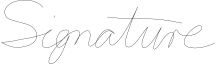
\includegraphics[width=6cm]{example_signature}\\

Date:	&\today\\
\end{tabular}
\vspace{6pt}

\makeatletter

% Can also use a copyright statement as below
%\hfill $\copyright$ Copyright \today{} \@author{}

\makeatother


\pagenumbering{roman}

\chapter*{Abstract}

This is the text of the abstract, providing a brief summary of the context, research problem, main contributions and conclusions of this work.


\chapter*{Dedication}

To my parents, for always loving and supporting me. 
To Mrtn Prd Grr


\chapter*{Acknowledgements}


I would like to thank Tristram Bogart for being an amazing advisor and for his guidance and support. Furthermore, a special thanks to John Goodrick for introducing me to the theory of computation and for his help and advice. In addition, a big thank you goes to the Polymath Jr. program, especially to Christopher O'Neill for introducing me to numerical semigroups, and to Johanna Franklin, for being cool mentors and for their support in guiding me into the world of research. I am also grateful to Alexander Getmanenko for his insightful seminars and book picks, to Adolfo Quiroz for his fun and engaging classes, as well as his advice, and to Monika Winklmeier, Ramiro de la Vega, Mauricio Velasco and Mauricio Junca for their exceptional teaching. Finally, I would like to extend my gratitude to my friends, who have made my undergraduate experience both fun and memorable. \par


{
\makeatletter
\vspace{1cm}
\raggedleft
\@author{}\\
\today{}\\
Bogotá, Colombia\\
\raggedright
\makeatother
}


\tableofcontents
%\listoffigures
%\listoftables

\pagenumbering{arabic}

% Add additional chapters as required
\chapter{Introduction}\label{chap:intro}


The Probabilistic Method is a powerful tool, with applications in Combinatorics, Graph Theory, Number Theory and Computer Science. It is a nonconstructive method that proves the existence of an object with a certain property, usually a graph, by showing that the probability that a randomly chosen object has that property is greater than zero. In this thesis, we will apply the probabilistic method to numerical semigroups. \par

A numerical semigroup is a subset of $\NN$ that is closed under addition (Definition \ref{def:smgps}). These objects are studied in the context of commutative algebra and algebraic geometry, and they have applications in integer programming, coding theory and cryptography \cite{assi2020numerical}. There are numerical invariants that are used to study numerical semigroups, such as the embedding dimension, the genus and the Frobenius number (Definitions \ref{def:smgps:embedding_dim}, \ref{def:smgps:genus} and \ref{def:smgps:frobeniusnum}). For example, the Frobenius number is defined as the maximum of the complement of the numerical semigroup over the integers. \par

The Erdös-Rényi (ER) model is a commonly used model of random graphs, where each edge is chosen with probability $p$, independently of the other edges (Definition \ref{def:probmet:ermodel}). In contrast to graphs, the study of random models of numerical semigroups requires the use of number theory tools due to their algebraic nature. This thesis investigates the average behavior of random numerical semigroup invariants using a probabilistic model similar to the ER model (Definition \ref{def:randnumsems:ermodel}).


Our central result is Theorem \ref{thm:main}, which is similar to Theorem \ref{thm:ermodel}, the main result of 
\begin{itemize}
    \item \fullcite{de2018random}.
\end{itemize}
Theorem \ref{thm:ermodel} describes the behavior of the expected embedding dimension, genus, and Frobenius number of a random numerical semigroup, depending on the parameters of the model. It gives an explicit bound of the expected value of these invariants. On the other hand, Theorem \ref{thm:main} describes the behavior of the invariants almost surely, that is, with probability that tends to one as the parameters of the model converge to certain values. Our proof is more elementary and provides asymptotically tighter bounds on the behaviour of these invariants. 

We used experiments to study the behavior of ER-type random numerical semigroups, which led to the proof of Theorem \ref{thm:main}. For our experiments, we used \verb|numsgps-sage| \cite[O'Neill]{oneill2018}\cite[Delgado]{delgado2015numericalsgps} and for visualizations we used \verb|IntPic| \cite[Delgado]{delgado2013intpic}. We also implemented our own publicly available repository \verb|randnumsgps| \cite{morales2023} for generating and visualizing random numerical semigroups in Python.\par

The structure of the thesis is as follows:

\begin{itemize}
    \item Chapter \ref{chap:probmet} discusses the Probabilistic Method, based on the work of Noga Alon and Joel H. Spencer.
    \item Chapter \ref{chap:numsems} focuses on numerical semigroups, providing definitions, examples, and results necessary for understanding their structure.
    \item Chapter \ref{chap:randnumsems} introduces three models of random numerical semigroups, including our newly proposed model. We also present recent results in the field, including Theorem \ref{thm:ermodel}. 
    \item Chapter \ref{chap:experiments} details the algorithms and experiments conducted.
    \item Chapter \ref{chap:results} presents the main results, including the proof of Theorem \ref{thm:main}, its implications and its relation with Theorem \ref{thm:ermodel}.
\end{itemize}

To sum up, we provide a detailed study of random numerical semigroups using probabilistic models, experimental data and software tools.\par


\chapter{The Probabilistic Method}\label{chap:probmet}

\section{Introduction}\label{sec:probmet:intro}

The probabilistic method is a powerful tool, with applications in Combinatorics, Graph Theory, Number Theory and Computer Science. It is a nonconstructive method that proves the existence of an object with a certain property, by showing that the probability that a randomly chosen object has that property is greater than zero. The method requires an appropiate sample space and is best illustrated by an example: \par

\begin{definition}\label{def:tournament}
A \textit{tournament} is a directed graph $T$ on $n$ vertices such that for every pair of vertices $i, j \in V(T)$, exactly one of the edges $(i, j)$ or $(j, i)$ is in $E(T)$. \cite{alon2016probabilistic} 
\end{definition}

The name of a tournament comes from the fact that it can be thought of as a sports tournament where each vertex represents a team and each team plays every other team exactly once. The edge $(i, j)$ represents a win for team $i$ over team $j$. A tournament $T$ has property $S_k$ if for every subset $K \subseteq V(T)$ of size $k$, there is a vertex $v \in V(T)$ such that $(v, s) \in E(T)$ for all $s \in K$ \cite{alon2016probabilistic}. That is, for every set of $k$ teams there is a team that beats all of them. For example, the tournament in Figure \ref{fig:tournament} has property $S_1$ since every team is beaten by another team. \par

A natural question to ask is: is there a tournament with property $S_k$ for every $k$? The answer is yes. We will prove this using the probabilistic method. First we define a probability space over the set of tournaments on $n$ vertices: \par 
A \textit{random} tournament on a set of $n$ vertices is a tournament $T$ such that for every pair of vertices $i, j \in V(T)$, the edge $(i, j)$ is in $E(T)$ with probability $\frac{1}{2}$ and the edge $(j, i)$ is in $E(T)$ with probability $\frac{1}{2}$, independently of all other edges. Thus, every tournament on $n$ vertices has the same probability, which means that this probability space is \textit{symmetric}. \par

\begin{figure}
    \centering
    \[\begin{tikzcd}
        & \bullet \\
        \\
        \bullet && \bullet
        \arrow[from=3-1, to=1-2]
        \arrow[from=1-2, to=3-3]
        \arrow[from=3-3, to=3-1]
    \end{tikzcd}\]
    \caption{A tournament on 3 vertices with property $S_1$.}
    \label{fig:tournament}
\end{figure}

The main idea is to show that there is a large $n$ as a function of $k$, such that the probability that a random tournament on $n$ vertices has property $S_k$ is greater than zero. This implies that there is at least one tournament with property $S_k$. \par


\begin{theorem}
    For every $k \in \N$, there is a tournament with property $S_k$. \cite{alon2016probabilistic}
\end{theorem}

\textbf{Proof. } Fix a subset $K \subseteq V(T)$ of size $k$. Consider the event $A_K$ that there is no vertex $v \in V(T)$ such that $(v, s) \in E(T)$ for all $s \in S$. For any vertex $v \in V(T) \setminus K$, the probability that $(v, s) \notin E(T)$ for all $s \in K$ is $2^{-k}$. Thus,
\[\Pr[A_K] = \left(1 - 2^{-k}\right)^{n - k}.\]
Now, if we consider all subsets $K \subseteq V(T)$ of size $k$, then the probability that $T$ does not have property $S_k$ is the probability that any of the events $A_K$ occurs. Since there are $\binom{n}{k}$ such subsets, by the union bound,
\[\Pr\left[\bigvee_{\substack{K \subseteq V(T) \\ |K| = k}} A_K\right] \leq \sum_{\substack{K \subseteq V(T) \\ |K| = k}}\Pr[A_K] = \binom{n}{k}\left(1 - 2^{-k}\right)^{n - k}.\]
We want to show that, for some $n$, this probability of this event is less than 1. Using Propositions \ref{ap:prop:upperbinom} and \ref{ap:prop:exp}, we have that
\begin{align}
    \Pr\left[\bigvee_{\substack{K \subseteq V(T) \\ |K| = k}} A_K\right] &\leq \binom{n}{k}\left(1 - 2^{-k}\right)^{n - k} \\
    &\leq \left(\frac{en}{k}\right)^k\left(e^{-2^{-k}}\right)^{n - k} = e^{k\log\left(\frac{n}{k}\right) - \frac{n - k}{2^k}}. \label{eq:tournament}
\end{align}
Then, \ref{eq:tournament} is less than one if 
\[k\log\left(\frac{n}{k}\right) - \frac{n - k}{2^k} = k\log n - k\log k + \frac{k}{2^k} - \frac{n}{2^k} < k\log n - \frac{n}{2^k} < 0,\]
which holds if and only if
\[\frac{n}{\log n} > k2^k.\]
Now, if $n = k^2 2^k\log 2$, then
\[\lim_{n \to \infty} \frac{n}{k2^k\log n} = \lim_{k \to \infty} \frac{k\log 2}{2\log k + k\log 2 + \log\log 2} = 1.\]
Hence, we conclude that there exists $n = (\log 2)k^2 2^k (1 + o(1))$, such that the probability that a random tournament on $n$ vertices does not have property $S_k$ is less than one. Therefore, the probability that there exists a tournament on $n$ vertices with property $S_k$ is greater than zero, which means that there exists at least one tournament with property $S_k$. \qed

We make two observations: 
\begin{enumerate}
    \item We used the \textit{union bound}. The union bound is a common technique in the probabilistic method. It states that for any events $A_1, ..., A_n$,
    \[\Pr[A_1 \cup ... \cup A_n] \leq \Pr[A_1] + ... + \Pr[A_n].\]
    We will extensively use this technique in this thesis. In a measure space, the union bound is the same property as \textit{subadditivity}. \par
    \item The proof is nonconstructive. It does not give us a way to find a tournament with property $S_k$. It only shows that there is at least one. This is a common feature of the probabilistic method. However, in this case, we have that for large enough $n$, the probability that a random tournament on $n$ vertices has property $S_k$ is close to one. This means that we can find a tournament with property $S_k$ by generating random tournaments until we find one with the desired property. If $n$ is large enough, this will not take too long. \par
\end{enumerate}
In this chapter, we will introduce some tools that are useful for applying the probabilistic method in discrete settings. We will also give some examples of the method in action. \par

\section{Linearity of Expectation}\label{sec:probmet:linearity}

Let $X$ be a discrete random variable, then the \textit{expected value} of $X$ is defined as 
\[E[X] = \sum_{x \in \text{Rg}(X)} x\Pr[X = x].\]
We show that the expected value is linear. \par
Let $X$ and $Y$ be discrete random variables. Then, the expected value of $X + Y$ is
\begin{align*}
    E[X + Y] &= \sum_{x \in \text{Rg}(X)} \sum_{y \in \text{Rg}(Y)} (x + y)\Pr[X = x \wedge Y = y] \\
    &= \sum_{x \in \text{Rg}(X)} \sum_{y \in \text{Rg}(Y)} x\Pr[X = x \wedge Y = y] + \sum_{x \in \text{Rg}(X)} \sum_{y \in \text{Rg}(Y)} y\Pr[X = x \wedge Y = y] \\
    &= \sum_{x \in \text{Rg}(X)} x\sum_{y \in \text{Rg}(Y)} \Pr[X = x \wedge Y = y] + \sum_{y \in \text{Rg}(Y)} y\sum_{x \in \text{Rg}(X)} \Pr[X = x \wedge Y = y] \\
    &= \sum_{x \in \text{Rg}(X)} x\Pr[X = x] + \sum_{y \in \text{Rg}(Y)} y\Pr[Y = y] \\
    &= E[X] + E[Y].
\end{align*}
Similarly, if $a \in \R$,
\begin{align*}
    E[aX] &= \sum_{x \in \text{Rg}(X)} ax\Pr[X = x] \\
    &= a\sum_{x \in \text{Rg}(X)} x\Pr[X = x] \\
    &= aE[X].
\end{align*}
This result is known as the \textit{linearity of expectation}. 
\begin{example}\label{ex:probmet:linearity}\cite{alon2016probabilistic}
    Let $\sigma$ be a random permutation of $\{1, \ldots, n\}$ chosen uniformly at random. Let $X_i$ be the indicator variable for the event that $\sigma(i) = i$. Then, $E[X_i] = \frac{1}{n}$ since there are $n$ possible values for $\sigma(i)$ and only one of them is $i$. Now, let $X = \sum_{i = 1}^n X_i$. Then, $X$ is the number of fixed points of $\sigma$. By the linearity of expectation,
    \[E[X] = E\left[\sum_{i = 1}^n X_i\right] = \sum_{i = 1}^n E[X_i] = \sum_{i = 1}^n \frac{1}{n} = 1.\tqed\]
\end{example}
Note that there is a point in the probability space $x \geq E[X]$ such that $\Pr[X = x] > 0$, and there is a point $x \leq E[X]$ such that $\Pr[X = x] > 0$. The following result by Szele (1943) is often considered as one of the first applications of the probabilistic method \cite{alon2016probabilistic}. \par
\begin{theorem}
    There is a tournament with $n$ players and at least $n!2^{-(n - 1)}$ Hamiltonian paths. \cite{alon2016probabilistic}
\end{theorem}
\textbf{Proof. } Let $X$ be the number of hamiltonian paths in a random tournament. Let $\sigma$ be a permutation, and let $X_\sigma$ be the indicator variable for the event that $\sigma$ is a hamiltonian path. That is, $\sigma$ is an ordering of the vertices such that $(\sigma(1), \sigma(2)), ..., (\sigma(n - 1), \sigma(n))$ are edges of the tournament. Then, $X = \sum_{\sigma} X_\sigma$. By the linearity of expectation,
\[E[X] = E\left[\sum_{\sigma} X_\sigma\right] = \sum_{\sigma} E[X_\sigma] = \sum_{\sigma} \frac{1}{2^{n - 1}} = n!2^{-(n - 1)}.\]
Therefore, there exists a tournament with at least $n!2^{-(n - 1)}$ hamiltonian paths. \qed

\section{Second Moment Method}\label{sec:probmet:secondmoment}

Just as we can use the linearity of expectation to prove results with the probabilistic method, we can also use the \textit{second moment method}, which relies on the \textit{variance} of a random variable. Let $X$ be a random variable with expected value $E[X]$. Then, the variance of $X$ is defined as
\[\text{Var}[X] = E[(X - E[X])^2].\]
By the linearity of expectation, 
\[E[(X - E[X])^2] = E[X] - 2E[XE[X]] + E[X]^2 = E[X^2] - E[X]^2.\]
The standard practice is to denote the expected value as $\mu$ and the variance as $\sigma^2$. The use of the following inequality is called the second moment method: \par

\begin{theorem}[Chebyschev's inequality]\label{thm:probmet:chebyschev}\cite{alon2016probabilistic}
    For $\lambda \geq 0$,
\end{theorem}
\[\Pr[|X - \mu| \geq \lambda \sigma] \leq \frac{1}{\lambda^2}.\]
\textbf{Proof. } 
\[\sigma^2 = \text{Var}[X] = E[(x - \mu)^2] \geq \lambda^2\sigma^2 \Pr[|X - \mu| \geq \lambda \sigma]. \qed\]

If $X = X_1 + ... + X_n$, then, by the linearity of expectation,
\[\text{Var}[X] = \sum_{i = 1}^{n}\text{Var}[X_i] + \sum_{i \neq j}\text{Cov}[X_i, X_j],\]
where 
\[\text{Cov}[X_i, X_j] = E[X_iX_j] - E[X_i]E[X_j].\] 
Furthermore, if, for each $i$, $X_i$ is an indicator variable of event $A_i$, that is, $X_i = 1$ if $A_i$ occurs and $X_i = 0$ otherwise, then
\[\text{Var}[X_i] = \Pr[A_i](1 - \Pr[A_i]) \leq E[X_i],\]
and we have that
\[\text{Var}[X] \leq E[X] + \sum_{i \neq j} \text{Cov}[X_i, X_j].\]

If $X$ only takes nonnegative integer values, we can bound $\Pr[X = 0]$ 

\section{Threshold Functions}\label{sec:probmet:threshold}

Let $n \in \N$ and $0 \leq p \leq 1$. The random graph $G(n, p)$ is a probability space over the set of graphs on $n$ labeled vertices determined by
\[\Pr[\{i, j\} \in G] = p\] 
with these events mutually independent \cite{alon2016probabilistic}. Given a graph theoretic property $A$, there is a probability that $G(n, p)$ satisfies $A$, which we write as $\Pr[G(n, p) \vDash A]$. 

\begin{definition}
    $r(n)$ is a threshold function for a graph theoretic property $A$ if 
    \begin{enumerate}
        \item When \(p(n) \in o(r(n)), \; \lim_{n \to \infty} \Pr[G(n, p(n)) \vDash A] = 0,\)
        \item When \(r(n) \in o(p(n)), \;  \lim_{n \to \infty} \Pr[G(n, p(n)) \vDash A] = 1,\) 
    \end{enumerate}
    or vice versa. \cite{alon2016probabilistic}
\end{definition}

We give an example of a threshold function which illustrates a common method for proving that a function is a threshold. \par

\subsection{Threshold function for having isolated vertices}

Let $G$ be a graph on $n$ labeled vertices. An isolated vertex of $G$ is a vertex which does not belong to any of the edges of $G$. Let $A$ be the property that $G$ contains an isolated vertex. We will prove that $\displaystyle{r(n) = \frac{\ln n}{n}}$ is a threshold for $A$. \par

For each vertex $i$ in $G$ define the variable 

\[X_i = 
\left\{
	\begin{array}{ll}
		1  & \mbox{if } i \text{ is an isolated vertex,} \\
		0 & \mbox{if } i \text{ is not an isolated vertex.}
	\end{array}
\right.
\]

Now, the probability that a vertex $i$ is isolated is $(1 - p)^{n - 1}$ since it is the probability that none of the other $n - 1$ vertices is connected to $i$. Let $X = \sum_{i = 1}^n X_i$, then the expected number of isolated vertices is
 \[E[X] = \sum_{i = 1}^{n} E[X_i] = \sum_{i = 1}^{n} \Pr[X_i] = n(1 - p)^{n - 1}.\]

Let $\displaystyle{p = k\frac{\ln n}{n}}$ for $k \in \R_{>0}$. Then
\begin{align*}
    \lim_{n \to \infty} E[X] &= \lim_{n \to \infty} n\left(1 - k\frac{\ln n}{n}\right)^{n - 1} \\
    &= ne^{-k\ln n} = n^{1 - k}.
\end{align*}

Therefore, $\lim_{n \to \infty} E[X] = 0$ if $k > 1$. Since \(E[X] \geq \Pr[X > 0],\) we conclude that \[\lim_{n \to \infty} \Pr[G(n, p) \vDash A] =  \lim_{n \to \infty} \Pr[X > 0] = 0.\] \par
Now, for $k < 1$, the fact that $\lim_{n \to \infty} E[X] = \infty$ is not enough to conclude that \(\lim_{n \to \infty} \Pr[G(n, p) \vDash A] = 1\). We have to use the second moment method. \par

\begin{theorem*}
    If $E[X] \to \infty$ and $\text{Var}[X] = o(E[X]^2)$, then $\lim_{n \to \infty} \Pr[X > 0] = 1$. \cite{alon2016probabilistic}
\end{theorem*}

\textbf{Proof. } We will prove that, in this case, $Var[X] = o(E[X]^2)$. First, 
\begin{align*}
    \sum_{i \neq j}E[X_iX_j] &= \sum_{i \neq j} \Pr[X_i = X_j = 1] \\
    &= n(n - 1)(1 - p)^{n -1}(1 - p)^{n - 2} \\ &= n(n - 1)(1 - p)^{2n - 3},
\end{align*}

for if $i$ is an isolated vertex, then there is no edge between $i$ and $j$ so we only have to account for the remaining $n - 2$ edges that contain $j$.  \par

Thus, since $\sum_{i = 1}^{n}E[X_i^2] =  \sum_{i = 1}^n E[X_i] = E[X]$ and $\lim_{n \to \infty} p = 0$,

\begin{align*}
    \lim_{n \to \infty} \frac{\text{Var}[X]}{E[X]^2} &= 
    \lim_{n \to \infty}\frac{E[X^2] - E[X]^2}{E[X]^2} = \lim_{n \to \infty} \frac{\sum_{i = 1}^n E[X_i^2] + \sum_{i \neq j}E[X_iX_j]}{E[X]^2} - 1 \\ &= 0 + \lim_{n \to \infty} \frac{ n(n - 1)(1 - p)^{2n - 3}}{n^2(1 - p)^{2n - 2}} - 1= \lim_{n \to \infty} \frac{1}{1 - p} - 1 = 0.\\
\end{align*} \par
We conclude that $\text{Var}[X] \in o(E[X]^2)$ and so, if $k < 1$, \[\lim_{n \to \infty} \Pr[G(n, p) \vDash A] = \lim_{n \to \infty} \Pr[X > 0] = 1.\] Therefore, $r(n) = \frac{\ln n}{n}$ is a threshold function for property $A$.


\chapter{Numerical Semigroups}\label{chap:probmet}

\section{Introduction}\label{sec:probmet:intro}

Some contextural overview of what we are going to discuss. Include the first example in the book. 

Section \ref{sec:litrev:theme1} discusses Theme 1. Section \ref{sec:litrev:theme2} discusses Theme 2....

A \textit{numerical semigroup} is a subset $S \subseteq \NN_{0}$ which is closed under addition, i.e. $a, b \in S$ implies $a + b \in S$. For instance, $\NN_0$, $\NN_0 \setminus \{0\}$, $2\NN_0$ are all numerical semigroups, but $\NN_0 \setminus \{2\}$ is not. Some literature requires that a semigroup has a finite complement in $\Z_{\geq 0}$ \cite{chapman2020beyond}, but we prefer the more general definition. 


\section{Invariants}\label{sec:probmet:theme1}


\subsection{Subtopic A}\label{sec:probmet:theme1:A}

\subsection{Subtopic B}\label{sec:probmet:theme1:B}

\subsection{Subtopic C}\label{sec:probmet:theme1:C}

\section{Wilf's Conjecture}\label{sec:probmet:theme2}

Etc. etc.


% All contribution chapters should follow a similar structure, with a
% mini-introduction and overview at the beginning and a conclusion at the
% end bookmarking a structured presentation of the contribution. This can be
% largely based on your publications.

\chapter{Random Numerical Semigroups}\label{chap:randnumsems}

We present three distinct models of random numerical semigroups. The first model employs a uniform distribution for its generators and is the most extensively studied. The second model is inspired by the Erdös-Rényi approach to random graphs. The third model is a new approach we introduce, characterized by a fixed Frobenius number.

\section{Box Model}\label{sec:randomsmpgs:intro}

Let $n, T \in \NN$. We consider the set of points
\[G(T) = \{A\in \NN^n : \mathrm{gcd}(A) = 1, \; |A|_\infty \leq T\}.\]
This is the set of possible sets of $n$ generators of numerical semigroups such that each generator is at most $T$. 
\begin{definition}\label{def:randnumsems:boxmodel}
    A Box model random numerical semigroup $\mathcal{S}(T)$ is a probability space over the set of semigroups $\mathcal{S} = \langle\mathcal{A}\rangle$ with $\mathcal{A} \in G(T)$, determined by
    \[\Pr[ \mathcal{A}] = \frac{1}{|G(T)|}.\]
\end{definition}
In other words, a point in $G(T)$ is chosen uniformly at random and the corresponding semigroup is returned. V. I. Arnold was the first to study this model \cite{arnold1999weak}. For any numerical semigroup, for $\mathcal{A} = \{a_1, \ldots, a_n\}$ such that $a_1 \leq \ldots \leq a_n$, Erdös and Graham \cite{erdos1972linear} proved that: 
\[F(\langle\mathcal{A} \rangle)  \leq 2 a_n\left[\frac{a_1}{n}\right]  - a_1.\]
On the other hand, Aliev and Gruber \cite{aliev2007optimal} proved an optimal lower bound for the Frobenius number, namely:
\[F(\langle\mathcal{A} \rangle)  > (n - 1)!^{\frac{1}{n - 1}}(a_1\cdots a_n)^{\frac{1}{n - 1}} - (a_1 + \cdots + a_n).\]
In \cite{arnold1999weak} and \cite{arnold2004arnold}, Arnold conjectured that the average behavior of the Frobenius number is, up to a constant, given by the lower bound, i.e.:
\[F(\langle\mathcal{A}\rangle) \sim (n - 1)!^{\frac{1}{n - 1}}(a_1\cdots a_n)^{\frac{1}{n - 1}}.\]
In 2009, Aliev, Henk and Hindrichs \cite{aliev2011expected} proved Arnold's conjecture, by showing the following theorem. 
% Expected Frobenius number results
\begin{theorem} Let $n \geq 3$. Then, for every constant $D$,
    \[\Pr\left[\frac{F(\langle\mathcal{A}\rangle)}{(a_1\cdots a_n)^{\frac{1}{n - 1}}}\geq D\right]  \in o(D^{-2\frac{n - 1}{n + 1}}).\]
\end{theorem}
The statement of this theorem does not depend on $T$, it only depends on $n$. The proof is based on a discrete inverse arithmetic-geometric mean inequality.

\section{ER-type model}

In order to use methods such as those that apply to the Erdös-Rényi model for random graphs, a similar model for random numerical semigroups was proposed in \cite{de2018random}. 

\begin{definition}\label{def:randnumsems:ermodel}
    For $p \in [0, 1]$ and $M \in \NN$, an ER-type random numerical semigroup $\mathcal{S}(M, p)$ is a probability space over the set of semigroups $\mathcal{S} = \langle\mathcal{A}\rangle$ with $\mathcal{A} \subseteq \{1,...,M\}$, determined by
    \[\Pr[n \in \mathcal{A}] = p,\]
    with these events mutually independent.
\end{definition}
Note that this definition does not require a numerical semigroup $\mathcal{S}$ to be co-finite. A semigroup $\mathcal{S}(M, p)$ is obtained by using the following procedure:
\begin{enumerate}
    \item Initialize an empty set $\mathcal{A}$.
    \item As $i$ goes from $1$ to $M$, add $i$ to $\mathcal{A}$ with probability $p$, independently of the other steps.
    \item Return the semigroup $\mathcal{S} = \langle\mathcal{A}\rangle$.
\end{enumerate}

The main result of \cite{de2018random} is the following theorem.  

\begin{theorem}\label{thm:ermodel} Let $\mathcal{S} \sim \mathcal{S}(M, p)$, where $p = p(M)$ is a monotone decreasing function of $M$. Then, 
    \begin{enumerate}[label=(\alph*)]
        \item If $p(M) \in o\left(\frac{1}{M}\right)$, then $\mathcal{S} = \{0\}$ almost always.
        \item If $\frac{1}{M} \in o(p(M))$ and $\lim_{M \to \infty} p(M)= 0$, then $\mathcal{S}$ is co-finite almost always and
         \[\lim_{M \to  \infty} \EE[e(\mathcal{S})] = \lim_{M \to \infty} \EE[g(\mathcal{S})] = \lim_{M \to \infty} \EE[F(\mathcal{S})] = \infty.\]
        \item If $\lim_{M \to \infty} p(M) > 0$, then
        \[\lim_{M \to \infty} \EE[e(\mathcal{S})] < \infty,  \quad \lim_{M \to \infty} \EE[g(\mathcal{S})] < \infty \quad  \text{ and } \quad \lim_{M \to \infty} \EE[F(\mathcal{S})]< \infty,\]
        and each limit is bounded by explicit rational functions in $p$.
    \end{enumerate}
\end{theorem}

Note that this proves that $\frac{1}{M}$ is a threshold function for co-finiteness, if we extend the definition of threshold functions of random graphs (Definition \ref{def:probmet:threshold}) to ER-type random numerical semigroups. The proof of this part of the theorem follows from standard arguments using the probabilistic method (Theorem \ref{thm:ermodel:co-finite}). \par
On the other hand, parts (b) and (c) follow from the construction of a shellable simplicial complex ( \cite[Definition 8]{de2018random}) whose facets are in bijection with irreducible numerical semigroups of a fixed Frobenius number $n$ (Definition \ref{def:smgps:irreducible}). It turns out that the faces of the $n-$th simplicial complex count the number of sets $\mathcal{A} \subset \{1, \ldots, n - 1\}$ satisfying $n \notin \langle\mathcal{A} \rangle$ (\cite[Proposition 23]{de2018random}). Thus, the expected value of the embedding dimension can be calculated from the entries of the $h$-vector (in the sense of algebraic combinatorics \cite{stanley2007combinatorics}) of this simplicial complex. \par

The authors also provide bounds for the expected value of the embedding dimension and the genus, when $p$ is constant.

\begin{theorem}\label{thm:ermodel:constantp}
    Let $\mathcal{S} \sim \mathcal{S}(M, p)$, where $p$ is a constant. Then, 
    \begin{align*}
        \frac{6 - 8p + 3p^2}{2 - 2p^2 + p^3} &\leq \lim_{M \to \infty} \EE[e(\mathcal{S})] \leq \frac{2 - p^2}{p}, \\
        \frac{6 - 14p + 11p^2 - 3p^3}{2p - 2p^3 + p^4} &\leq \lim_{M \to \infty} \EE[g(\mathcal{S})] \leq \frac{(1 - p)(2 - p^2)}{p^2}, \text{ and}\\
        \frac{6 - 14p + 11p^2 - 3p^3}{2p - 2p^3 + p^4} &\leq \lim_{M \to \infty} \EE[f(\mathcal{S})] \leq \frac{2(1 - p)(2 - p^2)}{p^2}.
    \end{align*}
\end{theorem}
As $p$ tends to 0, this says that the limit of the expected value of the embedding dimension is between a function that tends to a constant and a function that is asymptotically linear in $\frac{1}{p}$. Also, the expected values of the genus and the Frobenius number are between a function that is asymptotically linear in $\frac{1}{p}$ and a function that is asymptotically quadratic in $\frac{1}{p}$. It is useful to think of these functions in terms of $\frac{1}{p}$, since it is the expected value of the gap between randomly selected elements of $\mathcal{A}$ in the ER-type model. \par 

We now prove part (a) of Theorem \ref{thm:ermodel}.

\begin{theorem}[Theorem 5 \cite{de2018random}]\label{thm:ermodel:co-finite}
     $\frac{1}{M}$ is a threshold function for co-finiteness.
\end{theorem}

\textbf{Proof. } We prove the two parts of the theorem separately. 
\subsubsection*{Part 1}
Suppose that $p \in o\left(\frac{1}{M}\right)$. As in Inequality \ref{eq:probmet:secondmoment:1}, 
\[\Pr[|\mathcal{A}| > 0] \leq \EE[|\mathcal{A}|] = Mp.\]
Since $Mp \to 0$ as $M \to \infty$, we have that $\Pr[|\mathcal{A}| > 0] \to 0$ as $M \to \infty$. Thus, $\mathcal{S} = \{0\}$ almost always. \par

\subsubsection*{Part 2}
Suppose that $\frac{1}{M} \in o(p)$ and $\lim_{M \to \infty} p = 0$. We prove that $\mathcal{S}$ is co-finite almost always, by showing that $\mathcal{A}$ almost always contains a co-prime pair of elements. \par
For each pair of distinct co-prime integers $i, j \in \{1,\ldots, m\}$, let $A_{i, j}$ be the event that $i, j \in \mathcal{A}$. Let $1_{i, j}$ be the indicator variable of event $A_{i, j}$ and let 
\[X = \sum_{\substack{i < j \\ \mathrm{gcd}(i, j) = 1}} 1_{i, j}.\]
We show that $X > 0$ almost always using the second moment method. First we calculate $\EE[X]$. It is a well-established result in number theory \cite[Theorem 332]{hardy1979introduction} that the limiting probability of two integers being co-prime is $\frac{6}{\pi^2}$. That is,
\[\lim_{M \to \infty} \frac{|\{(a, b) \in \{1, \ldots, M\}^2: \mathrm{gcd}(a, b) = 1\}|}{M^2} = \frac{1}{\zeta(2)} =\frac{6}{\pi^2}.\]
Therefore, $E[X] \sim \frac{3}{\pi^2}M^2p^2$. Now, $\{i, j\} \sim \{i', j'\}$ (see (\ref{eq:probmet:delta})) if $i = i'$ and $j \neq j'$. Thus, by varying over triples $i, j, j'$, we obtain
\[\Delta = \sum_{\{i, j\} \sim \{i', j'\}}\Pr[A_{i, j}\land A_{i', j'}] \leq M^3p^3.\]
Therefore, $\Delta \in o(\EE[X]^2)$, since $\frac{1}{M} \in o(p)$. Thus, by the second moment method (Corollary \ref{cor:probmet:secondmoment:3}), $X > 0$ almost always. This means that $\mathcal{A}$ almost always contains a co-prime pair of elements and so $\mathcal{S}$ is co-finite. \qed \par

In chapter \ref{chap:results}, we prove part (b) of Theorem \ref{thm:ermodel} using standard probabilistic methods. We also prove a result related to part (c) (Lemma \ref{lem:upperbound}) .

\section{Downward model}\label{sec:contrib1:theme2}

We propose a new model for random numerical semigroups that fixes the Frobenius number, which could be helpful in the study of Wilf's conjecture. We have not yet proved any results about this model, but we present some experiments in Chapter \ref{chap:experiments}.

\begin{definition} Fix $f \in \NN$, then the downward random numerical semigroup $\mathcal{S}_\downarrow(f, p)$ is defined by the following procedure: 
\begin{enumerate}
    \item Initialize a set $\mathcal{A} = \{f + 1, \ldots, 2f, 2f + 1\}$.
    \item As $i$ goes down from $f - 2$ to $1$. If $F(\langle A \cup \{i\} \rangle) = f$, add $i$ to $\mathcal{A}$ with probability $p$. Otherwise, proceed to the next step.
    \item Return the semigroup $\mathcal{S} = \langle\mathcal{A}\rangle$.
\end{enumerate}
Step 1 initializes the minimal numerical semigroup (with respect to inclusion) such that $f(\mathcal{S}) = f$. Step 2 randomly adds elements to $\mathcal{A}$ in decreasing order, such that $F(\langle A \cup \{i\} \rangle) = f$. Note that in this case, the probability of adding an element to $\mathcal{A}$ is not independent of the other steps. 
    
\end{definition}



% All contribution chapters should follow a similar structure, with a
% mini-introduction and overview at the beginning and a conclusion at the
% end bookmarking a structured presentation of the contribution. This can be
% largely based on your publications.
\lstset{
	tabsize=4,
	rulecolor=,
	language=Python,
	basicstyle=\tiny,
	upquote=true,
	aboveskip={1.5\baselineskip},
	columns=fixed,
	showstringspaces=false,
	extendedchars=true,
	breaklines=true,
	prebreak = \raisebox{0ex}[0ex][0ex]{\ensuremath{\hookleftarrow}},
	frame=single,
	showtabs=false,
	showspaces=false,
	showstringspaces=false,
	identifierstyle=\ttfamily,
	keywordstyle=\color[rgb]{0,0,1},
	commentstyle=\color[rgb]{0.133,0.545,0.133},
	stringstyle=\color[rgb]{0.627,0.126,0.941},
	numbers=left, numberstyle=\tiny, stepnumber=1,
	numbersep=5pt
}


\chapter{Experiments}\label{chap:experiments}

\section{ER-type model experiments}

We used the following algorithm for ER-type random numerical semigroup generation (see Definition \ref{def:probmet:ermodel}). The \verb|NumericalSemigroup| class is part of the \verb|numsgps-sage| package \cite{oneill2018}. 

\begin{lstlisting}[language=Python]
    # Generates random sample using Erdös-Rényi model 
    def generate_sample(M, p, sample_size):
        semigroups = []
        for j in range(sample_size):
            generators = []
            for i in range(M):
                if random.random() < p:
                    generators.append(i)
            if gcd(generators) != 1:
                continue
            semigroups.append(NumericalSemigroup(generators))
        return semigroups
\end{lstlisting}
We generated random numerical semigroups for several values of $1/p$ in the range $[4, 1000]$. For each $1/p$, the sample size was 1000 and we calculated the average embedding dimension (Table \ref{tab:embedding}) and the average Frobenius number (Table \ref{tab:frobenius}). As shown in \cite{de2018random}, the bounds found in Theorem \ref{thm:ermodel:constantp} are not tight. We plot the average embedding dimension and the average Frobenius number for each $1/p$ in Figures \ref{fig:embedding} and \ref{fig:frobenius}. We also plot the histograms of the embedding dimension and the Frobenius number for $1/p = 4, 220, 1000$ in Figures \ref{fig:embedding_hist4}, \ref{fig:embedding_hist220}, \ref{fig:embedding_hist1000}, \ref{fig:frobenius_hist4}, \ref{fig:frobenius_hist220}, \ref{fig:frobenius_hist1000}. \par
Write a paragraph saying why we are making this proofs. 

\begin{table}
\centering
\begin{tabular}{|c|c|c|c|}
    \hline
    $1/p$ & Lower Bound & $\overline{e(\mathcal{S})}$  & Upper bound \\
    \hline
    4.00 & 2.21 & 2.79 & 7.75 \\
    75.14 & 2.95 & 9.05 & 150.27 \\
    146.29 & 2.97 & 10.67 & 292.56 \\
    217.43 & 2.98 & 12.28 & 434.85 \\
    288.57 & 2.99 & 12.94 & 577.14 \\
    359.71 & 2.99 & 13.65 & 719.43 \\
    430.86 & 2.99 & 14.14 & 861.71 \\
    502.00 & 2.99 & 14.73 & 1,004.00 \\
    573.14 & 2.99 & 15.29 & 1,146.28 \\
    644.29 & 2.99 & 16.17 & 1,288.57 \\
    715.43 & 2.99 & 16.07 & 1,430.86 \\
    786.57 & 2.99 & 16.34 & 1,573.14 \\
    857.71 & 3.00 & 16.61 & 1,715.43 \\
    928.86 & 3.00 & 17.39 & 1,857.71 \\
    1,000.00 & 3.00 & 17.22 & 2,000.00 \\
    \hline
\end{tabular}
\caption{Average embedding dimension of random numerical semigroups generated using the ER-type model.}
\label{tab:embedding}
\end{table}

Frobenius number:
\begin{table}
\centering
\begin{tabular}{|c|c|c|c|}
    \hline
    $1/p$ & Lower Bound & $\overline{F(\mathcal{S})}$ & Upper bound \\
    \hline
    4.00 & 7.26 & 13.96 & 46.50 \\
    75.14 & 218.56 & 1,088.82 & 22,283.25 \\
    146.29 & 431.93 & 2,483.26 & 85,010.91 \\
    217.43 & 645.33 & 4,174.94 & 188,229.03 \\
    288.57 & 858.75 & 5,859.29 & 331,937.60 \\
    359.71 & 1,072.17 & 7,794.18 & 516,136.62 \\
    430.86 & 1,285.59 & 9,594.56 & 740,826.09 \\
    502.00 & 1,499.02 & 11,533.38 & 1,006,006.00 \\
    573.14 & 1,712.45 & 13,765.73 & 1,311,676.37 \\
    644.29 & 1,925.87 & 16,239.19 & 1,657,837.19 \\
    715.43 & 2,139.30 & 17,769.34 & 2,044,488.45 \\
    786.57 & 2,352.73 & 19,806.19 & 2,471,630.17 \\
    857.71 & 2,566.15 & 22,157.78 & 2,939,262.33 \\
    928.86 & 2,779.58 & 25,079.10 & 3,447,384.94 \\
    1,000.00 & 2,993.01 & 26,637.46 & 3,995,998.00 \\
    \hline
\end{tabular}
\caption{Average Frobenius number of random numerical semigroups generated using the ER-type model.}
\label{tab:frobenius}
\end{table}

\begin{figure}
    \begin{center}
        %% Creator: Matplotlib, PGF backend
%%
%% To include the figure in your LaTeX document, write
%%   \input{<filename>.pgf}
%%
%% Make sure the required packages are loaded in your preamble
%%   \usepackage{pgf}
%%
%% Also ensure that all the required font packages are loaded; for instance,
%% the lmodern package is sometimes necessary when using math font.
%%   \usepackage{lmodern}
%%
%% Figures using additional raster images can only be included by \input if
%% they are in the same directory as the main LaTeX file. For loading figures
%% from other directories you can use the `import` package
%%   \usepackage{import}
%%
%% and then include the figures with
%%   \import{<path to file>}{<filename>.pgf}
%%
%% Matplotlib used the following preamble
%%
\begingroup%
\makeatletter%
\begin{pgfpicture}%
\pgfpathrectangle{\pgfpointorigin}{\pgfqpoint{6.000000in}{4.000000in}}%
\pgfusepath{use as bounding box, clip}%
\begin{pgfscope}%
\pgfsetbuttcap%
\pgfsetmiterjoin%
\pgfsetlinewidth{0.000000pt}%
\definecolor{currentstroke}{rgb}{1.000000,1.000000,1.000000}%
\pgfsetstrokecolor{currentstroke}%
\pgfsetstrokeopacity{0.000000}%
\pgfsetdash{}{0pt}%
\pgfpathmoveto{\pgfqpoint{0.000000in}{0.000000in}}%
\pgfpathlineto{\pgfqpoint{6.000000in}{0.000000in}}%
\pgfpathlineto{\pgfqpoint{6.000000in}{4.000000in}}%
\pgfpathlineto{\pgfqpoint{0.000000in}{4.000000in}}%
\pgfpathlineto{\pgfqpoint{0.000000in}{0.000000in}}%
\pgfpathclose%
\pgfusepath{}%
\end{pgfscope}%
\begin{pgfscope}%
\pgfsetbuttcap%
\pgfsetmiterjoin%
\definecolor{currentfill}{rgb}{1.000000,1.000000,1.000000}%
\pgfsetfillcolor{currentfill}%
\pgfsetlinewidth{0.000000pt}%
\definecolor{currentstroke}{rgb}{0.000000,0.000000,0.000000}%
\pgfsetstrokecolor{currentstroke}%
\pgfsetstrokeopacity{0.000000}%
\pgfsetdash{}{0pt}%
\pgfpathmoveto{\pgfqpoint{0.773458in}{0.565123in}}%
\pgfpathlineto{\pgfqpoint{5.850000in}{0.565123in}}%
\pgfpathlineto{\pgfqpoint{5.850000in}{3.650926in}}%
\pgfpathlineto{\pgfqpoint{0.773458in}{3.650926in}}%
\pgfpathlineto{\pgfqpoint{0.773458in}{0.565123in}}%
\pgfpathclose%
\pgfusepath{fill}%
\end{pgfscope}%
\begin{pgfscope}%
\pgfsetbuttcap%
\pgfsetroundjoin%
\definecolor{currentfill}{rgb}{0.000000,0.000000,0.000000}%
\pgfsetfillcolor{currentfill}%
\pgfsetlinewidth{0.803000pt}%
\definecolor{currentstroke}{rgb}{0.000000,0.000000,0.000000}%
\pgfsetstrokecolor{currentstroke}%
\pgfsetdash{}{0pt}%
\pgfsys@defobject{currentmarker}{\pgfqpoint{0.000000in}{-0.048611in}}{\pgfqpoint{0.000000in}{0.000000in}}{%
\pgfpathmoveto{\pgfqpoint{0.000000in}{0.000000in}}%
\pgfpathlineto{\pgfqpoint{0.000000in}{-0.048611in}}%
\pgfusepath{stroke,fill}%
}%
\begin{pgfscope}%
\pgfsys@transformshift{0.985675in}{0.565123in}%
\pgfsys@useobject{currentmarker}{}%
\end{pgfscope}%
\end{pgfscope}%
\begin{pgfscope}%
\definecolor{textcolor}{rgb}{0.000000,0.000000,0.000000}%
\pgfsetstrokecolor{textcolor}%
\pgfsetfillcolor{textcolor}%
\pgftext[x=0.985675in,y=0.467901in,,top]{\color{textcolor}\rmfamily\fontsize{10.000000}{12.000000}\selectfont \(\displaystyle {0}\)}%
\end{pgfscope}%
\begin{pgfscope}%
\pgfsetbuttcap%
\pgfsetroundjoin%
\definecolor{currentfill}{rgb}{0.000000,0.000000,0.000000}%
\pgfsetfillcolor{currentfill}%
\pgfsetlinewidth{0.803000pt}%
\definecolor{currentstroke}{rgb}{0.000000,0.000000,0.000000}%
\pgfsetstrokecolor{currentstroke}%
\pgfsetdash{}{0pt}%
\pgfsys@defobject{currentmarker}{\pgfqpoint{0.000000in}{-0.048611in}}{\pgfqpoint{0.000000in}{0.000000in}}{%
\pgfpathmoveto{\pgfqpoint{0.000000in}{0.000000in}}%
\pgfpathlineto{\pgfqpoint{0.000000in}{-0.048611in}}%
\pgfusepath{stroke,fill}%
}%
\begin{pgfscope}%
\pgfsys@transformshift{1.912390in}{0.565123in}%
\pgfsys@useobject{currentmarker}{}%
\end{pgfscope}%
\end{pgfscope}%
\begin{pgfscope}%
\definecolor{textcolor}{rgb}{0.000000,0.000000,0.000000}%
\pgfsetstrokecolor{textcolor}%
\pgfsetfillcolor{textcolor}%
\pgftext[x=1.912390in,y=0.467901in,,top]{\color{textcolor}\rmfamily\fontsize{10.000000}{12.000000}\selectfont \(\displaystyle {200}\)}%
\end{pgfscope}%
\begin{pgfscope}%
\pgfsetbuttcap%
\pgfsetroundjoin%
\definecolor{currentfill}{rgb}{0.000000,0.000000,0.000000}%
\pgfsetfillcolor{currentfill}%
\pgfsetlinewidth{0.803000pt}%
\definecolor{currentstroke}{rgb}{0.000000,0.000000,0.000000}%
\pgfsetstrokecolor{currentstroke}%
\pgfsetdash{}{0pt}%
\pgfsys@defobject{currentmarker}{\pgfqpoint{0.000000in}{-0.048611in}}{\pgfqpoint{0.000000in}{0.000000in}}{%
\pgfpathmoveto{\pgfqpoint{0.000000in}{0.000000in}}%
\pgfpathlineto{\pgfqpoint{0.000000in}{-0.048611in}}%
\pgfusepath{stroke,fill}%
}%
\begin{pgfscope}%
\pgfsys@transformshift{2.839104in}{0.565123in}%
\pgfsys@useobject{currentmarker}{}%
\end{pgfscope}%
\end{pgfscope}%
\begin{pgfscope}%
\definecolor{textcolor}{rgb}{0.000000,0.000000,0.000000}%
\pgfsetstrokecolor{textcolor}%
\pgfsetfillcolor{textcolor}%
\pgftext[x=2.839104in,y=0.467901in,,top]{\color{textcolor}\rmfamily\fontsize{10.000000}{12.000000}\selectfont \(\displaystyle {400}\)}%
\end{pgfscope}%
\begin{pgfscope}%
\pgfsetbuttcap%
\pgfsetroundjoin%
\definecolor{currentfill}{rgb}{0.000000,0.000000,0.000000}%
\pgfsetfillcolor{currentfill}%
\pgfsetlinewidth{0.803000pt}%
\definecolor{currentstroke}{rgb}{0.000000,0.000000,0.000000}%
\pgfsetstrokecolor{currentstroke}%
\pgfsetdash{}{0pt}%
\pgfsys@defobject{currentmarker}{\pgfqpoint{0.000000in}{-0.048611in}}{\pgfqpoint{0.000000in}{0.000000in}}{%
\pgfpathmoveto{\pgfqpoint{0.000000in}{0.000000in}}%
\pgfpathlineto{\pgfqpoint{0.000000in}{-0.048611in}}%
\pgfusepath{stroke,fill}%
}%
\begin{pgfscope}%
\pgfsys@transformshift{3.765819in}{0.565123in}%
\pgfsys@useobject{currentmarker}{}%
\end{pgfscope}%
\end{pgfscope}%
\begin{pgfscope}%
\definecolor{textcolor}{rgb}{0.000000,0.000000,0.000000}%
\pgfsetstrokecolor{textcolor}%
\pgfsetfillcolor{textcolor}%
\pgftext[x=3.765819in,y=0.467901in,,top]{\color{textcolor}\rmfamily\fontsize{10.000000}{12.000000}\selectfont \(\displaystyle {600}\)}%
\end{pgfscope}%
\begin{pgfscope}%
\pgfsetbuttcap%
\pgfsetroundjoin%
\definecolor{currentfill}{rgb}{0.000000,0.000000,0.000000}%
\pgfsetfillcolor{currentfill}%
\pgfsetlinewidth{0.803000pt}%
\definecolor{currentstroke}{rgb}{0.000000,0.000000,0.000000}%
\pgfsetstrokecolor{currentstroke}%
\pgfsetdash{}{0pt}%
\pgfsys@defobject{currentmarker}{\pgfqpoint{0.000000in}{-0.048611in}}{\pgfqpoint{0.000000in}{0.000000in}}{%
\pgfpathmoveto{\pgfqpoint{0.000000in}{0.000000in}}%
\pgfpathlineto{\pgfqpoint{0.000000in}{-0.048611in}}%
\pgfusepath{stroke,fill}%
}%
\begin{pgfscope}%
\pgfsys@transformshift{4.692534in}{0.565123in}%
\pgfsys@useobject{currentmarker}{}%
\end{pgfscope}%
\end{pgfscope}%
\begin{pgfscope}%
\definecolor{textcolor}{rgb}{0.000000,0.000000,0.000000}%
\pgfsetstrokecolor{textcolor}%
\pgfsetfillcolor{textcolor}%
\pgftext[x=4.692534in,y=0.467901in,,top]{\color{textcolor}\rmfamily\fontsize{10.000000}{12.000000}\selectfont \(\displaystyle {800}\)}%
\end{pgfscope}%
\begin{pgfscope}%
\pgfsetbuttcap%
\pgfsetroundjoin%
\definecolor{currentfill}{rgb}{0.000000,0.000000,0.000000}%
\pgfsetfillcolor{currentfill}%
\pgfsetlinewidth{0.803000pt}%
\definecolor{currentstroke}{rgb}{0.000000,0.000000,0.000000}%
\pgfsetstrokecolor{currentstroke}%
\pgfsetdash{}{0pt}%
\pgfsys@defobject{currentmarker}{\pgfqpoint{0.000000in}{-0.048611in}}{\pgfqpoint{0.000000in}{0.000000in}}{%
\pgfpathmoveto{\pgfqpoint{0.000000in}{0.000000in}}%
\pgfpathlineto{\pgfqpoint{0.000000in}{-0.048611in}}%
\pgfusepath{stroke,fill}%
}%
\begin{pgfscope}%
\pgfsys@transformshift{5.619248in}{0.565123in}%
\pgfsys@useobject{currentmarker}{}%
\end{pgfscope}%
\end{pgfscope}%
\begin{pgfscope}%
\definecolor{textcolor}{rgb}{0.000000,0.000000,0.000000}%
\pgfsetstrokecolor{textcolor}%
\pgfsetfillcolor{textcolor}%
\pgftext[x=5.619248in,y=0.467901in,,top]{\color{textcolor}\rmfamily\fontsize{10.000000}{12.000000}\selectfont \(\displaystyle {1000}\)}%
\end{pgfscope}%
\begin{pgfscope}%
\definecolor{textcolor}{rgb}{0.000000,0.000000,0.000000}%
\pgfsetstrokecolor{textcolor}%
\pgfsetfillcolor{textcolor}%
\pgftext[x=3.311729in,y=0.288889in,,top]{\color{textcolor}\rmfamily\fontsize{10.000000}{12.000000}\selectfont \(\displaystyle 1/p\)}%
\end{pgfscope}%
\begin{pgfscope}%
\pgfsetbuttcap%
\pgfsetroundjoin%
\definecolor{currentfill}{rgb}{0.000000,0.000000,0.000000}%
\pgfsetfillcolor{currentfill}%
\pgfsetlinewidth{0.803000pt}%
\definecolor{currentstroke}{rgb}{0.000000,0.000000,0.000000}%
\pgfsetstrokecolor{currentstroke}%
\pgfsetdash{}{0pt}%
\pgfsys@defobject{currentmarker}{\pgfqpoint{-0.048611in}{0.000000in}}{\pgfqpoint{-0.000000in}{0.000000in}}{%
\pgfpathmoveto{\pgfqpoint{-0.000000in}{0.000000in}}%
\pgfpathlineto{\pgfqpoint{-0.048611in}{0.000000in}}%
\pgfusepath{stroke,fill}%
}%
\begin{pgfscope}%
\pgfsys@transformshift{0.773458in}{0.703969in}%
\pgfsys@useobject{currentmarker}{}%
\end{pgfscope}%
\end{pgfscope}%
\begin{pgfscope}%
\definecolor{textcolor}{rgb}{0.000000,0.000000,0.000000}%
\pgfsetstrokecolor{textcolor}%
\pgfsetfillcolor{textcolor}%
\pgftext[x=0.606791in, y=0.655744in, left, base]{\color{textcolor}\rmfamily\fontsize{10.000000}{12.000000}\selectfont \(\displaystyle {0}\)}%
\end{pgfscope}%
\begin{pgfscope}%
\pgfsetbuttcap%
\pgfsetroundjoin%
\definecolor{currentfill}{rgb}{0.000000,0.000000,0.000000}%
\pgfsetfillcolor{currentfill}%
\pgfsetlinewidth{0.803000pt}%
\definecolor{currentstroke}{rgb}{0.000000,0.000000,0.000000}%
\pgfsetstrokecolor{currentstroke}%
\pgfsetdash{}{0pt}%
\pgfsys@defobject{currentmarker}{\pgfqpoint{-0.048611in}{0.000000in}}{\pgfqpoint{-0.000000in}{0.000000in}}{%
\pgfpathmoveto{\pgfqpoint{-0.000000in}{0.000000in}}%
\pgfpathlineto{\pgfqpoint{-0.048611in}{0.000000in}}%
\pgfusepath{stroke,fill}%
}%
\begin{pgfscope}%
\pgfsys@transformshift{0.773458in}{1.211857in}%
\pgfsys@useobject{currentmarker}{}%
\end{pgfscope}%
\end{pgfscope}%
\begin{pgfscope}%
\definecolor{textcolor}{rgb}{0.000000,0.000000,0.000000}%
\pgfsetstrokecolor{textcolor}%
\pgfsetfillcolor{textcolor}%
\pgftext[x=0.398457in, y=1.163632in, left, base]{\color{textcolor}\rmfamily\fontsize{10.000000}{12.000000}\selectfont \(\displaystyle {5000}\)}%
\end{pgfscope}%
\begin{pgfscope}%
\pgfsetbuttcap%
\pgfsetroundjoin%
\definecolor{currentfill}{rgb}{0.000000,0.000000,0.000000}%
\pgfsetfillcolor{currentfill}%
\pgfsetlinewidth{0.803000pt}%
\definecolor{currentstroke}{rgb}{0.000000,0.000000,0.000000}%
\pgfsetstrokecolor{currentstroke}%
\pgfsetdash{}{0pt}%
\pgfsys@defobject{currentmarker}{\pgfqpoint{-0.048611in}{0.000000in}}{\pgfqpoint{-0.000000in}{0.000000in}}{%
\pgfpathmoveto{\pgfqpoint{-0.000000in}{0.000000in}}%
\pgfpathlineto{\pgfqpoint{-0.048611in}{0.000000in}}%
\pgfusepath{stroke,fill}%
}%
\begin{pgfscope}%
\pgfsys@transformshift{0.773458in}{1.719745in}%
\pgfsys@useobject{currentmarker}{}%
\end{pgfscope}%
\end{pgfscope}%
\begin{pgfscope}%
\definecolor{textcolor}{rgb}{0.000000,0.000000,0.000000}%
\pgfsetstrokecolor{textcolor}%
\pgfsetfillcolor{textcolor}%
\pgftext[x=0.329012in, y=1.671520in, left, base]{\color{textcolor}\rmfamily\fontsize{10.000000}{12.000000}\selectfont \(\displaystyle {10000}\)}%
\end{pgfscope}%
\begin{pgfscope}%
\pgfsetbuttcap%
\pgfsetroundjoin%
\definecolor{currentfill}{rgb}{0.000000,0.000000,0.000000}%
\pgfsetfillcolor{currentfill}%
\pgfsetlinewidth{0.803000pt}%
\definecolor{currentstroke}{rgb}{0.000000,0.000000,0.000000}%
\pgfsetstrokecolor{currentstroke}%
\pgfsetdash{}{0pt}%
\pgfsys@defobject{currentmarker}{\pgfqpoint{-0.048611in}{0.000000in}}{\pgfqpoint{-0.000000in}{0.000000in}}{%
\pgfpathmoveto{\pgfqpoint{-0.000000in}{0.000000in}}%
\pgfpathlineto{\pgfqpoint{-0.048611in}{0.000000in}}%
\pgfusepath{stroke,fill}%
}%
\begin{pgfscope}%
\pgfsys@transformshift{0.773458in}{2.227633in}%
\pgfsys@useobject{currentmarker}{}%
\end{pgfscope}%
\end{pgfscope}%
\begin{pgfscope}%
\definecolor{textcolor}{rgb}{0.000000,0.000000,0.000000}%
\pgfsetstrokecolor{textcolor}%
\pgfsetfillcolor{textcolor}%
\pgftext[x=0.329012in, y=2.179408in, left, base]{\color{textcolor}\rmfamily\fontsize{10.000000}{12.000000}\selectfont \(\displaystyle {15000}\)}%
\end{pgfscope}%
\begin{pgfscope}%
\pgfsetbuttcap%
\pgfsetroundjoin%
\definecolor{currentfill}{rgb}{0.000000,0.000000,0.000000}%
\pgfsetfillcolor{currentfill}%
\pgfsetlinewidth{0.803000pt}%
\definecolor{currentstroke}{rgb}{0.000000,0.000000,0.000000}%
\pgfsetstrokecolor{currentstroke}%
\pgfsetdash{}{0pt}%
\pgfsys@defobject{currentmarker}{\pgfqpoint{-0.048611in}{0.000000in}}{\pgfqpoint{-0.000000in}{0.000000in}}{%
\pgfpathmoveto{\pgfqpoint{-0.000000in}{0.000000in}}%
\pgfpathlineto{\pgfqpoint{-0.048611in}{0.000000in}}%
\pgfusepath{stroke,fill}%
}%
\begin{pgfscope}%
\pgfsys@transformshift{0.773458in}{2.735521in}%
\pgfsys@useobject{currentmarker}{}%
\end{pgfscope}%
\end{pgfscope}%
\begin{pgfscope}%
\definecolor{textcolor}{rgb}{0.000000,0.000000,0.000000}%
\pgfsetstrokecolor{textcolor}%
\pgfsetfillcolor{textcolor}%
\pgftext[x=0.329012in, y=2.687296in, left, base]{\color{textcolor}\rmfamily\fontsize{10.000000}{12.000000}\selectfont \(\displaystyle {20000}\)}%
\end{pgfscope}%
\begin{pgfscope}%
\pgfsetbuttcap%
\pgfsetroundjoin%
\definecolor{currentfill}{rgb}{0.000000,0.000000,0.000000}%
\pgfsetfillcolor{currentfill}%
\pgfsetlinewidth{0.803000pt}%
\definecolor{currentstroke}{rgb}{0.000000,0.000000,0.000000}%
\pgfsetstrokecolor{currentstroke}%
\pgfsetdash{}{0pt}%
\pgfsys@defobject{currentmarker}{\pgfqpoint{-0.048611in}{0.000000in}}{\pgfqpoint{-0.000000in}{0.000000in}}{%
\pgfpathmoveto{\pgfqpoint{-0.000000in}{0.000000in}}%
\pgfpathlineto{\pgfqpoint{-0.048611in}{0.000000in}}%
\pgfusepath{stroke,fill}%
}%
\begin{pgfscope}%
\pgfsys@transformshift{0.773458in}{3.243410in}%
\pgfsys@useobject{currentmarker}{}%
\end{pgfscope}%
\end{pgfscope}%
\begin{pgfscope}%
\definecolor{textcolor}{rgb}{0.000000,0.000000,0.000000}%
\pgfsetstrokecolor{textcolor}%
\pgfsetfillcolor{textcolor}%
\pgftext[x=0.329012in, y=3.195184in, left, base]{\color{textcolor}\rmfamily\fontsize{10.000000}{12.000000}\selectfont \(\displaystyle {25000}\)}%
\end{pgfscope}%
\begin{pgfscope}%
\definecolor{textcolor}{rgb}{0.000000,0.000000,0.000000}%
\pgfsetstrokecolor{textcolor}%
\pgfsetfillcolor{textcolor}%
\pgftext[x=0.273457in,y=2.108025in,,bottom,rotate=90.000000]{\color{textcolor}\rmfamily\fontsize{10.000000}{12.000000}\selectfont Experiments}%
\end{pgfscope}%
\begin{pgfscope}%
\pgfpathrectangle{\pgfqpoint{0.773458in}{0.565123in}}{\pgfqpoint{5.076542in}{3.085803in}}%
\pgfusepath{clip}%
\pgfsetrectcap%
\pgfsetroundjoin%
\pgfsetlinewidth{1.505625pt}%
\definecolor{currentstroke}{rgb}{0.121569,0.466667,0.705882}%
\pgfsetstrokecolor{currentstroke}%
\pgfsetdash{}{0pt}%
\pgfpathmoveto{\pgfqpoint{1.004210in}{0.705387in}}%
\pgfpathlineto{\pgfqpoint{1.333855in}{0.814569in}}%
\pgfpathlineto{\pgfqpoint{1.663501in}{0.956213in}}%
\pgfpathlineto{\pgfqpoint{1.993146in}{1.128049in}}%
\pgfpathlineto{\pgfqpoint{2.322792in}{1.299142in}}%
\pgfpathlineto{\pgfqpoint{2.652438in}{1.495683in}}%
\pgfpathlineto{\pgfqpoint{2.982083in}{1.678561in}}%
\pgfpathlineto{\pgfqpoint{3.311729in}{1.875502in}}%
\pgfpathlineto{\pgfqpoint{3.641374in}{2.102259in}}%
\pgfpathlineto{\pgfqpoint{3.971020in}{2.353508in}}%
\pgfpathlineto{\pgfqpoint{4.300666in}{2.508936in}}%
\pgfpathlineto{\pgfqpoint{4.630311in}{2.715835in}}%
\pgfpathlineto{\pgfqpoint{4.959957in}{2.954703in}}%
\pgfpathlineto{\pgfqpoint{5.289602in}{3.251445in}}%
\pgfpathlineto{\pgfqpoint{5.619248in}{3.409738in}}%
\pgfusepath{stroke}%
\end{pgfscope}%
\begin{pgfscope}%
\pgfpathrectangle{\pgfqpoint{0.773458in}{0.565123in}}{\pgfqpoint{5.076542in}{3.085803in}}%
\pgfusepath{clip}%
\pgfsetrectcap%
\pgfsetroundjoin%
\pgfsetlinewidth{1.505625pt}%
\definecolor{currentstroke}{rgb}{1.000000,0.498039,0.054902}%
\pgfsetstrokecolor{currentstroke}%
\pgfsetdash{}{0pt}%
\pgfpathmoveto{\pgfqpoint{1.004210in}{0.706222in}}%
\pgfpathlineto{\pgfqpoint{1.333855in}{0.835846in}}%
\pgfpathlineto{\pgfqpoint{1.663501in}{1.000298in}}%
\pgfpathlineto{\pgfqpoint{1.993146in}{1.179422in}}%
\pgfpathlineto{\pgfqpoint{2.322792in}{1.368181in}}%
\pgfpathlineto{\pgfqpoint{2.652438in}{1.564140in}}%
\pgfpathlineto{\pgfqpoint{2.982083in}{1.765855in}}%
\pgfpathlineto{\pgfqpoint{3.311729in}{1.972364in}}%
\pgfpathlineto{\pgfqpoint{3.641374in}{2.182983in}}%
\pgfpathlineto{\pgfqpoint{3.971020in}{2.397200in}}%
\pgfpathlineto{\pgfqpoint{4.300666in}{2.614615in}}%
\pgfpathlineto{\pgfqpoint{4.630311in}{2.834909in}}%
\pgfpathlineto{\pgfqpoint{4.959957in}{3.057821in}}%
\pgfpathlineto{\pgfqpoint{5.289602in}{3.283134in}}%
\pgfpathlineto{\pgfqpoint{5.619248in}{3.510662in}}%
\pgfusepath{stroke}%
\end{pgfscope}%
\begin{pgfscope}%
\pgfsetrectcap%
\pgfsetmiterjoin%
\pgfsetlinewidth{0.803000pt}%
\definecolor{currentstroke}{rgb}{0.000000,0.000000,0.000000}%
\pgfsetstrokecolor{currentstroke}%
\pgfsetdash{}{0pt}%
\pgfpathmoveto{\pgfqpoint{0.773458in}{0.565123in}}%
\pgfpathlineto{\pgfqpoint{0.773458in}{3.650926in}}%
\pgfusepath{stroke}%
\end{pgfscope}%
\begin{pgfscope}%
\pgfsetrectcap%
\pgfsetmiterjoin%
\pgfsetlinewidth{0.803000pt}%
\definecolor{currentstroke}{rgb}{0.000000,0.000000,0.000000}%
\pgfsetstrokecolor{currentstroke}%
\pgfsetdash{}{0pt}%
\pgfpathmoveto{\pgfqpoint{5.850000in}{0.565123in}}%
\pgfpathlineto{\pgfqpoint{5.850000in}{3.650926in}}%
\pgfusepath{stroke}%
\end{pgfscope}%
\begin{pgfscope}%
\pgfsetrectcap%
\pgfsetmiterjoin%
\pgfsetlinewidth{0.803000pt}%
\definecolor{currentstroke}{rgb}{0.000000,0.000000,0.000000}%
\pgfsetstrokecolor{currentstroke}%
\pgfsetdash{}{0pt}%
\pgfpathmoveto{\pgfqpoint{0.773458in}{0.565123in}}%
\pgfpathlineto{\pgfqpoint{5.850000in}{0.565123in}}%
\pgfusepath{stroke}%
\end{pgfscope}%
\begin{pgfscope}%
\pgfsetrectcap%
\pgfsetmiterjoin%
\pgfsetlinewidth{0.803000pt}%
\definecolor{currentstroke}{rgb}{0.000000,0.000000,0.000000}%
\pgfsetstrokecolor{currentstroke}%
\pgfsetdash{}{0pt}%
\pgfpathmoveto{\pgfqpoint{0.773458in}{3.650926in}}%
\pgfpathlineto{\pgfqpoint{5.850000in}{3.650926in}}%
\pgfusepath{stroke}%
\end{pgfscope}%
\begin{pgfscope}%
\definecolor{textcolor}{rgb}{0.000000,0.000000,0.000000}%
\pgfsetstrokecolor{textcolor}%
\pgfsetfillcolor{textcolor}%
\pgftext[x=3.311729in,y=3.734260in,,base]{\color{textcolor}\rmfamily\fontsize{12.000000}{14.400000}\selectfont Expected Frobenius Number}%
\end{pgfscope}%
\begin{pgfscope}%
\pgfsetbuttcap%
\pgfsetmiterjoin%
\definecolor{currentfill}{rgb}{1.000000,1.000000,1.000000}%
\pgfsetfillcolor{currentfill}%
\pgfsetfillopacity{0.800000}%
\pgfsetlinewidth{1.003750pt}%
\definecolor{currentstroke}{rgb}{0.800000,0.800000,0.800000}%
\pgfsetstrokecolor{currentstroke}%
\pgfsetstrokeopacity{0.800000}%
\pgfsetdash{}{0pt}%
\pgfpathmoveto{\pgfqpoint{0.870680in}{3.137809in}}%
\pgfpathlineto{\pgfqpoint{2.220701in}{3.137809in}}%
\pgfpathquadraticcurveto{\pgfqpoint{2.248478in}{3.137809in}}{\pgfqpoint{2.248478in}{3.165587in}}%
\pgfpathlineto{\pgfqpoint{2.248478in}{3.553704in}}%
\pgfpathquadraticcurveto{\pgfqpoint{2.248478in}{3.581482in}}{\pgfqpoint{2.220701in}{3.581482in}}%
\pgfpathlineto{\pgfqpoint{0.870680in}{3.581482in}}%
\pgfpathquadraticcurveto{\pgfqpoint{0.842902in}{3.581482in}}{\pgfqpoint{0.842902in}{3.553704in}}%
\pgfpathlineto{\pgfqpoint{0.842902in}{3.165587in}}%
\pgfpathquadraticcurveto{\pgfqpoint{0.842902in}{3.137809in}}{\pgfqpoint{0.870680in}{3.137809in}}%
\pgfpathlineto{\pgfqpoint{0.870680in}{3.137809in}}%
\pgfpathclose%
\pgfusepath{stroke,fill}%
\end{pgfscope}%
\begin{pgfscope}%
\pgfsetrectcap%
\pgfsetroundjoin%
\pgfsetlinewidth{1.505625pt}%
\definecolor{currentstroke}{rgb}{0.121569,0.466667,0.705882}%
\pgfsetstrokecolor{currentstroke}%
\pgfsetdash{}{0pt}%
\pgfpathmoveto{\pgfqpoint{0.898458in}{3.477315in}}%
\pgfpathlineto{\pgfqpoint{1.037347in}{3.477315in}}%
\pgfpathlineto{\pgfqpoint{1.176236in}{3.477315in}}%
\pgfusepath{stroke}%
\end{pgfscope}%
\begin{pgfscope}%
\definecolor{textcolor}{rgb}{0.000000,0.000000,0.000000}%
\pgfsetstrokecolor{textcolor}%
\pgfsetfillcolor{textcolor}%
\pgftext[x=1.287347in,y=3.428704in,left,base]{\color{textcolor}\rmfamily\fontsize{10.000000}{12.000000}\selectfont Experiments}%
\end{pgfscope}%
\begin{pgfscope}%
\pgfsetrectcap%
\pgfsetroundjoin%
\pgfsetlinewidth{1.505625pt}%
\definecolor{currentstroke}{rgb}{1.000000,0.498039,0.054902}%
\pgfsetstrokecolor{currentstroke}%
\pgfsetdash{}{0pt}%
\pgfpathmoveto{\pgfqpoint{0.898458in}{3.276698in}}%
\pgfpathlineto{\pgfqpoint{1.037347in}{3.276698in}}%
\pgfpathlineto{\pgfqpoint{1.176236in}{3.276698in}}%
\pgfusepath{stroke}%
\end{pgfscope}%
\begin{pgfscope}%
\definecolor{textcolor}{rgb}{0.000000,0.000000,0.000000}%
\pgfsetstrokecolor{textcolor}%
\pgfsetfillcolor{textcolor}%
\pgftext[x=1.287347in,y=3.228087in,left,base]{\color{textcolor}\rmfamily\fontsize{10.000000}{12.000000}\selectfont \(\displaystyle 4(1/p)\log(1/p)\)}%
\end{pgfscope}%
\end{pgfpicture}%
\makeatother%
\endgroup%

    \end{center}
    \caption{Average Frobenius number of random numerical semigroups generated using the ER-type model vs $4(1/p)\log(1/p)$}
    \label{fig:frobenius}
\end{figure}
    
\begin{figure}
    \begin{center}
        %% Creator: Matplotlib, PGF backend
%%
%% To include the figure in your LaTeX document, write
%%   \input{<filename>.pgf}
%%
%% Make sure the required packages are loaded in your preamble
%%   \usepackage{pgf}
%%
%% Also ensure that all the required font packages are loaded; for instance,
%% the lmodern package is sometimes necessary when using math font.
%%   \usepackage{lmodern}
%%
%% Figures using additional raster images can only be included by \input if
%% they are in the same directory as the main LaTeX file. For loading figures
%% from other directories you can use the `import` package
%%   \usepackage{import}
%%
%% and then include the figures with
%%   \import{<path to file>}{<filename>.pgf}
%%
%% Matplotlib used the following preamble
%%
\begingroup%
\makeatletter%
\begin{pgfpicture}%
\pgfpathrectangle{\pgfpointorigin}{\pgfqpoint{6.000000in}{4.000000in}}%
\pgfusepath{use as bounding box, clip}%
\begin{pgfscope}%
\pgfsetbuttcap%
\pgfsetmiterjoin%
\pgfsetlinewidth{0.000000pt}%
\definecolor{currentstroke}{rgb}{1.000000,1.000000,1.000000}%
\pgfsetstrokecolor{currentstroke}%
\pgfsetstrokeopacity{0.000000}%
\pgfsetdash{}{0pt}%
\pgfpathmoveto{\pgfqpoint{0.000000in}{0.000000in}}%
\pgfpathlineto{\pgfqpoint{6.000000in}{0.000000in}}%
\pgfpathlineto{\pgfqpoint{6.000000in}{4.000000in}}%
\pgfpathlineto{\pgfqpoint{0.000000in}{4.000000in}}%
\pgfpathlineto{\pgfqpoint{0.000000in}{0.000000in}}%
\pgfpathclose%
\pgfusepath{}%
\end{pgfscope}%
\begin{pgfscope}%
\pgfsetbuttcap%
\pgfsetmiterjoin%
\definecolor{currentfill}{rgb}{1.000000,1.000000,1.000000}%
\pgfsetfillcolor{currentfill}%
\pgfsetlinewidth{0.000000pt}%
\definecolor{currentstroke}{rgb}{0.000000,0.000000,0.000000}%
\pgfsetstrokecolor{currentstroke}%
\pgfsetstrokeopacity{0.000000}%
\pgfsetdash{}{0pt}%
\pgfpathmoveto{\pgfqpoint{0.673149in}{0.565123in}}%
\pgfpathlineto{\pgfqpoint{5.850000in}{0.565123in}}%
\pgfpathlineto{\pgfqpoint{5.850000in}{3.650926in}}%
\pgfpathlineto{\pgfqpoint{0.673149in}{3.650926in}}%
\pgfpathlineto{\pgfqpoint{0.673149in}{0.565123in}}%
\pgfpathclose%
\pgfusepath{fill}%
\end{pgfscope}%
\begin{pgfscope}%
\pgfsetbuttcap%
\pgfsetroundjoin%
\definecolor{currentfill}{rgb}{0.000000,0.000000,0.000000}%
\pgfsetfillcolor{currentfill}%
\pgfsetlinewidth{0.803000pt}%
\definecolor{currentstroke}{rgb}{0.000000,0.000000,0.000000}%
\pgfsetstrokecolor{currentstroke}%
\pgfsetdash{}{0pt}%
\pgfsys@defobject{currentmarker}{\pgfqpoint{0.000000in}{-0.048611in}}{\pgfqpoint{0.000000in}{0.000000in}}{%
\pgfpathmoveto{\pgfqpoint{0.000000in}{0.000000in}}%
\pgfpathlineto{\pgfqpoint{0.000000in}{-0.048611in}}%
\pgfusepath{stroke,fill}%
}%
\begin{pgfscope}%
\pgfsys@transformshift{0.889560in}{0.565123in}%
\pgfsys@useobject{currentmarker}{}%
\end{pgfscope}%
\end{pgfscope}%
\begin{pgfscope}%
\definecolor{textcolor}{rgb}{0.000000,0.000000,0.000000}%
\pgfsetstrokecolor{textcolor}%
\pgfsetfillcolor{textcolor}%
\pgftext[x=0.889560in,y=0.467901in,,top]{\color{textcolor}\rmfamily\fontsize{10.000000}{12.000000}\selectfont \(\displaystyle {0}\)}%
\end{pgfscope}%
\begin{pgfscope}%
\pgfsetbuttcap%
\pgfsetroundjoin%
\definecolor{currentfill}{rgb}{0.000000,0.000000,0.000000}%
\pgfsetfillcolor{currentfill}%
\pgfsetlinewidth{0.803000pt}%
\definecolor{currentstroke}{rgb}{0.000000,0.000000,0.000000}%
\pgfsetstrokecolor{currentstroke}%
\pgfsetdash{}{0pt}%
\pgfsys@defobject{currentmarker}{\pgfqpoint{0.000000in}{-0.048611in}}{\pgfqpoint{0.000000in}{0.000000in}}{%
\pgfpathmoveto{\pgfqpoint{0.000000in}{0.000000in}}%
\pgfpathlineto{\pgfqpoint{0.000000in}{-0.048611in}}%
\pgfusepath{stroke,fill}%
}%
\begin{pgfscope}%
\pgfsys@transformshift{1.834585in}{0.565123in}%
\pgfsys@useobject{currentmarker}{}%
\end{pgfscope}%
\end{pgfscope}%
\begin{pgfscope}%
\definecolor{textcolor}{rgb}{0.000000,0.000000,0.000000}%
\pgfsetstrokecolor{textcolor}%
\pgfsetfillcolor{textcolor}%
\pgftext[x=1.834585in,y=0.467901in,,top]{\color{textcolor}\rmfamily\fontsize{10.000000}{12.000000}\selectfont \(\displaystyle {200}\)}%
\end{pgfscope}%
\begin{pgfscope}%
\pgfsetbuttcap%
\pgfsetroundjoin%
\definecolor{currentfill}{rgb}{0.000000,0.000000,0.000000}%
\pgfsetfillcolor{currentfill}%
\pgfsetlinewidth{0.803000pt}%
\definecolor{currentstroke}{rgb}{0.000000,0.000000,0.000000}%
\pgfsetstrokecolor{currentstroke}%
\pgfsetdash{}{0pt}%
\pgfsys@defobject{currentmarker}{\pgfqpoint{0.000000in}{-0.048611in}}{\pgfqpoint{0.000000in}{0.000000in}}{%
\pgfpathmoveto{\pgfqpoint{0.000000in}{0.000000in}}%
\pgfpathlineto{\pgfqpoint{0.000000in}{-0.048611in}}%
\pgfusepath{stroke,fill}%
}%
\begin{pgfscope}%
\pgfsys@transformshift{2.779611in}{0.565123in}%
\pgfsys@useobject{currentmarker}{}%
\end{pgfscope}%
\end{pgfscope}%
\begin{pgfscope}%
\definecolor{textcolor}{rgb}{0.000000,0.000000,0.000000}%
\pgfsetstrokecolor{textcolor}%
\pgfsetfillcolor{textcolor}%
\pgftext[x=2.779611in,y=0.467901in,,top]{\color{textcolor}\rmfamily\fontsize{10.000000}{12.000000}\selectfont \(\displaystyle {400}\)}%
\end{pgfscope}%
\begin{pgfscope}%
\pgfsetbuttcap%
\pgfsetroundjoin%
\definecolor{currentfill}{rgb}{0.000000,0.000000,0.000000}%
\pgfsetfillcolor{currentfill}%
\pgfsetlinewidth{0.803000pt}%
\definecolor{currentstroke}{rgb}{0.000000,0.000000,0.000000}%
\pgfsetstrokecolor{currentstroke}%
\pgfsetdash{}{0pt}%
\pgfsys@defobject{currentmarker}{\pgfqpoint{0.000000in}{-0.048611in}}{\pgfqpoint{0.000000in}{0.000000in}}{%
\pgfpathmoveto{\pgfqpoint{0.000000in}{0.000000in}}%
\pgfpathlineto{\pgfqpoint{0.000000in}{-0.048611in}}%
\pgfusepath{stroke,fill}%
}%
\begin{pgfscope}%
\pgfsys@transformshift{3.724637in}{0.565123in}%
\pgfsys@useobject{currentmarker}{}%
\end{pgfscope}%
\end{pgfscope}%
\begin{pgfscope}%
\definecolor{textcolor}{rgb}{0.000000,0.000000,0.000000}%
\pgfsetstrokecolor{textcolor}%
\pgfsetfillcolor{textcolor}%
\pgftext[x=3.724637in,y=0.467901in,,top]{\color{textcolor}\rmfamily\fontsize{10.000000}{12.000000}\selectfont \(\displaystyle {600}\)}%
\end{pgfscope}%
\begin{pgfscope}%
\pgfsetbuttcap%
\pgfsetroundjoin%
\definecolor{currentfill}{rgb}{0.000000,0.000000,0.000000}%
\pgfsetfillcolor{currentfill}%
\pgfsetlinewidth{0.803000pt}%
\definecolor{currentstroke}{rgb}{0.000000,0.000000,0.000000}%
\pgfsetstrokecolor{currentstroke}%
\pgfsetdash{}{0pt}%
\pgfsys@defobject{currentmarker}{\pgfqpoint{0.000000in}{-0.048611in}}{\pgfqpoint{0.000000in}{0.000000in}}{%
\pgfpathmoveto{\pgfqpoint{0.000000in}{0.000000in}}%
\pgfpathlineto{\pgfqpoint{0.000000in}{-0.048611in}}%
\pgfusepath{stroke,fill}%
}%
\begin{pgfscope}%
\pgfsys@transformshift{4.669663in}{0.565123in}%
\pgfsys@useobject{currentmarker}{}%
\end{pgfscope}%
\end{pgfscope}%
\begin{pgfscope}%
\definecolor{textcolor}{rgb}{0.000000,0.000000,0.000000}%
\pgfsetstrokecolor{textcolor}%
\pgfsetfillcolor{textcolor}%
\pgftext[x=4.669663in,y=0.467901in,,top]{\color{textcolor}\rmfamily\fontsize{10.000000}{12.000000}\selectfont \(\displaystyle {800}\)}%
\end{pgfscope}%
\begin{pgfscope}%
\pgfsetbuttcap%
\pgfsetroundjoin%
\definecolor{currentfill}{rgb}{0.000000,0.000000,0.000000}%
\pgfsetfillcolor{currentfill}%
\pgfsetlinewidth{0.803000pt}%
\definecolor{currentstroke}{rgb}{0.000000,0.000000,0.000000}%
\pgfsetstrokecolor{currentstroke}%
\pgfsetdash{}{0pt}%
\pgfsys@defobject{currentmarker}{\pgfqpoint{0.000000in}{-0.048611in}}{\pgfqpoint{0.000000in}{0.000000in}}{%
\pgfpathmoveto{\pgfqpoint{0.000000in}{0.000000in}}%
\pgfpathlineto{\pgfqpoint{0.000000in}{-0.048611in}}%
\pgfusepath{stroke,fill}%
}%
\begin{pgfscope}%
\pgfsys@transformshift{5.614689in}{0.565123in}%
\pgfsys@useobject{currentmarker}{}%
\end{pgfscope}%
\end{pgfscope}%
\begin{pgfscope}%
\definecolor{textcolor}{rgb}{0.000000,0.000000,0.000000}%
\pgfsetstrokecolor{textcolor}%
\pgfsetfillcolor{textcolor}%
\pgftext[x=5.614689in,y=0.467901in,,top]{\color{textcolor}\rmfamily\fontsize{10.000000}{12.000000}\selectfont \(\displaystyle {1000}\)}%
\end{pgfscope}%
\begin{pgfscope}%
\definecolor{textcolor}{rgb}{0.000000,0.000000,0.000000}%
\pgfsetstrokecolor{textcolor}%
\pgfsetfillcolor{textcolor}%
\pgftext[x=3.261574in,y=0.288889in,,top]{\color{textcolor}\rmfamily\fontsize{10.000000}{12.000000}\selectfont \(\displaystyle 1/p\)}%
\end{pgfscope}%
\begin{pgfscope}%
\pgfsetbuttcap%
\pgfsetroundjoin%
\definecolor{currentfill}{rgb}{0.000000,0.000000,0.000000}%
\pgfsetfillcolor{currentfill}%
\pgfsetlinewidth{0.803000pt}%
\definecolor{currentstroke}{rgb}{0.000000,0.000000,0.000000}%
\pgfsetstrokecolor{currentstroke}%
\pgfsetdash{}{0pt}%
\pgfsys@defobject{currentmarker}{\pgfqpoint{-0.048611in}{0.000000in}}{\pgfqpoint{-0.000000in}{0.000000in}}{%
\pgfpathmoveto{\pgfqpoint{-0.000000in}{0.000000in}}%
\pgfpathlineto{\pgfqpoint{-0.048611in}{0.000000in}}%
\pgfusepath{stroke,fill}%
}%
\begin{pgfscope}%
\pgfsys@transformshift{0.673149in}{0.659387in}%
\pgfsys@useobject{currentmarker}{}%
\end{pgfscope}%
\end{pgfscope}%
\begin{pgfscope}%
\definecolor{textcolor}{rgb}{0.000000,0.000000,0.000000}%
\pgfsetstrokecolor{textcolor}%
\pgfsetfillcolor{textcolor}%
\pgftext[x=0.398457in, y=0.611162in, left, base]{\color{textcolor}\rmfamily\fontsize{10.000000}{12.000000}\selectfont \(\displaystyle {2.5}\)}%
\end{pgfscope}%
\begin{pgfscope}%
\pgfsetbuttcap%
\pgfsetroundjoin%
\definecolor{currentfill}{rgb}{0.000000,0.000000,0.000000}%
\pgfsetfillcolor{currentfill}%
\pgfsetlinewidth{0.803000pt}%
\definecolor{currentstroke}{rgb}{0.000000,0.000000,0.000000}%
\pgfsetstrokecolor{currentstroke}%
\pgfsetdash{}{0pt}%
\pgfsys@defobject{currentmarker}{\pgfqpoint{-0.048611in}{0.000000in}}{\pgfqpoint{-0.000000in}{0.000000in}}{%
\pgfpathmoveto{\pgfqpoint{-0.000000in}{0.000000in}}%
\pgfpathlineto{\pgfqpoint{-0.048611in}{0.000000in}}%
\pgfusepath{stroke,fill}%
}%
\begin{pgfscope}%
\pgfsys@transformshift{0.673149in}{1.050546in}%
\pgfsys@useobject{currentmarker}{}%
\end{pgfscope}%
\end{pgfscope}%
\begin{pgfscope}%
\definecolor{textcolor}{rgb}{0.000000,0.000000,0.000000}%
\pgfsetstrokecolor{textcolor}%
\pgfsetfillcolor{textcolor}%
\pgftext[x=0.398457in, y=1.002320in, left, base]{\color{textcolor}\rmfamily\fontsize{10.000000}{12.000000}\selectfont \(\displaystyle {5.0}\)}%
\end{pgfscope}%
\begin{pgfscope}%
\pgfsetbuttcap%
\pgfsetroundjoin%
\definecolor{currentfill}{rgb}{0.000000,0.000000,0.000000}%
\pgfsetfillcolor{currentfill}%
\pgfsetlinewidth{0.803000pt}%
\definecolor{currentstroke}{rgb}{0.000000,0.000000,0.000000}%
\pgfsetstrokecolor{currentstroke}%
\pgfsetdash{}{0pt}%
\pgfsys@defobject{currentmarker}{\pgfqpoint{-0.048611in}{0.000000in}}{\pgfqpoint{-0.000000in}{0.000000in}}{%
\pgfpathmoveto{\pgfqpoint{-0.000000in}{0.000000in}}%
\pgfpathlineto{\pgfqpoint{-0.048611in}{0.000000in}}%
\pgfusepath{stroke,fill}%
}%
\begin{pgfscope}%
\pgfsys@transformshift{0.673149in}{1.441704in}%
\pgfsys@useobject{currentmarker}{}%
\end{pgfscope}%
\end{pgfscope}%
\begin{pgfscope}%
\definecolor{textcolor}{rgb}{0.000000,0.000000,0.000000}%
\pgfsetstrokecolor{textcolor}%
\pgfsetfillcolor{textcolor}%
\pgftext[x=0.398457in, y=1.393479in, left, base]{\color{textcolor}\rmfamily\fontsize{10.000000}{12.000000}\selectfont \(\displaystyle {7.5}\)}%
\end{pgfscope}%
\begin{pgfscope}%
\pgfsetbuttcap%
\pgfsetroundjoin%
\definecolor{currentfill}{rgb}{0.000000,0.000000,0.000000}%
\pgfsetfillcolor{currentfill}%
\pgfsetlinewidth{0.803000pt}%
\definecolor{currentstroke}{rgb}{0.000000,0.000000,0.000000}%
\pgfsetstrokecolor{currentstroke}%
\pgfsetdash{}{0pt}%
\pgfsys@defobject{currentmarker}{\pgfqpoint{-0.048611in}{0.000000in}}{\pgfqpoint{-0.000000in}{0.000000in}}{%
\pgfpathmoveto{\pgfqpoint{-0.000000in}{0.000000in}}%
\pgfpathlineto{\pgfqpoint{-0.048611in}{0.000000in}}%
\pgfusepath{stroke,fill}%
}%
\begin{pgfscope}%
\pgfsys@transformshift{0.673149in}{1.832863in}%
\pgfsys@useobject{currentmarker}{}%
\end{pgfscope}%
\end{pgfscope}%
\begin{pgfscope}%
\definecolor{textcolor}{rgb}{0.000000,0.000000,0.000000}%
\pgfsetstrokecolor{textcolor}%
\pgfsetfillcolor{textcolor}%
\pgftext[x=0.329012in, y=1.784638in, left, base]{\color{textcolor}\rmfamily\fontsize{10.000000}{12.000000}\selectfont \(\displaystyle {10.0}\)}%
\end{pgfscope}%
\begin{pgfscope}%
\pgfsetbuttcap%
\pgfsetroundjoin%
\definecolor{currentfill}{rgb}{0.000000,0.000000,0.000000}%
\pgfsetfillcolor{currentfill}%
\pgfsetlinewidth{0.803000pt}%
\definecolor{currentstroke}{rgb}{0.000000,0.000000,0.000000}%
\pgfsetstrokecolor{currentstroke}%
\pgfsetdash{}{0pt}%
\pgfsys@defobject{currentmarker}{\pgfqpoint{-0.048611in}{0.000000in}}{\pgfqpoint{-0.000000in}{0.000000in}}{%
\pgfpathmoveto{\pgfqpoint{-0.000000in}{0.000000in}}%
\pgfpathlineto{\pgfqpoint{-0.048611in}{0.000000in}}%
\pgfusepath{stroke,fill}%
}%
\begin{pgfscope}%
\pgfsys@transformshift{0.673149in}{2.224022in}%
\pgfsys@useobject{currentmarker}{}%
\end{pgfscope}%
\end{pgfscope}%
\begin{pgfscope}%
\definecolor{textcolor}{rgb}{0.000000,0.000000,0.000000}%
\pgfsetstrokecolor{textcolor}%
\pgfsetfillcolor{textcolor}%
\pgftext[x=0.329012in, y=2.175796in, left, base]{\color{textcolor}\rmfamily\fontsize{10.000000}{12.000000}\selectfont \(\displaystyle {12.5}\)}%
\end{pgfscope}%
\begin{pgfscope}%
\pgfsetbuttcap%
\pgfsetroundjoin%
\definecolor{currentfill}{rgb}{0.000000,0.000000,0.000000}%
\pgfsetfillcolor{currentfill}%
\pgfsetlinewidth{0.803000pt}%
\definecolor{currentstroke}{rgb}{0.000000,0.000000,0.000000}%
\pgfsetstrokecolor{currentstroke}%
\pgfsetdash{}{0pt}%
\pgfsys@defobject{currentmarker}{\pgfqpoint{-0.048611in}{0.000000in}}{\pgfqpoint{-0.000000in}{0.000000in}}{%
\pgfpathmoveto{\pgfqpoint{-0.000000in}{0.000000in}}%
\pgfpathlineto{\pgfqpoint{-0.048611in}{0.000000in}}%
\pgfusepath{stroke,fill}%
}%
\begin{pgfscope}%
\pgfsys@transformshift{0.673149in}{2.615180in}%
\pgfsys@useobject{currentmarker}{}%
\end{pgfscope}%
\end{pgfscope}%
\begin{pgfscope}%
\definecolor{textcolor}{rgb}{0.000000,0.000000,0.000000}%
\pgfsetstrokecolor{textcolor}%
\pgfsetfillcolor{textcolor}%
\pgftext[x=0.329012in, y=2.566955in, left, base]{\color{textcolor}\rmfamily\fontsize{10.000000}{12.000000}\selectfont \(\displaystyle {15.0}\)}%
\end{pgfscope}%
\begin{pgfscope}%
\pgfsetbuttcap%
\pgfsetroundjoin%
\definecolor{currentfill}{rgb}{0.000000,0.000000,0.000000}%
\pgfsetfillcolor{currentfill}%
\pgfsetlinewidth{0.803000pt}%
\definecolor{currentstroke}{rgb}{0.000000,0.000000,0.000000}%
\pgfsetstrokecolor{currentstroke}%
\pgfsetdash{}{0pt}%
\pgfsys@defobject{currentmarker}{\pgfqpoint{-0.048611in}{0.000000in}}{\pgfqpoint{-0.000000in}{0.000000in}}{%
\pgfpathmoveto{\pgfqpoint{-0.000000in}{0.000000in}}%
\pgfpathlineto{\pgfqpoint{-0.048611in}{0.000000in}}%
\pgfusepath{stroke,fill}%
}%
\begin{pgfscope}%
\pgfsys@transformshift{0.673149in}{3.006339in}%
\pgfsys@useobject{currentmarker}{}%
\end{pgfscope}%
\end{pgfscope}%
\begin{pgfscope}%
\definecolor{textcolor}{rgb}{0.000000,0.000000,0.000000}%
\pgfsetstrokecolor{textcolor}%
\pgfsetfillcolor{textcolor}%
\pgftext[x=0.329012in, y=2.958114in, left, base]{\color{textcolor}\rmfamily\fontsize{10.000000}{12.000000}\selectfont \(\displaystyle {17.5}\)}%
\end{pgfscope}%
\begin{pgfscope}%
\pgfsetbuttcap%
\pgfsetroundjoin%
\definecolor{currentfill}{rgb}{0.000000,0.000000,0.000000}%
\pgfsetfillcolor{currentfill}%
\pgfsetlinewidth{0.803000pt}%
\definecolor{currentstroke}{rgb}{0.000000,0.000000,0.000000}%
\pgfsetstrokecolor{currentstroke}%
\pgfsetdash{}{0pt}%
\pgfsys@defobject{currentmarker}{\pgfqpoint{-0.048611in}{0.000000in}}{\pgfqpoint{-0.000000in}{0.000000in}}{%
\pgfpathmoveto{\pgfqpoint{-0.000000in}{0.000000in}}%
\pgfpathlineto{\pgfqpoint{-0.048611in}{0.000000in}}%
\pgfusepath{stroke,fill}%
}%
\begin{pgfscope}%
\pgfsys@transformshift{0.673149in}{3.397498in}%
\pgfsys@useobject{currentmarker}{}%
\end{pgfscope}%
\end{pgfscope}%
\begin{pgfscope}%
\definecolor{textcolor}{rgb}{0.000000,0.000000,0.000000}%
\pgfsetstrokecolor{textcolor}%
\pgfsetfillcolor{textcolor}%
\pgftext[x=0.329012in, y=3.349273in, left, base]{\color{textcolor}\rmfamily\fontsize{10.000000}{12.000000}\selectfont \(\displaystyle {20.0}\)}%
\end{pgfscope}%
\begin{pgfscope}%
\definecolor{textcolor}{rgb}{0.000000,0.000000,0.000000}%
\pgfsetstrokecolor{textcolor}%
\pgfsetfillcolor{textcolor}%
\pgftext[x=0.273457in,y=2.108025in,,bottom,rotate=90.000000]{\color{textcolor}\rmfamily\fontsize{10.000000}{12.000000}\selectfont Experiments}%
\end{pgfscope}%
\begin{pgfscope}%
\pgfpathrectangle{\pgfqpoint{0.673149in}{0.565123in}}{\pgfqpoint{5.176851in}{3.085803in}}%
\pgfusepath{clip}%
\pgfsetrectcap%
\pgfsetroundjoin%
\pgfsetlinewidth{1.505625pt}%
\definecolor{currentstroke}{rgb}{0.121569,0.466667,0.705882}%
\pgfsetstrokecolor{currentstroke}%
\pgfsetdash{}{0pt}%
\pgfpathmoveto{\pgfqpoint{0.908460in}{0.705387in}}%
\pgfpathlineto{\pgfqpoint{1.244619in}{1.683910in}}%
\pgfpathlineto{\pgfqpoint{1.580779in}{1.937850in}}%
\pgfpathlineto{\pgfqpoint{1.916938in}{2.189130in}}%
\pgfpathlineto{\pgfqpoint{2.253097in}{2.292553in}}%
\pgfpathlineto{\pgfqpoint{2.589256in}{2.404737in}}%
\pgfpathlineto{\pgfqpoint{2.925415in}{2.480152in}}%
\pgfpathlineto{\pgfqpoint{3.261574in}{2.572466in}}%
\pgfpathlineto{\pgfqpoint{3.597734in}{2.659772in}}%
\pgfpathlineto{\pgfqpoint{3.933893in}{2.797617in}}%
\pgfpathlineto{\pgfqpoint{4.270052in}{2.782753in}}%
\pgfpathlineto{\pgfqpoint{4.606211in}{2.824372in}}%
\pgfpathlineto{\pgfqpoint{4.942370in}{2.866304in}}%
\pgfpathlineto{\pgfqpoint{5.278529in}{2.988972in}}%
\pgfpathlineto{\pgfqpoint{5.614689in}{2.961903in}}%
\pgfusepath{stroke}%
\end{pgfscope}%
\begin{pgfscope}%
\pgfpathrectangle{\pgfqpoint{0.673149in}{0.565123in}}{\pgfqpoint{5.176851in}{3.085803in}}%
\pgfusepath{clip}%
\pgfsetrectcap%
\pgfsetroundjoin%
\pgfsetlinewidth{1.505625pt}%
\definecolor{currentstroke}{rgb}{1.000000,0.498039,0.054902}%
\pgfsetstrokecolor{currentstroke}%
\pgfsetdash{}{0pt}%
\pgfpathmoveto{\pgfqpoint{0.908460in}{0.918941in}}%
\pgfpathlineto{\pgfqpoint{1.244619in}{2.295709in}}%
\pgfpathlineto{\pgfqpoint{1.580779in}{2.608403in}}%
\pgfpathlineto{\pgfqpoint{1.916938in}{2.794427in}}%
\pgfpathlineto{\pgfqpoint{2.253097in}{2.927298in}}%
\pgfpathlineto{\pgfqpoint{2.589256in}{3.030736in}}%
\pgfpathlineto{\pgfqpoint{2.925415in}{3.115446in}}%
\pgfpathlineto{\pgfqpoint{3.261574in}{3.187180in}}%
\pgfpathlineto{\pgfqpoint{3.597734in}{3.249390in}}%
\pgfpathlineto{\pgfqpoint{3.933893in}{3.304312in}}%
\pgfpathlineto{\pgfqpoint{4.270052in}{3.353476in}}%
\pgfpathlineto{\pgfqpoint{4.606211in}{3.397975in}}%
\pgfpathlineto{\pgfqpoint{4.942370in}{3.438618in}}%
\pgfpathlineto{\pgfqpoint{5.278529in}{3.476021in}}%
\pgfpathlineto{\pgfqpoint{5.614689in}{3.510662in}}%
\pgfusepath{stroke}%
\end{pgfscope}%
\begin{pgfscope}%
\pgfsetrectcap%
\pgfsetmiterjoin%
\pgfsetlinewidth{0.803000pt}%
\definecolor{currentstroke}{rgb}{0.000000,0.000000,0.000000}%
\pgfsetstrokecolor{currentstroke}%
\pgfsetdash{}{0pt}%
\pgfpathmoveto{\pgfqpoint{0.673149in}{0.565123in}}%
\pgfpathlineto{\pgfqpoint{0.673149in}{3.650926in}}%
\pgfusepath{stroke}%
\end{pgfscope}%
\begin{pgfscope}%
\pgfsetrectcap%
\pgfsetmiterjoin%
\pgfsetlinewidth{0.803000pt}%
\definecolor{currentstroke}{rgb}{0.000000,0.000000,0.000000}%
\pgfsetstrokecolor{currentstroke}%
\pgfsetdash{}{0pt}%
\pgfpathmoveto{\pgfqpoint{5.850000in}{0.565123in}}%
\pgfpathlineto{\pgfqpoint{5.850000in}{3.650926in}}%
\pgfusepath{stroke}%
\end{pgfscope}%
\begin{pgfscope}%
\pgfsetrectcap%
\pgfsetmiterjoin%
\pgfsetlinewidth{0.803000pt}%
\definecolor{currentstroke}{rgb}{0.000000,0.000000,0.000000}%
\pgfsetstrokecolor{currentstroke}%
\pgfsetdash{}{0pt}%
\pgfpathmoveto{\pgfqpoint{0.673149in}{0.565123in}}%
\pgfpathlineto{\pgfqpoint{5.850000in}{0.565123in}}%
\pgfusepath{stroke}%
\end{pgfscope}%
\begin{pgfscope}%
\pgfsetrectcap%
\pgfsetmiterjoin%
\pgfsetlinewidth{0.803000pt}%
\definecolor{currentstroke}{rgb}{0.000000,0.000000,0.000000}%
\pgfsetstrokecolor{currentstroke}%
\pgfsetdash{}{0pt}%
\pgfpathmoveto{\pgfqpoint{0.673149in}{3.650926in}}%
\pgfpathlineto{\pgfqpoint{5.850000in}{3.650926in}}%
\pgfusepath{stroke}%
\end{pgfscope}%
\begin{pgfscope}%
\definecolor{textcolor}{rgb}{0.000000,0.000000,0.000000}%
\pgfsetstrokecolor{textcolor}%
\pgfsetfillcolor{textcolor}%
\pgftext[x=3.261574in,y=3.734260in,,base]{\color{textcolor}\rmfamily\fontsize{12.000000}{14.400000}\selectfont Expected Embedding Dimension}%
\end{pgfscope}%
\begin{pgfscope}%
\pgfsetbuttcap%
\pgfsetmiterjoin%
\definecolor{currentfill}{rgb}{1.000000,1.000000,1.000000}%
\pgfsetfillcolor{currentfill}%
\pgfsetfillopacity{0.800000}%
\pgfsetlinewidth{1.003750pt}%
\definecolor{currentstroke}{rgb}{0.800000,0.800000,0.800000}%
\pgfsetstrokecolor{currentstroke}%
\pgfsetstrokeopacity{0.800000}%
\pgfsetdash{}{0pt}%
\pgfpathmoveto{\pgfqpoint{0.770371in}{3.137809in}}%
\pgfpathlineto{\pgfqpoint{1.977934in}{3.137809in}}%
\pgfpathquadraticcurveto{\pgfqpoint{2.005712in}{3.137809in}}{\pgfqpoint{2.005712in}{3.165587in}}%
\pgfpathlineto{\pgfqpoint{2.005712in}{3.553704in}}%
\pgfpathquadraticcurveto{\pgfqpoint{2.005712in}{3.581482in}}{\pgfqpoint{1.977934in}{3.581482in}}%
\pgfpathlineto{\pgfqpoint{0.770371in}{3.581482in}}%
\pgfpathquadraticcurveto{\pgfqpoint{0.742593in}{3.581482in}}{\pgfqpoint{0.742593in}{3.553704in}}%
\pgfpathlineto{\pgfqpoint{0.742593in}{3.165587in}}%
\pgfpathquadraticcurveto{\pgfqpoint{0.742593in}{3.137809in}}{\pgfqpoint{0.770371in}{3.137809in}}%
\pgfpathlineto{\pgfqpoint{0.770371in}{3.137809in}}%
\pgfpathclose%
\pgfusepath{stroke,fill}%
\end{pgfscope}%
\begin{pgfscope}%
\pgfsetrectcap%
\pgfsetroundjoin%
\pgfsetlinewidth{1.505625pt}%
\definecolor{currentstroke}{rgb}{0.121569,0.466667,0.705882}%
\pgfsetstrokecolor{currentstroke}%
\pgfsetdash{}{0pt}%
\pgfpathmoveto{\pgfqpoint{0.798149in}{3.477315in}}%
\pgfpathlineto{\pgfqpoint{0.937038in}{3.477315in}}%
\pgfpathlineto{\pgfqpoint{1.075927in}{3.477315in}}%
\pgfusepath{stroke}%
\end{pgfscope}%
\begin{pgfscope}%
\definecolor{textcolor}{rgb}{0.000000,0.000000,0.000000}%
\pgfsetstrokecolor{textcolor}%
\pgfsetfillcolor{textcolor}%
\pgftext[x=1.187038in,y=3.428704in,left,base]{\color{textcolor}\rmfamily\fontsize{10.000000}{12.000000}\selectfont Experiments}%
\end{pgfscope}%
\begin{pgfscope}%
\pgfsetrectcap%
\pgfsetroundjoin%
\pgfsetlinewidth{1.505625pt}%
\definecolor{currentstroke}{rgb}{1.000000,0.498039,0.054902}%
\pgfsetstrokecolor{currentstroke}%
\pgfsetdash{}{0pt}%
\pgfpathmoveto{\pgfqpoint{0.798149in}{3.276698in}}%
\pgfpathlineto{\pgfqpoint{0.937038in}{3.276698in}}%
\pgfpathlineto{\pgfqpoint{1.075927in}{3.276698in}}%
\pgfusepath{stroke}%
\end{pgfscope}%
\begin{pgfscope}%
\definecolor{textcolor}{rgb}{0.000000,0.000000,0.000000}%
\pgfsetstrokecolor{textcolor}%
\pgfsetfillcolor{textcolor}%
\pgftext[x=1.187038in,y=3.228087in,left,base]{\color{textcolor}\rmfamily\fontsize{10.000000}{12.000000}\selectfont \(\displaystyle 3\log(1/p)\)}%
\end{pgfscope}%
\end{pgfpicture}%
\makeatother%
\endgroup%

    \end{center}
    \caption{Average embedding dimension of random numerical semigroups generated using the ER-type model.}
    \label{fig:embedding}
\end{figure}

\begin{figure}
    \begin{center}
        %% Creator: Matplotlib, PGF backend
%%
%% To include the figure in your LaTeX document, write
%%   \input{<filename>.pgf}
%%
%% Make sure the required packages are loaded in your preamble
%%   \usepackage{pgf}
%%
%% Also ensure that all the required font packages are loaded; for instance,
%% the lmodern package is sometimes necessary when using math font.
%%   \usepackage{lmodern}
%%
%% Figures using additional raster images can only be included by \input if
%% they are in the same directory as the main LaTeX file. For loading figures
%% from other directories you can use the `import` package
%%   \usepackage{import}
%%
%% and then include the figures with
%%   \import{<path to file>}{<filename>.pgf}
%%
%% Matplotlib used the following preamble
%%
\begingroup%
\makeatletter%
\begin{pgfpicture}%
\pgfpathrectangle{\pgfpointorigin}{\pgfqpoint{6.000000in}{4.000000in}}%
\pgfusepath{use as bounding box, clip}%
\begin{pgfscope}%
\pgfsetbuttcap%
\pgfsetmiterjoin%
\pgfsetlinewidth{0.000000pt}%
\definecolor{currentstroke}{rgb}{1.000000,1.000000,1.000000}%
\pgfsetstrokecolor{currentstroke}%
\pgfsetstrokeopacity{0.000000}%
\pgfsetdash{}{0pt}%
\pgfpathmoveto{\pgfqpoint{0.000000in}{0.000000in}}%
\pgfpathlineto{\pgfqpoint{6.000000in}{0.000000in}}%
\pgfpathlineto{\pgfqpoint{6.000000in}{4.000000in}}%
\pgfpathlineto{\pgfqpoint{0.000000in}{4.000000in}}%
\pgfpathlineto{\pgfqpoint{0.000000in}{0.000000in}}%
\pgfpathclose%
\pgfusepath{}%
\end{pgfscope}%
\begin{pgfscope}%
\pgfsetbuttcap%
\pgfsetmiterjoin%
\definecolor{currentfill}{rgb}{1.000000,1.000000,1.000000}%
\pgfsetfillcolor{currentfill}%
\pgfsetlinewidth{0.000000pt}%
\definecolor{currentstroke}{rgb}{0.000000,0.000000,0.000000}%
\pgfsetstrokecolor{currentstroke}%
\pgfsetstrokeopacity{0.000000}%
\pgfsetdash{}{0pt}%
\pgfpathmoveto{\pgfqpoint{0.634568in}{0.549691in}}%
\pgfpathlineto{\pgfqpoint{5.850000in}{0.549691in}}%
\pgfpathlineto{\pgfqpoint{5.850000in}{3.641667in}}%
\pgfpathlineto{\pgfqpoint{0.634568in}{3.641667in}}%
\pgfpathlineto{\pgfqpoint{0.634568in}{0.549691in}}%
\pgfpathclose%
\pgfusepath{fill}%
\end{pgfscope}%
\begin{pgfscope}%
\pgfpathrectangle{\pgfqpoint{0.634568in}{0.549691in}}{\pgfqpoint{5.215432in}{3.091976in}}%
\pgfusepath{clip}%
\pgfsetbuttcap%
\pgfsetmiterjoin%
\definecolor{currentfill}{rgb}{0.121569,0.466667,0.705882}%
\pgfsetfillcolor{currentfill}%
\pgfsetlinewidth{0.000000pt}%
\definecolor{currentstroke}{rgb}{0.000000,0.000000,0.000000}%
\pgfsetstrokecolor{currentstroke}%
\pgfsetstrokeopacity{0.000000}%
\pgfsetdash{}{0pt}%
\pgfpathmoveto{\pgfqpoint{0.871634in}{0.549691in}}%
\pgfpathlineto{\pgfqpoint{1.108699in}{0.549691in}}%
\pgfpathlineto{\pgfqpoint{1.108699in}{3.494430in}}%
\pgfpathlineto{\pgfqpoint{0.871634in}{3.494430in}}%
\pgfpathlineto{\pgfqpoint{0.871634in}{0.549691in}}%
\pgfpathclose%
\pgfusepath{fill}%
\end{pgfscope}%
\begin{pgfscope}%
\pgfpathrectangle{\pgfqpoint{0.634568in}{0.549691in}}{\pgfqpoint{5.215432in}{3.091976in}}%
\pgfusepath{clip}%
\pgfsetbuttcap%
\pgfsetmiterjoin%
\definecolor{currentfill}{rgb}{0.121569,0.466667,0.705882}%
\pgfsetfillcolor{currentfill}%
\pgfsetlinewidth{0.000000pt}%
\definecolor{currentstroke}{rgb}{0.000000,0.000000,0.000000}%
\pgfsetstrokecolor{currentstroke}%
\pgfsetstrokeopacity{0.000000}%
\pgfsetdash{}{0pt}%
\pgfpathmoveto{\pgfqpoint{1.108699in}{0.549691in}}%
\pgfpathlineto{\pgfqpoint{1.345764in}{0.549691in}}%
\pgfpathlineto{\pgfqpoint{1.345764in}{1.682283in}}%
\pgfpathlineto{\pgfqpoint{1.108699in}{1.682283in}}%
\pgfpathlineto{\pgfqpoint{1.108699in}{0.549691in}}%
\pgfpathclose%
\pgfusepath{fill}%
\end{pgfscope}%
\begin{pgfscope}%
\pgfpathrectangle{\pgfqpoint{0.634568in}{0.549691in}}{\pgfqpoint{5.215432in}{3.091976in}}%
\pgfusepath{clip}%
\pgfsetbuttcap%
\pgfsetmiterjoin%
\definecolor{currentfill}{rgb}{0.121569,0.466667,0.705882}%
\pgfsetfillcolor{currentfill}%
\pgfsetlinewidth{0.000000pt}%
\definecolor{currentstroke}{rgb}{0.000000,0.000000,0.000000}%
\pgfsetstrokecolor{currentstroke}%
\pgfsetstrokeopacity{0.000000}%
\pgfsetdash{}{0pt}%
\pgfpathmoveto{\pgfqpoint{1.345764in}{0.549691in}}%
\pgfpathlineto{\pgfqpoint{1.582829in}{0.549691in}}%
\pgfpathlineto{\pgfqpoint{1.582829in}{1.411922in}}%
\pgfpathlineto{\pgfqpoint{1.345764in}{1.411922in}}%
\pgfpathlineto{\pgfqpoint{1.345764in}{0.549691in}}%
\pgfpathclose%
\pgfusepath{fill}%
\end{pgfscope}%
\begin{pgfscope}%
\pgfpathrectangle{\pgfqpoint{0.634568in}{0.549691in}}{\pgfqpoint{5.215432in}{3.091976in}}%
\pgfusepath{clip}%
\pgfsetbuttcap%
\pgfsetmiterjoin%
\definecolor{currentfill}{rgb}{0.121569,0.466667,0.705882}%
\pgfsetfillcolor{currentfill}%
\pgfsetlinewidth{0.000000pt}%
\definecolor{currentstroke}{rgb}{0.000000,0.000000,0.000000}%
\pgfsetstrokecolor{currentstroke}%
\pgfsetstrokeopacity{0.000000}%
\pgfsetdash{}{0pt}%
\pgfpathmoveto{\pgfqpoint{1.582829in}{0.549691in}}%
\pgfpathlineto{\pgfqpoint{1.819894in}{0.549691in}}%
\pgfpathlineto{\pgfqpoint{1.819894in}{1.390001in}}%
\pgfpathlineto{\pgfqpoint{1.582829in}{1.390001in}}%
\pgfpathlineto{\pgfqpoint{1.582829in}{0.549691in}}%
\pgfpathclose%
\pgfusepath{fill}%
\end{pgfscope}%
\begin{pgfscope}%
\pgfpathrectangle{\pgfqpoint{0.634568in}{0.549691in}}{\pgfqpoint{5.215432in}{3.091976in}}%
\pgfusepath{clip}%
\pgfsetbuttcap%
\pgfsetmiterjoin%
\definecolor{currentfill}{rgb}{0.121569,0.466667,0.705882}%
\pgfsetfillcolor{currentfill}%
\pgfsetlinewidth{0.000000pt}%
\definecolor{currentstroke}{rgb}{0.000000,0.000000,0.000000}%
\pgfsetstrokecolor{currentstroke}%
\pgfsetstrokeopacity{0.000000}%
\pgfsetdash{}{0pt}%
\pgfpathmoveto{\pgfqpoint{1.819894in}{0.549691in}}%
\pgfpathlineto{\pgfqpoint{2.056959in}{0.549691in}}%
\pgfpathlineto{\pgfqpoint{2.056959in}{1.046570in}}%
\pgfpathlineto{\pgfqpoint{1.819894in}{1.046570in}}%
\pgfpathlineto{\pgfqpoint{1.819894in}{0.549691in}}%
\pgfpathclose%
\pgfusepath{fill}%
\end{pgfscope}%
\begin{pgfscope}%
\pgfpathrectangle{\pgfqpoint{0.634568in}{0.549691in}}{\pgfqpoint{5.215432in}{3.091976in}}%
\pgfusepath{clip}%
\pgfsetbuttcap%
\pgfsetmiterjoin%
\definecolor{currentfill}{rgb}{0.121569,0.466667,0.705882}%
\pgfsetfillcolor{currentfill}%
\pgfsetlinewidth{0.000000pt}%
\definecolor{currentstroke}{rgb}{0.000000,0.000000,0.000000}%
\pgfsetstrokecolor{currentstroke}%
\pgfsetstrokeopacity{0.000000}%
\pgfsetdash{}{0pt}%
\pgfpathmoveto{\pgfqpoint{2.056959in}{0.549691in}}%
\pgfpathlineto{\pgfqpoint{2.294024in}{0.549691in}}%
\pgfpathlineto{\pgfqpoint{2.294024in}{0.951579in}}%
\pgfpathlineto{\pgfqpoint{2.056959in}{0.951579in}}%
\pgfpathlineto{\pgfqpoint{2.056959in}{0.549691in}}%
\pgfpathclose%
\pgfusepath{fill}%
\end{pgfscope}%
\begin{pgfscope}%
\pgfpathrectangle{\pgfqpoint{0.634568in}{0.549691in}}{\pgfqpoint{5.215432in}{3.091976in}}%
\pgfusepath{clip}%
\pgfsetbuttcap%
\pgfsetmiterjoin%
\definecolor{currentfill}{rgb}{0.121569,0.466667,0.705882}%
\pgfsetfillcolor{currentfill}%
\pgfsetlinewidth{0.000000pt}%
\definecolor{currentstroke}{rgb}{0.000000,0.000000,0.000000}%
\pgfsetstrokecolor{currentstroke}%
\pgfsetstrokeopacity{0.000000}%
\pgfsetdash{}{0pt}%
\pgfpathmoveto{\pgfqpoint{2.294024in}{0.549691in}}%
\pgfpathlineto{\pgfqpoint{2.531089in}{0.549691in}}%
\pgfpathlineto{\pgfqpoint{2.531089in}{0.754288in}}%
\pgfpathlineto{\pgfqpoint{2.294024in}{0.754288in}}%
\pgfpathlineto{\pgfqpoint{2.294024in}{0.549691in}}%
\pgfpathclose%
\pgfusepath{fill}%
\end{pgfscope}%
\begin{pgfscope}%
\pgfpathrectangle{\pgfqpoint{0.634568in}{0.549691in}}{\pgfqpoint{5.215432in}{3.091976in}}%
\pgfusepath{clip}%
\pgfsetbuttcap%
\pgfsetmiterjoin%
\definecolor{currentfill}{rgb}{0.121569,0.466667,0.705882}%
\pgfsetfillcolor{currentfill}%
\pgfsetlinewidth{0.000000pt}%
\definecolor{currentstroke}{rgb}{0.000000,0.000000,0.000000}%
\pgfsetstrokecolor{currentstroke}%
\pgfsetstrokeopacity{0.000000}%
\pgfsetdash{}{0pt}%
\pgfpathmoveto{\pgfqpoint{2.531089in}{0.549691in}}%
\pgfpathlineto{\pgfqpoint{2.768154in}{0.549691in}}%
\pgfpathlineto{\pgfqpoint{2.768154in}{0.739674in}}%
\pgfpathlineto{\pgfqpoint{2.531089in}{0.739674in}}%
\pgfpathlineto{\pgfqpoint{2.531089in}{0.549691in}}%
\pgfpathclose%
\pgfusepath{fill}%
\end{pgfscope}%
\begin{pgfscope}%
\pgfpathrectangle{\pgfqpoint{0.634568in}{0.549691in}}{\pgfqpoint{5.215432in}{3.091976in}}%
\pgfusepath{clip}%
\pgfsetbuttcap%
\pgfsetmiterjoin%
\definecolor{currentfill}{rgb}{0.121569,0.466667,0.705882}%
\pgfsetfillcolor{currentfill}%
\pgfsetlinewidth{0.000000pt}%
\definecolor{currentstroke}{rgb}{0.000000,0.000000,0.000000}%
\pgfsetstrokecolor{currentstroke}%
\pgfsetstrokeopacity{0.000000}%
\pgfsetdash{}{0pt}%
\pgfpathmoveto{\pgfqpoint{2.768154in}{0.549691in}}%
\pgfpathlineto{\pgfqpoint{3.005219in}{0.549691in}}%
\pgfpathlineto{\pgfqpoint{3.005219in}{0.630069in}}%
\pgfpathlineto{\pgfqpoint{2.768154in}{0.630069in}}%
\pgfpathlineto{\pgfqpoint{2.768154in}{0.549691in}}%
\pgfpathclose%
\pgfusepath{fill}%
\end{pgfscope}%
\begin{pgfscope}%
\pgfpathrectangle{\pgfqpoint{0.634568in}{0.549691in}}{\pgfqpoint{5.215432in}{3.091976in}}%
\pgfusepath{clip}%
\pgfsetbuttcap%
\pgfsetmiterjoin%
\definecolor{currentfill}{rgb}{0.121569,0.466667,0.705882}%
\pgfsetfillcolor{currentfill}%
\pgfsetlinewidth{0.000000pt}%
\definecolor{currentstroke}{rgb}{0.000000,0.000000,0.000000}%
\pgfsetstrokecolor{currentstroke}%
\pgfsetstrokeopacity{0.000000}%
\pgfsetdash{}{0pt}%
\pgfpathmoveto{\pgfqpoint{3.005219in}{0.549691in}}%
\pgfpathlineto{\pgfqpoint{3.242284in}{0.549691in}}%
\pgfpathlineto{\pgfqpoint{3.242284in}{0.593533in}}%
\pgfpathlineto{\pgfqpoint{3.005219in}{0.593533in}}%
\pgfpathlineto{\pgfqpoint{3.005219in}{0.549691in}}%
\pgfpathclose%
\pgfusepath{fill}%
\end{pgfscope}%
\begin{pgfscope}%
\pgfpathrectangle{\pgfqpoint{0.634568in}{0.549691in}}{\pgfqpoint{5.215432in}{3.091976in}}%
\pgfusepath{clip}%
\pgfsetbuttcap%
\pgfsetmiterjoin%
\definecolor{currentfill}{rgb}{0.121569,0.466667,0.705882}%
\pgfsetfillcolor{currentfill}%
\pgfsetlinewidth{0.000000pt}%
\definecolor{currentstroke}{rgb}{0.000000,0.000000,0.000000}%
\pgfsetstrokecolor{currentstroke}%
\pgfsetstrokeopacity{0.000000}%
\pgfsetdash{}{0pt}%
\pgfpathmoveto{\pgfqpoint{3.242284in}{0.549691in}}%
\pgfpathlineto{\pgfqpoint{3.479349in}{0.549691in}}%
\pgfpathlineto{\pgfqpoint{3.479349in}{0.600840in}}%
\pgfpathlineto{\pgfqpoint{3.242284in}{0.600840in}}%
\pgfpathlineto{\pgfqpoint{3.242284in}{0.549691in}}%
\pgfpathclose%
\pgfusepath{fill}%
\end{pgfscope}%
\begin{pgfscope}%
\pgfpathrectangle{\pgfqpoint{0.634568in}{0.549691in}}{\pgfqpoint{5.215432in}{3.091976in}}%
\pgfusepath{clip}%
\pgfsetbuttcap%
\pgfsetmiterjoin%
\definecolor{currentfill}{rgb}{0.121569,0.466667,0.705882}%
\pgfsetfillcolor{currentfill}%
\pgfsetlinewidth{0.000000pt}%
\definecolor{currentstroke}{rgb}{0.000000,0.000000,0.000000}%
\pgfsetstrokecolor{currentstroke}%
\pgfsetstrokeopacity{0.000000}%
\pgfsetdash{}{0pt}%
\pgfpathmoveto{\pgfqpoint{3.479349in}{0.549691in}}%
\pgfpathlineto{\pgfqpoint{3.716414in}{0.549691in}}%
\pgfpathlineto{\pgfqpoint{3.716414in}{0.593533in}}%
\pgfpathlineto{\pgfqpoint{3.479349in}{0.593533in}}%
\pgfpathlineto{\pgfqpoint{3.479349in}{0.549691in}}%
\pgfpathclose%
\pgfusepath{fill}%
\end{pgfscope}%
\begin{pgfscope}%
\pgfpathrectangle{\pgfqpoint{0.634568in}{0.549691in}}{\pgfqpoint{5.215432in}{3.091976in}}%
\pgfusepath{clip}%
\pgfsetbuttcap%
\pgfsetmiterjoin%
\definecolor{currentfill}{rgb}{0.121569,0.466667,0.705882}%
\pgfsetfillcolor{currentfill}%
\pgfsetlinewidth{0.000000pt}%
\definecolor{currentstroke}{rgb}{0.000000,0.000000,0.000000}%
\pgfsetstrokecolor{currentstroke}%
\pgfsetstrokeopacity{0.000000}%
\pgfsetdash{}{0pt}%
\pgfpathmoveto{\pgfqpoint{3.716414in}{0.549691in}}%
\pgfpathlineto{\pgfqpoint{3.953479in}{0.549691in}}%
\pgfpathlineto{\pgfqpoint{3.953479in}{0.549691in}}%
\pgfpathlineto{\pgfqpoint{3.716414in}{0.549691in}}%
\pgfpathlineto{\pgfqpoint{3.716414in}{0.549691in}}%
\pgfpathclose%
\pgfusepath{fill}%
\end{pgfscope}%
\begin{pgfscope}%
\pgfpathrectangle{\pgfqpoint{0.634568in}{0.549691in}}{\pgfqpoint{5.215432in}{3.091976in}}%
\pgfusepath{clip}%
\pgfsetbuttcap%
\pgfsetmiterjoin%
\definecolor{currentfill}{rgb}{0.121569,0.466667,0.705882}%
\pgfsetfillcolor{currentfill}%
\pgfsetlinewidth{0.000000pt}%
\definecolor{currentstroke}{rgb}{0.000000,0.000000,0.000000}%
\pgfsetstrokecolor{currentstroke}%
\pgfsetstrokeopacity{0.000000}%
\pgfsetdash{}{0pt}%
\pgfpathmoveto{\pgfqpoint{3.953479in}{0.549691in}}%
\pgfpathlineto{\pgfqpoint{4.190545in}{0.549691in}}%
\pgfpathlineto{\pgfqpoint{4.190545in}{0.549691in}}%
\pgfpathlineto{\pgfqpoint{3.953479in}{0.549691in}}%
\pgfpathlineto{\pgfqpoint{3.953479in}{0.549691in}}%
\pgfpathclose%
\pgfusepath{fill}%
\end{pgfscope}%
\begin{pgfscope}%
\pgfpathrectangle{\pgfqpoint{0.634568in}{0.549691in}}{\pgfqpoint{5.215432in}{3.091976in}}%
\pgfusepath{clip}%
\pgfsetbuttcap%
\pgfsetmiterjoin%
\definecolor{currentfill}{rgb}{0.121569,0.466667,0.705882}%
\pgfsetfillcolor{currentfill}%
\pgfsetlinewidth{0.000000pt}%
\definecolor{currentstroke}{rgb}{0.000000,0.000000,0.000000}%
\pgfsetstrokecolor{currentstroke}%
\pgfsetstrokeopacity{0.000000}%
\pgfsetdash{}{0pt}%
\pgfpathmoveto{\pgfqpoint{4.190545in}{0.549691in}}%
\pgfpathlineto{\pgfqpoint{4.427610in}{0.549691in}}%
\pgfpathlineto{\pgfqpoint{4.427610in}{0.549691in}}%
\pgfpathlineto{\pgfqpoint{4.190545in}{0.549691in}}%
\pgfpathlineto{\pgfqpoint{4.190545in}{0.549691in}}%
\pgfpathclose%
\pgfusepath{fill}%
\end{pgfscope}%
\begin{pgfscope}%
\pgfpathrectangle{\pgfqpoint{0.634568in}{0.549691in}}{\pgfqpoint{5.215432in}{3.091976in}}%
\pgfusepath{clip}%
\pgfsetbuttcap%
\pgfsetmiterjoin%
\definecolor{currentfill}{rgb}{0.121569,0.466667,0.705882}%
\pgfsetfillcolor{currentfill}%
\pgfsetlinewidth{0.000000pt}%
\definecolor{currentstroke}{rgb}{0.000000,0.000000,0.000000}%
\pgfsetstrokecolor{currentstroke}%
\pgfsetstrokeopacity{0.000000}%
\pgfsetdash{}{0pt}%
\pgfpathmoveto{\pgfqpoint{4.427610in}{0.549691in}}%
\pgfpathlineto{\pgfqpoint{4.664675in}{0.549691in}}%
\pgfpathlineto{\pgfqpoint{4.664675in}{0.549691in}}%
\pgfpathlineto{\pgfqpoint{4.427610in}{0.549691in}}%
\pgfpathlineto{\pgfqpoint{4.427610in}{0.549691in}}%
\pgfpathclose%
\pgfusepath{fill}%
\end{pgfscope}%
\begin{pgfscope}%
\pgfpathrectangle{\pgfqpoint{0.634568in}{0.549691in}}{\pgfqpoint{5.215432in}{3.091976in}}%
\pgfusepath{clip}%
\pgfsetbuttcap%
\pgfsetmiterjoin%
\definecolor{currentfill}{rgb}{0.121569,0.466667,0.705882}%
\pgfsetfillcolor{currentfill}%
\pgfsetlinewidth{0.000000pt}%
\definecolor{currentstroke}{rgb}{0.000000,0.000000,0.000000}%
\pgfsetstrokecolor{currentstroke}%
\pgfsetstrokeopacity{0.000000}%
\pgfsetdash{}{0pt}%
\pgfpathmoveto{\pgfqpoint{4.664675in}{0.549691in}}%
\pgfpathlineto{\pgfqpoint{4.901740in}{0.549691in}}%
\pgfpathlineto{\pgfqpoint{4.901740in}{0.549691in}}%
\pgfpathlineto{\pgfqpoint{4.664675in}{0.549691in}}%
\pgfpathlineto{\pgfqpoint{4.664675in}{0.549691in}}%
\pgfpathclose%
\pgfusepath{fill}%
\end{pgfscope}%
\begin{pgfscope}%
\pgfpathrectangle{\pgfqpoint{0.634568in}{0.549691in}}{\pgfqpoint{5.215432in}{3.091976in}}%
\pgfusepath{clip}%
\pgfsetbuttcap%
\pgfsetmiterjoin%
\definecolor{currentfill}{rgb}{0.121569,0.466667,0.705882}%
\pgfsetfillcolor{currentfill}%
\pgfsetlinewidth{0.000000pt}%
\definecolor{currentstroke}{rgb}{0.000000,0.000000,0.000000}%
\pgfsetstrokecolor{currentstroke}%
\pgfsetstrokeopacity{0.000000}%
\pgfsetdash{}{0pt}%
\pgfpathmoveto{\pgfqpoint{4.901740in}{0.549691in}}%
\pgfpathlineto{\pgfqpoint{5.138805in}{0.549691in}}%
\pgfpathlineto{\pgfqpoint{5.138805in}{0.556998in}}%
\pgfpathlineto{\pgfqpoint{4.901740in}{0.556998in}}%
\pgfpathlineto{\pgfqpoint{4.901740in}{0.549691in}}%
\pgfpathclose%
\pgfusepath{fill}%
\end{pgfscope}%
\begin{pgfscope}%
\pgfpathrectangle{\pgfqpoint{0.634568in}{0.549691in}}{\pgfqpoint{5.215432in}{3.091976in}}%
\pgfusepath{clip}%
\pgfsetbuttcap%
\pgfsetmiterjoin%
\definecolor{currentfill}{rgb}{0.121569,0.466667,0.705882}%
\pgfsetfillcolor{currentfill}%
\pgfsetlinewidth{0.000000pt}%
\definecolor{currentstroke}{rgb}{0.000000,0.000000,0.000000}%
\pgfsetstrokecolor{currentstroke}%
\pgfsetstrokeopacity{0.000000}%
\pgfsetdash{}{0pt}%
\pgfpathmoveto{\pgfqpoint{5.138805in}{0.549691in}}%
\pgfpathlineto{\pgfqpoint{5.375870in}{0.549691in}}%
\pgfpathlineto{\pgfqpoint{5.375870in}{0.549691in}}%
\pgfpathlineto{\pgfqpoint{5.138805in}{0.549691in}}%
\pgfpathlineto{\pgfqpoint{5.138805in}{0.549691in}}%
\pgfpathclose%
\pgfusepath{fill}%
\end{pgfscope}%
\begin{pgfscope}%
\pgfpathrectangle{\pgfqpoint{0.634568in}{0.549691in}}{\pgfqpoint{5.215432in}{3.091976in}}%
\pgfusepath{clip}%
\pgfsetbuttcap%
\pgfsetmiterjoin%
\definecolor{currentfill}{rgb}{0.121569,0.466667,0.705882}%
\pgfsetfillcolor{currentfill}%
\pgfsetlinewidth{0.000000pt}%
\definecolor{currentstroke}{rgb}{0.000000,0.000000,0.000000}%
\pgfsetstrokecolor{currentstroke}%
\pgfsetstrokeopacity{0.000000}%
\pgfsetdash{}{0pt}%
\pgfpathmoveto{\pgfqpoint{5.375870in}{0.549691in}}%
\pgfpathlineto{\pgfqpoint{5.612935in}{0.549691in}}%
\pgfpathlineto{\pgfqpoint{5.612935in}{0.556998in}}%
\pgfpathlineto{\pgfqpoint{5.375870in}{0.556998in}}%
\pgfpathlineto{\pgfqpoint{5.375870in}{0.549691in}}%
\pgfpathclose%
\pgfusepath{fill}%
\end{pgfscope}%
\begin{pgfscope}%
\pgfsetbuttcap%
\pgfsetroundjoin%
\definecolor{currentfill}{rgb}{0.000000,0.000000,0.000000}%
\pgfsetfillcolor{currentfill}%
\pgfsetlinewidth{0.803000pt}%
\definecolor{currentstroke}{rgb}{0.000000,0.000000,0.000000}%
\pgfsetstrokecolor{currentstroke}%
\pgfsetdash{}{0pt}%
\pgfsys@defobject{currentmarker}{\pgfqpoint{0.000000in}{-0.048611in}}{\pgfqpoint{0.000000in}{0.000000in}}{%
\pgfpathmoveto{\pgfqpoint{0.000000in}{0.000000in}}%
\pgfpathlineto{\pgfqpoint{0.000000in}{-0.048611in}}%
\pgfusepath{stroke,fill}%
}%
\begin{pgfscope}%
\pgfsys@transformshift{0.908675in}{0.549691in}%
\pgfsys@useobject{currentmarker}{}%
\end{pgfscope}%
\end{pgfscope}%
\begin{pgfscope}%
\definecolor{textcolor}{rgb}{0.000000,0.000000,0.000000}%
\pgfsetstrokecolor{textcolor}%
\pgfsetfillcolor{textcolor}%
\pgftext[x=0.908675in,y=0.452469in,,top]{\color{textcolor}\rmfamily\fontsize{10.000000}{12.000000}\selectfont \(\displaystyle {0}\)}%
\end{pgfscope}%
\begin{pgfscope}%
\pgfsetbuttcap%
\pgfsetroundjoin%
\definecolor{currentfill}{rgb}{0.000000,0.000000,0.000000}%
\pgfsetfillcolor{currentfill}%
\pgfsetlinewidth{0.803000pt}%
\definecolor{currentstroke}{rgb}{0.000000,0.000000,0.000000}%
\pgfsetstrokecolor{currentstroke}%
\pgfsetdash{}{0pt}%
\pgfsys@defobject{currentmarker}{\pgfqpoint{0.000000in}{-0.048611in}}{\pgfqpoint{0.000000in}{0.000000in}}{%
\pgfpathmoveto{\pgfqpoint{0.000000in}{0.000000in}}%
\pgfpathlineto{\pgfqpoint{0.000000in}{-0.048611in}}%
\pgfusepath{stroke,fill}%
}%
\begin{pgfscope}%
\pgfsys@transformshift{1.649503in}{0.549691in}%
\pgfsys@useobject{currentmarker}{}%
\end{pgfscope}%
\end{pgfscope}%
\begin{pgfscope}%
\definecolor{textcolor}{rgb}{0.000000,0.000000,0.000000}%
\pgfsetstrokecolor{textcolor}%
\pgfsetfillcolor{textcolor}%
\pgftext[x=1.649503in,y=0.452469in,,top]{\color{textcolor}\rmfamily\fontsize{10.000000}{12.000000}\selectfont \(\displaystyle {20}\)}%
\end{pgfscope}%
\begin{pgfscope}%
\pgfsetbuttcap%
\pgfsetroundjoin%
\definecolor{currentfill}{rgb}{0.000000,0.000000,0.000000}%
\pgfsetfillcolor{currentfill}%
\pgfsetlinewidth{0.803000pt}%
\definecolor{currentstroke}{rgb}{0.000000,0.000000,0.000000}%
\pgfsetstrokecolor{currentstroke}%
\pgfsetdash{}{0pt}%
\pgfsys@defobject{currentmarker}{\pgfqpoint{0.000000in}{-0.048611in}}{\pgfqpoint{0.000000in}{0.000000in}}{%
\pgfpathmoveto{\pgfqpoint{0.000000in}{0.000000in}}%
\pgfpathlineto{\pgfqpoint{0.000000in}{-0.048611in}}%
\pgfusepath{stroke,fill}%
}%
\begin{pgfscope}%
\pgfsys@transformshift{2.390332in}{0.549691in}%
\pgfsys@useobject{currentmarker}{}%
\end{pgfscope}%
\end{pgfscope}%
\begin{pgfscope}%
\definecolor{textcolor}{rgb}{0.000000,0.000000,0.000000}%
\pgfsetstrokecolor{textcolor}%
\pgfsetfillcolor{textcolor}%
\pgftext[x=2.390332in,y=0.452469in,,top]{\color{textcolor}\rmfamily\fontsize{10.000000}{12.000000}\selectfont \(\displaystyle {40}\)}%
\end{pgfscope}%
\begin{pgfscope}%
\pgfsetbuttcap%
\pgfsetroundjoin%
\definecolor{currentfill}{rgb}{0.000000,0.000000,0.000000}%
\pgfsetfillcolor{currentfill}%
\pgfsetlinewidth{0.803000pt}%
\definecolor{currentstroke}{rgb}{0.000000,0.000000,0.000000}%
\pgfsetstrokecolor{currentstroke}%
\pgfsetdash{}{0pt}%
\pgfsys@defobject{currentmarker}{\pgfqpoint{0.000000in}{-0.048611in}}{\pgfqpoint{0.000000in}{0.000000in}}{%
\pgfpathmoveto{\pgfqpoint{0.000000in}{0.000000in}}%
\pgfpathlineto{\pgfqpoint{0.000000in}{-0.048611in}}%
\pgfusepath{stroke,fill}%
}%
\begin{pgfscope}%
\pgfsys@transformshift{3.131160in}{0.549691in}%
\pgfsys@useobject{currentmarker}{}%
\end{pgfscope}%
\end{pgfscope}%
\begin{pgfscope}%
\definecolor{textcolor}{rgb}{0.000000,0.000000,0.000000}%
\pgfsetstrokecolor{textcolor}%
\pgfsetfillcolor{textcolor}%
\pgftext[x=3.131160in,y=0.452469in,,top]{\color{textcolor}\rmfamily\fontsize{10.000000}{12.000000}\selectfont \(\displaystyle {60}\)}%
\end{pgfscope}%
\begin{pgfscope}%
\pgfsetbuttcap%
\pgfsetroundjoin%
\definecolor{currentfill}{rgb}{0.000000,0.000000,0.000000}%
\pgfsetfillcolor{currentfill}%
\pgfsetlinewidth{0.803000pt}%
\definecolor{currentstroke}{rgb}{0.000000,0.000000,0.000000}%
\pgfsetstrokecolor{currentstroke}%
\pgfsetdash{}{0pt}%
\pgfsys@defobject{currentmarker}{\pgfqpoint{0.000000in}{-0.048611in}}{\pgfqpoint{0.000000in}{0.000000in}}{%
\pgfpathmoveto{\pgfqpoint{0.000000in}{0.000000in}}%
\pgfpathlineto{\pgfqpoint{0.000000in}{-0.048611in}}%
\pgfusepath{stroke,fill}%
}%
\begin{pgfscope}%
\pgfsys@transformshift{3.871988in}{0.549691in}%
\pgfsys@useobject{currentmarker}{}%
\end{pgfscope}%
\end{pgfscope}%
\begin{pgfscope}%
\definecolor{textcolor}{rgb}{0.000000,0.000000,0.000000}%
\pgfsetstrokecolor{textcolor}%
\pgfsetfillcolor{textcolor}%
\pgftext[x=3.871988in,y=0.452469in,,top]{\color{textcolor}\rmfamily\fontsize{10.000000}{12.000000}\selectfont \(\displaystyle {80}\)}%
\end{pgfscope}%
\begin{pgfscope}%
\pgfsetbuttcap%
\pgfsetroundjoin%
\definecolor{currentfill}{rgb}{0.000000,0.000000,0.000000}%
\pgfsetfillcolor{currentfill}%
\pgfsetlinewidth{0.803000pt}%
\definecolor{currentstroke}{rgb}{0.000000,0.000000,0.000000}%
\pgfsetstrokecolor{currentstroke}%
\pgfsetdash{}{0pt}%
\pgfsys@defobject{currentmarker}{\pgfqpoint{0.000000in}{-0.048611in}}{\pgfqpoint{0.000000in}{0.000000in}}{%
\pgfpathmoveto{\pgfqpoint{0.000000in}{0.000000in}}%
\pgfpathlineto{\pgfqpoint{0.000000in}{-0.048611in}}%
\pgfusepath{stroke,fill}%
}%
\begin{pgfscope}%
\pgfsys@transformshift{4.612817in}{0.549691in}%
\pgfsys@useobject{currentmarker}{}%
\end{pgfscope}%
\end{pgfscope}%
\begin{pgfscope}%
\definecolor{textcolor}{rgb}{0.000000,0.000000,0.000000}%
\pgfsetstrokecolor{textcolor}%
\pgfsetfillcolor{textcolor}%
\pgftext[x=4.612817in,y=0.452469in,,top]{\color{textcolor}\rmfamily\fontsize{10.000000}{12.000000}\selectfont \(\displaystyle {100}\)}%
\end{pgfscope}%
\begin{pgfscope}%
\pgfsetbuttcap%
\pgfsetroundjoin%
\definecolor{currentfill}{rgb}{0.000000,0.000000,0.000000}%
\pgfsetfillcolor{currentfill}%
\pgfsetlinewidth{0.803000pt}%
\definecolor{currentstroke}{rgb}{0.000000,0.000000,0.000000}%
\pgfsetstrokecolor{currentstroke}%
\pgfsetdash{}{0pt}%
\pgfsys@defobject{currentmarker}{\pgfqpoint{0.000000in}{-0.048611in}}{\pgfqpoint{0.000000in}{0.000000in}}{%
\pgfpathmoveto{\pgfqpoint{0.000000in}{0.000000in}}%
\pgfpathlineto{\pgfqpoint{0.000000in}{-0.048611in}}%
\pgfusepath{stroke,fill}%
}%
\begin{pgfscope}%
\pgfsys@transformshift{5.353645in}{0.549691in}%
\pgfsys@useobject{currentmarker}{}%
\end{pgfscope}%
\end{pgfscope}%
\begin{pgfscope}%
\definecolor{textcolor}{rgb}{0.000000,0.000000,0.000000}%
\pgfsetstrokecolor{textcolor}%
\pgfsetfillcolor{textcolor}%
\pgftext[x=5.353645in,y=0.452469in,,top]{\color{textcolor}\rmfamily\fontsize{10.000000}{12.000000}\selectfont \(\displaystyle {120}\)}%
\end{pgfscope}%
\begin{pgfscope}%
\definecolor{textcolor}{rgb}{0.000000,0.000000,0.000000}%
\pgfsetstrokecolor{textcolor}%
\pgfsetfillcolor{textcolor}%
\pgftext[x=3.242284in,y=0.273457in,,top]{\color{textcolor}\rmfamily\fontsize{10.000000}{12.000000}\selectfont Frobenius Number}%
\end{pgfscope}%
\begin{pgfscope}%
\pgfsetbuttcap%
\pgfsetroundjoin%
\definecolor{currentfill}{rgb}{0.000000,0.000000,0.000000}%
\pgfsetfillcolor{currentfill}%
\pgfsetlinewidth{0.803000pt}%
\definecolor{currentstroke}{rgb}{0.000000,0.000000,0.000000}%
\pgfsetstrokecolor{currentstroke}%
\pgfsetdash{}{0pt}%
\pgfsys@defobject{currentmarker}{\pgfqpoint{-0.048611in}{0.000000in}}{\pgfqpoint{-0.000000in}{0.000000in}}{%
\pgfpathmoveto{\pgfqpoint{-0.000000in}{0.000000in}}%
\pgfpathlineto{\pgfqpoint{-0.048611in}{0.000000in}}%
\pgfusepath{stroke,fill}%
}%
\begin{pgfscope}%
\pgfsys@transformshift{0.634568in}{0.549691in}%
\pgfsys@useobject{currentmarker}{}%
\end{pgfscope}%
\end{pgfscope}%
\begin{pgfscope}%
\definecolor{textcolor}{rgb}{0.000000,0.000000,0.000000}%
\pgfsetstrokecolor{textcolor}%
\pgfsetfillcolor{textcolor}%
\pgftext[x=0.467902in, y=0.501466in, left, base]{\color{textcolor}\rmfamily\fontsize{10.000000}{12.000000}\selectfont \(\displaystyle {0}\)}%
\end{pgfscope}%
\begin{pgfscope}%
\pgfsetbuttcap%
\pgfsetroundjoin%
\definecolor{currentfill}{rgb}{0.000000,0.000000,0.000000}%
\pgfsetfillcolor{currentfill}%
\pgfsetlinewidth{0.803000pt}%
\definecolor{currentstroke}{rgb}{0.000000,0.000000,0.000000}%
\pgfsetstrokecolor{currentstroke}%
\pgfsetdash{}{0pt}%
\pgfsys@defobject{currentmarker}{\pgfqpoint{-0.048611in}{0.000000in}}{\pgfqpoint{-0.000000in}{0.000000in}}{%
\pgfpathmoveto{\pgfqpoint{-0.000000in}{0.000000in}}%
\pgfpathlineto{\pgfqpoint{-0.048611in}{0.000000in}}%
\pgfusepath{stroke,fill}%
}%
\begin{pgfscope}%
\pgfsys@transformshift{0.634568in}{0.915043in}%
\pgfsys@useobject{currentmarker}{}%
\end{pgfscope}%
\end{pgfscope}%
\begin{pgfscope}%
\definecolor{textcolor}{rgb}{0.000000,0.000000,0.000000}%
\pgfsetstrokecolor{textcolor}%
\pgfsetfillcolor{textcolor}%
\pgftext[x=0.398457in, y=0.866818in, left, base]{\color{textcolor}\rmfamily\fontsize{10.000000}{12.000000}\selectfont \(\displaystyle {50}\)}%
\end{pgfscope}%
\begin{pgfscope}%
\pgfsetbuttcap%
\pgfsetroundjoin%
\definecolor{currentfill}{rgb}{0.000000,0.000000,0.000000}%
\pgfsetfillcolor{currentfill}%
\pgfsetlinewidth{0.803000pt}%
\definecolor{currentstroke}{rgb}{0.000000,0.000000,0.000000}%
\pgfsetstrokecolor{currentstroke}%
\pgfsetdash{}{0pt}%
\pgfsys@defobject{currentmarker}{\pgfqpoint{-0.048611in}{0.000000in}}{\pgfqpoint{-0.000000in}{0.000000in}}{%
\pgfpathmoveto{\pgfqpoint{-0.000000in}{0.000000in}}%
\pgfpathlineto{\pgfqpoint{-0.048611in}{0.000000in}}%
\pgfusepath{stroke,fill}%
}%
\begin{pgfscope}%
\pgfsys@transformshift{0.634568in}{1.280395in}%
\pgfsys@useobject{currentmarker}{}%
\end{pgfscope}%
\end{pgfscope}%
\begin{pgfscope}%
\definecolor{textcolor}{rgb}{0.000000,0.000000,0.000000}%
\pgfsetstrokecolor{textcolor}%
\pgfsetfillcolor{textcolor}%
\pgftext[x=0.329012in, y=1.232170in, left, base]{\color{textcolor}\rmfamily\fontsize{10.000000}{12.000000}\selectfont \(\displaystyle {100}\)}%
\end{pgfscope}%
\begin{pgfscope}%
\pgfsetbuttcap%
\pgfsetroundjoin%
\definecolor{currentfill}{rgb}{0.000000,0.000000,0.000000}%
\pgfsetfillcolor{currentfill}%
\pgfsetlinewidth{0.803000pt}%
\definecolor{currentstroke}{rgb}{0.000000,0.000000,0.000000}%
\pgfsetstrokecolor{currentstroke}%
\pgfsetdash{}{0pt}%
\pgfsys@defobject{currentmarker}{\pgfqpoint{-0.048611in}{0.000000in}}{\pgfqpoint{-0.000000in}{0.000000in}}{%
\pgfpathmoveto{\pgfqpoint{-0.000000in}{0.000000in}}%
\pgfpathlineto{\pgfqpoint{-0.048611in}{0.000000in}}%
\pgfusepath{stroke,fill}%
}%
\begin{pgfscope}%
\pgfsys@transformshift{0.634568in}{1.645748in}%
\pgfsys@useobject{currentmarker}{}%
\end{pgfscope}%
\end{pgfscope}%
\begin{pgfscope}%
\definecolor{textcolor}{rgb}{0.000000,0.000000,0.000000}%
\pgfsetstrokecolor{textcolor}%
\pgfsetfillcolor{textcolor}%
\pgftext[x=0.329012in, y=1.597522in, left, base]{\color{textcolor}\rmfamily\fontsize{10.000000}{12.000000}\selectfont \(\displaystyle {150}\)}%
\end{pgfscope}%
\begin{pgfscope}%
\pgfsetbuttcap%
\pgfsetroundjoin%
\definecolor{currentfill}{rgb}{0.000000,0.000000,0.000000}%
\pgfsetfillcolor{currentfill}%
\pgfsetlinewidth{0.803000pt}%
\definecolor{currentstroke}{rgb}{0.000000,0.000000,0.000000}%
\pgfsetstrokecolor{currentstroke}%
\pgfsetdash{}{0pt}%
\pgfsys@defobject{currentmarker}{\pgfqpoint{-0.048611in}{0.000000in}}{\pgfqpoint{-0.000000in}{0.000000in}}{%
\pgfpathmoveto{\pgfqpoint{-0.000000in}{0.000000in}}%
\pgfpathlineto{\pgfqpoint{-0.048611in}{0.000000in}}%
\pgfusepath{stroke,fill}%
}%
\begin{pgfscope}%
\pgfsys@transformshift{0.634568in}{2.011100in}%
\pgfsys@useobject{currentmarker}{}%
\end{pgfscope}%
\end{pgfscope}%
\begin{pgfscope}%
\definecolor{textcolor}{rgb}{0.000000,0.000000,0.000000}%
\pgfsetstrokecolor{textcolor}%
\pgfsetfillcolor{textcolor}%
\pgftext[x=0.329012in, y=1.962875in, left, base]{\color{textcolor}\rmfamily\fontsize{10.000000}{12.000000}\selectfont \(\displaystyle {200}\)}%
\end{pgfscope}%
\begin{pgfscope}%
\pgfsetbuttcap%
\pgfsetroundjoin%
\definecolor{currentfill}{rgb}{0.000000,0.000000,0.000000}%
\pgfsetfillcolor{currentfill}%
\pgfsetlinewidth{0.803000pt}%
\definecolor{currentstroke}{rgb}{0.000000,0.000000,0.000000}%
\pgfsetstrokecolor{currentstroke}%
\pgfsetdash{}{0pt}%
\pgfsys@defobject{currentmarker}{\pgfqpoint{-0.048611in}{0.000000in}}{\pgfqpoint{-0.000000in}{0.000000in}}{%
\pgfpathmoveto{\pgfqpoint{-0.000000in}{0.000000in}}%
\pgfpathlineto{\pgfqpoint{-0.048611in}{0.000000in}}%
\pgfusepath{stroke,fill}%
}%
\begin{pgfscope}%
\pgfsys@transformshift{0.634568in}{2.376452in}%
\pgfsys@useobject{currentmarker}{}%
\end{pgfscope}%
\end{pgfscope}%
\begin{pgfscope}%
\definecolor{textcolor}{rgb}{0.000000,0.000000,0.000000}%
\pgfsetstrokecolor{textcolor}%
\pgfsetfillcolor{textcolor}%
\pgftext[x=0.329012in, y=2.328227in, left, base]{\color{textcolor}\rmfamily\fontsize{10.000000}{12.000000}\selectfont \(\displaystyle {250}\)}%
\end{pgfscope}%
\begin{pgfscope}%
\pgfsetbuttcap%
\pgfsetroundjoin%
\definecolor{currentfill}{rgb}{0.000000,0.000000,0.000000}%
\pgfsetfillcolor{currentfill}%
\pgfsetlinewidth{0.803000pt}%
\definecolor{currentstroke}{rgb}{0.000000,0.000000,0.000000}%
\pgfsetstrokecolor{currentstroke}%
\pgfsetdash{}{0pt}%
\pgfsys@defobject{currentmarker}{\pgfqpoint{-0.048611in}{0.000000in}}{\pgfqpoint{-0.000000in}{0.000000in}}{%
\pgfpathmoveto{\pgfqpoint{-0.000000in}{0.000000in}}%
\pgfpathlineto{\pgfqpoint{-0.048611in}{0.000000in}}%
\pgfusepath{stroke,fill}%
}%
\begin{pgfscope}%
\pgfsys@transformshift{0.634568in}{2.741804in}%
\pgfsys@useobject{currentmarker}{}%
\end{pgfscope}%
\end{pgfscope}%
\begin{pgfscope}%
\definecolor{textcolor}{rgb}{0.000000,0.000000,0.000000}%
\pgfsetstrokecolor{textcolor}%
\pgfsetfillcolor{textcolor}%
\pgftext[x=0.329012in, y=2.693579in, left, base]{\color{textcolor}\rmfamily\fontsize{10.000000}{12.000000}\selectfont \(\displaystyle {300}\)}%
\end{pgfscope}%
\begin{pgfscope}%
\pgfsetbuttcap%
\pgfsetroundjoin%
\definecolor{currentfill}{rgb}{0.000000,0.000000,0.000000}%
\pgfsetfillcolor{currentfill}%
\pgfsetlinewidth{0.803000pt}%
\definecolor{currentstroke}{rgb}{0.000000,0.000000,0.000000}%
\pgfsetstrokecolor{currentstroke}%
\pgfsetdash{}{0pt}%
\pgfsys@defobject{currentmarker}{\pgfqpoint{-0.048611in}{0.000000in}}{\pgfqpoint{-0.000000in}{0.000000in}}{%
\pgfpathmoveto{\pgfqpoint{-0.000000in}{0.000000in}}%
\pgfpathlineto{\pgfqpoint{-0.048611in}{0.000000in}}%
\pgfusepath{stroke,fill}%
}%
\begin{pgfscope}%
\pgfsys@transformshift{0.634568in}{3.107156in}%
\pgfsys@useobject{currentmarker}{}%
\end{pgfscope}%
\end{pgfscope}%
\begin{pgfscope}%
\definecolor{textcolor}{rgb}{0.000000,0.000000,0.000000}%
\pgfsetstrokecolor{textcolor}%
\pgfsetfillcolor{textcolor}%
\pgftext[x=0.329012in, y=3.058931in, left, base]{\color{textcolor}\rmfamily\fontsize{10.000000}{12.000000}\selectfont \(\displaystyle {350}\)}%
\end{pgfscope}%
\begin{pgfscope}%
\pgfsetbuttcap%
\pgfsetroundjoin%
\definecolor{currentfill}{rgb}{0.000000,0.000000,0.000000}%
\pgfsetfillcolor{currentfill}%
\pgfsetlinewidth{0.803000pt}%
\definecolor{currentstroke}{rgb}{0.000000,0.000000,0.000000}%
\pgfsetstrokecolor{currentstroke}%
\pgfsetdash{}{0pt}%
\pgfsys@defobject{currentmarker}{\pgfqpoint{-0.048611in}{0.000000in}}{\pgfqpoint{-0.000000in}{0.000000in}}{%
\pgfpathmoveto{\pgfqpoint{-0.000000in}{0.000000in}}%
\pgfpathlineto{\pgfqpoint{-0.048611in}{0.000000in}}%
\pgfusepath{stroke,fill}%
}%
\begin{pgfscope}%
\pgfsys@transformshift{0.634568in}{3.472509in}%
\pgfsys@useobject{currentmarker}{}%
\end{pgfscope}%
\end{pgfscope}%
\begin{pgfscope}%
\definecolor{textcolor}{rgb}{0.000000,0.000000,0.000000}%
\pgfsetstrokecolor{textcolor}%
\pgfsetfillcolor{textcolor}%
\pgftext[x=0.329012in, y=3.424283in, left, base]{\color{textcolor}\rmfamily\fontsize{10.000000}{12.000000}\selectfont \(\displaystyle {400}\)}%
\end{pgfscope}%
\begin{pgfscope}%
\definecolor{textcolor}{rgb}{0.000000,0.000000,0.000000}%
\pgfsetstrokecolor{textcolor}%
\pgfsetfillcolor{textcolor}%
\pgftext[x=0.273457in,y=2.095679in,,bottom,rotate=90.000000]{\color{textcolor}\rmfamily\fontsize{10.000000}{12.000000}\selectfont Frequency}%
\end{pgfscope}%
\begin{pgfscope}%
\pgfsetrectcap%
\pgfsetmiterjoin%
\pgfsetlinewidth{0.803000pt}%
\definecolor{currentstroke}{rgb}{0.000000,0.000000,0.000000}%
\pgfsetstrokecolor{currentstroke}%
\pgfsetdash{}{0pt}%
\pgfpathmoveto{\pgfqpoint{0.634568in}{0.549691in}}%
\pgfpathlineto{\pgfqpoint{0.634568in}{3.641667in}}%
\pgfusepath{stroke}%
\end{pgfscope}%
\begin{pgfscope}%
\pgfsetrectcap%
\pgfsetmiterjoin%
\pgfsetlinewidth{0.803000pt}%
\definecolor{currentstroke}{rgb}{0.000000,0.000000,0.000000}%
\pgfsetstrokecolor{currentstroke}%
\pgfsetdash{}{0pt}%
\pgfpathmoveto{\pgfqpoint{5.850000in}{0.549691in}}%
\pgfpathlineto{\pgfqpoint{5.850000in}{3.641667in}}%
\pgfusepath{stroke}%
\end{pgfscope}%
\begin{pgfscope}%
\pgfsetrectcap%
\pgfsetmiterjoin%
\pgfsetlinewidth{0.803000pt}%
\definecolor{currentstroke}{rgb}{0.000000,0.000000,0.000000}%
\pgfsetstrokecolor{currentstroke}%
\pgfsetdash{}{0pt}%
\pgfpathmoveto{\pgfqpoint{0.634568in}{0.549691in}}%
\pgfpathlineto{\pgfqpoint{5.850000in}{0.549691in}}%
\pgfusepath{stroke}%
\end{pgfscope}%
\begin{pgfscope}%
\pgfsetrectcap%
\pgfsetmiterjoin%
\pgfsetlinewidth{0.803000pt}%
\definecolor{currentstroke}{rgb}{0.000000,0.000000,0.000000}%
\pgfsetstrokecolor{currentstroke}%
\pgfsetdash{}{0pt}%
\pgfpathmoveto{\pgfqpoint{0.634568in}{3.641667in}}%
\pgfpathlineto{\pgfqpoint{5.850000in}{3.641667in}}%
\pgfusepath{stroke}%
\end{pgfscope}%
\begin{pgfscope}%
\definecolor{textcolor}{rgb}{0.000000,0.000000,0.000000}%
\pgfsetstrokecolor{textcolor}%
\pgfsetfillcolor{textcolor}%
\pgftext[x=3.242284in,y=3.725000in,,base]{\color{textcolor}\rmfamily\fontsize{12.000000}{14.400000}\selectfont Histogram of Frobenius Numbers, \(\displaystyle 1/p\) = 4 (\(\displaystyle n\) = 1000)}%
\end{pgfscope}%
\end{pgfpicture}%
\makeatother%
\endgroup%

    \end{center}
    \caption{Histogram of the Frobenius number of random numerical semigroups generated using the ER-type model, for $1/p = 4$.}
    \label{fig:frobenius_hist4}
\end{figure}

\begin{figure}
    \begin{center}
        %% Creator: Matplotlib, PGF backend
%%
%% To include the figure in your LaTeX document, write
%%   \input{<filename>.pgf}
%%
%% Make sure the required packages are loaded in your preamble
%%   \usepackage{pgf}
%%
%% Also ensure that all the required font packages are loaded; for instance,
%% the lmodern package is sometimes necessary when using math font.
%%   \usepackage{lmodern}
%%
%% Figures using additional raster images can only be included by \input if
%% they are in the same directory as the main LaTeX file. For loading figures
%% from other directories you can use the `import` package
%%   \usepackage{import}
%%
%% and then include the figures with
%%   \import{<path to file>}{<filename>.pgf}
%%
%% Matplotlib used the following preamble
%%
\begingroup%
\makeatletter%
\begin{pgfpicture}%
\pgfpathrectangle{\pgfpointorigin}{\pgfqpoint{6.000000in}{4.000000in}}%
\pgfusepath{use as bounding box, clip}%
\begin{pgfscope}%
\pgfsetbuttcap%
\pgfsetmiterjoin%
\pgfsetlinewidth{0.000000pt}%
\definecolor{currentstroke}{rgb}{1.000000,1.000000,1.000000}%
\pgfsetstrokecolor{currentstroke}%
\pgfsetstrokeopacity{0.000000}%
\pgfsetdash{}{0pt}%
\pgfpathmoveto{\pgfqpoint{0.000000in}{0.000000in}}%
\pgfpathlineto{\pgfqpoint{6.000000in}{0.000000in}}%
\pgfpathlineto{\pgfqpoint{6.000000in}{4.000000in}}%
\pgfpathlineto{\pgfqpoint{0.000000in}{4.000000in}}%
\pgfpathlineto{\pgfqpoint{0.000000in}{0.000000in}}%
\pgfpathclose%
\pgfusepath{}%
\end{pgfscope}%
\begin{pgfscope}%
\pgfsetbuttcap%
\pgfsetmiterjoin%
\definecolor{currentfill}{rgb}{1.000000,1.000000,1.000000}%
\pgfsetfillcolor{currentfill}%
\pgfsetlinewidth{0.000000pt}%
\definecolor{currentstroke}{rgb}{0.000000,0.000000,0.000000}%
\pgfsetstrokecolor{currentstroke}%
\pgfsetstrokeopacity{0.000000}%
\pgfsetdash{}{0pt}%
\pgfpathmoveto{\pgfqpoint{0.634568in}{0.549691in}}%
\pgfpathlineto{\pgfqpoint{5.850000in}{0.549691in}}%
\pgfpathlineto{\pgfqpoint{5.850000in}{3.641667in}}%
\pgfpathlineto{\pgfqpoint{0.634568in}{3.641667in}}%
\pgfpathlineto{\pgfqpoint{0.634568in}{0.549691in}}%
\pgfpathclose%
\pgfusepath{fill}%
\end{pgfscope}%
\begin{pgfscope}%
\pgfpathrectangle{\pgfqpoint{0.634568in}{0.549691in}}{\pgfqpoint{5.215432in}{3.091976in}}%
\pgfusepath{clip}%
\pgfsetbuttcap%
\pgfsetmiterjoin%
\definecolor{currentfill}{rgb}{0.121569,0.466667,0.705882}%
\pgfsetfillcolor{currentfill}%
\pgfsetlinewidth{0.000000pt}%
\definecolor{currentstroke}{rgb}{0.000000,0.000000,0.000000}%
\pgfsetstrokecolor{currentstroke}%
\pgfsetstrokeopacity{0.000000}%
\pgfsetdash{}{0pt}%
\pgfpathmoveto{\pgfqpoint{0.871634in}{0.549691in}}%
\pgfpathlineto{\pgfqpoint{1.108699in}{0.549691in}}%
\pgfpathlineto{\pgfqpoint{1.108699in}{1.582547in}}%
\pgfpathlineto{\pgfqpoint{0.871634in}{1.582547in}}%
\pgfpathlineto{\pgfqpoint{0.871634in}{0.549691in}}%
\pgfpathclose%
\pgfusepath{fill}%
\end{pgfscope}%
\begin{pgfscope}%
\pgfpathrectangle{\pgfqpoint{0.634568in}{0.549691in}}{\pgfqpoint{5.215432in}{3.091976in}}%
\pgfusepath{clip}%
\pgfsetbuttcap%
\pgfsetmiterjoin%
\definecolor{currentfill}{rgb}{0.121569,0.466667,0.705882}%
\pgfsetfillcolor{currentfill}%
\pgfsetlinewidth{0.000000pt}%
\definecolor{currentstroke}{rgb}{0.000000,0.000000,0.000000}%
\pgfsetstrokecolor{currentstroke}%
\pgfsetstrokeopacity{0.000000}%
\pgfsetdash{}{0pt}%
\pgfpathmoveto{\pgfqpoint{1.108699in}{0.549691in}}%
\pgfpathlineto{\pgfqpoint{1.345764in}{0.549691in}}%
\pgfpathlineto{\pgfqpoint{1.345764in}{2.791209in}}%
\pgfpathlineto{\pgfqpoint{1.108699in}{2.791209in}}%
\pgfpathlineto{\pgfqpoint{1.108699in}{0.549691in}}%
\pgfpathclose%
\pgfusepath{fill}%
\end{pgfscope}%
\begin{pgfscope}%
\pgfpathrectangle{\pgfqpoint{0.634568in}{0.549691in}}{\pgfqpoint{5.215432in}{3.091976in}}%
\pgfusepath{clip}%
\pgfsetbuttcap%
\pgfsetmiterjoin%
\definecolor{currentfill}{rgb}{0.121569,0.466667,0.705882}%
\pgfsetfillcolor{currentfill}%
\pgfsetlinewidth{0.000000pt}%
\definecolor{currentstroke}{rgb}{0.000000,0.000000,0.000000}%
\pgfsetstrokecolor{currentstroke}%
\pgfsetstrokeopacity{0.000000}%
\pgfsetdash{}{0pt}%
\pgfpathmoveto{\pgfqpoint{1.345764in}{0.549691in}}%
\pgfpathlineto{\pgfqpoint{1.582829in}{0.549691in}}%
\pgfpathlineto{\pgfqpoint{1.582829in}{3.120843in}}%
\pgfpathlineto{\pgfqpoint{1.345764in}{3.120843in}}%
\pgfpathlineto{\pgfqpoint{1.345764in}{0.549691in}}%
\pgfpathclose%
\pgfusepath{fill}%
\end{pgfscope}%
\begin{pgfscope}%
\pgfpathrectangle{\pgfqpoint{0.634568in}{0.549691in}}{\pgfqpoint{5.215432in}{3.091976in}}%
\pgfusepath{clip}%
\pgfsetbuttcap%
\pgfsetmiterjoin%
\definecolor{currentfill}{rgb}{0.121569,0.466667,0.705882}%
\pgfsetfillcolor{currentfill}%
\pgfsetlinewidth{0.000000pt}%
\definecolor{currentstroke}{rgb}{0.000000,0.000000,0.000000}%
\pgfsetstrokecolor{currentstroke}%
\pgfsetstrokeopacity{0.000000}%
\pgfsetdash{}{0pt}%
\pgfpathmoveto{\pgfqpoint{1.582829in}{0.549691in}}%
\pgfpathlineto{\pgfqpoint{1.819894in}{0.549691in}}%
\pgfpathlineto{\pgfqpoint{1.819894in}{3.494430in}}%
\pgfpathlineto{\pgfqpoint{1.582829in}{3.494430in}}%
\pgfpathlineto{\pgfqpoint{1.582829in}{0.549691in}}%
\pgfpathclose%
\pgfusepath{fill}%
\end{pgfscope}%
\begin{pgfscope}%
\pgfpathrectangle{\pgfqpoint{0.634568in}{0.549691in}}{\pgfqpoint{5.215432in}{3.091976in}}%
\pgfusepath{clip}%
\pgfsetbuttcap%
\pgfsetmiterjoin%
\definecolor{currentfill}{rgb}{0.121569,0.466667,0.705882}%
\pgfsetfillcolor{currentfill}%
\pgfsetlinewidth{0.000000pt}%
\definecolor{currentstroke}{rgb}{0.000000,0.000000,0.000000}%
\pgfsetstrokecolor{currentstroke}%
\pgfsetstrokeopacity{0.000000}%
\pgfsetdash{}{0pt}%
\pgfpathmoveto{\pgfqpoint{1.819894in}{0.549691in}}%
\pgfpathlineto{\pgfqpoint{2.056959in}{0.549691in}}%
\pgfpathlineto{\pgfqpoint{2.056959in}{3.450478in}}%
\pgfpathlineto{\pgfqpoint{1.819894in}{3.450478in}}%
\pgfpathlineto{\pgfqpoint{1.819894in}{0.549691in}}%
\pgfpathclose%
\pgfusepath{fill}%
\end{pgfscope}%
\begin{pgfscope}%
\pgfpathrectangle{\pgfqpoint{0.634568in}{0.549691in}}{\pgfqpoint{5.215432in}{3.091976in}}%
\pgfusepath{clip}%
\pgfsetbuttcap%
\pgfsetmiterjoin%
\definecolor{currentfill}{rgb}{0.121569,0.466667,0.705882}%
\pgfsetfillcolor{currentfill}%
\pgfsetlinewidth{0.000000pt}%
\definecolor{currentstroke}{rgb}{0.000000,0.000000,0.000000}%
\pgfsetstrokecolor{currentstroke}%
\pgfsetstrokeopacity{0.000000}%
\pgfsetdash{}{0pt}%
\pgfpathmoveto{\pgfqpoint{2.056959in}{0.549691in}}%
\pgfpathlineto{\pgfqpoint{2.294024in}{0.549691in}}%
\pgfpathlineto{\pgfqpoint{2.294024in}{3.230722in}}%
\pgfpathlineto{\pgfqpoint{2.056959in}{3.230722in}}%
\pgfpathlineto{\pgfqpoint{2.056959in}{0.549691in}}%
\pgfpathclose%
\pgfusepath{fill}%
\end{pgfscope}%
\begin{pgfscope}%
\pgfpathrectangle{\pgfqpoint{0.634568in}{0.549691in}}{\pgfqpoint{5.215432in}{3.091976in}}%
\pgfusepath{clip}%
\pgfsetbuttcap%
\pgfsetmiterjoin%
\definecolor{currentfill}{rgb}{0.121569,0.466667,0.705882}%
\pgfsetfillcolor{currentfill}%
\pgfsetlinewidth{0.000000pt}%
\definecolor{currentstroke}{rgb}{0.000000,0.000000,0.000000}%
\pgfsetstrokecolor{currentstroke}%
\pgfsetstrokeopacity{0.000000}%
\pgfsetdash{}{0pt}%
\pgfpathmoveto{\pgfqpoint{2.294024in}{0.549691in}}%
\pgfpathlineto{\pgfqpoint{2.531089in}{0.549691in}}%
\pgfpathlineto{\pgfqpoint{2.531089in}{2.527501in}}%
\pgfpathlineto{\pgfqpoint{2.294024in}{2.527501in}}%
\pgfpathlineto{\pgfqpoint{2.294024in}{0.549691in}}%
\pgfpathclose%
\pgfusepath{fill}%
\end{pgfscope}%
\begin{pgfscope}%
\pgfpathrectangle{\pgfqpoint{0.634568in}{0.549691in}}{\pgfqpoint{5.215432in}{3.091976in}}%
\pgfusepath{clip}%
\pgfsetbuttcap%
\pgfsetmiterjoin%
\definecolor{currentfill}{rgb}{0.121569,0.466667,0.705882}%
\pgfsetfillcolor{currentfill}%
\pgfsetlinewidth{0.000000pt}%
\definecolor{currentstroke}{rgb}{0.000000,0.000000,0.000000}%
\pgfsetstrokecolor{currentstroke}%
\pgfsetstrokeopacity{0.000000}%
\pgfsetdash{}{0pt}%
\pgfpathmoveto{\pgfqpoint{2.531089in}{0.549691in}}%
\pgfpathlineto{\pgfqpoint{2.768154in}{0.549691in}}%
\pgfpathlineto{\pgfqpoint{2.768154in}{2.549476in}}%
\pgfpathlineto{\pgfqpoint{2.531089in}{2.549476in}}%
\pgfpathlineto{\pgfqpoint{2.531089in}{0.549691in}}%
\pgfpathclose%
\pgfusepath{fill}%
\end{pgfscope}%
\begin{pgfscope}%
\pgfpathrectangle{\pgfqpoint{0.634568in}{0.549691in}}{\pgfqpoint{5.215432in}{3.091976in}}%
\pgfusepath{clip}%
\pgfsetbuttcap%
\pgfsetmiterjoin%
\definecolor{currentfill}{rgb}{0.121569,0.466667,0.705882}%
\pgfsetfillcolor{currentfill}%
\pgfsetlinewidth{0.000000pt}%
\definecolor{currentstroke}{rgb}{0.000000,0.000000,0.000000}%
\pgfsetstrokecolor{currentstroke}%
\pgfsetstrokeopacity{0.000000}%
\pgfsetdash{}{0pt}%
\pgfpathmoveto{\pgfqpoint{2.768154in}{0.549691in}}%
\pgfpathlineto{\pgfqpoint{3.005219in}{0.549691in}}%
\pgfpathlineto{\pgfqpoint{3.005219in}{1.648474in}}%
\pgfpathlineto{\pgfqpoint{2.768154in}{1.648474in}}%
\pgfpathlineto{\pgfqpoint{2.768154in}{0.549691in}}%
\pgfpathclose%
\pgfusepath{fill}%
\end{pgfscope}%
\begin{pgfscope}%
\pgfpathrectangle{\pgfqpoint{0.634568in}{0.549691in}}{\pgfqpoint{5.215432in}{3.091976in}}%
\pgfusepath{clip}%
\pgfsetbuttcap%
\pgfsetmiterjoin%
\definecolor{currentfill}{rgb}{0.121569,0.466667,0.705882}%
\pgfsetfillcolor{currentfill}%
\pgfsetlinewidth{0.000000pt}%
\definecolor{currentstroke}{rgb}{0.000000,0.000000,0.000000}%
\pgfsetstrokecolor{currentstroke}%
\pgfsetstrokeopacity{0.000000}%
\pgfsetdash{}{0pt}%
\pgfpathmoveto{\pgfqpoint{3.005219in}{0.549691in}}%
\pgfpathlineto{\pgfqpoint{3.242284in}{0.549691in}}%
\pgfpathlineto{\pgfqpoint{3.242284in}{1.538596in}}%
\pgfpathlineto{\pgfqpoint{3.005219in}{1.538596in}}%
\pgfpathlineto{\pgfqpoint{3.005219in}{0.549691in}}%
\pgfpathclose%
\pgfusepath{fill}%
\end{pgfscope}%
\begin{pgfscope}%
\pgfpathrectangle{\pgfqpoint{0.634568in}{0.549691in}}{\pgfqpoint{5.215432in}{3.091976in}}%
\pgfusepath{clip}%
\pgfsetbuttcap%
\pgfsetmiterjoin%
\definecolor{currentfill}{rgb}{0.121569,0.466667,0.705882}%
\pgfsetfillcolor{currentfill}%
\pgfsetlinewidth{0.000000pt}%
\definecolor{currentstroke}{rgb}{0.000000,0.000000,0.000000}%
\pgfsetstrokecolor{currentstroke}%
\pgfsetstrokeopacity{0.000000}%
\pgfsetdash{}{0pt}%
\pgfpathmoveto{\pgfqpoint{3.242284in}{0.549691in}}%
\pgfpathlineto{\pgfqpoint{3.479349in}{0.549691in}}%
\pgfpathlineto{\pgfqpoint{3.479349in}{1.121058in}}%
\pgfpathlineto{\pgfqpoint{3.242284in}{1.121058in}}%
\pgfpathlineto{\pgfqpoint{3.242284in}{0.549691in}}%
\pgfpathclose%
\pgfusepath{fill}%
\end{pgfscope}%
\begin{pgfscope}%
\pgfpathrectangle{\pgfqpoint{0.634568in}{0.549691in}}{\pgfqpoint{5.215432in}{3.091976in}}%
\pgfusepath{clip}%
\pgfsetbuttcap%
\pgfsetmiterjoin%
\definecolor{currentfill}{rgb}{0.121569,0.466667,0.705882}%
\pgfsetfillcolor{currentfill}%
\pgfsetlinewidth{0.000000pt}%
\definecolor{currentstroke}{rgb}{0.000000,0.000000,0.000000}%
\pgfsetstrokecolor{currentstroke}%
\pgfsetstrokeopacity{0.000000}%
\pgfsetdash{}{0pt}%
\pgfpathmoveto{\pgfqpoint{3.479349in}{0.549691in}}%
\pgfpathlineto{\pgfqpoint{3.716414in}{0.549691in}}%
\pgfpathlineto{\pgfqpoint{3.716414in}{0.967229in}}%
\pgfpathlineto{\pgfqpoint{3.479349in}{0.967229in}}%
\pgfpathlineto{\pgfqpoint{3.479349in}{0.549691in}}%
\pgfpathclose%
\pgfusepath{fill}%
\end{pgfscope}%
\begin{pgfscope}%
\pgfpathrectangle{\pgfqpoint{0.634568in}{0.549691in}}{\pgfqpoint{5.215432in}{3.091976in}}%
\pgfusepath{clip}%
\pgfsetbuttcap%
\pgfsetmiterjoin%
\definecolor{currentfill}{rgb}{0.121569,0.466667,0.705882}%
\pgfsetfillcolor{currentfill}%
\pgfsetlinewidth{0.000000pt}%
\definecolor{currentstroke}{rgb}{0.000000,0.000000,0.000000}%
\pgfsetstrokecolor{currentstroke}%
\pgfsetstrokeopacity{0.000000}%
\pgfsetdash{}{0pt}%
\pgfpathmoveto{\pgfqpoint{3.716414in}{0.549691in}}%
\pgfpathlineto{\pgfqpoint{3.953479in}{0.549691in}}%
\pgfpathlineto{\pgfqpoint{3.953479in}{0.725496in}}%
\pgfpathlineto{\pgfqpoint{3.716414in}{0.725496in}}%
\pgfpathlineto{\pgfqpoint{3.716414in}{0.549691in}}%
\pgfpathclose%
\pgfusepath{fill}%
\end{pgfscope}%
\begin{pgfscope}%
\pgfpathrectangle{\pgfqpoint{0.634568in}{0.549691in}}{\pgfqpoint{5.215432in}{3.091976in}}%
\pgfusepath{clip}%
\pgfsetbuttcap%
\pgfsetmiterjoin%
\definecolor{currentfill}{rgb}{0.121569,0.466667,0.705882}%
\pgfsetfillcolor{currentfill}%
\pgfsetlinewidth{0.000000pt}%
\definecolor{currentstroke}{rgb}{0.000000,0.000000,0.000000}%
\pgfsetstrokecolor{currentstroke}%
\pgfsetstrokeopacity{0.000000}%
\pgfsetdash{}{0pt}%
\pgfpathmoveto{\pgfqpoint{3.953479in}{0.549691in}}%
\pgfpathlineto{\pgfqpoint{4.190545in}{0.549691in}}%
\pgfpathlineto{\pgfqpoint{4.190545in}{0.659569in}}%
\pgfpathlineto{\pgfqpoint{3.953479in}{0.659569in}}%
\pgfpathlineto{\pgfqpoint{3.953479in}{0.549691in}}%
\pgfpathclose%
\pgfusepath{fill}%
\end{pgfscope}%
\begin{pgfscope}%
\pgfpathrectangle{\pgfqpoint{0.634568in}{0.549691in}}{\pgfqpoint{5.215432in}{3.091976in}}%
\pgfusepath{clip}%
\pgfsetbuttcap%
\pgfsetmiterjoin%
\definecolor{currentfill}{rgb}{0.121569,0.466667,0.705882}%
\pgfsetfillcolor{currentfill}%
\pgfsetlinewidth{0.000000pt}%
\definecolor{currentstroke}{rgb}{0.000000,0.000000,0.000000}%
\pgfsetstrokecolor{currentstroke}%
\pgfsetstrokeopacity{0.000000}%
\pgfsetdash{}{0pt}%
\pgfpathmoveto{\pgfqpoint{4.190545in}{0.549691in}}%
\pgfpathlineto{\pgfqpoint{4.427610in}{0.549691in}}%
\pgfpathlineto{\pgfqpoint{4.427610in}{0.593642in}}%
\pgfpathlineto{\pgfqpoint{4.190545in}{0.593642in}}%
\pgfpathlineto{\pgfqpoint{4.190545in}{0.549691in}}%
\pgfpathclose%
\pgfusepath{fill}%
\end{pgfscope}%
\begin{pgfscope}%
\pgfpathrectangle{\pgfqpoint{0.634568in}{0.549691in}}{\pgfqpoint{5.215432in}{3.091976in}}%
\pgfusepath{clip}%
\pgfsetbuttcap%
\pgfsetmiterjoin%
\definecolor{currentfill}{rgb}{0.121569,0.466667,0.705882}%
\pgfsetfillcolor{currentfill}%
\pgfsetlinewidth{0.000000pt}%
\definecolor{currentstroke}{rgb}{0.000000,0.000000,0.000000}%
\pgfsetstrokecolor{currentstroke}%
\pgfsetstrokeopacity{0.000000}%
\pgfsetdash{}{0pt}%
\pgfpathmoveto{\pgfqpoint{4.427610in}{0.549691in}}%
\pgfpathlineto{\pgfqpoint{4.664675in}{0.549691in}}%
\pgfpathlineto{\pgfqpoint{4.664675in}{0.615618in}}%
\pgfpathlineto{\pgfqpoint{4.427610in}{0.615618in}}%
\pgfpathlineto{\pgfqpoint{4.427610in}{0.549691in}}%
\pgfpathclose%
\pgfusepath{fill}%
\end{pgfscope}%
\begin{pgfscope}%
\pgfpathrectangle{\pgfqpoint{0.634568in}{0.549691in}}{\pgfqpoint{5.215432in}{3.091976in}}%
\pgfusepath{clip}%
\pgfsetbuttcap%
\pgfsetmiterjoin%
\definecolor{currentfill}{rgb}{0.121569,0.466667,0.705882}%
\pgfsetfillcolor{currentfill}%
\pgfsetlinewidth{0.000000pt}%
\definecolor{currentstroke}{rgb}{0.000000,0.000000,0.000000}%
\pgfsetstrokecolor{currentstroke}%
\pgfsetstrokeopacity{0.000000}%
\pgfsetdash{}{0pt}%
\pgfpathmoveto{\pgfqpoint{4.664675in}{0.549691in}}%
\pgfpathlineto{\pgfqpoint{4.901740in}{0.549691in}}%
\pgfpathlineto{\pgfqpoint{4.901740in}{0.659569in}}%
\pgfpathlineto{\pgfqpoint{4.664675in}{0.659569in}}%
\pgfpathlineto{\pgfqpoint{4.664675in}{0.549691in}}%
\pgfpathclose%
\pgfusepath{fill}%
\end{pgfscope}%
\begin{pgfscope}%
\pgfpathrectangle{\pgfqpoint{0.634568in}{0.549691in}}{\pgfqpoint{5.215432in}{3.091976in}}%
\pgfusepath{clip}%
\pgfsetbuttcap%
\pgfsetmiterjoin%
\definecolor{currentfill}{rgb}{0.121569,0.466667,0.705882}%
\pgfsetfillcolor{currentfill}%
\pgfsetlinewidth{0.000000pt}%
\definecolor{currentstroke}{rgb}{0.000000,0.000000,0.000000}%
\pgfsetstrokecolor{currentstroke}%
\pgfsetstrokeopacity{0.000000}%
\pgfsetdash{}{0pt}%
\pgfpathmoveto{\pgfqpoint{4.901740in}{0.549691in}}%
\pgfpathlineto{\pgfqpoint{5.138805in}{0.549691in}}%
\pgfpathlineto{\pgfqpoint{5.138805in}{0.549691in}}%
\pgfpathlineto{\pgfqpoint{4.901740in}{0.549691in}}%
\pgfpathlineto{\pgfqpoint{4.901740in}{0.549691in}}%
\pgfpathclose%
\pgfusepath{fill}%
\end{pgfscope}%
\begin{pgfscope}%
\pgfpathrectangle{\pgfqpoint{0.634568in}{0.549691in}}{\pgfqpoint{5.215432in}{3.091976in}}%
\pgfusepath{clip}%
\pgfsetbuttcap%
\pgfsetmiterjoin%
\definecolor{currentfill}{rgb}{0.121569,0.466667,0.705882}%
\pgfsetfillcolor{currentfill}%
\pgfsetlinewidth{0.000000pt}%
\definecolor{currentstroke}{rgb}{0.000000,0.000000,0.000000}%
\pgfsetstrokecolor{currentstroke}%
\pgfsetstrokeopacity{0.000000}%
\pgfsetdash{}{0pt}%
\pgfpathmoveto{\pgfqpoint{5.138805in}{0.549691in}}%
\pgfpathlineto{\pgfqpoint{5.375870in}{0.549691in}}%
\pgfpathlineto{\pgfqpoint{5.375870in}{0.571667in}}%
\pgfpathlineto{\pgfqpoint{5.138805in}{0.571667in}}%
\pgfpathlineto{\pgfqpoint{5.138805in}{0.549691in}}%
\pgfpathclose%
\pgfusepath{fill}%
\end{pgfscope}%
\begin{pgfscope}%
\pgfpathrectangle{\pgfqpoint{0.634568in}{0.549691in}}{\pgfqpoint{5.215432in}{3.091976in}}%
\pgfusepath{clip}%
\pgfsetbuttcap%
\pgfsetmiterjoin%
\definecolor{currentfill}{rgb}{0.121569,0.466667,0.705882}%
\pgfsetfillcolor{currentfill}%
\pgfsetlinewidth{0.000000pt}%
\definecolor{currentstroke}{rgb}{0.000000,0.000000,0.000000}%
\pgfsetstrokecolor{currentstroke}%
\pgfsetstrokeopacity{0.000000}%
\pgfsetdash{}{0pt}%
\pgfpathmoveto{\pgfqpoint{5.375870in}{0.549691in}}%
\pgfpathlineto{\pgfqpoint{5.612935in}{0.549691in}}%
\pgfpathlineto{\pgfqpoint{5.612935in}{0.571667in}}%
\pgfpathlineto{\pgfqpoint{5.375870in}{0.571667in}}%
\pgfpathlineto{\pgfqpoint{5.375870in}{0.549691in}}%
\pgfpathclose%
\pgfusepath{fill}%
\end{pgfscope}%
\begin{pgfscope}%
\pgfsetbuttcap%
\pgfsetroundjoin%
\definecolor{currentfill}{rgb}{0.000000,0.000000,0.000000}%
\pgfsetfillcolor{currentfill}%
\pgfsetlinewidth{0.803000pt}%
\definecolor{currentstroke}{rgb}{0.000000,0.000000,0.000000}%
\pgfsetstrokecolor{currentstroke}%
\pgfsetdash{}{0pt}%
\pgfsys@defobject{currentmarker}{\pgfqpoint{0.000000in}{-0.048611in}}{\pgfqpoint{0.000000in}{0.000000in}}{%
\pgfpathmoveto{\pgfqpoint{0.000000in}{0.000000in}}%
\pgfpathlineto{\pgfqpoint{0.000000in}{-0.048611in}}%
\pgfusepath{stroke,fill}%
}%
\begin{pgfscope}%
\pgfsys@transformshift{0.871927in}{0.549691in}%
\pgfsys@useobject{currentmarker}{}%
\end{pgfscope}%
\end{pgfscope}%
\begin{pgfscope}%
\definecolor{textcolor}{rgb}{0.000000,0.000000,0.000000}%
\pgfsetstrokecolor{textcolor}%
\pgfsetfillcolor{textcolor}%
\pgftext[x=0.871927in,y=0.452469in,,top]{\color{textcolor}\rmfamily\fontsize{10.000000}{12.000000}\selectfont \(\displaystyle {0}\)}%
\end{pgfscope}%
\begin{pgfscope}%
\pgfsetbuttcap%
\pgfsetroundjoin%
\definecolor{currentfill}{rgb}{0.000000,0.000000,0.000000}%
\pgfsetfillcolor{currentfill}%
\pgfsetlinewidth{0.803000pt}%
\definecolor{currentstroke}{rgb}{0.000000,0.000000,0.000000}%
\pgfsetstrokecolor{currentstroke}%
\pgfsetdash{}{0pt}%
\pgfsys@defobject{currentmarker}{\pgfqpoint{0.000000in}{-0.048611in}}{\pgfqpoint{0.000000in}{0.000000in}}{%
\pgfpathmoveto{\pgfqpoint{0.000000in}{0.000000in}}%
\pgfpathlineto{\pgfqpoint{0.000000in}{-0.048611in}}%
\pgfusepath{stroke,fill}%
}%
\begin{pgfscope}%
\pgfsys@transformshift{1.458903in}{0.549691in}%
\pgfsys@useobject{currentmarker}{}%
\end{pgfscope}%
\end{pgfscope}%
\begin{pgfscope}%
\definecolor{textcolor}{rgb}{0.000000,0.000000,0.000000}%
\pgfsetstrokecolor{textcolor}%
\pgfsetfillcolor{textcolor}%
\pgftext[x=1.458903in,y=0.452469in,,top]{\color{textcolor}\rmfamily\fontsize{10.000000}{12.000000}\selectfont \(\displaystyle {2000}\)}%
\end{pgfscope}%
\begin{pgfscope}%
\pgfsetbuttcap%
\pgfsetroundjoin%
\definecolor{currentfill}{rgb}{0.000000,0.000000,0.000000}%
\pgfsetfillcolor{currentfill}%
\pgfsetlinewidth{0.803000pt}%
\definecolor{currentstroke}{rgb}{0.000000,0.000000,0.000000}%
\pgfsetstrokecolor{currentstroke}%
\pgfsetdash{}{0pt}%
\pgfsys@defobject{currentmarker}{\pgfqpoint{0.000000in}{-0.048611in}}{\pgfqpoint{0.000000in}{0.000000in}}{%
\pgfpathmoveto{\pgfqpoint{0.000000in}{0.000000in}}%
\pgfpathlineto{\pgfqpoint{0.000000in}{-0.048611in}}%
\pgfusepath{stroke,fill}%
}%
\begin{pgfscope}%
\pgfsys@transformshift{2.045880in}{0.549691in}%
\pgfsys@useobject{currentmarker}{}%
\end{pgfscope}%
\end{pgfscope}%
\begin{pgfscope}%
\definecolor{textcolor}{rgb}{0.000000,0.000000,0.000000}%
\pgfsetstrokecolor{textcolor}%
\pgfsetfillcolor{textcolor}%
\pgftext[x=2.045880in,y=0.452469in,,top]{\color{textcolor}\rmfamily\fontsize{10.000000}{12.000000}\selectfont \(\displaystyle {4000}\)}%
\end{pgfscope}%
\begin{pgfscope}%
\pgfsetbuttcap%
\pgfsetroundjoin%
\definecolor{currentfill}{rgb}{0.000000,0.000000,0.000000}%
\pgfsetfillcolor{currentfill}%
\pgfsetlinewidth{0.803000pt}%
\definecolor{currentstroke}{rgb}{0.000000,0.000000,0.000000}%
\pgfsetstrokecolor{currentstroke}%
\pgfsetdash{}{0pt}%
\pgfsys@defobject{currentmarker}{\pgfqpoint{0.000000in}{-0.048611in}}{\pgfqpoint{0.000000in}{0.000000in}}{%
\pgfpathmoveto{\pgfqpoint{0.000000in}{0.000000in}}%
\pgfpathlineto{\pgfqpoint{0.000000in}{-0.048611in}}%
\pgfusepath{stroke,fill}%
}%
\begin{pgfscope}%
\pgfsys@transformshift{2.632856in}{0.549691in}%
\pgfsys@useobject{currentmarker}{}%
\end{pgfscope}%
\end{pgfscope}%
\begin{pgfscope}%
\definecolor{textcolor}{rgb}{0.000000,0.000000,0.000000}%
\pgfsetstrokecolor{textcolor}%
\pgfsetfillcolor{textcolor}%
\pgftext[x=2.632856in,y=0.452469in,,top]{\color{textcolor}\rmfamily\fontsize{10.000000}{12.000000}\selectfont \(\displaystyle {6000}\)}%
\end{pgfscope}%
\begin{pgfscope}%
\pgfsetbuttcap%
\pgfsetroundjoin%
\definecolor{currentfill}{rgb}{0.000000,0.000000,0.000000}%
\pgfsetfillcolor{currentfill}%
\pgfsetlinewidth{0.803000pt}%
\definecolor{currentstroke}{rgb}{0.000000,0.000000,0.000000}%
\pgfsetstrokecolor{currentstroke}%
\pgfsetdash{}{0pt}%
\pgfsys@defobject{currentmarker}{\pgfqpoint{0.000000in}{-0.048611in}}{\pgfqpoint{0.000000in}{0.000000in}}{%
\pgfpathmoveto{\pgfqpoint{0.000000in}{0.000000in}}%
\pgfpathlineto{\pgfqpoint{0.000000in}{-0.048611in}}%
\pgfusepath{stroke,fill}%
}%
\begin{pgfscope}%
\pgfsys@transformshift{3.219832in}{0.549691in}%
\pgfsys@useobject{currentmarker}{}%
\end{pgfscope}%
\end{pgfscope}%
\begin{pgfscope}%
\definecolor{textcolor}{rgb}{0.000000,0.000000,0.000000}%
\pgfsetstrokecolor{textcolor}%
\pgfsetfillcolor{textcolor}%
\pgftext[x=3.219832in,y=0.452469in,,top]{\color{textcolor}\rmfamily\fontsize{10.000000}{12.000000}\selectfont \(\displaystyle {8000}\)}%
\end{pgfscope}%
\begin{pgfscope}%
\pgfsetbuttcap%
\pgfsetroundjoin%
\definecolor{currentfill}{rgb}{0.000000,0.000000,0.000000}%
\pgfsetfillcolor{currentfill}%
\pgfsetlinewidth{0.803000pt}%
\definecolor{currentstroke}{rgb}{0.000000,0.000000,0.000000}%
\pgfsetstrokecolor{currentstroke}%
\pgfsetdash{}{0pt}%
\pgfsys@defobject{currentmarker}{\pgfqpoint{0.000000in}{-0.048611in}}{\pgfqpoint{0.000000in}{0.000000in}}{%
\pgfpathmoveto{\pgfqpoint{0.000000in}{0.000000in}}%
\pgfpathlineto{\pgfqpoint{0.000000in}{-0.048611in}}%
\pgfusepath{stroke,fill}%
}%
\begin{pgfscope}%
\pgfsys@transformshift{3.806809in}{0.549691in}%
\pgfsys@useobject{currentmarker}{}%
\end{pgfscope}%
\end{pgfscope}%
\begin{pgfscope}%
\definecolor{textcolor}{rgb}{0.000000,0.000000,0.000000}%
\pgfsetstrokecolor{textcolor}%
\pgfsetfillcolor{textcolor}%
\pgftext[x=3.806809in,y=0.452469in,,top]{\color{textcolor}\rmfamily\fontsize{10.000000}{12.000000}\selectfont \(\displaystyle {10000}\)}%
\end{pgfscope}%
\begin{pgfscope}%
\pgfsetbuttcap%
\pgfsetroundjoin%
\definecolor{currentfill}{rgb}{0.000000,0.000000,0.000000}%
\pgfsetfillcolor{currentfill}%
\pgfsetlinewidth{0.803000pt}%
\definecolor{currentstroke}{rgb}{0.000000,0.000000,0.000000}%
\pgfsetstrokecolor{currentstroke}%
\pgfsetdash{}{0pt}%
\pgfsys@defobject{currentmarker}{\pgfqpoint{0.000000in}{-0.048611in}}{\pgfqpoint{0.000000in}{0.000000in}}{%
\pgfpathmoveto{\pgfqpoint{0.000000in}{0.000000in}}%
\pgfpathlineto{\pgfqpoint{0.000000in}{-0.048611in}}%
\pgfusepath{stroke,fill}%
}%
\begin{pgfscope}%
\pgfsys@transformshift{4.393785in}{0.549691in}%
\pgfsys@useobject{currentmarker}{}%
\end{pgfscope}%
\end{pgfscope}%
\begin{pgfscope}%
\definecolor{textcolor}{rgb}{0.000000,0.000000,0.000000}%
\pgfsetstrokecolor{textcolor}%
\pgfsetfillcolor{textcolor}%
\pgftext[x=4.393785in,y=0.452469in,,top]{\color{textcolor}\rmfamily\fontsize{10.000000}{12.000000}\selectfont \(\displaystyle {12000}\)}%
\end{pgfscope}%
\begin{pgfscope}%
\pgfsetbuttcap%
\pgfsetroundjoin%
\definecolor{currentfill}{rgb}{0.000000,0.000000,0.000000}%
\pgfsetfillcolor{currentfill}%
\pgfsetlinewidth{0.803000pt}%
\definecolor{currentstroke}{rgb}{0.000000,0.000000,0.000000}%
\pgfsetstrokecolor{currentstroke}%
\pgfsetdash{}{0pt}%
\pgfsys@defobject{currentmarker}{\pgfqpoint{0.000000in}{-0.048611in}}{\pgfqpoint{0.000000in}{0.000000in}}{%
\pgfpathmoveto{\pgfqpoint{0.000000in}{0.000000in}}%
\pgfpathlineto{\pgfqpoint{0.000000in}{-0.048611in}}%
\pgfusepath{stroke,fill}%
}%
\begin{pgfscope}%
\pgfsys@transformshift{4.980761in}{0.549691in}%
\pgfsys@useobject{currentmarker}{}%
\end{pgfscope}%
\end{pgfscope}%
\begin{pgfscope}%
\definecolor{textcolor}{rgb}{0.000000,0.000000,0.000000}%
\pgfsetstrokecolor{textcolor}%
\pgfsetfillcolor{textcolor}%
\pgftext[x=4.980761in,y=0.452469in,,top]{\color{textcolor}\rmfamily\fontsize{10.000000}{12.000000}\selectfont \(\displaystyle {14000}\)}%
\end{pgfscope}%
\begin{pgfscope}%
\pgfsetbuttcap%
\pgfsetroundjoin%
\definecolor{currentfill}{rgb}{0.000000,0.000000,0.000000}%
\pgfsetfillcolor{currentfill}%
\pgfsetlinewidth{0.803000pt}%
\definecolor{currentstroke}{rgb}{0.000000,0.000000,0.000000}%
\pgfsetstrokecolor{currentstroke}%
\pgfsetdash{}{0pt}%
\pgfsys@defobject{currentmarker}{\pgfqpoint{0.000000in}{-0.048611in}}{\pgfqpoint{0.000000in}{0.000000in}}{%
\pgfpathmoveto{\pgfqpoint{0.000000in}{0.000000in}}%
\pgfpathlineto{\pgfqpoint{0.000000in}{-0.048611in}}%
\pgfusepath{stroke,fill}%
}%
\begin{pgfscope}%
\pgfsys@transformshift{5.567738in}{0.549691in}%
\pgfsys@useobject{currentmarker}{}%
\end{pgfscope}%
\end{pgfscope}%
\begin{pgfscope}%
\definecolor{textcolor}{rgb}{0.000000,0.000000,0.000000}%
\pgfsetstrokecolor{textcolor}%
\pgfsetfillcolor{textcolor}%
\pgftext[x=5.567738in,y=0.452469in,,top]{\color{textcolor}\rmfamily\fontsize{10.000000}{12.000000}\selectfont \(\displaystyle {16000}\)}%
\end{pgfscope}%
\begin{pgfscope}%
\definecolor{textcolor}{rgb}{0.000000,0.000000,0.000000}%
\pgfsetstrokecolor{textcolor}%
\pgfsetfillcolor{textcolor}%
\pgftext[x=3.242284in,y=0.273457in,,top]{\color{textcolor}\rmfamily\fontsize{10.000000}{12.000000}\selectfont Frobenius Number}%
\end{pgfscope}%
\begin{pgfscope}%
\pgfsetbuttcap%
\pgfsetroundjoin%
\definecolor{currentfill}{rgb}{0.000000,0.000000,0.000000}%
\pgfsetfillcolor{currentfill}%
\pgfsetlinewidth{0.803000pt}%
\definecolor{currentstroke}{rgb}{0.000000,0.000000,0.000000}%
\pgfsetstrokecolor{currentstroke}%
\pgfsetdash{}{0pt}%
\pgfsys@defobject{currentmarker}{\pgfqpoint{-0.048611in}{0.000000in}}{\pgfqpoint{-0.000000in}{0.000000in}}{%
\pgfpathmoveto{\pgfqpoint{-0.000000in}{0.000000in}}%
\pgfpathlineto{\pgfqpoint{-0.048611in}{0.000000in}}%
\pgfusepath{stroke,fill}%
}%
\begin{pgfscope}%
\pgfsys@transformshift{0.634568in}{0.549691in}%
\pgfsys@useobject{currentmarker}{}%
\end{pgfscope}%
\end{pgfscope}%
\begin{pgfscope}%
\definecolor{textcolor}{rgb}{0.000000,0.000000,0.000000}%
\pgfsetstrokecolor{textcolor}%
\pgfsetfillcolor{textcolor}%
\pgftext[x=0.467902in, y=0.501466in, left, base]{\color{textcolor}\rmfamily\fontsize{10.000000}{12.000000}\selectfont \(\displaystyle {0}\)}%
\end{pgfscope}%
\begin{pgfscope}%
\pgfsetbuttcap%
\pgfsetroundjoin%
\definecolor{currentfill}{rgb}{0.000000,0.000000,0.000000}%
\pgfsetfillcolor{currentfill}%
\pgfsetlinewidth{0.803000pt}%
\definecolor{currentstroke}{rgb}{0.000000,0.000000,0.000000}%
\pgfsetstrokecolor{currentstroke}%
\pgfsetdash{}{0pt}%
\pgfsys@defobject{currentmarker}{\pgfqpoint{-0.048611in}{0.000000in}}{\pgfqpoint{-0.000000in}{0.000000in}}{%
\pgfpathmoveto{\pgfqpoint{-0.000000in}{0.000000in}}%
\pgfpathlineto{\pgfqpoint{-0.048611in}{0.000000in}}%
\pgfusepath{stroke,fill}%
}%
\begin{pgfscope}%
\pgfsys@transformshift{0.634568in}{0.989204in}%
\pgfsys@useobject{currentmarker}{}%
\end{pgfscope}%
\end{pgfscope}%
\begin{pgfscope}%
\definecolor{textcolor}{rgb}{0.000000,0.000000,0.000000}%
\pgfsetstrokecolor{textcolor}%
\pgfsetfillcolor{textcolor}%
\pgftext[x=0.398457in, y=0.940979in, left, base]{\color{textcolor}\rmfamily\fontsize{10.000000}{12.000000}\selectfont \(\displaystyle {20}\)}%
\end{pgfscope}%
\begin{pgfscope}%
\pgfsetbuttcap%
\pgfsetroundjoin%
\definecolor{currentfill}{rgb}{0.000000,0.000000,0.000000}%
\pgfsetfillcolor{currentfill}%
\pgfsetlinewidth{0.803000pt}%
\definecolor{currentstroke}{rgb}{0.000000,0.000000,0.000000}%
\pgfsetstrokecolor{currentstroke}%
\pgfsetdash{}{0pt}%
\pgfsys@defobject{currentmarker}{\pgfqpoint{-0.048611in}{0.000000in}}{\pgfqpoint{-0.000000in}{0.000000in}}{%
\pgfpathmoveto{\pgfqpoint{-0.000000in}{0.000000in}}%
\pgfpathlineto{\pgfqpoint{-0.048611in}{0.000000in}}%
\pgfusepath{stroke,fill}%
}%
\begin{pgfscope}%
\pgfsys@transformshift{0.634568in}{1.428718in}%
\pgfsys@useobject{currentmarker}{}%
\end{pgfscope}%
\end{pgfscope}%
\begin{pgfscope}%
\definecolor{textcolor}{rgb}{0.000000,0.000000,0.000000}%
\pgfsetstrokecolor{textcolor}%
\pgfsetfillcolor{textcolor}%
\pgftext[x=0.398457in, y=1.380492in, left, base]{\color{textcolor}\rmfamily\fontsize{10.000000}{12.000000}\selectfont \(\displaystyle {40}\)}%
\end{pgfscope}%
\begin{pgfscope}%
\pgfsetbuttcap%
\pgfsetroundjoin%
\definecolor{currentfill}{rgb}{0.000000,0.000000,0.000000}%
\pgfsetfillcolor{currentfill}%
\pgfsetlinewidth{0.803000pt}%
\definecolor{currentstroke}{rgb}{0.000000,0.000000,0.000000}%
\pgfsetstrokecolor{currentstroke}%
\pgfsetdash{}{0pt}%
\pgfsys@defobject{currentmarker}{\pgfqpoint{-0.048611in}{0.000000in}}{\pgfqpoint{-0.000000in}{0.000000in}}{%
\pgfpathmoveto{\pgfqpoint{-0.000000in}{0.000000in}}%
\pgfpathlineto{\pgfqpoint{-0.048611in}{0.000000in}}%
\pgfusepath{stroke,fill}%
}%
\begin{pgfscope}%
\pgfsys@transformshift{0.634568in}{1.868231in}%
\pgfsys@useobject{currentmarker}{}%
\end{pgfscope}%
\end{pgfscope}%
\begin{pgfscope}%
\definecolor{textcolor}{rgb}{0.000000,0.000000,0.000000}%
\pgfsetstrokecolor{textcolor}%
\pgfsetfillcolor{textcolor}%
\pgftext[x=0.398457in, y=1.820006in, left, base]{\color{textcolor}\rmfamily\fontsize{10.000000}{12.000000}\selectfont \(\displaystyle {60}\)}%
\end{pgfscope}%
\begin{pgfscope}%
\pgfsetbuttcap%
\pgfsetroundjoin%
\definecolor{currentfill}{rgb}{0.000000,0.000000,0.000000}%
\pgfsetfillcolor{currentfill}%
\pgfsetlinewidth{0.803000pt}%
\definecolor{currentstroke}{rgb}{0.000000,0.000000,0.000000}%
\pgfsetstrokecolor{currentstroke}%
\pgfsetdash{}{0pt}%
\pgfsys@defobject{currentmarker}{\pgfqpoint{-0.048611in}{0.000000in}}{\pgfqpoint{-0.000000in}{0.000000in}}{%
\pgfpathmoveto{\pgfqpoint{-0.000000in}{0.000000in}}%
\pgfpathlineto{\pgfqpoint{-0.048611in}{0.000000in}}%
\pgfusepath{stroke,fill}%
}%
\begin{pgfscope}%
\pgfsys@transformshift{0.634568in}{2.307744in}%
\pgfsys@useobject{currentmarker}{}%
\end{pgfscope}%
\end{pgfscope}%
\begin{pgfscope}%
\definecolor{textcolor}{rgb}{0.000000,0.000000,0.000000}%
\pgfsetstrokecolor{textcolor}%
\pgfsetfillcolor{textcolor}%
\pgftext[x=0.398457in, y=2.259519in, left, base]{\color{textcolor}\rmfamily\fontsize{10.000000}{12.000000}\selectfont \(\displaystyle {80}\)}%
\end{pgfscope}%
\begin{pgfscope}%
\pgfsetbuttcap%
\pgfsetroundjoin%
\definecolor{currentfill}{rgb}{0.000000,0.000000,0.000000}%
\pgfsetfillcolor{currentfill}%
\pgfsetlinewidth{0.803000pt}%
\definecolor{currentstroke}{rgb}{0.000000,0.000000,0.000000}%
\pgfsetstrokecolor{currentstroke}%
\pgfsetdash{}{0pt}%
\pgfsys@defobject{currentmarker}{\pgfqpoint{-0.048611in}{0.000000in}}{\pgfqpoint{-0.000000in}{0.000000in}}{%
\pgfpathmoveto{\pgfqpoint{-0.000000in}{0.000000in}}%
\pgfpathlineto{\pgfqpoint{-0.048611in}{0.000000in}}%
\pgfusepath{stroke,fill}%
}%
\begin{pgfscope}%
\pgfsys@transformshift{0.634568in}{2.747257in}%
\pgfsys@useobject{currentmarker}{}%
\end{pgfscope}%
\end{pgfscope}%
\begin{pgfscope}%
\definecolor{textcolor}{rgb}{0.000000,0.000000,0.000000}%
\pgfsetstrokecolor{textcolor}%
\pgfsetfillcolor{textcolor}%
\pgftext[x=0.329012in, y=2.699032in, left, base]{\color{textcolor}\rmfamily\fontsize{10.000000}{12.000000}\selectfont \(\displaystyle {100}\)}%
\end{pgfscope}%
\begin{pgfscope}%
\pgfsetbuttcap%
\pgfsetroundjoin%
\definecolor{currentfill}{rgb}{0.000000,0.000000,0.000000}%
\pgfsetfillcolor{currentfill}%
\pgfsetlinewidth{0.803000pt}%
\definecolor{currentstroke}{rgb}{0.000000,0.000000,0.000000}%
\pgfsetstrokecolor{currentstroke}%
\pgfsetdash{}{0pt}%
\pgfsys@defobject{currentmarker}{\pgfqpoint{-0.048611in}{0.000000in}}{\pgfqpoint{-0.000000in}{0.000000in}}{%
\pgfpathmoveto{\pgfqpoint{-0.000000in}{0.000000in}}%
\pgfpathlineto{\pgfqpoint{-0.048611in}{0.000000in}}%
\pgfusepath{stroke,fill}%
}%
\begin{pgfscope}%
\pgfsys@transformshift{0.634568in}{3.186770in}%
\pgfsys@useobject{currentmarker}{}%
\end{pgfscope}%
\end{pgfscope}%
\begin{pgfscope}%
\definecolor{textcolor}{rgb}{0.000000,0.000000,0.000000}%
\pgfsetstrokecolor{textcolor}%
\pgfsetfillcolor{textcolor}%
\pgftext[x=0.329012in, y=3.138545in, left, base]{\color{textcolor}\rmfamily\fontsize{10.000000}{12.000000}\selectfont \(\displaystyle {120}\)}%
\end{pgfscope}%
\begin{pgfscope}%
\pgfsetbuttcap%
\pgfsetroundjoin%
\definecolor{currentfill}{rgb}{0.000000,0.000000,0.000000}%
\pgfsetfillcolor{currentfill}%
\pgfsetlinewidth{0.803000pt}%
\definecolor{currentstroke}{rgb}{0.000000,0.000000,0.000000}%
\pgfsetstrokecolor{currentstroke}%
\pgfsetdash{}{0pt}%
\pgfsys@defobject{currentmarker}{\pgfqpoint{-0.048611in}{0.000000in}}{\pgfqpoint{-0.000000in}{0.000000in}}{%
\pgfpathmoveto{\pgfqpoint{-0.000000in}{0.000000in}}%
\pgfpathlineto{\pgfqpoint{-0.048611in}{0.000000in}}%
\pgfusepath{stroke,fill}%
}%
\begin{pgfscope}%
\pgfsys@transformshift{0.634568in}{3.626284in}%
\pgfsys@useobject{currentmarker}{}%
\end{pgfscope}%
\end{pgfscope}%
\begin{pgfscope}%
\definecolor{textcolor}{rgb}{0.000000,0.000000,0.000000}%
\pgfsetstrokecolor{textcolor}%
\pgfsetfillcolor{textcolor}%
\pgftext[x=0.329012in, y=3.578058in, left, base]{\color{textcolor}\rmfamily\fontsize{10.000000}{12.000000}\selectfont \(\displaystyle {140}\)}%
\end{pgfscope}%
\begin{pgfscope}%
\definecolor{textcolor}{rgb}{0.000000,0.000000,0.000000}%
\pgfsetstrokecolor{textcolor}%
\pgfsetfillcolor{textcolor}%
\pgftext[x=0.273457in,y=2.095679in,,bottom,rotate=90.000000]{\color{textcolor}\rmfamily\fontsize{10.000000}{12.000000}\selectfont Frequency}%
\end{pgfscope}%
\begin{pgfscope}%
\pgfsetrectcap%
\pgfsetmiterjoin%
\pgfsetlinewidth{0.803000pt}%
\definecolor{currentstroke}{rgb}{0.000000,0.000000,0.000000}%
\pgfsetstrokecolor{currentstroke}%
\pgfsetdash{}{0pt}%
\pgfpathmoveto{\pgfqpoint{0.634568in}{0.549691in}}%
\pgfpathlineto{\pgfqpoint{0.634568in}{3.641667in}}%
\pgfusepath{stroke}%
\end{pgfscope}%
\begin{pgfscope}%
\pgfsetrectcap%
\pgfsetmiterjoin%
\pgfsetlinewidth{0.803000pt}%
\definecolor{currentstroke}{rgb}{0.000000,0.000000,0.000000}%
\pgfsetstrokecolor{currentstroke}%
\pgfsetdash{}{0pt}%
\pgfpathmoveto{\pgfqpoint{5.850000in}{0.549691in}}%
\pgfpathlineto{\pgfqpoint{5.850000in}{3.641667in}}%
\pgfusepath{stroke}%
\end{pgfscope}%
\begin{pgfscope}%
\pgfsetrectcap%
\pgfsetmiterjoin%
\pgfsetlinewidth{0.803000pt}%
\definecolor{currentstroke}{rgb}{0.000000,0.000000,0.000000}%
\pgfsetstrokecolor{currentstroke}%
\pgfsetdash{}{0pt}%
\pgfpathmoveto{\pgfqpoint{0.634568in}{0.549691in}}%
\pgfpathlineto{\pgfqpoint{5.850000in}{0.549691in}}%
\pgfusepath{stroke}%
\end{pgfscope}%
\begin{pgfscope}%
\pgfsetrectcap%
\pgfsetmiterjoin%
\pgfsetlinewidth{0.803000pt}%
\definecolor{currentstroke}{rgb}{0.000000,0.000000,0.000000}%
\pgfsetstrokecolor{currentstroke}%
\pgfsetdash{}{0pt}%
\pgfpathmoveto{\pgfqpoint{0.634568in}{3.641667in}}%
\pgfpathlineto{\pgfqpoint{5.850000in}{3.641667in}}%
\pgfusepath{stroke}%
\end{pgfscope}%
\begin{pgfscope}%
\definecolor{textcolor}{rgb}{0.000000,0.000000,0.000000}%
\pgfsetstrokecolor{textcolor}%
\pgfsetfillcolor{textcolor}%
\pgftext[x=3.242284in,y=3.725000in,,base]{\color{textcolor}\rmfamily\fontsize{12.000000}{14.400000}\selectfont Histogram of Frobenius Numbers, \(\displaystyle 1/p\) = 220 (\(\displaystyle n\) = 1000)}%
\end{pgfscope}%
\end{pgfpicture}%
\makeatother%
\endgroup%

    \end{center}
    \caption{Histogram of the Frobenius number of random numerical semigroups generated using the ER-type model, for $1/p = 220$.}
    \label{fig:frobenius_hist220}
\end{figure}

\begin{figure}
    \begin{center}
        %% Creator: Matplotlib, PGF backend
%%
%% To include the figure in your LaTeX document, write
%%   \input{<filename>.pgf}
%%
%% Make sure the required packages are loaded in your preamble
%%   \usepackage{pgf}
%%
%% Also ensure that all the required font packages are loaded; for instance,
%% the lmodern package is sometimes necessary when using math font.
%%   \usepackage{lmodern}
%%
%% Figures using additional raster images can only be included by \input if
%% they are in the same directory as the main LaTeX file. For loading figures
%% from other directories you can use the `import` package
%%   \usepackage{import}
%%
%% and then include the figures with
%%   \import{<path to file>}{<filename>.pgf}
%%
%% Matplotlib used the following preamble
%%
\begingroup%
\makeatletter%
\begin{pgfpicture}%
\pgfpathrectangle{\pgfpointorigin}{\pgfqpoint{6.000000in}{4.000000in}}%
\pgfusepath{use as bounding box, clip}%
\begin{pgfscope}%
\pgfsetbuttcap%
\pgfsetmiterjoin%
\pgfsetlinewidth{0.000000pt}%
\definecolor{currentstroke}{rgb}{1.000000,1.000000,1.000000}%
\pgfsetstrokecolor{currentstroke}%
\pgfsetstrokeopacity{0.000000}%
\pgfsetdash{}{0pt}%
\pgfpathmoveto{\pgfqpoint{0.000000in}{0.000000in}}%
\pgfpathlineto{\pgfqpoint{6.000000in}{0.000000in}}%
\pgfpathlineto{\pgfqpoint{6.000000in}{4.000000in}}%
\pgfpathlineto{\pgfqpoint{0.000000in}{4.000000in}}%
\pgfpathlineto{\pgfqpoint{0.000000in}{0.000000in}}%
\pgfpathclose%
\pgfusepath{}%
\end{pgfscope}%
\begin{pgfscope}%
\pgfsetbuttcap%
\pgfsetmiterjoin%
\definecolor{currentfill}{rgb}{1.000000,1.000000,1.000000}%
\pgfsetfillcolor{currentfill}%
\pgfsetlinewidth{0.000000pt}%
\definecolor{currentstroke}{rgb}{0.000000,0.000000,0.000000}%
\pgfsetstrokecolor{currentstroke}%
\pgfsetstrokeopacity{0.000000}%
\pgfsetdash{}{0pt}%
\pgfpathmoveto{\pgfqpoint{0.634568in}{0.549691in}}%
\pgfpathlineto{\pgfqpoint{5.850000in}{0.549691in}}%
\pgfpathlineto{\pgfqpoint{5.850000in}{3.641667in}}%
\pgfpathlineto{\pgfqpoint{0.634568in}{3.641667in}}%
\pgfpathlineto{\pgfqpoint{0.634568in}{0.549691in}}%
\pgfpathclose%
\pgfusepath{fill}%
\end{pgfscope}%
\begin{pgfscope}%
\pgfpathrectangle{\pgfqpoint{0.634568in}{0.549691in}}{\pgfqpoint{5.215432in}{3.091976in}}%
\pgfusepath{clip}%
\pgfsetbuttcap%
\pgfsetmiterjoin%
\definecolor{currentfill}{rgb}{0.121569,0.466667,0.705882}%
\pgfsetfillcolor{currentfill}%
\pgfsetlinewidth{0.000000pt}%
\definecolor{currentstroke}{rgb}{0.000000,0.000000,0.000000}%
\pgfsetstrokecolor{currentstroke}%
\pgfsetstrokeopacity{0.000000}%
\pgfsetdash{}{0pt}%
\pgfpathmoveto{\pgfqpoint{0.871634in}{0.549691in}}%
\pgfpathlineto{\pgfqpoint{1.108699in}{0.549691in}}%
\pgfpathlineto{\pgfqpoint{1.108699in}{1.134143in}}%
\pgfpathlineto{\pgfqpoint{0.871634in}{1.134143in}}%
\pgfpathlineto{\pgfqpoint{0.871634in}{0.549691in}}%
\pgfpathclose%
\pgfusepath{fill}%
\end{pgfscope}%
\begin{pgfscope}%
\pgfpathrectangle{\pgfqpoint{0.634568in}{0.549691in}}{\pgfqpoint{5.215432in}{3.091976in}}%
\pgfusepath{clip}%
\pgfsetbuttcap%
\pgfsetmiterjoin%
\definecolor{currentfill}{rgb}{0.121569,0.466667,0.705882}%
\pgfsetfillcolor{currentfill}%
\pgfsetlinewidth{0.000000pt}%
\definecolor{currentstroke}{rgb}{0.000000,0.000000,0.000000}%
\pgfsetstrokecolor{currentstroke}%
\pgfsetstrokeopacity{0.000000}%
\pgfsetdash{}{0pt}%
\pgfpathmoveto{\pgfqpoint{1.108699in}{0.549691in}}%
\pgfpathlineto{\pgfqpoint{1.345764in}{0.549691in}}%
\pgfpathlineto{\pgfqpoint{1.345764in}{1.943384in}}%
\pgfpathlineto{\pgfqpoint{1.108699in}{1.943384in}}%
\pgfpathlineto{\pgfqpoint{1.108699in}{0.549691in}}%
\pgfpathclose%
\pgfusepath{fill}%
\end{pgfscope}%
\begin{pgfscope}%
\pgfpathrectangle{\pgfqpoint{0.634568in}{0.549691in}}{\pgfqpoint{5.215432in}{3.091976in}}%
\pgfusepath{clip}%
\pgfsetbuttcap%
\pgfsetmiterjoin%
\definecolor{currentfill}{rgb}{0.121569,0.466667,0.705882}%
\pgfsetfillcolor{currentfill}%
\pgfsetlinewidth{0.000000pt}%
\definecolor{currentstroke}{rgb}{0.000000,0.000000,0.000000}%
\pgfsetstrokecolor{currentstroke}%
\pgfsetstrokeopacity{0.000000}%
\pgfsetdash{}{0pt}%
\pgfpathmoveto{\pgfqpoint{1.345764in}{0.549691in}}%
\pgfpathlineto{\pgfqpoint{1.582829in}{0.549691in}}%
\pgfpathlineto{\pgfqpoint{1.582829in}{2.505357in}}%
\pgfpathlineto{\pgfqpoint{1.345764in}{2.505357in}}%
\pgfpathlineto{\pgfqpoint{1.345764in}{0.549691in}}%
\pgfpathclose%
\pgfusepath{fill}%
\end{pgfscope}%
\begin{pgfscope}%
\pgfpathrectangle{\pgfqpoint{0.634568in}{0.549691in}}{\pgfqpoint{5.215432in}{3.091976in}}%
\pgfusepath{clip}%
\pgfsetbuttcap%
\pgfsetmiterjoin%
\definecolor{currentfill}{rgb}{0.121569,0.466667,0.705882}%
\pgfsetfillcolor{currentfill}%
\pgfsetlinewidth{0.000000pt}%
\definecolor{currentstroke}{rgb}{0.000000,0.000000,0.000000}%
\pgfsetstrokecolor{currentstroke}%
\pgfsetstrokeopacity{0.000000}%
\pgfsetdash{}{0pt}%
\pgfpathmoveto{\pgfqpoint{1.582829in}{0.549691in}}%
\pgfpathlineto{\pgfqpoint{1.819894in}{0.549691in}}%
\pgfpathlineto{\pgfqpoint{1.819894in}{3.494430in}}%
\pgfpathlineto{\pgfqpoint{1.582829in}{3.494430in}}%
\pgfpathlineto{\pgfqpoint{1.582829in}{0.549691in}}%
\pgfpathclose%
\pgfusepath{fill}%
\end{pgfscope}%
\begin{pgfscope}%
\pgfpathrectangle{\pgfqpoint{0.634568in}{0.549691in}}{\pgfqpoint{5.215432in}{3.091976in}}%
\pgfusepath{clip}%
\pgfsetbuttcap%
\pgfsetmiterjoin%
\definecolor{currentfill}{rgb}{0.121569,0.466667,0.705882}%
\pgfsetfillcolor{currentfill}%
\pgfsetlinewidth{0.000000pt}%
\definecolor{currentstroke}{rgb}{0.000000,0.000000,0.000000}%
\pgfsetstrokecolor{currentstroke}%
\pgfsetstrokeopacity{0.000000}%
\pgfsetdash{}{0pt}%
\pgfpathmoveto{\pgfqpoint{1.819894in}{0.549691in}}%
\pgfpathlineto{\pgfqpoint{2.056959in}{0.549691in}}%
\pgfpathlineto{\pgfqpoint{2.056959in}{3.449472in}}%
\pgfpathlineto{\pgfqpoint{1.819894in}{3.449472in}}%
\pgfpathlineto{\pgfqpoint{1.819894in}{0.549691in}}%
\pgfpathclose%
\pgfusepath{fill}%
\end{pgfscope}%
\begin{pgfscope}%
\pgfpathrectangle{\pgfqpoint{0.634568in}{0.549691in}}{\pgfqpoint{5.215432in}{3.091976in}}%
\pgfusepath{clip}%
\pgfsetbuttcap%
\pgfsetmiterjoin%
\definecolor{currentfill}{rgb}{0.121569,0.466667,0.705882}%
\pgfsetfillcolor{currentfill}%
\pgfsetlinewidth{0.000000pt}%
\definecolor{currentstroke}{rgb}{0.000000,0.000000,0.000000}%
\pgfsetstrokecolor{currentstroke}%
\pgfsetstrokeopacity{0.000000}%
\pgfsetdash{}{0pt}%
\pgfpathmoveto{\pgfqpoint{2.056959in}{0.549691in}}%
\pgfpathlineto{\pgfqpoint{2.294024in}{0.549691in}}%
\pgfpathlineto{\pgfqpoint{2.294024in}{3.022372in}}%
\pgfpathlineto{\pgfqpoint{2.056959in}{3.022372in}}%
\pgfpathlineto{\pgfqpoint{2.056959in}{0.549691in}}%
\pgfpathclose%
\pgfusepath{fill}%
\end{pgfscope}%
\begin{pgfscope}%
\pgfpathrectangle{\pgfqpoint{0.634568in}{0.549691in}}{\pgfqpoint{5.215432in}{3.091976in}}%
\pgfusepath{clip}%
\pgfsetbuttcap%
\pgfsetmiterjoin%
\definecolor{currentfill}{rgb}{0.121569,0.466667,0.705882}%
\pgfsetfillcolor{currentfill}%
\pgfsetlinewidth{0.000000pt}%
\definecolor{currentstroke}{rgb}{0.000000,0.000000,0.000000}%
\pgfsetstrokecolor{currentstroke}%
\pgfsetstrokeopacity{0.000000}%
\pgfsetdash{}{0pt}%
\pgfpathmoveto{\pgfqpoint{2.294024in}{0.549691in}}%
\pgfpathlineto{\pgfqpoint{2.531089in}{0.549691in}}%
\pgfpathlineto{\pgfqpoint{2.531089in}{2.909978in}}%
\pgfpathlineto{\pgfqpoint{2.294024in}{2.909978in}}%
\pgfpathlineto{\pgfqpoint{2.294024in}{0.549691in}}%
\pgfpathclose%
\pgfusepath{fill}%
\end{pgfscope}%
\begin{pgfscope}%
\pgfpathrectangle{\pgfqpoint{0.634568in}{0.549691in}}{\pgfqpoint{5.215432in}{3.091976in}}%
\pgfusepath{clip}%
\pgfsetbuttcap%
\pgfsetmiterjoin%
\definecolor{currentfill}{rgb}{0.121569,0.466667,0.705882}%
\pgfsetfillcolor{currentfill}%
\pgfsetlinewidth{0.000000pt}%
\definecolor{currentstroke}{rgb}{0.000000,0.000000,0.000000}%
\pgfsetstrokecolor{currentstroke}%
\pgfsetstrokeopacity{0.000000}%
\pgfsetdash{}{0pt}%
\pgfpathmoveto{\pgfqpoint{2.531089in}{0.549691in}}%
\pgfpathlineto{\pgfqpoint{2.768154in}{0.549691in}}%
\pgfpathlineto{\pgfqpoint{2.768154in}{2.527836in}}%
\pgfpathlineto{\pgfqpoint{2.531089in}{2.527836in}}%
\pgfpathlineto{\pgfqpoint{2.531089in}{0.549691in}}%
\pgfpathclose%
\pgfusepath{fill}%
\end{pgfscope}%
\begin{pgfscope}%
\pgfpathrectangle{\pgfqpoint{0.634568in}{0.549691in}}{\pgfqpoint{5.215432in}{3.091976in}}%
\pgfusepath{clip}%
\pgfsetbuttcap%
\pgfsetmiterjoin%
\definecolor{currentfill}{rgb}{0.121569,0.466667,0.705882}%
\pgfsetfillcolor{currentfill}%
\pgfsetlinewidth{0.000000pt}%
\definecolor{currentstroke}{rgb}{0.000000,0.000000,0.000000}%
\pgfsetstrokecolor{currentstroke}%
\pgfsetstrokeopacity{0.000000}%
\pgfsetdash{}{0pt}%
\pgfpathmoveto{\pgfqpoint{2.768154in}{0.549691in}}%
\pgfpathlineto{\pgfqpoint{3.005219in}{0.549691in}}%
\pgfpathlineto{\pgfqpoint{3.005219in}{2.145694in}}%
\pgfpathlineto{\pgfqpoint{2.768154in}{2.145694in}}%
\pgfpathlineto{\pgfqpoint{2.768154in}{0.549691in}}%
\pgfpathclose%
\pgfusepath{fill}%
\end{pgfscope}%
\begin{pgfscope}%
\pgfpathrectangle{\pgfqpoint{0.634568in}{0.549691in}}{\pgfqpoint{5.215432in}{3.091976in}}%
\pgfusepath{clip}%
\pgfsetbuttcap%
\pgfsetmiterjoin%
\definecolor{currentfill}{rgb}{0.121569,0.466667,0.705882}%
\pgfsetfillcolor{currentfill}%
\pgfsetlinewidth{0.000000pt}%
\definecolor{currentstroke}{rgb}{0.000000,0.000000,0.000000}%
\pgfsetstrokecolor{currentstroke}%
\pgfsetstrokeopacity{0.000000}%
\pgfsetdash{}{0pt}%
\pgfpathmoveto{\pgfqpoint{3.005219in}{0.549691in}}%
\pgfpathlineto{\pgfqpoint{3.242284in}{0.549691in}}%
\pgfpathlineto{\pgfqpoint{3.242284in}{1.696116in}}%
\pgfpathlineto{\pgfqpoint{3.005219in}{1.696116in}}%
\pgfpathlineto{\pgfqpoint{3.005219in}{0.549691in}}%
\pgfpathclose%
\pgfusepath{fill}%
\end{pgfscope}%
\begin{pgfscope}%
\pgfpathrectangle{\pgfqpoint{0.634568in}{0.549691in}}{\pgfqpoint{5.215432in}{3.091976in}}%
\pgfusepath{clip}%
\pgfsetbuttcap%
\pgfsetmiterjoin%
\definecolor{currentfill}{rgb}{0.121569,0.466667,0.705882}%
\pgfsetfillcolor{currentfill}%
\pgfsetlinewidth{0.000000pt}%
\definecolor{currentstroke}{rgb}{0.000000,0.000000,0.000000}%
\pgfsetstrokecolor{currentstroke}%
\pgfsetstrokeopacity{0.000000}%
\pgfsetdash{}{0pt}%
\pgfpathmoveto{\pgfqpoint{3.242284in}{0.549691in}}%
\pgfpathlineto{\pgfqpoint{3.479349in}{0.549691in}}%
\pgfpathlineto{\pgfqpoint{3.479349in}{1.583721in}}%
\pgfpathlineto{\pgfqpoint{3.242284in}{1.583721in}}%
\pgfpathlineto{\pgfqpoint{3.242284in}{0.549691in}}%
\pgfpathclose%
\pgfusepath{fill}%
\end{pgfscope}%
\begin{pgfscope}%
\pgfpathrectangle{\pgfqpoint{0.634568in}{0.549691in}}{\pgfqpoint{5.215432in}{3.091976in}}%
\pgfusepath{clip}%
\pgfsetbuttcap%
\pgfsetmiterjoin%
\definecolor{currentfill}{rgb}{0.121569,0.466667,0.705882}%
\pgfsetfillcolor{currentfill}%
\pgfsetlinewidth{0.000000pt}%
\definecolor{currentstroke}{rgb}{0.000000,0.000000,0.000000}%
\pgfsetstrokecolor{currentstroke}%
\pgfsetstrokeopacity{0.000000}%
\pgfsetdash{}{0pt}%
\pgfpathmoveto{\pgfqpoint{3.479349in}{0.549691in}}%
\pgfpathlineto{\pgfqpoint{3.716414in}{0.549691in}}%
\pgfpathlineto{\pgfqpoint{3.716414in}{1.471327in}}%
\pgfpathlineto{\pgfqpoint{3.479349in}{1.471327in}}%
\pgfpathlineto{\pgfqpoint{3.479349in}{0.549691in}}%
\pgfpathclose%
\pgfusepath{fill}%
\end{pgfscope}%
\begin{pgfscope}%
\pgfpathrectangle{\pgfqpoint{0.634568in}{0.549691in}}{\pgfqpoint{5.215432in}{3.091976in}}%
\pgfusepath{clip}%
\pgfsetbuttcap%
\pgfsetmiterjoin%
\definecolor{currentfill}{rgb}{0.121569,0.466667,0.705882}%
\pgfsetfillcolor{currentfill}%
\pgfsetlinewidth{0.000000pt}%
\definecolor{currentstroke}{rgb}{0.000000,0.000000,0.000000}%
\pgfsetstrokecolor{currentstroke}%
\pgfsetstrokeopacity{0.000000}%
\pgfsetdash{}{0pt}%
\pgfpathmoveto{\pgfqpoint{3.716414in}{0.549691in}}%
\pgfpathlineto{\pgfqpoint{3.953479in}{0.549691in}}%
\pgfpathlineto{\pgfqpoint{3.953479in}{0.909354in}}%
\pgfpathlineto{\pgfqpoint{3.716414in}{0.909354in}}%
\pgfpathlineto{\pgfqpoint{3.716414in}{0.549691in}}%
\pgfpathclose%
\pgfusepath{fill}%
\end{pgfscope}%
\begin{pgfscope}%
\pgfpathrectangle{\pgfqpoint{0.634568in}{0.549691in}}{\pgfqpoint{5.215432in}{3.091976in}}%
\pgfusepath{clip}%
\pgfsetbuttcap%
\pgfsetmiterjoin%
\definecolor{currentfill}{rgb}{0.121569,0.466667,0.705882}%
\pgfsetfillcolor{currentfill}%
\pgfsetlinewidth{0.000000pt}%
\definecolor{currentstroke}{rgb}{0.000000,0.000000,0.000000}%
\pgfsetstrokecolor{currentstroke}%
\pgfsetstrokeopacity{0.000000}%
\pgfsetdash{}{0pt}%
\pgfpathmoveto{\pgfqpoint{3.953479in}{0.549691in}}%
\pgfpathlineto{\pgfqpoint{4.190545in}{0.549691in}}%
\pgfpathlineto{\pgfqpoint{4.190545in}{0.886875in}}%
\pgfpathlineto{\pgfqpoint{3.953479in}{0.886875in}}%
\pgfpathlineto{\pgfqpoint{3.953479in}{0.549691in}}%
\pgfpathclose%
\pgfusepath{fill}%
\end{pgfscope}%
\begin{pgfscope}%
\pgfpathrectangle{\pgfqpoint{0.634568in}{0.549691in}}{\pgfqpoint{5.215432in}{3.091976in}}%
\pgfusepath{clip}%
\pgfsetbuttcap%
\pgfsetmiterjoin%
\definecolor{currentfill}{rgb}{0.121569,0.466667,0.705882}%
\pgfsetfillcolor{currentfill}%
\pgfsetlinewidth{0.000000pt}%
\definecolor{currentstroke}{rgb}{0.000000,0.000000,0.000000}%
\pgfsetstrokecolor{currentstroke}%
\pgfsetstrokeopacity{0.000000}%
\pgfsetdash{}{0pt}%
\pgfpathmoveto{\pgfqpoint{4.190545in}{0.549691in}}%
\pgfpathlineto{\pgfqpoint{4.427610in}{0.549691in}}%
\pgfpathlineto{\pgfqpoint{4.427610in}{0.752001in}}%
\pgfpathlineto{\pgfqpoint{4.190545in}{0.752001in}}%
\pgfpathlineto{\pgfqpoint{4.190545in}{0.549691in}}%
\pgfpathclose%
\pgfusepath{fill}%
\end{pgfscope}%
\begin{pgfscope}%
\pgfpathrectangle{\pgfqpoint{0.634568in}{0.549691in}}{\pgfqpoint{5.215432in}{3.091976in}}%
\pgfusepath{clip}%
\pgfsetbuttcap%
\pgfsetmiterjoin%
\definecolor{currentfill}{rgb}{0.121569,0.466667,0.705882}%
\pgfsetfillcolor{currentfill}%
\pgfsetlinewidth{0.000000pt}%
\definecolor{currentstroke}{rgb}{0.000000,0.000000,0.000000}%
\pgfsetstrokecolor{currentstroke}%
\pgfsetstrokeopacity{0.000000}%
\pgfsetdash{}{0pt}%
\pgfpathmoveto{\pgfqpoint{4.427610in}{0.549691in}}%
\pgfpathlineto{\pgfqpoint{4.664675in}{0.549691in}}%
\pgfpathlineto{\pgfqpoint{4.664675in}{0.729522in}}%
\pgfpathlineto{\pgfqpoint{4.427610in}{0.729522in}}%
\pgfpathlineto{\pgfqpoint{4.427610in}{0.549691in}}%
\pgfpathclose%
\pgfusepath{fill}%
\end{pgfscope}%
\begin{pgfscope}%
\pgfpathrectangle{\pgfqpoint{0.634568in}{0.549691in}}{\pgfqpoint{5.215432in}{3.091976in}}%
\pgfusepath{clip}%
\pgfsetbuttcap%
\pgfsetmiterjoin%
\definecolor{currentfill}{rgb}{0.121569,0.466667,0.705882}%
\pgfsetfillcolor{currentfill}%
\pgfsetlinewidth{0.000000pt}%
\definecolor{currentstroke}{rgb}{0.000000,0.000000,0.000000}%
\pgfsetstrokecolor{currentstroke}%
\pgfsetstrokeopacity{0.000000}%
\pgfsetdash{}{0pt}%
\pgfpathmoveto{\pgfqpoint{4.664675in}{0.549691in}}%
\pgfpathlineto{\pgfqpoint{4.901740in}{0.549691in}}%
\pgfpathlineto{\pgfqpoint{4.901740in}{0.572170in}}%
\pgfpathlineto{\pgfqpoint{4.664675in}{0.572170in}}%
\pgfpathlineto{\pgfqpoint{4.664675in}{0.549691in}}%
\pgfpathclose%
\pgfusepath{fill}%
\end{pgfscope}%
\begin{pgfscope}%
\pgfpathrectangle{\pgfqpoint{0.634568in}{0.549691in}}{\pgfqpoint{5.215432in}{3.091976in}}%
\pgfusepath{clip}%
\pgfsetbuttcap%
\pgfsetmiterjoin%
\definecolor{currentfill}{rgb}{0.121569,0.466667,0.705882}%
\pgfsetfillcolor{currentfill}%
\pgfsetlinewidth{0.000000pt}%
\definecolor{currentstroke}{rgb}{0.000000,0.000000,0.000000}%
\pgfsetstrokecolor{currentstroke}%
\pgfsetstrokeopacity{0.000000}%
\pgfsetdash{}{0pt}%
\pgfpathmoveto{\pgfqpoint{4.901740in}{0.549691in}}%
\pgfpathlineto{\pgfqpoint{5.138805in}{0.549691in}}%
\pgfpathlineto{\pgfqpoint{5.138805in}{0.594649in}}%
\pgfpathlineto{\pgfqpoint{4.901740in}{0.594649in}}%
\pgfpathlineto{\pgfqpoint{4.901740in}{0.549691in}}%
\pgfpathclose%
\pgfusepath{fill}%
\end{pgfscope}%
\begin{pgfscope}%
\pgfpathrectangle{\pgfqpoint{0.634568in}{0.549691in}}{\pgfqpoint{5.215432in}{3.091976in}}%
\pgfusepath{clip}%
\pgfsetbuttcap%
\pgfsetmiterjoin%
\definecolor{currentfill}{rgb}{0.121569,0.466667,0.705882}%
\pgfsetfillcolor{currentfill}%
\pgfsetlinewidth{0.000000pt}%
\definecolor{currentstroke}{rgb}{0.000000,0.000000,0.000000}%
\pgfsetstrokecolor{currentstroke}%
\pgfsetstrokeopacity{0.000000}%
\pgfsetdash{}{0pt}%
\pgfpathmoveto{\pgfqpoint{5.138805in}{0.549691in}}%
\pgfpathlineto{\pgfqpoint{5.375870in}{0.549691in}}%
\pgfpathlineto{\pgfqpoint{5.375870in}{0.549691in}}%
\pgfpathlineto{\pgfqpoint{5.138805in}{0.549691in}}%
\pgfpathlineto{\pgfqpoint{5.138805in}{0.549691in}}%
\pgfpathclose%
\pgfusepath{fill}%
\end{pgfscope}%
\begin{pgfscope}%
\pgfpathrectangle{\pgfqpoint{0.634568in}{0.549691in}}{\pgfqpoint{5.215432in}{3.091976in}}%
\pgfusepath{clip}%
\pgfsetbuttcap%
\pgfsetmiterjoin%
\definecolor{currentfill}{rgb}{0.121569,0.466667,0.705882}%
\pgfsetfillcolor{currentfill}%
\pgfsetlinewidth{0.000000pt}%
\definecolor{currentstroke}{rgb}{0.000000,0.000000,0.000000}%
\pgfsetstrokecolor{currentstroke}%
\pgfsetstrokeopacity{0.000000}%
\pgfsetdash{}{0pt}%
\pgfpathmoveto{\pgfqpoint{5.375870in}{0.549691in}}%
\pgfpathlineto{\pgfqpoint{5.612935in}{0.549691in}}%
\pgfpathlineto{\pgfqpoint{5.612935in}{0.594649in}}%
\pgfpathlineto{\pgfqpoint{5.375870in}{0.594649in}}%
\pgfpathlineto{\pgfqpoint{5.375870in}{0.549691in}}%
\pgfpathclose%
\pgfusepath{fill}%
\end{pgfscope}%
\begin{pgfscope}%
\pgfsetbuttcap%
\pgfsetroundjoin%
\definecolor{currentfill}{rgb}{0.000000,0.000000,0.000000}%
\pgfsetfillcolor{currentfill}%
\pgfsetlinewidth{0.803000pt}%
\definecolor{currentstroke}{rgb}{0.000000,0.000000,0.000000}%
\pgfsetstrokecolor{currentstroke}%
\pgfsetdash{}{0pt}%
\pgfsys@defobject{currentmarker}{\pgfqpoint{0.000000in}{-0.048611in}}{\pgfqpoint{0.000000in}{0.000000in}}{%
\pgfpathmoveto{\pgfqpoint{0.000000in}{0.000000in}}%
\pgfpathlineto{\pgfqpoint{0.000000in}{-0.048611in}}%
\pgfusepath{stroke,fill}%
}%
\begin{pgfscope}%
\pgfsys@transformshift{0.855254in}{0.549691in}%
\pgfsys@useobject{currentmarker}{}%
\end{pgfscope}%
\end{pgfscope}%
\begin{pgfscope}%
\definecolor{textcolor}{rgb}{0.000000,0.000000,0.000000}%
\pgfsetstrokecolor{textcolor}%
\pgfsetfillcolor{textcolor}%
\pgftext[x=0.855254in,y=0.452469in,,top]{\color{textcolor}\rmfamily\fontsize{10.000000}{12.000000}\selectfont \(\displaystyle {0}\)}%
\end{pgfscope}%
\begin{pgfscope}%
\pgfsetbuttcap%
\pgfsetroundjoin%
\definecolor{currentfill}{rgb}{0.000000,0.000000,0.000000}%
\pgfsetfillcolor{currentfill}%
\pgfsetlinewidth{0.803000pt}%
\definecolor{currentstroke}{rgb}{0.000000,0.000000,0.000000}%
\pgfsetstrokecolor{currentstroke}%
\pgfsetdash{}{0pt}%
\pgfsys@defobject{currentmarker}{\pgfqpoint{0.000000in}{-0.048611in}}{\pgfqpoint{0.000000in}{0.000000in}}{%
\pgfpathmoveto{\pgfqpoint{0.000000in}{0.000000in}}%
\pgfpathlineto{\pgfqpoint{0.000000in}{-0.048611in}}%
\pgfusepath{stroke,fill}%
}%
\begin{pgfscope}%
\pgfsys@transformshift{1.950888in}{0.549691in}%
\pgfsys@useobject{currentmarker}{}%
\end{pgfscope}%
\end{pgfscope}%
\begin{pgfscope}%
\definecolor{textcolor}{rgb}{0.000000,0.000000,0.000000}%
\pgfsetstrokecolor{textcolor}%
\pgfsetfillcolor{textcolor}%
\pgftext[x=1.950888in,y=0.452469in,,top]{\color{textcolor}\rmfamily\fontsize{10.000000}{12.000000}\selectfont \(\displaystyle {20000}\)}%
\end{pgfscope}%
\begin{pgfscope}%
\pgfsetbuttcap%
\pgfsetroundjoin%
\definecolor{currentfill}{rgb}{0.000000,0.000000,0.000000}%
\pgfsetfillcolor{currentfill}%
\pgfsetlinewidth{0.803000pt}%
\definecolor{currentstroke}{rgb}{0.000000,0.000000,0.000000}%
\pgfsetstrokecolor{currentstroke}%
\pgfsetdash{}{0pt}%
\pgfsys@defobject{currentmarker}{\pgfqpoint{0.000000in}{-0.048611in}}{\pgfqpoint{0.000000in}{0.000000in}}{%
\pgfpathmoveto{\pgfqpoint{0.000000in}{0.000000in}}%
\pgfpathlineto{\pgfqpoint{0.000000in}{-0.048611in}}%
\pgfusepath{stroke,fill}%
}%
\begin{pgfscope}%
\pgfsys@transformshift{3.046522in}{0.549691in}%
\pgfsys@useobject{currentmarker}{}%
\end{pgfscope}%
\end{pgfscope}%
\begin{pgfscope}%
\definecolor{textcolor}{rgb}{0.000000,0.000000,0.000000}%
\pgfsetstrokecolor{textcolor}%
\pgfsetfillcolor{textcolor}%
\pgftext[x=3.046522in,y=0.452469in,,top]{\color{textcolor}\rmfamily\fontsize{10.000000}{12.000000}\selectfont \(\displaystyle {40000}\)}%
\end{pgfscope}%
\begin{pgfscope}%
\pgfsetbuttcap%
\pgfsetroundjoin%
\definecolor{currentfill}{rgb}{0.000000,0.000000,0.000000}%
\pgfsetfillcolor{currentfill}%
\pgfsetlinewidth{0.803000pt}%
\definecolor{currentstroke}{rgb}{0.000000,0.000000,0.000000}%
\pgfsetstrokecolor{currentstroke}%
\pgfsetdash{}{0pt}%
\pgfsys@defobject{currentmarker}{\pgfqpoint{0.000000in}{-0.048611in}}{\pgfqpoint{0.000000in}{0.000000in}}{%
\pgfpathmoveto{\pgfqpoint{0.000000in}{0.000000in}}%
\pgfpathlineto{\pgfqpoint{0.000000in}{-0.048611in}}%
\pgfusepath{stroke,fill}%
}%
\begin{pgfscope}%
\pgfsys@transformshift{4.142156in}{0.549691in}%
\pgfsys@useobject{currentmarker}{}%
\end{pgfscope}%
\end{pgfscope}%
\begin{pgfscope}%
\definecolor{textcolor}{rgb}{0.000000,0.000000,0.000000}%
\pgfsetstrokecolor{textcolor}%
\pgfsetfillcolor{textcolor}%
\pgftext[x=4.142156in,y=0.452469in,,top]{\color{textcolor}\rmfamily\fontsize{10.000000}{12.000000}\selectfont \(\displaystyle {60000}\)}%
\end{pgfscope}%
\begin{pgfscope}%
\pgfsetbuttcap%
\pgfsetroundjoin%
\definecolor{currentfill}{rgb}{0.000000,0.000000,0.000000}%
\pgfsetfillcolor{currentfill}%
\pgfsetlinewidth{0.803000pt}%
\definecolor{currentstroke}{rgb}{0.000000,0.000000,0.000000}%
\pgfsetstrokecolor{currentstroke}%
\pgfsetdash{}{0pt}%
\pgfsys@defobject{currentmarker}{\pgfqpoint{0.000000in}{-0.048611in}}{\pgfqpoint{0.000000in}{0.000000in}}{%
\pgfpathmoveto{\pgfqpoint{0.000000in}{0.000000in}}%
\pgfpathlineto{\pgfqpoint{0.000000in}{-0.048611in}}%
\pgfusepath{stroke,fill}%
}%
\begin{pgfscope}%
\pgfsys@transformshift{5.237790in}{0.549691in}%
\pgfsys@useobject{currentmarker}{}%
\end{pgfscope}%
\end{pgfscope}%
\begin{pgfscope}%
\definecolor{textcolor}{rgb}{0.000000,0.000000,0.000000}%
\pgfsetstrokecolor{textcolor}%
\pgfsetfillcolor{textcolor}%
\pgftext[x=5.237790in,y=0.452469in,,top]{\color{textcolor}\rmfamily\fontsize{10.000000}{12.000000}\selectfont \(\displaystyle {80000}\)}%
\end{pgfscope}%
\begin{pgfscope}%
\definecolor{textcolor}{rgb}{0.000000,0.000000,0.000000}%
\pgfsetstrokecolor{textcolor}%
\pgfsetfillcolor{textcolor}%
\pgftext[x=3.242284in,y=0.273457in,,top]{\color{textcolor}\rmfamily\fontsize{10.000000}{12.000000}\selectfont Frobenius Number}%
\end{pgfscope}%
\begin{pgfscope}%
\pgfsetbuttcap%
\pgfsetroundjoin%
\definecolor{currentfill}{rgb}{0.000000,0.000000,0.000000}%
\pgfsetfillcolor{currentfill}%
\pgfsetlinewidth{0.803000pt}%
\definecolor{currentstroke}{rgb}{0.000000,0.000000,0.000000}%
\pgfsetstrokecolor{currentstroke}%
\pgfsetdash{}{0pt}%
\pgfsys@defobject{currentmarker}{\pgfqpoint{-0.048611in}{0.000000in}}{\pgfqpoint{-0.000000in}{0.000000in}}{%
\pgfpathmoveto{\pgfqpoint{-0.000000in}{0.000000in}}%
\pgfpathlineto{\pgfqpoint{-0.048611in}{0.000000in}}%
\pgfusepath{stroke,fill}%
}%
\begin{pgfscope}%
\pgfsys@transformshift{0.634568in}{0.549691in}%
\pgfsys@useobject{currentmarker}{}%
\end{pgfscope}%
\end{pgfscope}%
\begin{pgfscope}%
\definecolor{textcolor}{rgb}{0.000000,0.000000,0.000000}%
\pgfsetstrokecolor{textcolor}%
\pgfsetfillcolor{textcolor}%
\pgftext[x=0.467902in, y=0.501466in, left, base]{\color{textcolor}\rmfamily\fontsize{10.000000}{12.000000}\selectfont \(\displaystyle {0}\)}%
\end{pgfscope}%
\begin{pgfscope}%
\pgfsetbuttcap%
\pgfsetroundjoin%
\definecolor{currentfill}{rgb}{0.000000,0.000000,0.000000}%
\pgfsetfillcolor{currentfill}%
\pgfsetlinewidth{0.803000pt}%
\definecolor{currentstroke}{rgb}{0.000000,0.000000,0.000000}%
\pgfsetstrokecolor{currentstroke}%
\pgfsetdash{}{0pt}%
\pgfsys@defobject{currentmarker}{\pgfqpoint{-0.048611in}{0.000000in}}{\pgfqpoint{-0.000000in}{0.000000in}}{%
\pgfpathmoveto{\pgfqpoint{-0.000000in}{0.000000in}}%
\pgfpathlineto{\pgfqpoint{-0.048611in}{0.000000in}}%
\pgfusepath{stroke,fill}%
}%
\begin{pgfscope}%
\pgfsys@transformshift{0.634568in}{0.999270in}%
\pgfsys@useobject{currentmarker}{}%
\end{pgfscope}%
\end{pgfscope}%
\begin{pgfscope}%
\definecolor{textcolor}{rgb}{0.000000,0.000000,0.000000}%
\pgfsetstrokecolor{textcolor}%
\pgfsetfillcolor{textcolor}%
\pgftext[x=0.398457in, y=0.951044in, left, base]{\color{textcolor}\rmfamily\fontsize{10.000000}{12.000000}\selectfont \(\displaystyle {20}\)}%
\end{pgfscope}%
\begin{pgfscope}%
\pgfsetbuttcap%
\pgfsetroundjoin%
\definecolor{currentfill}{rgb}{0.000000,0.000000,0.000000}%
\pgfsetfillcolor{currentfill}%
\pgfsetlinewidth{0.803000pt}%
\definecolor{currentstroke}{rgb}{0.000000,0.000000,0.000000}%
\pgfsetstrokecolor{currentstroke}%
\pgfsetdash{}{0pt}%
\pgfsys@defobject{currentmarker}{\pgfqpoint{-0.048611in}{0.000000in}}{\pgfqpoint{-0.000000in}{0.000000in}}{%
\pgfpathmoveto{\pgfqpoint{-0.000000in}{0.000000in}}%
\pgfpathlineto{\pgfqpoint{-0.048611in}{0.000000in}}%
\pgfusepath{stroke,fill}%
}%
\begin{pgfscope}%
\pgfsys@transformshift{0.634568in}{1.448848in}%
\pgfsys@useobject{currentmarker}{}%
\end{pgfscope}%
\end{pgfscope}%
\begin{pgfscope}%
\definecolor{textcolor}{rgb}{0.000000,0.000000,0.000000}%
\pgfsetstrokecolor{textcolor}%
\pgfsetfillcolor{textcolor}%
\pgftext[x=0.398457in, y=1.400623in, left, base]{\color{textcolor}\rmfamily\fontsize{10.000000}{12.000000}\selectfont \(\displaystyle {40}\)}%
\end{pgfscope}%
\begin{pgfscope}%
\pgfsetbuttcap%
\pgfsetroundjoin%
\definecolor{currentfill}{rgb}{0.000000,0.000000,0.000000}%
\pgfsetfillcolor{currentfill}%
\pgfsetlinewidth{0.803000pt}%
\definecolor{currentstroke}{rgb}{0.000000,0.000000,0.000000}%
\pgfsetstrokecolor{currentstroke}%
\pgfsetdash{}{0pt}%
\pgfsys@defobject{currentmarker}{\pgfqpoint{-0.048611in}{0.000000in}}{\pgfqpoint{-0.000000in}{0.000000in}}{%
\pgfpathmoveto{\pgfqpoint{-0.000000in}{0.000000in}}%
\pgfpathlineto{\pgfqpoint{-0.048611in}{0.000000in}}%
\pgfusepath{stroke,fill}%
}%
\begin{pgfscope}%
\pgfsys@transformshift{0.634568in}{1.898426in}%
\pgfsys@useobject{currentmarker}{}%
\end{pgfscope}%
\end{pgfscope}%
\begin{pgfscope}%
\definecolor{textcolor}{rgb}{0.000000,0.000000,0.000000}%
\pgfsetstrokecolor{textcolor}%
\pgfsetfillcolor{textcolor}%
\pgftext[x=0.398457in, y=1.850201in, left, base]{\color{textcolor}\rmfamily\fontsize{10.000000}{12.000000}\selectfont \(\displaystyle {60}\)}%
\end{pgfscope}%
\begin{pgfscope}%
\pgfsetbuttcap%
\pgfsetroundjoin%
\definecolor{currentfill}{rgb}{0.000000,0.000000,0.000000}%
\pgfsetfillcolor{currentfill}%
\pgfsetlinewidth{0.803000pt}%
\definecolor{currentstroke}{rgb}{0.000000,0.000000,0.000000}%
\pgfsetstrokecolor{currentstroke}%
\pgfsetdash{}{0pt}%
\pgfsys@defobject{currentmarker}{\pgfqpoint{-0.048611in}{0.000000in}}{\pgfqpoint{-0.000000in}{0.000000in}}{%
\pgfpathmoveto{\pgfqpoint{-0.000000in}{0.000000in}}%
\pgfpathlineto{\pgfqpoint{-0.048611in}{0.000000in}}%
\pgfusepath{stroke,fill}%
}%
\begin{pgfscope}%
\pgfsys@transformshift{0.634568in}{2.348005in}%
\pgfsys@useobject{currentmarker}{}%
\end{pgfscope}%
\end{pgfscope}%
\begin{pgfscope}%
\definecolor{textcolor}{rgb}{0.000000,0.000000,0.000000}%
\pgfsetstrokecolor{textcolor}%
\pgfsetfillcolor{textcolor}%
\pgftext[x=0.398457in, y=2.299779in, left, base]{\color{textcolor}\rmfamily\fontsize{10.000000}{12.000000}\selectfont \(\displaystyle {80}\)}%
\end{pgfscope}%
\begin{pgfscope}%
\pgfsetbuttcap%
\pgfsetroundjoin%
\definecolor{currentfill}{rgb}{0.000000,0.000000,0.000000}%
\pgfsetfillcolor{currentfill}%
\pgfsetlinewidth{0.803000pt}%
\definecolor{currentstroke}{rgb}{0.000000,0.000000,0.000000}%
\pgfsetstrokecolor{currentstroke}%
\pgfsetdash{}{0pt}%
\pgfsys@defobject{currentmarker}{\pgfqpoint{-0.048611in}{0.000000in}}{\pgfqpoint{-0.000000in}{0.000000in}}{%
\pgfpathmoveto{\pgfqpoint{-0.000000in}{0.000000in}}%
\pgfpathlineto{\pgfqpoint{-0.048611in}{0.000000in}}%
\pgfusepath{stroke,fill}%
}%
\begin{pgfscope}%
\pgfsys@transformshift{0.634568in}{2.797583in}%
\pgfsys@useobject{currentmarker}{}%
\end{pgfscope}%
\end{pgfscope}%
\begin{pgfscope}%
\definecolor{textcolor}{rgb}{0.000000,0.000000,0.000000}%
\pgfsetstrokecolor{textcolor}%
\pgfsetfillcolor{textcolor}%
\pgftext[x=0.329012in, y=2.749358in, left, base]{\color{textcolor}\rmfamily\fontsize{10.000000}{12.000000}\selectfont \(\displaystyle {100}\)}%
\end{pgfscope}%
\begin{pgfscope}%
\pgfsetbuttcap%
\pgfsetroundjoin%
\definecolor{currentfill}{rgb}{0.000000,0.000000,0.000000}%
\pgfsetfillcolor{currentfill}%
\pgfsetlinewidth{0.803000pt}%
\definecolor{currentstroke}{rgb}{0.000000,0.000000,0.000000}%
\pgfsetstrokecolor{currentstroke}%
\pgfsetdash{}{0pt}%
\pgfsys@defobject{currentmarker}{\pgfqpoint{-0.048611in}{0.000000in}}{\pgfqpoint{-0.000000in}{0.000000in}}{%
\pgfpathmoveto{\pgfqpoint{-0.000000in}{0.000000in}}%
\pgfpathlineto{\pgfqpoint{-0.048611in}{0.000000in}}%
\pgfusepath{stroke,fill}%
}%
\begin{pgfscope}%
\pgfsys@transformshift{0.634568in}{3.247162in}%
\pgfsys@useobject{currentmarker}{}%
\end{pgfscope}%
\end{pgfscope}%
\begin{pgfscope}%
\definecolor{textcolor}{rgb}{0.000000,0.000000,0.000000}%
\pgfsetstrokecolor{textcolor}%
\pgfsetfillcolor{textcolor}%
\pgftext[x=0.329012in, y=3.198936in, left, base]{\color{textcolor}\rmfamily\fontsize{10.000000}{12.000000}\selectfont \(\displaystyle {120}\)}%
\end{pgfscope}%
\begin{pgfscope}%
\definecolor{textcolor}{rgb}{0.000000,0.000000,0.000000}%
\pgfsetstrokecolor{textcolor}%
\pgfsetfillcolor{textcolor}%
\pgftext[x=0.273457in,y=2.095679in,,bottom,rotate=90.000000]{\color{textcolor}\rmfamily\fontsize{10.000000}{12.000000}\selectfont Frequency}%
\end{pgfscope}%
\begin{pgfscope}%
\pgfsetrectcap%
\pgfsetmiterjoin%
\pgfsetlinewidth{0.803000pt}%
\definecolor{currentstroke}{rgb}{0.000000,0.000000,0.000000}%
\pgfsetstrokecolor{currentstroke}%
\pgfsetdash{}{0pt}%
\pgfpathmoveto{\pgfqpoint{0.634568in}{0.549691in}}%
\pgfpathlineto{\pgfqpoint{0.634568in}{3.641667in}}%
\pgfusepath{stroke}%
\end{pgfscope}%
\begin{pgfscope}%
\pgfsetrectcap%
\pgfsetmiterjoin%
\pgfsetlinewidth{0.803000pt}%
\definecolor{currentstroke}{rgb}{0.000000,0.000000,0.000000}%
\pgfsetstrokecolor{currentstroke}%
\pgfsetdash{}{0pt}%
\pgfpathmoveto{\pgfqpoint{5.850000in}{0.549691in}}%
\pgfpathlineto{\pgfqpoint{5.850000in}{3.641667in}}%
\pgfusepath{stroke}%
\end{pgfscope}%
\begin{pgfscope}%
\pgfsetrectcap%
\pgfsetmiterjoin%
\pgfsetlinewidth{0.803000pt}%
\definecolor{currentstroke}{rgb}{0.000000,0.000000,0.000000}%
\pgfsetstrokecolor{currentstroke}%
\pgfsetdash{}{0pt}%
\pgfpathmoveto{\pgfqpoint{0.634568in}{0.549691in}}%
\pgfpathlineto{\pgfqpoint{5.850000in}{0.549691in}}%
\pgfusepath{stroke}%
\end{pgfscope}%
\begin{pgfscope}%
\pgfsetrectcap%
\pgfsetmiterjoin%
\pgfsetlinewidth{0.803000pt}%
\definecolor{currentstroke}{rgb}{0.000000,0.000000,0.000000}%
\pgfsetstrokecolor{currentstroke}%
\pgfsetdash{}{0pt}%
\pgfpathmoveto{\pgfqpoint{0.634568in}{3.641667in}}%
\pgfpathlineto{\pgfqpoint{5.850000in}{3.641667in}}%
\pgfusepath{stroke}%
\end{pgfscope}%
\begin{pgfscope}%
\definecolor{textcolor}{rgb}{0.000000,0.000000,0.000000}%
\pgfsetstrokecolor{textcolor}%
\pgfsetfillcolor{textcolor}%
\pgftext[x=3.242284in,y=3.725000in,,base]{\color{textcolor}\rmfamily\fontsize{12.000000}{14.400000}\selectfont Histogram of Frobenius Numbers, \(\displaystyle 1/p\) = 1000 (\(\displaystyle n\) = 1000)}%
\end{pgfscope}%
\end{pgfpicture}%
\makeatother%
\endgroup%

    \end{center}
    \caption{Histogram of the Frobenius number of random numerical semigroups generated using the ER-type model, for $1/p = 1000$.}
    \label{fig:frobenius_hist1000}
\end{figure}

\begin{figure}
    \begin{center}
        %% Creator: Matplotlib, PGF backend
%%
%% To include the figure in your LaTeX document, write
%%   \input{<filename>.pgf}
%%
%% Make sure the required packages are loaded in your preamble
%%   \usepackage{pgf}
%%
%% Also ensure that all the required font packages are loaded; for instance,
%% the lmodern package is sometimes necessary when using math font.
%%   \usepackage{lmodern}
%%
%% Figures using additional raster images can only be included by \input if
%% they are in the same directory as the main LaTeX file. For loading figures
%% from other directories you can use the `import` package
%%   \usepackage{import}
%%
%% and then include the figures with
%%   \import{<path to file>}{<filename>.pgf}
%%
%% Matplotlib used the following preamble
%%
\begingroup%
\makeatletter%
\begin{pgfpicture}%
\pgfpathrectangle{\pgfpointorigin}{\pgfqpoint{6.000000in}{4.000000in}}%
\pgfusepath{use as bounding box, clip}%
\begin{pgfscope}%
\pgfsetbuttcap%
\pgfsetmiterjoin%
\pgfsetlinewidth{0.000000pt}%
\definecolor{currentstroke}{rgb}{1.000000,1.000000,1.000000}%
\pgfsetstrokecolor{currentstroke}%
\pgfsetstrokeopacity{0.000000}%
\pgfsetdash{}{0pt}%
\pgfpathmoveto{\pgfqpoint{0.000000in}{0.000000in}}%
\pgfpathlineto{\pgfqpoint{6.000000in}{0.000000in}}%
\pgfpathlineto{\pgfqpoint{6.000000in}{4.000000in}}%
\pgfpathlineto{\pgfqpoint{0.000000in}{4.000000in}}%
\pgfpathlineto{\pgfqpoint{0.000000in}{0.000000in}}%
\pgfpathclose%
\pgfusepath{}%
\end{pgfscope}%
\begin{pgfscope}%
\pgfsetbuttcap%
\pgfsetmiterjoin%
\definecolor{currentfill}{rgb}{1.000000,1.000000,1.000000}%
\pgfsetfillcolor{currentfill}%
\pgfsetlinewidth{0.000000pt}%
\definecolor{currentstroke}{rgb}{0.000000,0.000000,0.000000}%
\pgfsetstrokecolor{currentstroke}%
\pgfsetstrokeopacity{0.000000}%
\pgfsetdash{}{0pt}%
\pgfpathmoveto{\pgfqpoint{0.634568in}{0.549691in}}%
\pgfpathlineto{\pgfqpoint{5.850000in}{0.549691in}}%
\pgfpathlineto{\pgfqpoint{5.850000in}{3.641667in}}%
\pgfpathlineto{\pgfqpoint{0.634568in}{3.641667in}}%
\pgfpathlineto{\pgfqpoint{0.634568in}{0.549691in}}%
\pgfpathclose%
\pgfusepath{fill}%
\end{pgfscope}%
\begin{pgfscope}%
\pgfpathrectangle{\pgfqpoint{0.634568in}{0.549691in}}{\pgfqpoint{5.215432in}{3.091976in}}%
\pgfusepath{clip}%
\pgfsetbuttcap%
\pgfsetmiterjoin%
\definecolor{currentfill}{rgb}{0.121569,0.466667,0.705882}%
\pgfsetfillcolor{currentfill}%
\pgfsetlinewidth{0.000000pt}%
\definecolor{currentstroke}{rgb}{0.000000,0.000000,0.000000}%
\pgfsetstrokecolor{currentstroke}%
\pgfsetstrokeopacity{0.000000}%
\pgfsetdash{}{0pt}%
\pgfpathmoveto{\pgfqpoint{0.871634in}{0.549691in}}%
\pgfpathlineto{\pgfqpoint{1.266742in}{0.549691in}}%
\pgfpathlineto{\pgfqpoint{1.266742in}{3.494430in}}%
\pgfpathlineto{\pgfqpoint{0.871634in}{3.494430in}}%
\pgfpathlineto{\pgfqpoint{0.871634in}{0.549691in}}%
\pgfpathclose%
\pgfusepath{fill}%
\end{pgfscope}%
\begin{pgfscope}%
\pgfpathrectangle{\pgfqpoint{0.634568in}{0.549691in}}{\pgfqpoint{5.215432in}{3.091976in}}%
\pgfusepath{clip}%
\pgfsetbuttcap%
\pgfsetmiterjoin%
\definecolor{currentfill}{rgb}{0.121569,0.466667,0.705882}%
\pgfsetfillcolor{currentfill}%
\pgfsetlinewidth{0.000000pt}%
\definecolor{currentstroke}{rgb}{0.000000,0.000000,0.000000}%
\pgfsetstrokecolor{currentstroke}%
\pgfsetstrokeopacity{0.000000}%
\pgfsetdash{}{0pt}%
\pgfpathmoveto{\pgfqpoint{1.266742in}{0.549691in}}%
\pgfpathlineto{\pgfqpoint{1.661850in}{0.549691in}}%
\pgfpathlineto{\pgfqpoint{1.661850in}{3.494430in}}%
\pgfpathlineto{\pgfqpoint{1.266742in}{3.494430in}}%
\pgfpathlineto{\pgfqpoint{1.266742in}{0.549691in}}%
\pgfpathclose%
\pgfusepath{fill}%
\end{pgfscope}%
\begin{pgfscope}%
\pgfpathrectangle{\pgfqpoint{0.634568in}{0.549691in}}{\pgfqpoint{5.215432in}{3.091976in}}%
\pgfusepath{clip}%
\pgfsetbuttcap%
\pgfsetmiterjoin%
\definecolor{currentfill}{rgb}{0.121569,0.466667,0.705882}%
\pgfsetfillcolor{currentfill}%
\pgfsetlinewidth{0.000000pt}%
\definecolor{currentstroke}{rgb}{0.000000,0.000000,0.000000}%
\pgfsetstrokecolor{currentstroke}%
\pgfsetstrokeopacity{0.000000}%
\pgfsetdash{}{0pt}%
\pgfpathmoveto{\pgfqpoint{1.661850in}{0.549691in}}%
\pgfpathlineto{\pgfqpoint{2.056959in}{0.549691in}}%
\pgfpathlineto{\pgfqpoint{2.056959in}{2.716574in}}%
\pgfpathlineto{\pgfqpoint{1.661850in}{2.716574in}}%
\pgfpathlineto{\pgfqpoint{1.661850in}{0.549691in}}%
\pgfpathclose%
\pgfusepath{fill}%
\end{pgfscope}%
\begin{pgfscope}%
\pgfpathrectangle{\pgfqpoint{0.634568in}{0.549691in}}{\pgfqpoint{5.215432in}{3.091976in}}%
\pgfusepath{clip}%
\pgfsetbuttcap%
\pgfsetmiterjoin%
\definecolor{currentfill}{rgb}{0.121569,0.466667,0.705882}%
\pgfsetfillcolor{currentfill}%
\pgfsetlinewidth{0.000000pt}%
\definecolor{currentstroke}{rgb}{0.000000,0.000000,0.000000}%
\pgfsetstrokecolor{currentstroke}%
\pgfsetstrokeopacity{0.000000}%
\pgfsetdash{}{0pt}%
\pgfpathmoveto{\pgfqpoint{2.056959in}{0.549691in}}%
\pgfpathlineto{\pgfqpoint{2.452067in}{0.549691in}}%
\pgfpathlineto{\pgfqpoint{2.452067in}{1.916494in}}%
\pgfpathlineto{\pgfqpoint{2.056959in}{1.916494in}}%
\pgfpathlineto{\pgfqpoint{2.056959in}{0.549691in}}%
\pgfpathclose%
\pgfusepath{fill}%
\end{pgfscope}%
\begin{pgfscope}%
\pgfpathrectangle{\pgfqpoint{0.634568in}{0.549691in}}{\pgfqpoint{5.215432in}{3.091976in}}%
\pgfusepath{clip}%
\pgfsetbuttcap%
\pgfsetmiterjoin%
\definecolor{currentfill}{rgb}{0.121569,0.466667,0.705882}%
\pgfsetfillcolor{currentfill}%
\pgfsetlinewidth{0.000000pt}%
\definecolor{currentstroke}{rgb}{0.000000,0.000000,0.000000}%
\pgfsetstrokecolor{currentstroke}%
\pgfsetstrokeopacity{0.000000}%
\pgfsetdash{}{0pt}%
\pgfpathmoveto{\pgfqpoint{2.452067in}{0.549691in}}%
\pgfpathlineto{\pgfqpoint{2.847176in}{0.549691in}}%
\pgfpathlineto{\pgfqpoint{2.847176in}{1.427557in}}%
\pgfpathlineto{\pgfqpoint{2.452067in}{1.427557in}}%
\pgfpathlineto{\pgfqpoint{2.452067in}{0.549691in}}%
\pgfpathclose%
\pgfusepath{fill}%
\end{pgfscope}%
\begin{pgfscope}%
\pgfpathrectangle{\pgfqpoint{0.634568in}{0.549691in}}{\pgfqpoint{5.215432in}{3.091976in}}%
\pgfusepath{clip}%
\pgfsetbuttcap%
\pgfsetmiterjoin%
\definecolor{currentfill}{rgb}{0.121569,0.466667,0.705882}%
\pgfsetfillcolor{currentfill}%
\pgfsetlinewidth{0.000000pt}%
\definecolor{currentstroke}{rgb}{0.000000,0.000000,0.000000}%
\pgfsetstrokecolor{currentstroke}%
\pgfsetstrokeopacity{0.000000}%
\pgfsetdash{}{0pt}%
\pgfpathmoveto{\pgfqpoint{2.847176in}{0.549691in}}%
\pgfpathlineto{\pgfqpoint{3.242284in}{0.549691in}}%
\pgfpathlineto{\pgfqpoint{3.242284in}{0.960843in}}%
\pgfpathlineto{\pgfqpoint{2.847176in}{0.960843in}}%
\pgfpathlineto{\pgfqpoint{2.847176in}{0.549691in}}%
\pgfpathclose%
\pgfusepath{fill}%
\end{pgfscope}%
\begin{pgfscope}%
\pgfpathrectangle{\pgfqpoint{0.634568in}{0.549691in}}{\pgfqpoint{5.215432in}{3.091976in}}%
\pgfusepath{clip}%
\pgfsetbuttcap%
\pgfsetmiterjoin%
\definecolor{currentfill}{rgb}{0.121569,0.466667,0.705882}%
\pgfsetfillcolor{currentfill}%
\pgfsetlinewidth{0.000000pt}%
\definecolor{currentstroke}{rgb}{0.000000,0.000000,0.000000}%
\pgfsetstrokecolor{currentstroke}%
\pgfsetstrokeopacity{0.000000}%
\pgfsetdash{}{0pt}%
\pgfpathmoveto{\pgfqpoint{3.242284in}{0.549691in}}%
\pgfpathlineto{\pgfqpoint{3.637393in}{0.549691in}}%
\pgfpathlineto{\pgfqpoint{3.637393in}{0.727487in}}%
\pgfpathlineto{\pgfqpoint{3.242284in}{0.727487in}}%
\pgfpathlineto{\pgfqpoint{3.242284in}{0.549691in}}%
\pgfpathclose%
\pgfusepath{fill}%
\end{pgfscope}%
\begin{pgfscope}%
\pgfpathrectangle{\pgfqpoint{0.634568in}{0.549691in}}{\pgfqpoint{5.215432in}{3.091976in}}%
\pgfusepath{clip}%
\pgfsetbuttcap%
\pgfsetmiterjoin%
\definecolor{currentfill}{rgb}{0.121569,0.466667,0.705882}%
\pgfsetfillcolor{currentfill}%
\pgfsetlinewidth{0.000000pt}%
\definecolor{currentstroke}{rgb}{0.000000,0.000000,0.000000}%
\pgfsetstrokecolor{currentstroke}%
\pgfsetstrokeopacity{0.000000}%
\pgfsetdash{}{0pt}%
\pgfpathmoveto{\pgfqpoint{3.637393in}{0.549691in}}%
\pgfpathlineto{\pgfqpoint{4.032501in}{0.549691in}}%
\pgfpathlineto{\pgfqpoint{4.032501in}{0.594140in}}%
\pgfpathlineto{\pgfqpoint{3.637393in}{0.594140in}}%
\pgfpathlineto{\pgfqpoint{3.637393in}{0.549691in}}%
\pgfpathclose%
\pgfusepath{fill}%
\end{pgfscope}%
\begin{pgfscope}%
\pgfpathrectangle{\pgfqpoint{0.634568in}{0.549691in}}{\pgfqpoint{5.215432in}{3.091976in}}%
\pgfusepath{clip}%
\pgfsetbuttcap%
\pgfsetmiterjoin%
\definecolor{currentfill}{rgb}{0.121569,0.466667,0.705882}%
\pgfsetfillcolor{currentfill}%
\pgfsetlinewidth{0.000000pt}%
\definecolor{currentstroke}{rgb}{0.000000,0.000000,0.000000}%
\pgfsetstrokecolor{currentstroke}%
\pgfsetstrokeopacity{0.000000}%
\pgfsetdash{}{0pt}%
\pgfpathmoveto{\pgfqpoint{4.032501in}{0.549691in}}%
\pgfpathlineto{\pgfqpoint{4.427610in}{0.549691in}}%
\pgfpathlineto{\pgfqpoint{4.427610in}{0.638589in}}%
\pgfpathlineto{\pgfqpoint{4.032501in}{0.638589in}}%
\pgfpathlineto{\pgfqpoint{4.032501in}{0.549691in}}%
\pgfpathclose%
\pgfusepath{fill}%
\end{pgfscope}%
\begin{pgfscope}%
\pgfpathrectangle{\pgfqpoint{0.634568in}{0.549691in}}{\pgfqpoint{5.215432in}{3.091976in}}%
\pgfusepath{clip}%
\pgfsetbuttcap%
\pgfsetmiterjoin%
\definecolor{currentfill}{rgb}{0.121569,0.466667,0.705882}%
\pgfsetfillcolor{currentfill}%
\pgfsetlinewidth{0.000000pt}%
\definecolor{currentstroke}{rgb}{0.000000,0.000000,0.000000}%
\pgfsetstrokecolor{currentstroke}%
\pgfsetstrokeopacity{0.000000}%
\pgfsetdash{}{0pt}%
\pgfpathmoveto{\pgfqpoint{4.427610in}{0.549691in}}%
\pgfpathlineto{\pgfqpoint{4.822718in}{0.549691in}}%
\pgfpathlineto{\pgfqpoint{4.822718in}{0.571916in}}%
\pgfpathlineto{\pgfqpoint{4.427610in}{0.571916in}}%
\pgfpathlineto{\pgfqpoint{4.427610in}{0.549691in}}%
\pgfpathclose%
\pgfusepath{fill}%
\end{pgfscope}%
\begin{pgfscope}%
\pgfpathrectangle{\pgfqpoint{0.634568in}{0.549691in}}{\pgfqpoint{5.215432in}{3.091976in}}%
\pgfusepath{clip}%
\pgfsetbuttcap%
\pgfsetmiterjoin%
\definecolor{currentfill}{rgb}{0.121569,0.466667,0.705882}%
\pgfsetfillcolor{currentfill}%
\pgfsetlinewidth{0.000000pt}%
\definecolor{currentstroke}{rgb}{0.000000,0.000000,0.000000}%
\pgfsetstrokecolor{currentstroke}%
\pgfsetstrokeopacity{0.000000}%
\pgfsetdash{}{0pt}%
\pgfpathmoveto{\pgfqpoint{4.822718in}{0.549691in}}%
\pgfpathlineto{\pgfqpoint{5.217826in}{0.549691in}}%
\pgfpathlineto{\pgfqpoint{5.217826in}{0.594140in}}%
\pgfpathlineto{\pgfqpoint{4.822718in}{0.594140in}}%
\pgfpathlineto{\pgfqpoint{4.822718in}{0.549691in}}%
\pgfpathclose%
\pgfusepath{fill}%
\end{pgfscope}%
\begin{pgfscope}%
\pgfpathrectangle{\pgfqpoint{0.634568in}{0.549691in}}{\pgfqpoint{5.215432in}{3.091976in}}%
\pgfusepath{clip}%
\pgfsetbuttcap%
\pgfsetmiterjoin%
\definecolor{currentfill}{rgb}{0.121569,0.466667,0.705882}%
\pgfsetfillcolor{currentfill}%
\pgfsetlinewidth{0.000000pt}%
\definecolor{currentstroke}{rgb}{0.000000,0.000000,0.000000}%
\pgfsetstrokecolor{currentstroke}%
\pgfsetstrokeopacity{0.000000}%
\pgfsetdash{}{0pt}%
\pgfpathmoveto{\pgfqpoint{5.217826in}{0.549691in}}%
\pgfpathlineto{\pgfqpoint{5.612935in}{0.549691in}}%
\pgfpathlineto{\pgfqpoint{5.612935in}{0.571916in}}%
\pgfpathlineto{\pgfqpoint{5.217826in}{0.571916in}}%
\pgfpathlineto{\pgfqpoint{5.217826in}{0.549691in}}%
\pgfpathclose%
\pgfusepath{fill}%
\end{pgfscope}%
\begin{pgfscope}%
\pgfsetbuttcap%
\pgfsetroundjoin%
\definecolor{currentfill}{rgb}{0.000000,0.000000,0.000000}%
\pgfsetfillcolor{currentfill}%
\pgfsetlinewidth{0.803000pt}%
\definecolor{currentstroke}{rgb}{0.000000,0.000000,0.000000}%
\pgfsetstrokecolor{currentstroke}%
\pgfsetdash{}{0pt}%
\pgfsys@defobject{currentmarker}{\pgfqpoint{0.000000in}{-0.048611in}}{\pgfqpoint{0.000000in}{0.000000in}}{%
\pgfpathmoveto{\pgfqpoint{0.000000in}{0.000000in}}%
\pgfpathlineto{\pgfqpoint{0.000000in}{-0.048611in}}%
\pgfusepath{stroke,fill}%
}%
\begin{pgfscope}%
\pgfsys@transformshift{1.266742in}{0.549691in}%
\pgfsys@useobject{currentmarker}{}%
\end{pgfscope}%
\end{pgfscope}%
\begin{pgfscope}%
\definecolor{textcolor}{rgb}{0.000000,0.000000,0.000000}%
\pgfsetstrokecolor{textcolor}%
\pgfsetfillcolor{textcolor}%
\pgftext[x=1.266742in,y=0.452469in,,top]{\color{textcolor}\rmfamily\fontsize{10.000000}{12.000000}\selectfont \(\displaystyle {2}\)}%
\end{pgfscope}%
\begin{pgfscope}%
\pgfsetbuttcap%
\pgfsetroundjoin%
\definecolor{currentfill}{rgb}{0.000000,0.000000,0.000000}%
\pgfsetfillcolor{currentfill}%
\pgfsetlinewidth{0.803000pt}%
\definecolor{currentstroke}{rgb}{0.000000,0.000000,0.000000}%
\pgfsetstrokecolor{currentstroke}%
\pgfsetdash{}{0pt}%
\pgfsys@defobject{currentmarker}{\pgfqpoint{0.000000in}{-0.048611in}}{\pgfqpoint{0.000000in}{0.000000in}}{%
\pgfpathmoveto{\pgfqpoint{0.000000in}{0.000000in}}%
\pgfpathlineto{\pgfqpoint{0.000000in}{-0.048611in}}%
\pgfusepath{stroke,fill}%
}%
\begin{pgfscope}%
\pgfsys@transformshift{2.056959in}{0.549691in}%
\pgfsys@useobject{currentmarker}{}%
\end{pgfscope}%
\end{pgfscope}%
\begin{pgfscope}%
\definecolor{textcolor}{rgb}{0.000000,0.000000,0.000000}%
\pgfsetstrokecolor{textcolor}%
\pgfsetfillcolor{textcolor}%
\pgftext[x=2.056959in,y=0.452469in,,top]{\color{textcolor}\rmfamily\fontsize{10.000000}{12.000000}\selectfont \(\displaystyle {4}\)}%
\end{pgfscope}%
\begin{pgfscope}%
\pgfsetbuttcap%
\pgfsetroundjoin%
\definecolor{currentfill}{rgb}{0.000000,0.000000,0.000000}%
\pgfsetfillcolor{currentfill}%
\pgfsetlinewidth{0.803000pt}%
\definecolor{currentstroke}{rgb}{0.000000,0.000000,0.000000}%
\pgfsetstrokecolor{currentstroke}%
\pgfsetdash{}{0pt}%
\pgfsys@defobject{currentmarker}{\pgfqpoint{0.000000in}{-0.048611in}}{\pgfqpoint{0.000000in}{0.000000in}}{%
\pgfpathmoveto{\pgfqpoint{0.000000in}{0.000000in}}%
\pgfpathlineto{\pgfqpoint{0.000000in}{-0.048611in}}%
\pgfusepath{stroke,fill}%
}%
\begin{pgfscope}%
\pgfsys@transformshift{2.847176in}{0.549691in}%
\pgfsys@useobject{currentmarker}{}%
\end{pgfscope}%
\end{pgfscope}%
\begin{pgfscope}%
\definecolor{textcolor}{rgb}{0.000000,0.000000,0.000000}%
\pgfsetstrokecolor{textcolor}%
\pgfsetfillcolor{textcolor}%
\pgftext[x=2.847176in,y=0.452469in,,top]{\color{textcolor}\rmfamily\fontsize{10.000000}{12.000000}\selectfont \(\displaystyle {6}\)}%
\end{pgfscope}%
\begin{pgfscope}%
\pgfsetbuttcap%
\pgfsetroundjoin%
\definecolor{currentfill}{rgb}{0.000000,0.000000,0.000000}%
\pgfsetfillcolor{currentfill}%
\pgfsetlinewidth{0.803000pt}%
\definecolor{currentstroke}{rgb}{0.000000,0.000000,0.000000}%
\pgfsetstrokecolor{currentstroke}%
\pgfsetdash{}{0pt}%
\pgfsys@defobject{currentmarker}{\pgfqpoint{0.000000in}{-0.048611in}}{\pgfqpoint{0.000000in}{0.000000in}}{%
\pgfpathmoveto{\pgfqpoint{0.000000in}{0.000000in}}%
\pgfpathlineto{\pgfqpoint{0.000000in}{-0.048611in}}%
\pgfusepath{stroke,fill}%
}%
\begin{pgfscope}%
\pgfsys@transformshift{3.637393in}{0.549691in}%
\pgfsys@useobject{currentmarker}{}%
\end{pgfscope}%
\end{pgfscope}%
\begin{pgfscope}%
\definecolor{textcolor}{rgb}{0.000000,0.000000,0.000000}%
\pgfsetstrokecolor{textcolor}%
\pgfsetfillcolor{textcolor}%
\pgftext[x=3.637393in,y=0.452469in,,top]{\color{textcolor}\rmfamily\fontsize{10.000000}{12.000000}\selectfont \(\displaystyle {8}\)}%
\end{pgfscope}%
\begin{pgfscope}%
\pgfsetbuttcap%
\pgfsetroundjoin%
\definecolor{currentfill}{rgb}{0.000000,0.000000,0.000000}%
\pgfsetfillcolor{currentfill}%
\pgfsetlinewidth{0.803000pt}%
\definecolor{currentstroke}{rgb}{0.000000,0.000000,0.000000}%
\pgfsetstrokecolor{currentstroke}%
\pgfsetdash{}{0pt}%
\pgfsys@defobject{currentmarker}{\pgfqpoint{0.000000in}{-0.048611in}}{\pgfqpoint{0.000000in}{0.000000in}}{%
\pgfpathmoveto{\pgfqpoint{0.000000in}{0.000000in}}%
\pgfpathlineto{\pgfqpoint{0.000000in}{-0.048611in}}%
\pgfusepath{stroke,fill}%
}%
\begin{pgfscope}%
\pgfsys@transformshift{4.427610in}{0.549691in}%
\pgfsys@useobject{currentmarker}{}%
\end{pgfscope}%
\end{pgfscope}%
\begin{pgfscope}%
\definecolor{textcolor}{rgb}{0.000000,0.000000,0.000000}%
\pgfsetstrokecolor{textcolor}%
\pgfsetfillcolor{textcolor}%
\pgftext[x=4.427610in,y=0.452469in,,top]{\color{textcolor}\rmfamily\fontsize{10.000000}{12.000000}\selectfont \(\displaystyle {10}\)}%
\end{pgfscope}%
\begin{pgfscope}%
\pgfsetbuttcap%
\pgfsetroundjoin%
\definecolor{currentfill}{rgb}{0.000000,0.000000,0.000000}%
\pgfsetfillcolor{currentfill}%
\pgfsetlinewidth{0.803000pt}%
\definecolor{currentstroke}{rgb}{0.000000,0.000000,0.000000}%
\pgfsetstrokecolor{currentstroke}%
\pgfsetdash{}{0pt}%
\pgfsys@defobject{currentmarker}{\pgfqpoint{0.000000in}{-0.048611in}}{\pgfqpoint{0.000000in}{0.000000in}}{%
\pgfpathmoveto{\pgfqpoint{0.000000in}{0.000000in}}%
\pgfpathlineto{\pgfqpoint{0.000000in}{-0.048611in}}%
\pgfusepath{stroke,fill}%
}%
\begin{pgfscope}%
\pgfsys@transformshift{5.217826in}{0.549691in}%
\pgfsys@useobject{currentmarker}{}%
\end{pgfscope}%
\end{pgfscope}%
\begin{pgfscope}%
\definecolor{textcolor}{rgb}{0.000000,0.000000,0.000000}%
\pgfsetstrokecolor{textcolor}%
\pgfsetfillcolor{textcolor}%
\pgftext[x=5.217826in,y=0.452469in,,top]{\color{textcolor}\rmfamily\fontsize{10.000000}{12.000000}\selectfont \(\displaystyle {12}\)}%
\end{pgfscope}%
\begin{pgfscope}%
\definecolor{textcolor}{rgb}{0.000000,0.000000,0.000000}%
\pgfsetstrokecolor{textcolor}%
\pgfsetfillcolor{textcolor}%
\pgftext[x=3.242284in,y=0.273457in,,top]{\color{textcolor}\rmfamily\fontsize{10.000000}{12.000000}\selectfont Embedding Dimension}%
\end{pgfscope}%
\begin{pgfscope}%
\pgfsetbuttcap%
\pgfsetroundjoin%
\definecolor{currentfill}{rgb}{0.000000,0.000000,0.000000}%
\pgfsetfillcolor{currentfill}%
\pgfsetlinewidth{0.803000pt}%
\definecolor{currentstroke}{rgb}{0.000000,0.000000,0.000000}%
\pgfsetstrokecolor{currentstroke}%
\pgfsetdash{}{0pt}%
\pgfsys@defobject{currentmarker}{\pgfqpoint{-0.048611in}{0.000000in}}{\pgfqpoint{-0.000000in}{0.000000in}}{%
\pgfpathmoveto{\pgfqpoint{-0.000000in}{0.000000in}}%
\pgfpathlineto{\pgfqpoint{-0.048611in}{0.000000in}}%
\pgfusepath{stroke,fill}%
}%
\begin{pgfscope}%
\pgfsys@transformshift{0.634568in}{0.549691in}%
\pgfsys@useobject{currentmarker}{}%
\end{pgfscope}%
\end{pgfscope}%
\begin{pgfscope}%
\definecolor{textcolor}{rgb}{0.000000,0.000000,0.000000}%
\pgfsetstrokecolor{textcolor}%
\pgfsetfillcolor{textcolor}%
\pgftext[x=0.467902in, y=0.501466in, left, base]{\color{textcolor}\rmfamily\fontsize{10.000000}{12.000000}\selectfont \(\displaystyle {0}\)}%
\end{pgfscope}%
\begin{pgfscope}%
\pgfsetbuttcap%
\pgfsetroundjoin%
\definecolor{currentfill}{rgb}{0.000000,0.000000,0.000000}%
\pgfsetfillcolor{currentfill}%
\pgfsetlinewidth{0.803000pt}%
\definecolor{currentstroke}{rgb}{0.000000,0.000000,0.000000}%
\pgfsetstrokecolor{currentstroke}%
\pgfsetdash{}{0pt}%
\pgfsys@defobject{currentmarker}{\pgfqpoint{-0.048611in}{0.000000in}}{\pgfqpoint{-0.000000in}{0.000000in}}{%
\pgfpathmoveto{\pgfqpoint{-0.000000in}{0.000000in}}%
\pgfpathlineto{\pgfqpoint{-0.048611in}{0.000000in}}%
\pgfusepath{stroke,fill}%
}%
\begin{pgfscope}%
\pgfsys@transformshift{0.634568in}{1.105302in}%
\pgfsys@useobject{currentmarker}{}%
\end{pgfscope}%
\end{pgfscope}%
\begin{pgfscope}%
\definecolor{textcolor}{rgb}{0.000000,0.000000,0.000000}%
\pgfsetstrokecolor{textcolor}%
\pgfsetfillcolor{textcolor}%
\pgftext[x=0.398457in, y=1.057077in, left, base]{\color{textcolor}\rmfamily\fontsize{10.000000}{12.000000}\selectfont \(\displaystyle {50}\)}%
\end{pgfscope}%
\begin{pgfscope}%
\pgfsetbuttcap%
\pgfsetroundjoin%
\definecolor{currentfill}{rgb}{0.000000,0.000000,0.000000}%
\pgfsetfillcolor{currentfill}%
\pgfsetlinewidth{0.803000pt}%
\definecolor{currentstroke}{rgb}{0.000000,0.000000,0.000000}%
\pgfsetstrokecolor{currentstroke}%
\pgfsetdash{}{0pt}%
\pgfsys@defobject{currentmarker}{\pgfqpoint{-0.048611in}{0.000000in}}{\pgfqpoint{-0.000000in}{0.000000in}}{%
\pgfpathmoveto{\pgfqpoint{-0.000000in}{0.000000in}}%
\pgfpathlineto{\pgfqpoint{-0.048611in}{0.000000in}}%
\pgfusepath{stroke,fill}%
}%
\begin{pgfscope}%
\pgfsys@transformshift{0.634568in}{1.660913in}%
\pgfsys@useobject{currentmarker}{}%
\end{pgfscope}%
\end{pgfscope}%
\begin{pgfscope}%
\definecolor{textcolor}{rgb}{0.000000,0.000000,0.000000}%
\pgfsetstrokecolor{textcolor}%
\pgfsetfillcolor{textcolor}%
\pgftext[x=0.329012in, y=1.612688in, left, base]{\color{textcolor}\rmfamily\fontsize{10.000000}{12.000000}\selectfont \(\displaystyle {100}\)}%
\end{pgfscope}%
\begin{pgfscope}%
\pgfsetbuttcap%
\pgfsetroundjoin%
\definecolor{currentfill}{rgb}{0.000000,0.000000,0.000000}%
\pgfsetfillcolor{currentfill}%
\pgfsetlinewidth{0.803000pt}%
\definecolor{currentstroke}{rgb}{0.000000,0.000000,0.000000}%
\pgfsetstrokecolor{currentstroke}%
\pgfsetdash{}{0pt}%
\pgfsys@defobject{currentmarker}{\pgfqpoint{-0.048611in}{0.000000in}}{\pgfqpoint{-0.000000in}{0.000000in}}{%
\pgfpathmoveto{\pgfqpoint{-0.000000in}{0.000000in}}%
\pgfpathlineto{\pgfqpoint{-0.048611in}{0.000000in}}%
\pgfusepath{stroke,fill}%
}%
\begin{pgfscope}%
\pgfsys@transformshift{0.634568in}{2.216524in}%
\pgfsys@useobject{currentmarker}{}%
\end{pgfscope}%
\end{pgfscope}%
\begin{pgfscope}%
\definecolor{textcolor}{rgb}{0.000000,0.000000,0.000000}%
\pgfsetstrokecolor{textcolor}%
\pgfsetfillcolor{textcolor}%
\pgftext[x=0.329012in, y=2.168299in, left, base]{\color{textcolor}\rmfamily\fontsize{10.000000}{12.000000}\selectfont \(\displaystyle {150}\)}%
\end{pgfscope}%
\begin{pgfscope}%
\pgfsetbuttcap%
\pgfsetroundjoin%
\definecolor{currentfill}{rgb}{0.000000,0.000000,0.000000}%
\pgfsetfillcolor{currentfill}%
\pgfsetlinewidth{0.803000pt}%
\definecolor{currentstroke}{rgb}{0.000000,0.000000,0.000000}%
\pgfsetstrokecolor{currentstroke}%
\pgfsetdash{}{0pt}%
\pgfsys@defobject{currentmarker}{\pgfqpoint{-0.048611in}{0.000000in}}{\pgfqpoint{-0.000000in}{0.000000in}}{%
\pgfpathmoveto{\pgfqpoint{-0.000000in}{0.000000in}}%
\pgfpathlineto{\pgfqpoint{-0.048611in}{0.000000in}}%
\pgfusepath{stroke,fill}%
}%
\begin{pgfscope}%
\pgfsys@transformshift{0.634568in}{2.772135in}%
\pgfsys@useobject{currentmarker}{}%
\end{pgfscope}%
\end{pgfscope}%
\begin{pgfscope}%
\definecolor{textcolor}{rgb}{0.000000,0.000000,0.000000}%
\pgfsetstrokecolor{textcolor}%
\pgfsetfillcolor{textcolor}%
\pgftext[x=0.329012in, y=2.723910in, left, base]{\color{textcolor}\rmfamily\fontsize{10.000000}{12.000000}\selectfont \(\displaystyle {200}\)}%
\end{pgfscope}%
\begin{pgfscope}%
\pgfsetbuttcap%
\pgfsetroundjoin%
\definecolor{currentfill}{rgb}{0.000000,0.000000,0.000000}%
\pgfsetfillcolor{currentfill}%
\pgfsetlinewidth{0.803000pt}%
\definecolor{currentstroke}{rgb}{0.000000,0.000000,0.000000}%
\pgfsetstrokecolor{currentstroke}%
\pgfsetdash{}{0pt}%
\pgfsys@defobject{currentmarker}{\pgfqpoint{-0.048611in}{0.000000in}}{\pgfqpoint{-0.000000in}{0.000000in}}{%
\pgfpathmoveto{\pgfqpoint{-0.000000in}{0.000000in}}%
\pgfpathlineto{\pgfqpoint{-0.048611in}{0.000000in}}%
\pgfusepath{stroke,fill}%
}%
\begin{pgfscope}%
\pgfsys@transformshift{0.634568in}{3.327746in}%
\pgfsys@useobject{currentmarker}{}%
\end{pgfscope}%
\end{pgfscope}%
\begin{pgfscope}%
\definecolor{textcolor}{rgb}{0.000000,0.000000,0.000000}%
\pgfsetstrokecolor{textcolor}%
\pgfsetfillcolor{textcolor}%
\pgftext[x=0.329012in, y=3.279521in, left, base]{\color{textcolor}\rmfamily\fontsize{10.000000}{12.000000}\selectfont \(\displaystyle {250}\)}%
\end{pgfscope}%
\begin{pgfscope}%
\definecolor{textcolor}{rgb}{0.000000,0.000000,0.000000}%
\pgfsetstrokecolor{textcolor}%
\pgfsetfillcolor{textcolor}%
\pgftext[x=0.273457in,y=2.095679in,,bottom,rotate=90.000000]{\color{textcolor}\rmfamily\fontsize{10.000000}{12.000000}\selectfont Frequency}%
\end{pgfscope}%
\begin{pgfscope}%
\pgfsetrectcap%
\pgfsetmiterjoin%
\pgfsetlinewidth{0.803000pt}%
\definecolor{currentstroke}{rgb}{0.000000,0.000000,0.000000}%
\pgfsetstrokecolor{currentstroke}%
\pgfsetdash{}{0pt}%
\pgfpathmoveto{\pgfqpoint{0.634568in}{0.549691in}}%
\pgfpathlineto{\pgfqpoint{0.634568in}{3.641667in}}%
\pgfusepath{stroke}%
\end{pgfscope}%
\begin{pgfscope}%
\pgfsetrectcap%
\pgfsetmiterjoin%
\pgfsetlinewidth{0.803000pt}%
\definecolor{currentstroke}{rgb}{0.000000,0.000000,0.000000}%
\pgfsetstrokecolor{currentstroke}%
\pgfsetdash{}{0pt}%
\pgfpathmoveto{\pgfqpoint{5.850000in}{0.549691in}}%
\pgfpathlineto{\pgfqpoint{5.850000in}{3.641667in}}%
\pgfusepath{stroke}%
\end{pgfscope}%
\begin{pgfscope}%
\pgfsetrectcap%
\pgfsetmiterjoin%
\pgfsetlinewidth{0.803000pt}%
\definecolor{currentstroke}{rgb}{0.000000,0.000000,0.000000}%
\pgfsetstrokecolor{currentstroke}%
\pgfsetdash{}{0pt}%
\pgfpathmoveto{\pgfqpoint{0.634568in}{0.549691in}}%
\pgfpathlineto{\pgfqpoint{5.850000in}{0.549691in}}%
\pgfusepath{stroke}%
\end{pgfscope}%
\begin{pgfscope}%
\pgfsetrectcap%
\pgfsetmiterjoin%
\pgfsetlinewidth{0.803000pt}%
\definecolor{currentstroke}{rgb}{0.000000,0.000000,0.000000}%
\pgfsetstrokecolor{currentstroke}%
\pgfsetdash{}{0pt}%
\pgfpathmoveto{\pgfqpoint{0.634568in}{3.641667in}}%
\pgfpathlineto{\pgfqpoint{5.850000in}{3.641667in}}%
\pgfusepath{stroke}%
\end{pgfscope}%
\begin{pgfscope}%
\definecolor{textcolor}{rgb}{0.000000,0.000000,0.000000}%
\pgfsetstrokecolor{textcolor}%
\pgfsetfillcolor{textcolor}%
\pgftext[x=3.242284in,y=3.725000in,,base]{\color{textcolor}\rmfamily\fontsize{12.000000}{14.400000}\selectfont Histogram of Embedding Dimension, \(\displaystyle 1/p\) = 4 (\(\displaystyle n\) = 1000)}%
\end{pgfscope}%
\end{pgfpicture}%
\makeatother%
\endgroup%

    \end{center}
    \caption{Histogram of the embedding dimension of random numerical semigroups generated using the ER-type model, for $1/p = 4$.}
    \label{fig:embedding_hist4}
\end{figure}

\begin{figure}
    \begin{center}
        %% Creator: Matplotlib, PGF backend
%%
%% To include the figure in your LaTeX document, write
%%   \input{<filename>.pgf}
%%
%% Make sure the required packages are loaded in your preamble
%%   \usepackage{pgf}
%%
%% Also ensure that all the required font packages are loaded; for instance,
%% the lmodern package is sometimes necessary when using math font.
%%   \usepackage{lmodern}
%%
%% Figures using additional raster images can only be included by \input if
%% they are in the same directory as the main LaTeX file. For loading figures
%% from other directories you can use the `import` package
%%   \usepackage{import}
%%
%% and then include the figures with
%%   \import{<path to file>}{<filename>.pgf}
%%
%% Matplotlib used the following preamble
%%
\begingroup%
\makeatletter%
\begin{pgfpicture}%
\pgfpathrectangle{\pgfpointorigin}{\pgfqpoint{6.000000in}{4.000000in}}%
\pgfusepath{use as bounding box, clip}%
\begin{pgfscope}%
\pgfsetbuttcap%
\pgfsetmiterjoin%
\pgfsetlinewidth{0.000000pt}%
\definecolor{currentstroke}{rgb}{1.000000,1.000000,1.000000}%
\pgfsetstrokecolor{currentstroke}%
\pgfsetstrokeopacity{0.000000}%
\pgfsetdash{}{0pt}%
\pgfpathmoveto{\pgfqpoint{0.000000in}{0.000000in}}%
\pgfpathlineto{\pgfqpoint{6.000000in}{0.000000in}}%
\pgfpathlineto{\pgfqpoint{6.000000in}{4.000000in}}%
\pgfpathlineto{\pgfqpoint{0.000000in}{4.000000in}}%
\pgfpathlineto{\pgfqpoint{0.000000in}{0.000000in}}%
\pgfpathclose%
\pgfusepath{}%
\end{pgfscope}%
\begin{pgfscope}%
\pgfsetbuttcap%
\pgfsetmiterjoin%
\definecolor{currentfill}{rgb}{1.000000,1.000000,1.000000}%
\pgfsetfillcolor{currentfill}%
\pgfsetlinewidth{0.000000pt}%
\definecolor{currentstroke}{rgb}{0.000000,0.000000,0.000000}%
\pgfsetstrokecolor{currentstroke}%
\pgfsetstrokeopacity{0.000000}%
\pgfsetdash{}{0pt}%
\pgfpathmoveto{\pgfqpoint{0.634568in}{0.549691in}}%
\pgfpathlineto{\pgfqpoint{5.850000in}{0.549691in}}%
\pgfpathlineto{\pgfqpoint{5.850000in}{3.641667in}}%
\pgfpathlineto{\pgfqpoint{0.634568in}{3.641667in}}%
\pgfpathlineto{\pgfqpoint{0.634568in}{0.549691in}}%
\pgfpathclose%
\pgfusepath{fill}%
\end{pgfscope}%
\begin{pgfscope}%
\pgfpathrectangle{\pgfqpoint{0.634568in}{0.549691in}}{\pgfqpoint{5.215432in}{3.091976in}}%
\pgfusepath{clip}%
\pgfsetbuttcap%
\pgfsetmiterjoin%
\definecolor{currentfill}{rgb}{0.121569,0.466667,0.705882}%
\pgfsetfillcolor{currentfill}%
\pgfsetlinewidth{0.000000pt}%
\definecolor{currentstroke}{rgb}{0.000000,0.000000,0.000000}%
\pgfsetstrokecolor{currentstroke}%
\pgfsetstrokeopacity{0.000000}%
\pgfsetdash{}{0pt}%
\pgfpathmoveto{\pgfqpoint{0.871634in}{0.549691in}}%
\pgfpathlineto{\pgfqpoint{1.108699in}{0.549691in}}%
\pgfpathlineto{\pgfqpoint{1.108699in}{1.496214in}}%
\pgfpathlineto{\pgfqpoint{0.871634in}{1.496214in}}%
\pgfpathlineto{\pgfqpoint{0.871634in}{0.549691in}}%
\pgfpathclose%
\pgfusepath{fill}%
\end{pgfscope}%
\begin{pgfscope}%
\pgfpathrectangle{\pgfqpoint{0.634568in}{0.549691in}}{\pgfqpoint{5.215432in}{3.091976in}}%
\pgfusepath{clip}%
\pgfsetbuttcap%
\pgfsetmiterjoin%
\definecolor{currentfill}{rgb}{0.121569,0.466667,0.705882}%
\pgfsetfillcolor{currentfill}%
\pgfsetlinewidth{0.000000pt}%
\definecolor{currentstroke}{rgb}{0.000000,0.000000,0.000000}%
\pgfsetstrokecolor{currentstroke}%
\pgfsetstrokeopacity{0.000000}%
\pgfsetdash{}{0pt}%
\pgfpathmoveto{\pgfqpoint{1.108699in}{0.549691in}}%
\pgfpathlineto{\pgfqpoint{1.345764in}{0.549691in}}%
\pgfpathlineto{\pgfqpoint{1.345764in}{2.442737in}}%
\pgfpathlineto{\pgfqpoint{1.108699in}{2.442737in}}%
\pgfpathlineto{\pgfqpoint{1.108699in}{0.549691in}}%
\pgfpathclose%
\pgfusepath{fill}%
\end{pgfscope}%
\begin{pgfscope}%
\pgfpathrectangle{\pgfqpoint{0.634568in}{0.549691in}}{\pgfqpoint{5.215432in}{3.091976in}}%
\pgfusepath{clip}%
\pgfsetbuttcap%
\pgfsetmiterjoin%
\definecolor{currentfill}{rgb}{0.121569,0.466667,0.705882}%
\pgfsetfillcolor{currentfill}%
\pgfsetlinewidth{0.000000pt}%
\definecolor{currentstroke}{rgb}{0.000000,0.000000,0.000000}%
\pgfsetstrokecolor{currentstroke}%
\pgfsetstrokeopacity{0.000000}%
\pgfsetdash{}{0pt}%
\pgfpathmoveto{\pgfqpoint{1.345764in}{0.549691in}}%
\pgfpathlineto{\pgfqpoint{1.582829in}{0.549691in}}%
\pgfpathlineto{\pgfqpoint{1.582829in}{2.821347in}}%
\pgfpathlineto{\pgfqpoint{1.345764in}{2.821347in}}%
\pgfpathlineto{\pgfqpoint{1.345764in}{0.549691in}}%
\pgfpathclose%
\pgfusepath{fill}%
\end{pgfscope}%
\begin{pgfscope}%
\pgfpathrectangle{\pgfqpoint{0.634568in}{0.549691in}}{\pgfqpoint{5.215432in}{3.091976in}}%
\pgfusepath{clip}%
\pgfsetbuttcap%
\pgfsetmiterjoin%
\definecolor{currentfill}{rgb}{0.121569,0.466667,0.705882}%
\pgfsetfillcolor{currentfill}%
\pgfsetlinewidth{0.000000pt}%
\definecolor{currentstroke}{rgb}{0.000000,0.000000,0.000000}%
\pgfsetstrokecolor{currentstroke}%
\pgfsetstrokeopacity{0.000000}%
\pgfsetdash{}{0pt}%
\pgfpathmoveto{\pgfqpoint{1.582829in}{0.549691in}}%
\pgfpathlineto{\pgfqpoint{1.819894in}{0.549691in}}%
\pgfpathlineto{\pgfqpoint{1.819894in}{3.452362in}}%
\pgfpathlineto{\pgfqpoint{1.582829in}{3.452362in}}%
\pgfpathlineto{\pgfqpoint{1.582829in}{0.549691in}}%
\pgfpathclose%
\pgfusepath{fill}%
\end{pgfscope}%
\begin{pgfscope}%
\pgfpathrectangle{\pgfqpoint{0.634568in}{0.549691in}}{\pgfqpoint{5.215432in}{3.091976in}}%
\pgfusepath{clip}%
\pgfsetbuttcap%
\pgfsetmiterjoin%
\definecolor{currentfill}{rgb}{0.121569,0.466667,0.705882}%
\pgfsetfillcolor{currentfill}%
\pgfsetlinewidth{0.000000pt}%
\definecolor{currentstroke}{rgb}{0.000000,0.000000,0.000000}%
\pgfsetstrokecolor{currentstroke}%
\pgfsetstrokeopacity{0.000000}%
\pgfsetdash{}{0pt}%
\pgfpathmoveto{\pgfqpoint{1.819894in}{0.549691in}}%
\pgfpathlineto{\pgfqpoint{2.056959in}{0.549691in}}%
\pgfpathlineto{\pgfqpoint{2.056959in}{3.494430in}}%
\pgfpathlineto{\pgfqpoint{1.819894in}{3.494430in}}%
\pgfpathlineto{\pgfqpoint{1.819894in}{0.549691in}}%
\pgfpathclose%
\pgfusepath{fill}%
\end{pgfscope}%
\begin{pgfscope}%
\pgfpathrectangle{\pgfqpoint{0.634568in}{0.549691in}}{\pgfqpoint{5.215432in}{3.091976in}}%
\pgfusepath{clip}%
\pgfsetbuttcap%
\pgfsetmiterjoin%
\definecolor{currentfill}{rgb}{0.121569,0.466667,0.705882}%
\pgfsetfillcolor{currentfill}%
\pgfsetlinewidth{0.000000pt}%
\definecolor{currentstroke}{rgb}{0.000000,0.000000,0.000000}%
\pgfsetstrokecolor{currentstroke}%
\pgfsetstrokeopacity{0.000000}%
\pgfsetdash{}{0pt}%
\pgfpathmoveto{\pgfqpoint{2.056959in}{0.549691in}}%
\pgfpathlineto{\pgfqpoint{2.294024in}{0.549691in}}%
\pgfpathlineto{\pgfqpoint{2.294024in}{2.695144in}}%
\pgfpathlineto{\pgfqpoint{2.056959in}{2.695144in}}%
\pgfpathlineto{\pgfqpoint{2.056959in}{0.549691in}}%
\pgfpathclose%
\pgfusepath{fill}%
\end{pgfscope}%
\begin{pgfscope}%
\pgfpathrectangle{\pgfqpoint{0.634568in}{0.549691in}}{\pgfqpoint{5.215432in}{3.091976in}}%
\pgfusepath{clip}%
\pgfsetbuttcap%
\pgfsetmiterjoin%
\definecolor{currentfill}{rgb}{0.121569,0.466667,0.705882}%
\pgfsetfillcolor{currentfill}%
\pgfsetlinewidth{0.000000pt}%
\definecolor{currentstroke}{rgb}{0.000000,0.000000,0.000000}%
\pgfsetstrokecolor{currentstroke}%
\pgfsetstrokeopacity{0.000000}%
\pgfsetdash{}{0pt}%
\pgfpathmoveto{\pgfqpoint{2.294024in}{0.549691in}}%
\pgfpathlineto{\pgfqpoint{2.531089in}{0.549691in}}%
\pgfpathlineto{\pgfqpoint{2.531089in}{2.653076in}}%
\pgfpathlineto{\pgfqpoint{2.294024in}{2.653076in}}%
\pgfpathlineto{\pgfqpoint{2.294024in}{0.549691in}}%
\pgfpathclose%
\pgfusepath{fill}%
\end{pgfscope}%
\begin{pgfscope}%
\pgfpathrectangle{\pgfqpoint{0.634568in}{0.549691in}}{\pgfqpoint{5.215432in}{3.091976in}}%
\pgfusepath{clip}%
\pgfsetbuttcap%
\pgfsetmiterjoin%
\definecolor{currentfill}{rgb}{0.121569,0.466667,0.705882}%
\pgfsetfillcolor{currentfill}%
\pgfsetlinewidth{0.000000pt}%
\definecolor{currentstroke}{rgb}{0.000000,0.000000,0.000000}%
\pgfsetstrokecolor{currentstroke}%
\pgfsetstrokeopacity{0.000000}%
\pgfsetdash{}{0pt}%
\pgfpathmoveto{\pgfqpoint{2.531089in}{0.549691in}}%
\pgfpathlineto{\pgfqpoint{2.768154in}{0.549691in}}%
\pgfpathlineto{\pgfqpoint{2.768154in}{2.295500in}}%
\pgfpathlineto{\pgfqpoint{2.531089in}{2.295500in}}%
\pgfpathlineto{\pgfqpoint{2.531089in}{0.549691in}}%
\pgfpathclose%
\pgfusepath{fill}%
\end{pgfscope}%
\begin{pgfscope}%
\pgfpathrectangle{\pgfqpoint{0.634568in}{0.549691in}}{\pgfqpoint{5.215432in}{3.091976in}}%
\pgfusepath{clip}%
\pgfsetbuttcap%
\pgfsetmiterjoin%
\definecolor{currentfill}{rgb}{0.121569,0.466667,0.705882}%
\pgfsetfillcolor{currentfill}%
\pgfsetlinewidth{0.000000pt}%
\definecolor{currentstroke}{rgb}{0.000000,0.000000,0.000000}%
\pgfsetstrokecolor{currentstroke}%
\pgfsetstrokeopacity{0.000000}%
\pgfsetdash{}{0pt}%
\pgfpathmoveto{\pgfqpoint{2.768154in}{0.549691in}}%
\pgfpathlineto{\pgfqpoint{3.005219in}{0.549691in}}%
\pgfpathlineto{\pgfqpoint{3.005219in}{1.832756in}}%
\pgfpathlineto{\pgfqpoint{2.768154in}{1.832756in}}%
\pgfpathlineto{\pgfqpoint{2.768154in}{0.549691in}}%
\pgfpathclose%
\pgfusepath{fill}%
\end{pgfscope}%
\begin{pgfscope}%
\pgfpathrectangle{\pgfqpoint{0.634568in}{0.549691in}}{\pgfqpoint{5.215432in}{3.091976in}}%
\pgfusepath{clip}%
\pgfsetbuttcap%
\pgfsetmiterjoin%
\definecolor{currentfill}{rgb}{0.121569,0.466667,0.705882}%
\pgfsetfillcolor{currentfill}%
\pgfsetlinewidth{0.000000pt}%
\definecolor{currentstroke}{rgb}{0.000000,0.000000,0.000000}%
\pgfsetstrokecolor{currentstroke}%
\pgfsetstrokeopacity{0.000000}%
\pgfsetdash{}{0pt}%
\pgfpathmoveto{\pgfqpoint{3.005219in}{0.549691in}}%
\pgfpathlineto{\pgfqpoint{3.242284in}{0.549691in}}%
\pgfpathlineto{\pgfqpoint{3.242284in}{1.559316in}}%
\pgfpathlineto{\pgfqpoint{3.005219in}{1.559316in}}%
\pgfpathlineto{\pgfqpoint{3.005219in}{0.549691in}}%
\pgfpathclose%
\pgfusepath{fill}%
\end{pgfscope}%
\begin{pgfscope}%
\pgfpathrectangle{\pgfqpoint{0.634568in}{0.549691in}}{\pgfqpoint{5.215432in}{3.091976in}}%
\pgfusepath{clip}%
\pgfsetbuttcap%
\pgfsetmiterjoin%
\definecolor{currentfill}{rgb}{0.121569,0.466667,0.705882}%
\pgfsetfillcolor{currentfill}%
\pgfsetlinewidth{0.000000pt}%
\definecolor{currentstroke}{rgb}{0.000000,0.000000,0.000000}%
\pgfsetstrokecolor{currentstroke}%
\pgfsetstrokeopacity{0.000000}%
\pgfsetdash{}{0pt}%
\pgfpathmoveto{\pgfqpoint{3.242284in}{0.549691in}}%
\pgfpathlineto{\pgfqpoint{3.479349in}{0.549691in}}%
\pgfpathlineto{\pgfqpoint{3.479349in}{1.454147in}}%
\pgfpathlineto{\pgfqpoint{3.242284in}{1.454147in}}%
\pgfpathlineto{\pgfqpoint{3.242284in}{0.549691in}}%
\pgfpathclose%
\pgfusepath{fill}%
\end{pgfscope}%
\begin{pgfscope}%
\pgfpathrectangle{\pgfqpoint{0.634568in}{0.549691in}}{\pgfqpoint{5.215432in}{3.091976in}}%
\pgfusepath{clip}%
\pgfsetbuttcap%
\pgfsetmiterjoin%
\definecolor{currentfill}{rgb}{0.121569,0.466667,0.705882}%
\pgfsetfillcolor{currentfill}%
\pgfsetlinewidth{0.000000pt}%
\definecolor{currentstroke}{rgb}{0.000000,0.000000,0.000000}%
\pgfsetstrokecolor{currentstroke}%
\pgfsetstrokeopacity{0.000000}%
\pgfsetdash{}{0pt}%
\pgfpathmoveto{\pgfqpoint{3.479349in}{0.549691in}}%
\pgfpathlineto{\pgfqpoint{3.716414in}{0.549691in}}%
\pgfpathlineto{\pgfqpoint{3.716414in}{0.844165in}}%
\pgfpathlineto{\pgfqpoint{3.479349in}{0.844165in}}%
\pgfpathlineto{\pgfqpoint{3.479349in}{0.549691in}}%
\pgfpathclose%
\pgfusepath{fill}%
\end{pgfscope}%
\begin{pgfscope}%
\pgfpathrectangle{\pgfqpoint{0.634568in}{0.549691in}}{\pgfqpoint{5.215432in}{3.091976in}}%
\pgfusepath{clip}%
\pgfsetbuttcap%
\pgfsetmiterjoin%
\definecolor{currentfill}{rgb}{0.121569,0.466667,0.705882}%
\pgfsetfillcolor{currentfill}%
\pgfsetlinewidth{0.000000pt}%
\definecolor{currentstroke}{rgb}{0.000000,0.000000,0.000000}%
\pgfsetstrokecolor{currentstroke}%
\pgfsetstrokeopacity{0.000000}%
\pgfsetdash{}{0pt}%
\pgfpathmoveto{\pgfqpoint{3.716414in}{0.549691in}}%
\pgfpathlineto{\pgfqpoint{3.953479in}{0.549691in}}%
\pgfpathlineto{\pgfqpoint{3.953479in}{0.802097in}}%
\pgfpathlineto{\pgfqpoint{3.716414in}{0.802097in}}%
\pgfpathlineto{\pgfqpoint{3.716414in}{0.549691in}}%
\pgfpathclose%
\pgfusepath{fill}%
\end{pgfscope}%
\begin{pgfscope}%
\pgfpathrectangle{\pgfqpoint{0.634568in}{0.549691in}}{\pgfqpoint{5.215432in}{3.091976in}}%
\pgfusepath{clip}%
\pgfsetbuttcap%
\pgfsetmiterjoin%
\definecolor{currentfill}{rgb}{0.121569,0.466667,0.705882}%
\pgfsetfillcolor{currentfill}%
\pgfsetlinewidth{0.000000pt}%
\definecolor{currentstroke}{rgb}{0.000000,0.000000,0.000000}%
\pgfsetstrokecolor{currentstroke}%
\pgfsetstrokeopacity{0.000000}%
\pgfsetdash{}{0pt}%
\pgfpathmoveto{\pgfqpoint{3.953479in}{0.549691in}}%
\pgfpathlineto{\pgfqpoint{4.190545in}{0.549691in}}%
\pgfpathlineto{\pgfqpoint{4.190545in}{0.675894in}}%
\pgfpathlineto{\pgfqpoint{3.953479in}{0.675894in}}%
\pgfpathlineto{\pgfqpoint{3.953479in}{0.549691in}}%
\pgfpathclose%
\pgfusepath{fill}%
\end{pgfscope}%
\begin{pgfscope}%
\pgfpathrectangle{\pgfqpoint{0.634568in}{0.549691in}}{\pgfqpoint{5.215432in}{3.091976in}}%
\pgfusepath{clip}%
\pgfsetbuttcap%
\pgfsetmiterjoin%
\definecolor{currentfill}{rgb}{0.121569,0.466667,0.705882}%
\pgfsetfillcolor{currentfill}%
\pgfsetlinewidth{0.000000pt}%
\definecolor{currentstroke}{rgb}{0.000000,0.000000,0.000000}%
\pgfsetstrokecolor{currentstroke}%
\pgfsetstrokeopacity{0.000000}%
\pgfsetdash{}{0pt}%
\pgfpathmoveto{\pgfqpoint{4.190545in}{0.549691in}}%
\pgfpathlineto{\pgfqpoint{4.427610in}{0.549691in}}%
\pgfpathlineto{\pgfqpoint{4.427610in}{0.591759in}}%
\pgfpathlineto{\pgfqpoint{4.190545in}{0.591759in}}%
\pgfpathlineto{\pgfqpoint{4.190545in}{0.549691in}}%
\pgfpathclose%
\pgfusepath{fill}%
\end{pgfscope}%
\begin{pgfscope}%
\pgfpathrectangle{\pgfqpoint{0.634568in}{0.549691in}}{\pgfqpoint{5.215432in}{3.091976in}}%
\pgfusepath{clip}%
\pgfsetbuttcap%
\pgfsetmiterjoin%
\definecolor{currentfill}{rgb}{0.121569,0.466667,0.705882}%
\pgfsetfillcolor{currentfill}%
\pgfsetlinewidth{0.000000pt}%
\definecolor{currentstroke}{rgb}{0.000000,0.000000,0.000000}%
\pgfsetstrokecolor{currentstroke}%
\pgfsetstrokeopacity{0.000000}%
\pgfsetdash{}{0pt}%
\pgfpathmoveto{\pgfqpoint{4.427610in}{0.549691in}}%
\pgfpathlineto{\pgfqpoint{4.664675in}{0.549691in}}%
\pgfpathlineto{\pgfqpoint{4.664675in}{0.612793in}}%
\pgfpathlineto{\pgfqpoint{4.427610in}{0.612793in}}%
\pgfpathlineto{\pgfqpoint{4.427610in}{0.549691in}}%
\pgfpathclose%
\pgfusepath{fill}%
\end{pgfscope}%
\begin{pgfscope}%
\pgfpathrectangle{\pgfqpoint{0.634568in}{0.549691in}}{\pgfqpoint{5.215432in}{3.091976in}}%
\pgfusepath{clip}%
\pgfsetbuttcap%
\pgfsetmiterjoin%
\definecolor{currentfill}{rgb}{0.121569,0.466667,0.705882}%
\pgfsetfillcolor{currentfill}%
\pgfsetlinewidth{0.000000pt}%
\definecolor{currentstroke}{rgb}{0.000000,0.000000,0.000000}%
\pgfsetstrokecolor{currentstroke}%
\pgfsetstrokeopacity{0.000000}%
\pgfsetdash{}{0pt}%
\pgfpathmoveto{\pgfqpoint{4.664675in}{0.549691in}}%
\pgfpathlineto{\pgfqpoint{4.901740in}{0.549691in}}%
\pgfpathlineto{\pgfqpoint{4.901740in}{0.549691in}}%
\pgfpathlineto{\pgfqpoint{4.664675in}{0.549691in}}%
\pgfpathlineto{\pgfqpoint{4.664675in}{0.549691in}}%
\pgfpathclose%
\pgfusepath{fill}%
\end{pgfscope}%
\begin{pgfscope}%
\pgfpathrectangle{\pgfqpoint{0.634568in}{0.549691in}}{\pgfqpoint{5.215432in}{3.091976in}}%
\pgfusepath{clip}%
\pgfsetbuttcap%
\pgfsetmiterjoin%
\definecolor{currentfill}{rgb}{0.121569,0.466667,0.705882}%
\pgfsetfillcolor{currentfill}%
\pgfsetlinewidth{0.000000pt}%
\definecolor{currentstroke}{rgb}{0.000000,0.000000,0.000000}%
\pgfsetstrokecolor{currentstroke}%
\pgfsetstrokeopacity{0.000000}%
\pgfsetdash{}{0pt}%
\pgfpathmoveto{\pgfqpoint{4.901740in}{0.549691in}}%
\pgfpathlineto{\pgfqpoint{5.138805in}{0.549691in}}%
\pgfpathlineto{\pgfqpoint{5.138805in}{0.591759in}}%
\pgfpathlineto{\pgfqpoint{4.901740in}{0.591759in}}%
\pgfpathlineto{\pgfqpoint{4.901740in}{0.549691in}}%
\pgfpathclose%
\pgfusepath{fill}%
\end{pgfscope}%
\begin{pgfscope}%
\pgfpathrectangle{\pgfqpoint{0.634568in}{0.549691in}}{\pgfqpoint{5.215432in}{3.091976in}}%
\pgfusepath{clip}%
\pgfsetbuttcap%
\pgfsetmiterjoin%
\definecolor{currentfill}{rgb}{0.121569,0.466667,0.705882}%
\pgfsetfillcolor{currentfill}%
\pgfsetlinewidth{0.000000pt}%
\definecolor{currentstroke}{rgb}{0.000000,0.000000,0.000000}%
\pgfsetstrokecolor{currentstroke}%
\pgfsetstrokeopacity{0.000000}%
\pgfsetdash{}{0pt}%
\pgfpathmoveto{\pgfqpoint{5.138805in}{0.549691in}}%
\pgfpathlineto{\pgfqpoint{5.375870in}{0.549691in}}%
\pgfpathlineto{\pgfqpoint{5.375870in}{0.570725in}}%
\pgfpathlineto{\pgfqpoint{5.138805in}{0.570725in}}%
\pgfpathlineto{\pgfqpoint{5.138805in}{0.549691in}}%
\pgfpathclose%
\pgfusepath{fill}%
\end{pgfscope}%
\begin{pgfscope}%
\pgfpathrectangle{\pgfqpoint{0.634568in}{0.549691in}}{\pgfqpoint{5.215432in}{3.091976in}}%
\pgfusepath{clip}%
\pgfsetbuttcap%
\pgfsetmiterjoin%
\definecolor{currentfill}{rgb}{0.121569,0.466667,0.705882}%
\pgfsetfillcolor{currentfill}%
\pgfsetlinewidth{0.000000pt}%
\definecolor{currentstroke}{rgb}{0.000000,0.000000,0.000000}%
\pgfsetstrokecolor{currentstroke}%
\pgfsetstrokeopacity{0.000000}%
\pgfsetdash{}{0pt}%
\pgfpathmoveto{\pgfqpoint{5.375870in}{0.549691in}}%
\pgfpathlineto{\pgfqpoint{5.612935in}{0.549691in}}%
\pgfpathlineto{\pgfqpoint{5.612935in}{0.591759in}}%
\pgfpathlineto{\pgfqpoint{5.375870in}{0.591759in}}%
\pgfpathlineto{\pgfqpoint{5.375870in}{0.549691in}}%
\pgfpathclose%
\pgfusepath{fill}%
\end{pgfscope}%
\begin{pgfscope}%
\pgfsetbuttcap%
\pgfsetroundjoin%
\definecolor{currentfill}{rgb}{0.000000,0.000000,0.000000}%
\pgfsetfillcolor{currentfill}%
\pgfsetlinewidth{0.803000pt}%
\definecolor{currentstroke}{rgb}{0.000000,0.000000,0.000000}%
\pgfsetstrokecolor{currentstroke}%
\pgfsetdash{}{0pt}%
\pgfsys@defobject{currentmarker}{\pgfqpoint{0.000000in}{-0.048611in}}{\pgfqpoint{0.000000in}{0.000000in}}{%
\pgfpathmoveto{\pgfqpoint{0.000000in}{0.000000in}}%
\pgfpathlineto{\pgfqpoint{0.000000in}{-0.048611in}}%
\pgfusepath{stroke,fill}%
}%
\begin{pgfscope}%
\pgfsys@transformshift{0.758745in}{0.549691in}%
\pgfsys@useobject{currentmarker}{}%
\end{pgfscope}%
\end{pgfscope}%
\begin{pgfscope}%
\definecolor{textcolor}{rgb}{0.000000,0.000000,0.000000}%
\pgfsetstrokecolor{textcolor}%
\pgfsetfillcolor{textcolor}%
\pgftext[x=0.758745in,y=0.452469in,,top]{\color{textcolor}\rmfamily\fontsize{10.000000}{12.000000}\selectfont \(\displaystyle {0}\)}%
\end{pgfscope}%
\begin{pgfscope}%
\pgfsetbuttcap%
\pgfsetroundjoin%
\definecolor{currentfill}{rgb}{0.000000,0.000000,0.000000}%
\pgfsetfillcolor{currentfill}%
\pgfsetlinewidth{0.803000pt}%
\definecolor{currentstroke}{rgb}{0.000000,0.000000,0.000000}%
\pgfsetstrokecolor{currentstroke}%
\pgfsetdash{}{0pt}%
\pgfsys@defobject{currentmarker}{\pgfqpoint{0.000000in}{-0.048611in}}{\pgfqpoint{0.000000in}{0.000000in}}{%
\pgfpathmoveto{\pgfqpoint{0.000000in}{0.000000in}}%
\pgfpathlineto{\pgfqpoint{0.000000in}{-0.048611in}}%
\pgfusepath{stroke,fill}%
}%
\begin{pgfscope}%
\pgfsys@transformshift{1.887627in}{0.549691in}%
\pgfsys@useobject{currentmarker}{}%
\end{pgfscope}%
\end{pgfscope}%
\begin{pgfscope}%
\definecolor{textcolor}{rgb}{0.000000,0.000000,0.000000}%
\pgfsetstrokecolor{textcolor}%
\pgfsetfillcolor{textcolor}%
\pgftext[x=1.887627in,y=0.452469in,,top]{\color{textcolor}\rmfamily\fontsize{10.000000}{12.000000}\selectfont \(\displaystyle {10}\)}%
\end{pgfscope}%
\begin{pgfscope}%
\pgfsetbuttcap%
\pgfsetroundjoin%
\definecolor{currentfill}{rgb}{0.000000,0.000000,0.000000}%
\pgfsetfillcolor{currentfill}%
\pgfsetlinewidth{0.803000pt}%
\definecolor{currentstroke}{rgb}{0.000000,0.000000,0.000000}%
\pgfsetstrokecolor{currentstroke}%
\pgfsetdash{}{0pt}%
\pgfsys@defobject{currentmarker}{\pgfqpoint{0.000000in}{-0.048611in}}{\pgfqpoint{0.000000in}{0.000000in}}{%
\pgfpathmoveto{\pgfqpoint{0.000000in}{0.000000in}}%
\pgfpathlineto{\pgfqpoint{0.000000in}{-0.048611in}}%
\pgfusepath{stroke,fill}%
}%
\begin{pgfscope}%
\pgfsys@transformshift{3.016508in}{0.549691in}%
\pgfsys@useobject{currentmarker}{}%
\end{pgfscope}%
\end{pgfscope}%
\begin{pgfscope}%
\definecolor{textcolor}{rgb}{0.000000,0.000000,0.000000}%
\pgfsetstrokecolor{textcolor}%
\pgfsetfillcolor{textcolor}%
\pgftext[x=3.016508in,y=0.452469in,,top]{\color{textcolor}\rmfamily\fontsize{10.000000}{12.000000}\selectfont \(\displaystyle {20}\)}%
\end{pgfscope}%
\begin{pgfscope}%
\pgfsetbuttcap%
\pgfsetroundjoin%
\definecolor{currentfill}{rgb}{0.000000,0.000000,0.000000}%
\pgfsetfillcolor{currentfill}%
\pgfsetlinewidth{0.803000pt}%
\definecolor{currentstroke}{rgb}{0.000000,0.000000,0.000000}%
\pgfsetstrokecolor{currentstroke}%
\pgfsetdash{}{0pt}%
\pgfsys@defobject{currentmarker}{\pgfqpoint{0.000000in}{-0.048611in}}{\pgfqpoint{0.000000in}{0.000000in}}{%
\pgfpathmoveto{\pgfqpoint{0.000000in}{0.000000in}}%
\pgfpathlineto{\pgfqpoint{0.000000in}{-0.048611in}}%
\pgfusepath{stroke,fill}%
}%
\begin{pgfscope}%
\pgfsys@transformshift{4.145389in}{0.549691in}%
\pgfsys@useobject{currentmarker}{}%
\end{pgfscope}%
\end{pgfscope}%
\begin{pgfscope}%
\definecolor{textcolor}{rgb}{0.000000,0.000000,0.000000}%
\pgfsetstrokecolor{textcolor}%
\pgfsetfillcolor{textcolor}%
\pgftext[x=4.145389in,y=0.452469in,,top]{\color{textcolor}\rmfamily\fontsize{10.000000}{12.000000}\selectfont \(\displaystyle {30}\)}%
\end{pgfscope}%
\begin{pgfscope}%
\pgfsetbuttcap%
\pgfsetroundjoin%
\definecolor{currentfill}{rgb}{0.000000,0.000000,0.000000}%
\pgfsetfillcolor{currentfill}%
\pgfsetlinewidth{0.803000pt}%
\definecolor{currentstroke}{rgb}{0.000000,0.000000,0.000000}%
\pgfsetstrokecolor{currentstroke}%
\pgfsetdash{}{0pt}%
\pgfsys@defobject{currentmarker}{\pgfqpoint{0.000000in}{-0.048611in}}{\pgfqpoint{0.000000in}{0.000000in}}{%
\pgfpathmoveto{\pgfqpoint{0.000000in}{0.000000in}}%
\pgfpathlineto{\pgfqpoint{0.000000in}{-0.048611in}}%
\pgfusepath{stroke,fill}%
}%
\begin{pgfscope}%
\pgfsys@transformshift{5.274271in}{0.549691in}%
\pgfsys@useobject{currentmarker}{}%
\end{pgfscope}%
\end{pgfscope}%
\begin{pgfscope}%
\definecolor{textcolor}{rgb}{0.000000,0.000000,0.000000}%
\pgfsetstrokecolor{textcolor}%
\pgfsetfillcolor{textcolor}%
\pgftext[x=5.274271in,y=0.452469in,,top]{\color{textcolor}\rmfamily\fontsize{10.000000}{12.000000}\selectfont \(\displaystyle {40}\)}%
\end{pgfscope}%
\begin{pgfscope}%
\definecolor{textcolor}{rgb}{0.000000,0.000000,0.000000}%
\pgfsetstrokecolor{textcolor}%
\pgfsetfillcolor{textcolor}%
\pgftext[x=3.242284in,y=0.273457in,,top]{\color{textcolor}\rmfamily\fontsize{10.000000}{12.000000}\selectfont Embedding Dimension}%
\end{pgfscope}%
\begin{pgfscope}%
\pgfsetbuttcap%
\pgfsetroundjoin%
\definecolor{currentfill}{rgb}{0.000000,0.000000,0.000000}%
\pgfsetfillcolor{currentfill}%
\pgfsetlinewidth{0.803000pt}%
\definecolor{currentstroke}{rgb}{0.000000,0.000000,0.000000}%
\pgfsetstrokecolor{currentstroke}%
\pgfsetdash{}{0pt}%
\pgfsys@defobject{currentmarker}{\pgfqpoint{-0.048611in}{0.000000in}}{\pgfqpoint{-0.000000in}{0.000000in}}{%
\pgfpathmoveto{\pgfqpoint{-0.000000in}{0.000000in}}%
\pgfpathlineto{\pgfqpoint{-0.048611in}{0.000000in}}%
\pgfusepath{stroke,fill}%
}%
\begin{pgfscope}%
\pgfsys@transformshift{0.634568in}{0.549691in}%
\pgfsys@useobject{currentmarker}{}%
\end{pgfscope}%
\end{pgfscope}%
\begin{pgfscope}%
\definecolor{textcolor}{rgb}{0.000000,0.000000,0.000000}%
\pgfsetstrokecolor{textcolor}%
\pgfsetfillcolor{textcolor}%
\pgftext[x=0.467902in, y=0.501466in, left, base]{\color{textcolor}\rmfamily\fontsize{10.000000}{12.000000}\selectfont \(\displaystyle {0}\)}%
\end{pgfscope}%
\begin{pgfscope}%
\pgfsetbuttcap%
\pgfsetroundjoin%
\definecolor{currentfill}{rgb}{0.000000,0.000000,0.000000}%
\pgfsetfillcolor{currentfill}%
\pgfsetlinewidth{0.803000pt}%
\definecolor{currentstroke}{rgb}{0.000000,0.000000,0.000000}%
\pgfsetstrokecolor{currentstroke}%
\pgfsetdash{}{0pt}%
\pgfsys@defobject{currentmarker}{\pgfqpoint{-0.048611in}{0.000000in}}{\pgfqpoint{-0.000000in}{0.000000in}}{%
\pgfpathmoveto{\pgfqpoint{-0.000000in}{0.000000in}}%
\pgfpathlineto{\pgfqpoint{-0.048611in}{0.000000in}}%
\pgfusepath{stroke,fill}%
}%
\begin{pgfscope}%
\pgfsys@transformshift{0.634568in}{0.970368in}%
\pgfsys@useobject{currentmarker}{}%
\end{pgfscope}%
\end{pgfscope}%
\begin{pgfscope}%
\definecolor{textcolor}{rgb}{0.000000,0.000000,0.000000}%
\pgfsetstrokecolor{textcolor}%
\pgfsetfillcolor{textcolor}%
\pgftext[x=0.398457in, y=0.922143in, left, base]{\color{textcolor}\rmfamily\fontsize{10.000000}{12.000000}\selectfont \(\displaystyle {20}\)}%
\end{pgfscope}%
\begin{pgfscope}%
\pgfsetbuttcap%
\pgfsetroundjoin%
\definecolor{currentfill}{rgb}{0.000000,0.000000,0.000000}%
\pgfsetfillcolor{currentfill}%
\pgfsetlinewidth{0.803000pt}%
\definecolor{currentstroke}{rgb}{0.000000,0.000000,0.000000}%
\pgfsetstrokecolor{currentstroke}%
\pgfsetdash{}{0pt}%
\pgfsys@defobject{currentmarker}{\pgfqpoint{-0.048611in}{0.000000in}}{\pgfqpoint{-0.000000in}{0.000000in}}{%
\pgfpathmoveto{\pgfqpoint{-0.000000in}{0.000000in}}%
\pgfpathlineto{\pgfqpoint{-0.048611in}{0.000000in}}%
\pgfusepath{stroke,fill}%
}%
\begin{pgfscope}%
\pgfsys@transformshift{0.634568in}{1.391045in}%
\pgfsys@useobject{currentmarker}{}%
\end{pgfscope}%
\end{pgfscope}%
\begin{pgfscope}%
\definecolor{textcolor}{rgb}{0.000000,0.000000,0.000000}%
\pgfsetstrokecolor{textcolor}%
\pgfsetfillcolor{textcolor}%
\pgftext[x=0.398457in, y=1.342820in, left, base]{\color{textcolor}\rmfamily\fontsize{10.000000}{12.000000}\selectfont \(\displaystyle {40}\)}%
\end{pgfscope}%
\begin{pgfscope}%
\pgfsetbuttcap%
\pgfsetroundjoin%
\definecolor{currentfill}{rgb}{0.000000,0.000000,0.000000}%
\pgfsetfillcolor{currentfill}%
\pgfsetlinewidth{0.803000pt}%
\definecolor{currentstroke}{rgb}{0.000000,0.000000,0.000000}%
\pgfsetstrokecolor{currentstroke}%
\pgfsetdash{}{0pt}%
\pgfsys@defobject{currentmarker}{\pgfqpoint{-0.048611in}{0.000000in}}{\pgfqpoint{-0.000000in}{0.000000in}}{%
\pgfpathmoveto{\pgfqpoint{-0.000000in}{0.000000in}}%
\pgfpathlineto{\pgfqpoint{-0.048611in}{0.000000in}}%
\pgfusepath{stroke,fill}%
}%
\begin{pgfscope}%
\pgfsys@transformshift{0.634568in}{1.811722in}%
\pgfsys@useobject{currentmarker}{}%
\end{pgfscope}%
\end{pgfscope}%
\begin{pgfscope}%
\definecolor{textcolor}{rgb}{0.000000,0.000000,0.000000}%
\pgfsetstrokecolor{textcolor}%
\pgfsetfillcolor{textcolor}%
\pgftext[x=0.398457in, y=1.763497in, left, base]{\color{textcolor}\rmfamily\fontsize{10.000000}{12.000000}\selectfont \(\displaystyle {60}\)}%
\end{pgfscope}%
\begin{pgfscope}%
\pgfsetbuttcap%
\pgfsetroundjoin%
\definecolor{currentfill}{rgb}{0.000000,0.000000,0.000000}%
\pgfsetfillcolor{currentfill}%
\pgfsetlinewidth{0.803000pt}%
\definecolor{currentstroke}{rgb}{0.000000,0.000000,0.000000}%
\pgfsetstrokecolor{currentstroke}%
\pgfsetdash{}{0pt}%
\pgfsys@defobject{currentmarker}{\pgfqpoint{-0.048611in}{0.000000in}}{\pgfqpoint{-0.000000in}{0.000000in}}{%
\pgfpathmoveto{\pgfqpoint{-0.000000in}{0.000000in}}%
\pgfpathlineto{\pgfqpoint{-0.048611in}{0.000000in}}%
\pgfusepath{stroke,fill}%
}%
\begin{pgfscope}%
\pgfsys@transformshift{0.634568in}{2.232399in}%
\pgfsys@useobject{currentmarker}{}%
\end{pgfscope}%
\end{pgfscope}%
\begin{pgfscope}%
\definecolor{textcolor}{rgb}{0.000000,0.000000,0.000000}%
\pgfsetstrokecolor{textcolor}%
\pgfsetfillcolor{textcolor}%
\pgftext[x=0.398457in, y=2.184174in, left, base]{\color{textcolor}\rmfamily\fontsize{10.000000}{12.000000}\selectfont \(\displaystyle {80}\)}%
\end{pgfscope}%
\begin{pgfscope}%
\pgfsetbuttcap%
\pgfsetroundjoin%
\definecolor{currentfill}{rgb}{0.000000,0.000000,0.000000}%
\pgfsetfillcolor{currentfill}%
\pgfsetlinewidth{0.803000pt}%
\definecolor{currentstroke}{rgb}{0.000000,0.000000,0.000000}%
\pgfsetstrokecolor{currentstroke}%
\pgfsetdash{}{0pt}%
\pgfsys@defobject{currentmarker}{\pgfqpoint{-0.048611in}{0.000000in}}{\pgfqpoint{-0.000000in}{0.000000in}}{%
\pgfpathmoveto{\pgfqpoint{-0.000000in}{0.000000in}}%
\pgfpathlineto{\pgfqpoint{-0.048611in}{0.000000in}}%
\pgfusepath{stroke,fill}%
}%
\begin{pgfscope}%
\pgfsys@transformshift{0.634568in}{2.653076in}%
\pgfsys@useobject{currentmarker}{}%
\end{pgfscope}%
\end{pgfscope}%
\begin{pgfscope}%
\definecolor{textcolor}{rgb}{0.000000,0.000000,0.000000}%
\pgfsetstrokecolor{textcolor}%
\pgfsetfillcolor{textcolor}%
\pgftext[x=0.329012in, y=2.604851in, left, base]{\color{textcolor}\rmfamily\fontsize{10.000000}{12.000000}\selectfont \(\displaystyle {100}\)}%
\end{pgfscope}%
\begin{pgfscope}%
\pgfsetbuttcap%
\pgfsetroundjoin%
\definecolor{currentfill}{rgb}{0.000000,0.000000,0.000000}%
\pgfsetfillcolor{currentfill}%
\pgfsetlinewidth{0.803000pt}%
\definecolor{currentstroke}{rgb}{0.000000,0.000000,0.000000}%
\pgfsetstrokecolor{currentstroke}%
\pgfsetdash{}{0pt}%
\pgfsys@defobject{currentmarker}{\pgfqpoint{-0.048611in}{0.000000in}}{\pgfqpoint{-0.000000in}{0.000000in}}{%
\pgfpathmoveto{\pgfqpoint{-0.000000in}{0.000000in}}%
\pgfpathlineto{\pgfqpoint{-0.048611in}{0.000000in}}%
\pgfusepath{stroke,fill}%
}%
\begin{pgfscope}%
\pgfsys@transformshift{0.634568in}{3.073753in}%
\pgfsys@useobject{currentmarker}{}%
\end{pgfscope}%
\end{pgfscope}%
\begin{pgfscope}%
\definecolor{textcolor}{rgb}{0.000000,0.000000,0.000000}%
\pgfsetstrokecolor{textcolor}%
\pgfsetfillcolor{textcolor}%
\pgftext[x=0.329012in, y=3.025528in, left, base]{\color{textcolor}\rmfamily\fontsize{10.000000}{12.000000}\selectfont \(\displaystyle {120}\)}%
\end{pgfscope}%
\begin{pgfscope}%
\pgfsetbuttcap%
\pgfsetroundjoin%
\definecolor{currentfill}{rgb}{0.000000,0.000000,0.000000}%
\pgfsetfillcolor{currentfill}%
\pgfsetlinewidth{0.803000pt}%
\definecolor{currentstroke}{rgb}{0.000000,0.000000,0.000000}%
\pgfsetstrokecolor{currentstroke}%
\pgfsetdash{}{0pt}%
\pgfsys@defobject{currentmarker}{\pgfqpoint{-0.048611in}{0.000000in}}{\pgfqpoint{-0.000000in}{0.000000in}}{%
\pgfpathmoveto{\pgfqpoint{-0.000000in}{0.000000in}}%
\pgfpathlineto{\pgfqpoint{-0.048611in}{0.000000in}}%
\pgfusepath{stroke,fill}%
}%
\begin{pgfscope}%
\pgfsys@transformshift{0.634568in}{3.494430in}%
\pgfsys@useobject{currentmarker}{}%
\end{pgfscope}%
\end{pgfscope}%
\begin{pgfscope}%
\definecolor{textcolor}{rgb}{0.000000,0.000000,0.000000}%
\pgfsetstrokecolor{textcolor}%
\pgfsetfillcolor{textcolor}%
\pgftext[x=0.329012in, y=3.446204in, left, base]{\color{textcolor}\rmfamily\fontsize{10.000000}{12.000000}\selectfont \(\displaystyle {140}\)}%
\end{pgfscope}%
\begin{pgfscope}%
\definecolor{textcolor}{rgb}{0.000000,0.000000,0.000000}%
\pgfsetstrokecolor{textcolor}%
\pgfsetfillcolor{textcolor}%
\pgftext[x=0.273457in,y=2.095679in,,bottom,rotate=90.000000]{\color{textcolor}\rmfamily\fontsize{10.000000}{12.000000}\selectfont Frequency}%
\end{pgfscope}%
\begin{pgfscope}%
\pgfsetrectcap%
\pgfsetmiterjoin%
\pgfsetlinewidth{0.803000pt}%
\definecolor{currentstroke}{rgb}{0.000000,0.000000,0.000000}%
\pgfsetstrokecolor{currentstroke}%
\pgfsetdash{}{0pt}%
\pgfpathmoveto{\pgfqpoint{0.634568in}{0.549691in}}%
\pgfpathlineto{\pgfqpoint{0.634568in}{3.641667in}}%
\pgfusepath{stroke}%
\end{pgfscope}%
\begin{pgfscope}%
\pgfsetrectcap%
\pgfsetmiterjoin%
\pgfsetlinewidth{0.803000pt}%
\definecolor{currentstroke}{rgb}{0.000000,0.000000,0.000000}%
\pgfsetstrokecolor{currentstroke}%
\pgfsetdash{}{0pt}%
\pgfpathmoveto{\pgfqpoint{5.850000in}{0.549691in}}%
\pgfpathlineto{\pgfqpoint{5.850000in}{3.641667in}}%
\pgfusepath{stroke}%
\end{pgfscope}%
\begin{pgfscope}%
\pgfsetrectcap%
\pgfsetmiterjoin%
\pgfsetlinewidth{0.803000pt}%
\definecolor{currentstroke}{rgb}{0.000000,0.000000,0.000000}%
\pgfsetstrokecolor{currentstroke}%
\pgfsetdash{}{0pt}%
\pgfpathmoveto{\pgfqpoint{0.634568in}{0.549691in}}%
\pgfpathlineto{\pgfqpoint{5.850000in}{0.549691in}}%
\pgfusepath{stroke}%
\end{pgfscope}%
\begin{pgfscope}%
\pgfsetrectcap%
\pgfsetmiterjoin%
\pgfsetlinewidth{0.803000pt}%
\definecolor{currentstroke}{rgb}{0.000000,0.000000,0.000000}%
\pgfsetstrokecolor{currentstroke}%
\pgfsetdash{}{0pt}%
\pgfpathmoveto{\pgfqpoint{0.634568in}{3.641667in}}%
\pgfpathlineto{\pgfqpoint{5.850000in}{3.641667in}}%
\pgfusepath{stroke}%
\end{pgfscope}%
\begin{pgfscope}%
\definecolor{textcolor}{rgb}{0.000000,0.000000,0.000000}%
\pgfsetstrokecolor{textcolor}%
\pgfsetfillcolor{textcolor}%
\pgftext[x=3.242284in,y=3.725000in,,base]{\color{textcolor}\rmfamily\fontsize{12.000000}{14.400000}\selectfont Histogram of Embedding Dimension, \(\displaystyle 1/p\) = 220 (\(\displaystyle n\) = 1000)}%
\end{pgfscope}%
\end{pgfpicture}%
\makeatother%
\endgroup%

    \end{center}
    \caption{Histogram of the embedding dimension of random numerical semigroups generated using the ER-type model, for $1/p = 220$.}
    \label{fig:embedding_hist220}
\end{figure}

\begin{figure}
    \begin{center}
        %% Creator: Matplotlib, PGF backend
%%
%% To include the figure in your LaTeX document, write
%%   \input{<filename>.pgf}
%%
%% Make sure the required packages are loaded in your preamble
%%   \usepackage{pgf}
%%
%% Also ensure that all the required font packages are loaded; for instance,
%% the lmodern package is sometimes necessary when using math font.
%%   \usepackage{lmodern}
%%
%% Figures using additional raster images can only be included by \input if
%% they are in the same directory as the main LaTeX file. For loading figures
%% from other directories you can use the `import` package
%%   \usepackage{import}
%%
%% and then include the figures with
%%   \import{<path to file>}{<filename>.pgf}
%%
%% Matplotlib used the following preamble
%%
\begingroup%
\makeatletter%
\begin{pgfpicture}%
\pgfpathrectangle{\pgfpointorigin}{\pgfqpoint{6.000000in}{4.000000in}}%
\pgfusepath{use as bounding box, clip}%
\begin{pgfscope}%
\pgfsetbuttcap%
\pgfsetmiterjoin%
\pgfsetlinewidth{0.000000pt}%
\definecolor{currentstroke}{rgb}{1.000000,1.000000,1.000000}%
\pgfsetstrokecolor{currentstroke}%
\pgfsetstrokeopacity{0.000000}%
\pgfsetdash{}{0pt}%
\pgfpathmoveto{\pgfqpoint{0.000000in}{0.000000in}}%
\pgfpathlineto{\pgfqpoint{6.000000in}{0.000000in}}%
\pgfpathlineto{\pgfqpoint{6.000000in}{4.000000in}}%
\pgfpathlineto{\pgfqpoint{0.000000in}{4.000000in}}%
\pgfpathlineto{\pgfqpoint{0.000000in}{0.000000in}}%
\pgfpathclose%
\pgfusepath{}%
\end{pgfscope}%
\begin{pgfscope}%
\pgfsetbuttcap%
\pgfsetmiterjoin%
\definecolor{currentfill}{rgb}{1.000000,1.000000,1.000000}%
\pgfsetfillcolor{currentfill}%
\pgfsetlinewidth{0.000000pt}%
\definecolor{currentstroke}{rgb}{0.000000,0.000000,0.000000}%
\pgfsetstrokecolor{currentstroke}%
\pgfsetstrokeopacity{0.000000}%
\pgfsetdash{}{0pt}%
\pgfpathmoveto{\pgfqpoint{0.634568in}{0.549691in}}%
\pgfpathlineto{\pgfqpoint{5.850000in}{0.549691in}}%
\pgfpathlineto{\pgfqpoint{5.850000in}{3.641667in}}%
\pgfpathlineto{\pgfqpoint{0.634568in}{3.641667in}}%
\pgfpathlineto{\pgfqpoint{0.634568in}{0.549691in}}%
\pgfpathclose%
\pgfusepath{fill}%
\end{pgfscope}%
\begin{pgfscope}%
\pgfpathrectangle{\pgfqpoint{0.634568in}{0.549691in}}{\pgfqpoint{5.215432in}{3.091976in}}%
\pgfusepath{clip}%
\pgfsetbuttcap%
\pgfsetmiterjoin%
\definecolor{currentfill}{rgb}{0.121569,0.466667,0.705882}%
\pgfsetfillcolor{currentfill}%
\pgfsetlinewidth{0.000000pt}%
\definecolor{currentstroke}{rgb}{0.000000,0.000000,0.000000}%
\pgfsetstrokecolor{currentstroke}%
\pgfsetstrokeopacity{0.000000}%
\pgfsetdash{}{0pt}%
\pgfpathmoveto{\pgfqpoint{0.871634in}{0.549691in}}%
\pgfpathlineto{\pgfqpoint{1.345764in}{0.549691in}}%
\pgfpathlineto{\pgfqpoint{1.345764in}{1.642584in}}%
\pgfpathlineto{\pgfqpoint{0.871634in}{1.642584in}}%
\pgfpathlineto{\pgfqpoint{0.871634in}{0.549691in}}%
\pgfpathclose%
\pgfusepath{fill}%
\end{pgfscope}%
\begin{pgfscope}%
\pgfpathrectangle{\pgfqpoint{0.634568in}{0.549691in}}{\pgfqpoint{5.215432in}{3.091976in}}%
\pgfusepath{clip}%
\pgfsetbuttcap%
\pgfsetmiterjoin%
\definecolor{currentfill}{rgb}{0.121569,0.466667,0.705882}%
\pgfsetfillcolor{currentfill}%
\pgfsetlinewidth{0.000000pt}%
\definecolor{currentstroke}{rgb}{0.000000,0.000000,0.000000}%
\pgfsetstrokecolor{currentstroke}%
\pgfsetstrokeopacity{0.000000}%
\pgfsetdash{}{0pt}%
\pgfpathmoveto{\pgfqpoint{1.345764in}{0.549691in}}%
\pgfpathlineto{\pgfqpoint{1.819894in}{0.549691in}}%
\pgfpathlineto{\pgfqpoint{1.819894in}{2.765835in}}%
\pgfpathlineto{\pgfqpoint{1.345764in}{2.765835in}}%
\pgfpathlineto{\pgfqpoint{1.345764in}{0.549691in}}%
\pgfpathclose%
\pgfusepath{fill}%
\end{pgfscope}%
\begin{pgfscope}%
\pgfpathrectangle{\pgfqpoint{0.634568in}{0.549691in}}{\pgfqpoint{5.215432in}{3.091976in}}%
\pgfusepath{clip}%
\pgfsetbuttcap%
\pgfsetmiterjoin%
\definecolor{currentfill}{rgb}{0.121569,0.466667,0.705882}%
\pgfsetfillcolor{currentfill}%
\pgfsetlinewidth{0.000000pt}%
\definecolor{currentstroke}{rgb}{0.000000,0.000000,0.000000}%
\pgfsetstrokecolor{currentstroke}%
\pgfsetstrokeopacity{0.000000}%
\pgfsetdash{}{0pt}%
\pgfpathmoveto{\pgfqpoint{1.819894in}{0.549691in}}%
\pgfpathlineto{\pgfqpoint{2.294024in}{0.549691in}}%
\pgfpathlineto{\pgfqpoint{2.294024in}{3.494430in}}%
\pgfpathlineto{\pgfqpoint{1.819894in}{3.494430in}}%
\pgfpathlineto{\pgfqpoint{1.819894in}{0.549691in}}%
\pgfpathclose%
\pgfusepath{fill}%
\end{pgfscope}%
\begin{pgfscope}%
\pgfpathrectangle{\pgfqpoint{0.634568in}{0.549691in}}{\pgfqpoint{5.215432in}{3.091976in}}%
\pgfusepath{clip}%
\pgfsetbuttcap%
\pgfsetmiterjoin%
\definecolor{currentfill}{rgb}{0.121569,0.466667,0.705882}%
\pgfsetfillcolor{currentfill}%
\pgfsetlinewidth{0.000000pt}%
\definecolor{currentstroke}{rgb}{0.000000,0.000000,0.000000}%
\pgfsetstrokecolor{currentstroke}%
\pgfsetstrokeopacity{0.000000}%
\pgfsetdash{}{0pt}%
\pgfpathmoveto{\pgfqpoint{2.294024in}{0.549691in}}%
\pgfpathlineto{\pgfqpoint{2.768154in}{0.549691in}}%
\pgfpathlineto{\pgfqpoint{2.768154in}{2.229508in}}%
\pgfpathlineto{\pgfqpoint{2.294024in}{2.229508in}}%
\pgfpathlineto{\pgfqpoint{2.294024in}{0.549691in}}%
\pgfpathclose%
\pgfusepath{fill}%
\end{pgfscope}%
\begin{pgfscope}%
\pgfpathrectangle{\pgfqpoint{0.634568in}{0.549691in}}{\pgfqpoint{5.215432in}{3.091976in}}%
\pgfusepath{clip}%
\pgfsetbuttcap%
\pgfsetmiterjoin%
\definecolor{currentfill}{rgb}{0.121569,0.466667,0.705882}%
\pgfsetfillcolor{currentfill}%
\pgfsetlinewidth{0.000000pt}%
\definecolor{currentstroke}{rgb}{0.000000,0.000000,0.000000}%
\pgfsetstrokecolor{currentstroke}%
\pgfsetstrokeopacity{0.000000}%
\pgfsetdash{}{0pt}%
\pgfpathmoveto{\pgfqpoint{2.768154in}{0.549691in}}%
\pgfpathlineto{\pgfqpoint{3.242284in}{0.549691in}}%
\pgfpathlineto{\pgfqpoint{3.242284in}{1.591987in}}%
\pgfpathlineto{\pgfqpoint{2.768154in}{1.591987in}}%
\pgfpathlineto{\pgfqpoint{2.768154in}{0.549691in}}%
\pgfpathclose%
\pgfusepath{fill}%
\end{pgfscope}%
\begin{pgfscope}%
\pgfpathrectangle{\pgfqpoint{0.634568in}{0.549691in}}{\pgfqpoint{5.215432in}{3.091976in}}%
\pgfusepath{clip}%
\pgfsetbuttcap%
\pgfsetmiterjoin%
\definecolor{currentfill}{rgb}{0.121569,0.466667,0.705882}%
\pgfsetfillcolor{currentfill}%
\pgfsetlinewidth{0.000000pt}%
\definecolor{currentstroke}{rgb}{0.000000,0.000000,0.000000}%
\pgfsetstrokecolor{currentstroke}%
\pgfsetstrokeopacity{0.000000}%
\pgfsetdash{}{0pt}%
\pgfpathmoveto{\pgfqpoint{3.242284in}{0.549691in}}%
\pgfpathlineto{\pgfqpoint{3.716414in}{0.549691in}}%
\pgfpathlineto{\pgfqpoint{3.716414in}{1.258047in}}%
\pgfpathlineto{\pgfqpoint{3.242284in}{1.258047in}}%
\pgfpathlineto{\pgfqpoint{3.242284in}{0.549691in}}%
\pgfpathclose%
\pgfusepath{fill}%
\end{pgfscope}%
\begin{pgfscope}%
\pgfpathrectangle{\pgfqpoint{0.634568in}{0.549691in}}{\pgfqpoint{5.215432in}{3.091976in}}%
\pgfusepath{clip}%
\pgfsetbuttcap%
\pgfsetmiterjoin%
\definecolor{currentfill}{rgb}{0.121569,0.466667,0.705882}%
\pgfsetfillcolor{currentfill}%
\pgfsetlinewidth{0.000000pt}%
\definecolor{currentstroke}{rgb}{0.000000,0.000000,0.000000}%
\pgfsetstrokecolor{currentstroke}%
\pgfsetstrokeopacity{0.000000}%
\pgfsetdash{}{0pt}%
\pgfpathmoveto{\pgfqpoint{3.716414in}{0.549691in}}%
\pgfpathlineto{\pgfqpoint{4.190545in}{0.549691in}}%
\pgfpathlineto{\pgfqpoint{4.190545in}{0.843153in}}%
\pgfpathlineto{\pgfqpoint{3.716414in}{0.843153in}}%
\pgfpathlineto{\pgfqpoint{3.716414in}{0.549691in}}%
\pgfpathclose%
\pgfusepath{fill}%
\end{pgfscope}%
\begin{pgfscope}%
\pgfpathrectangle{\pgfqpoint{0.634568in}{0.549691in}}{\pgfqpoint{5.215432in}{3.091976in}}%
\pgfusepath{clip}%
\pgfsetbuttcap%
\pgfsetmiterjoin%
\definecolor{currentfill}{rgb}{0.121569,0.466667,0.705882}%
\pgfsetfillcolor{currentfill}%
\pgfsetlinewidth{0.000000pt}%
\definecolor{currentstroke}{rgb}{0.000000,0.000000,0.000000}%
\pgfsetstrokecolor{currentstroke}%
\pgfsetstrokeopacity{0.000000}%
\pgfsetdash{}{0pt}%
\pgfpathmoveto{\pgfqpoint{4.190545in}{0.549691in}}%
\pgfpathlineto{\pgfqpoint{4.664675in}{0.549691in}}%
\pgfpathlineto{\pgfqpoint{4.664675in}{0.620527in}}%
\pgfpathlineto{\pgfqpoint{4.190545in}{0.620527in}}%
\pgfpathlineto{\pgfqpoint{4.190545in}{0.549691in}}%
\pgfpathclose%
\pgfusepath{fill}%
\end{pgfscope}%
\begin{pgfscope}%
\pgfpathrectangle{\pgfqpoint{0.634568in}{0.549691in}}{\pgfqpoint{5.215432in}{3.091976in}}%
\pgfusepath{clip}%
\pgfsetbuttcap%
\pgfsetmiterjoin%
\definecolor{currentfill}{rgb}{0.121569,0.466667,0.705882}%
\pgfsetfillcolor{currentfill}%
\pgfsetlinewidth{0.000000pt}%
\definecolor{currentstroke}{rgb}{0.000000,0.000000,0.000000}%
\pgfsetstrokecolor{currentstroke}%
\pgfsetstrokeopacity{0.000000}%
\pgfsetdash{}{0pt}%
\pgfpathmoveto{\pgfqpoint{4.664675in}{0.549691in}}%
\pgfpathlineto{\pgfqpoint{5.138805in}{0.549691in}}%
\pgfpathlineto{\pgfqpoint{5.138805in}{0.590169in}}%
\pgfpathlineto{\pgfqpoint{4.664675in}{0.590169in}}%
\pgfpathlineto{\pgfqpoint{4.664675in}{0.549691in}}%
\pgfpathclose%
\pgfusepath{fill}%
\end{pgfscope}%
\begin{pgfscope}%
\pgfpathrectangle{\pgfqpoint{0.634568in}{0.549691in}}{\pgfqpoint{5.215432in}{3.091976in}}%
\pgfusepath{clip}%
\pgfsetbuttcap%
\pgfsetmiterjoin%
\definecolor{currentfill}{rgb}{0.121569,0.466667,0.705882}%
\pgfsetfillcolor{currentfill}%
\pgfsetlinewidth{0.000000pt}%
\definecolor{currentstroke}{rgb}{0.000000,0.000000,0.000000}%
\pgfsetstrokecolor{currentstroke}%
\pgfsetstrokeopacity{0.000000}%
\pgfsetdash{}{0pt}%
\pgfpathmoveto{\pgfqpoint{5.138805in}{0.549691in}}%
\pgfpathlineto{\pgfqpoint{5.612935in}{0.549691in}}%
\pgfpathlineto{\pgfqpoint{5.612935in}{0.580049in}}%
\pgfpathlineto{\pgfqpoint{5.138805in}{0.580049in}}%
\pgfpathlineto{\pgfqpoint{5.138805in}{0.549691in}}%
\pgfpathclose%
\pgfusepath{fill}%
\end{pgfscope}%
\begin{pgfscope}%
\pgfsetbuttcap%
\pgfsetroundjoin%
\definecolor{currentfill}{rgb}{0.000000,0.000000,0.000000}%
\pgfsetfillcolor{currentfill}%
\pgfsetlinewidth{0.803000pt}%
\definecolor{currentstroke}{rgb}{0.000000,0.000000,0.000000}%
\pgfsetstrokecolor{currentstroke}%
\pgfsetdash{}{0pt}%
\pgfsys@defobject{currentmarker}{\pgfqpoint{0.000000in}{-0.048611in}}{\pgfqpoint{0.000000in}{0.000000in}}{%
\pgfpathmoveto{\pgfqpoint{0.000000in}{0.000000in}}%
\pgfpathlineto{\pgfqpoint{0.000000in}{-0.048611in}}%
\pgfusepath{stroke,fill}%
}%
\begin{pgfscope}%
\pgfsys@transformshift{0.696030in}{0.549691in}%
\pgfsys@useobject{currentmarker}{}%
\end{pgfscope}%
\end{pgfscope}%
\begin{pgfscope}%
\definecolor{textcolor}{rgb}{0.000000,0.000000,0.000000}%
\pgfsetstrokecolor{textcolor}%
\pgfsetfillcolor{textcolor}%
\pgftext[x=0.696030in,y=0.452469in,,top]{\color{textcolor}\rmfamily\fontsize{10.000000}{12.000000}\selectfont \(\displaystyle {0}\)}%
\end{pgfscope}%
\begin{pgfscope}%
\pgfsetbuttcap%
\pgfsetroundjoin%
\definecolor{currentfill}{rgb}{0.000000,0.000000,0.000000}%
\pgfsetfillcolor{currentfill}%
\pgfsetlinewidth{0.803000pt}%
\definecolor{currentstroke}{rgb}{0.000000,0.000000,0.000000}%
\pgfsetstrokecolor{currentstroke}%
\pgfsetdash{}{0pt}%
\pgfsys@defobject{currentmarker}{\pgfqpoint{0.000000in}{-0.048611in}}{\pgfqpoint{0.000000in}{0.000000in}}{%
\pgfpathmoveto{\pgfqpoint{0.000000in}{0.000000in}}%
\pgfpathlineto{\pgfqpoint{0.000000in}{-0.048611in}}%
\pgfusepath{stroke,fill}%
}%
\begin{pgfscope}%
\pgfsys@transformshift{1.574049in}{0.549691in}%
\pgfsys@useobject{currentmarker}{}%
\end{pgfscope}%
\end{pgfscope}%
\begin{pgfscope}%
\definecolor{textcolor}{rgb}{0.000000,0.000000,0.000000}%
\pgfsetstrokecolor{textcolor}%
\pgfsetfillcolor{textcolor}%
\pgftext[x=1.574049in,y=0.452469in,,top]{\color{textcolor}\rmfamily\fontsize{10.000000}{12.000000}\selectfont \(\displaystyle {10}\)}%
\end{pgfscope}%
\begin{pgfscope}%
\pgfsetbuttcap%
\pgfsetroundjoin%
\definecolor{currentfill}{rgb}{0.000000,0.000000,0.000000}%
\pgfsetfillcolor{currentfill}%
\pgfsetlinewidth{0.803000pt}%
\definecolor{currentstroke}{rgb}{0.000000,0.000000,0.000000}%
\pgfsetstrokecolor{currentstroke}%
\pgfsetdash{}{0pt}%
\pgfsys@defobject{currentmarker}{\pgfqpoint{0.000000in}{-0.048611in}}{\pgfqpoint{0.000000in}{0.000000in}}{%
\pgfpathmoveto{\pgfqpoint{0.000000in}{0.000000in}}%
\pgfpathlineto{\pgfqpoint{0.000000in}{-0.048611in}}%
\pgfusepath{stroke,fill}%
}%
\begin{pgfscope}%
\pgfsys@transformshift{2.452067in}{0.549691in}%
\pgfsys@useobject{currentmarker}{}%
\end{pgfscope}%
\end{pgfscope}%
\begin{pgfscope}%
\definecolor{textcolor}{rgb}{0.000000,0.000000,0.000000}%
\pgfsetstrokecolor{textcolor}%
\pgfsetfillcolor{textcolor}%
\pgftext[x=2.452067in,y=0.452469in,,top]{\color{textcolor}\rmfamily\fontsize{10.000000}{12.000000}\selectfont \(\displaystyle {20}\)}%
\end{pgfscope}%
\begin{pgfscope}%
\pgfsetbuttcap%
\pgfsetroundjoin%
\definecolor{currentfill}{rgb}{0.000000,0.000000,0.000000}%
\pgfsetfillcolor{currentfill}%
\pgfsetlinewidth{0.803000pt}%
\definecolor{currentstroke}{rgb}{0.000000,0.000000,0.000000}%
\pgfsetstrokecolor{currentstroke}%
\pgfsetdash{}{0pt}%
\pgfsys@defobject{currentmarker}{\pgfqpoint{0.000000in}{-0.048611in}}{\pgfqpoint{0.000000in}{0.000000in}}{%
\pgfpathmoveto{\pgfqpoint{0.000000in}{0.000000in}}%
\pgfpathlineto{\pgfqpoint{0.000000in}{-0.048611in}}%
\pgfusepath{stroke,fill}%
}%
\begin{pgfscope}%
\pgfsys@transformshift{3.330086in}{0.549691in}%
\pgfsys@useobject{currentmarker}{}%
\end{pgfscope}%
\end{pgfscope}%
\begin{pgfscope}%
\definecolor{textcolor}{rgb}{0.000000,0.000000,0.000000}%
\pgfsetstrokecolor{textcolor}%
\pgfsetfillcolor{textcolor}%
\pgftext[x=3.330086in,y=0.452469in,,top]{\color{textcolor}\rmfamily\fontsize{10.000000}{12.000000}\selectfont \(\displaystyle {30}\)}%
\end{pgfscope}%
\begin{pgfscope}%
\pgfsetbuttcap%
\pgfsetroundjoin%
\definecolor{currentfill}{rgb}{0.000000,0.000000,0.000000}%
\pgfsetfillcolor{currentfill}%
\pgfsetlinewidth{0.803000pt}%
\definecolor{currentstroke}{rgb}{0.000000,0.000000,0.000000}%
\pgfsetstrokecolor{currentstroke}%
\pgfsetdash{}{0pt}%
\pgfsys@defobject{currentmarker}{\pgfqpoint{0.000000in}{-0.048611in}}{\pgfqpoint{0.000000in}{0.000000in}}{%
\pgfpathmoveto{\pgfqpoint{0.000000in}{0.000000in}}%
\pgfpathlineto{\pgfqpoint{0.000000in}{-0.048611in}}%
\pgfusepath{stroke,fill}%
}%
\begin{pgfscope}%
\pgfsys@transformshift{4.208105in}{0.549691in}%
\pgfsys@useobject{currentmarker}{}%
\end{pgfscope}%
\end{pgfscope}%
\begin{pgfscope}%
\definecolor{textcolor}{rgb}{0.000000,0.000000,0.000000}%
\pgfsetstrokecolor{textcolor}%
\pgfsetfillcolor{textcolor}%
\pgftext[x=4.208105in,y=0.452469in,,top]{\color{textcolor}\rmfamily\fontsize{10.000000}{12.000000}\selectfont \(\displaystyle {40}\)}%
\end{pgfscope}%
\begin{pgfscope}%
\pgfsetbuttcap%
\pgfsetroundjoin%
\definecolor{currentfill}{rgb}{0.000000,0.000000,0.000000}%
\pgfsetfillcolor{currentfill}%
\pgfsetlinewidth{0.803000pt}%
\definecolor{currentstroke}{rgb}{0.000000,0.000000,0.000000}%
\pgfsetstrokecolor{currentstroke}%
\pgfsetdash{}{0pt}%
\pgfsys@defobject{currentmarker}{\pgfqpoint{0.000000in}{-0.048611in}}{\pgfqpoint{0.000000in}{0.000000in}}{%
\pgfpathmoveto{\pgfqpoint{0.000000in}{0.000000in}}%
\pgfpathlineto{\pgfqpoint{0.000000in}{-0.048611in}}%
\pgfusepath{stroke,fill}%
}%
\begin{pgfscope}%
\pgfsys@transformshift{5.086124in}{0.549691in}%
\pgfsys@useobject{currentmarker}{}%
\end{pgfscope}%
\end{pgfscope}%
\begin{pgfscope}%
\definecolor{textcolor}{rgb}{0.000000,0.000000,0.000000}%
\pgfsetstrokecolor{textcolor}%
\pgfsetfillcolor{textcolor}%
\pgftext[x=5.086124in,y=0.452469in,,top]{\color{textcolor}\rmfamily\fontsize{10.000000}{12.000000}\selectfont \(\displaystyle {50}\)}%
\end{pgfscope}%
\begin{pgfscope}%
\definecolor{textcolor}{rgb}{0.000000,0.000000,0.000000}%
\pgfsetstrokecolor{textcolor}%
\pgfsetfillcolor{textcolor}%
\pgftext[x=3.242284in,y=0.273457in,,top]{\color{textcolor}\rmfamily\fontsize{10.000000}{12.000000}\selectfont Embedding Dimension}%
\end{pgfscope}%
\begin{pgfscope}%
\pgfsetbuttcap%
\pgfsetroundjoin%
\definecolor{currentfill}{rgb}{0.000000,0.000000,0.000000}%
\pgfsetfillcolor{currentfill}%
\pgfsetlinewidth{0.803000pt}%
\definecolor{currentstroke}{rgb}{0.000000,0.000000,0.000000}%
\pgfsetstrokecolor{currentstroke}%
\pgfsetdash{}{0pt}%
\pgfsys@defobject{currentmarker}{\pgfqpoint{-0.048611in}{0.000000in}}{\pgfqpoint{-0.000000in}{0.000000in}}{%
\pgfpathmoveto{\pgfqpoint{-0.000000in}{0.000000in}}%
\pgfpathlineto{\pgfqpoint{-0.048611in}{0.000000in}}%
\pgfusepath{stroke,fill}%
}%
\begin{pgfscope}%
\pgfsys@transformshift{0.634568in}{0.549691in}%
\pgfsys@useobject{currentmarker}{}%
\end{pgfscope}%
\end{pgfscope}%
\begin{pgfscope}%
\definecolor{textcolor}{rgb}{0.000000,0.000000,0.000000}%
\pgfsetstrokecolor{textcolor}%
\pgfsetfillcolor{textcolor}%
\pgftext[x=0.467902in, y=0.501466in, left, base]{\color{textcolor}\rmfamily\fontsize{10.000000}{12.000000}\selectfont \(\displaystyle {0}\)}%
\end{pgfscope}%
\begin{pgfscope}%
\pgfsetbuttcap%
\pgfsetroundjoin%
\definecolor{currentfill}{rgb}{0.000000,0.000000,0.000000}%
\pgfsetfillcolor{currentfill}%
\pgfsetlinewidth{0.803000pt}%
\definecolor{currentstroke}{rgb}{0.000000,0.000000,0.000000}%
\pgfsetstrokecolor{currentstroke}%
\pgfsetdash{}{0pt}%
\pgfsys@defobject{currentmarker}{\pgfqpoint{-0.048611in}{0.000000in}}{\pgfqpoint{-0.000000in}{0.000000in}}{%
\pgfpathmoveto{\pgfqpoint{-0.000000in}{0.000000in}}%
\pgfpathlineto{\pgfqpoint{-0.048611in}{0.000000in}}%
\pgfusepath{stroke,fill}%
}%
\begin{pgfscope}%
\pgfsys@transformshift{0.634568in}{1.055660in}%
\pgfsys@useobject{currentmarker}{}%
\end{pgfscope}%
\end{pgfscope}%
\begin{pgfscope}%
\definecolor{textcolor}{rgb}{0.000000,0.000000,0.000000}%
\pgfsetstrokecolor{textcolor}%
\pgfsetfillcolor{textcolor}%
\pgftext[x=0.398457in, y=1.007435in, left, base]{\color{textcolor}\rmfamily\fontsize{10.000000}{12.000000}\selectfont \(\displaystyle {50}\)}%
\end{pgfscope}%
\begin{pgfscope}%
\pgfsetbuttcap%
\pgfsetroundjoin%
\definecolor{currentfill}{rgb}{0.000000,0.000000,0.000000}%
\pgfsetfillcolor{currentfill}%
\pgfsetlinewidth{0.803000pt}%
\definecolor{currentstroke}{rgb}{0.000000,0.000000,0.000000}%
\pgfsetstrokecolor{currentstroke}%
\pgfsetdash{}{0pt}%
\pgfsys@defobject{currentmarker}{\pgfqpoint{-0.048611in}{0.000000in}}{\pgfqpoint{-0.000000in}{0.000000in}}{%
\pgfpathmoveto{\pgfqpoint{-0.000000in}{0.000000in}}%
\pgfpathlineto{\pgfqpoint{-0.048611in}{0.000000in}}%
\pgfusepath{stroke,fill}%
}%
\begin{pgfscope}%
\pgfsys@transformshift{0.634568in}{1.561629in}%
\pgfsys@useobject{currentmarker}{}%
\end{pgfscope}%
\end{pgfscope}%
\begin{pgfscope}%
\definecolor{textcolor}{rgb}{0.000000,0.000000,0.000000}%
\pgfsetstrokecolor{textcolor}%
\pgfsetfillcolor{textcolor}%
\pgftext[x=0.329012in, y=1.513404in, left, base]{\color{textcolor}\rmfamily\fontsize{10.000000}{12.000000}\selectfont \(\displaystyle {100}\)}%
\end{pgfscope}%
\begin{pgfscope}%
\pgfsetbuttcap%
\pgfsetroundjoin%
\definecolor{currentfill}{rgb}{0.000000,0.000000,0.000000}%
\pgfsetfillcolor{currentfill}%
\pgfsetlinewidth{0.803000pt}%
\definecolor{currentstroke}{rgb}{0.000000,0.000000,0.000000}%
\pgfsetstrokecolor{currentstroke}%
\pgfsetdash{}{0pt}%
\pgfsys@defobject{currentmarker}{\pgfqpoint{-0.048611in}{0.000000in}}{\pgfqpoint{-0.000000in}{0.000000in}}{%
\pgfpathmoveto{\pgfqpoint{-0.000000in}{0.000000in}}%
\pgfpathlineto{\pgfqpoint{-0.048611in}{0.000000in}}%
\pgfusepath{stroke,fill}%
}%
\begin{pgfscope}%
\pgfsys@transformshift{0.634568in}{2.067598in}%
\pgfsys@useobject{currentmarker}{}%
\end{pgfscope}%
\end{pgfscope}%
\begin{pgfscope}%
\definecolor{textcolor}{rgb}{0.000000,0.000000,0.000000}%
\pgfsetstrokecolor{textcolor}%
\pgfsetfillcolor{textcolor}%
\pgftext[x=0.329012in, y=2.019372in, left, base]{\color{textcolor}\rmfamily\fontsize{10.000000}{12.000000}\selectfont \(\displaystyle {150}\)}%
\end{pgfscope}%
\begin{pgfscope}%
\pgfsetbuttcap%
\pgfsetroundjoin%
\definecolor{currentfill}{rgb}{0.000000,0.000000,0.000000}%
\pgfsetfillcolor{currentfill}%
\pgfsetlinewidth{0.803000pt}%
\definecolor{currentstroke}{rgb}{0.000000,0.000000,0.000000}%
\pgfsetstrokecolor{currentstroke}%
\pgfsetdash{}{0pt}%
\pgfsys@defobject{currentmarker}{\pgfqpoint{-0.048611in}{0.000000in}}{\pgfqpoint{-0.000000in}{0.000000in}}{%
\pgfpathmoveto{\pgfqpoint{-0.000000in}{0.000000in}}%
\pgfpathlineto{\pgfqpoint{-0.048611in}{0.000000in}}%
\pgfusepath{stroke,fill}%
}%
\begin{pgfscope}%
\pgfsys@transformshift{0.634568in}{2.573566in}%
\pgfsys@useobject{currentmarker}{}%
\end{pgfscope}%
\end{pgfscope}%
\begin{pgfscope}%
\definecolor{textcolor}{rgb}{0.000000,0.000000,0.000000}%
\pgfsetstrokecolor{textcolor}%
\pgfsetfillcolor{textcolor}%
\pgftext[x=0.329012in, y=2.525341in, left, base]{\color{textcolor}\rmfamily\fontsize{10.000000}{12.000000}\selectfont \(\displaystyle {200}\)}%
\end{pgfscope}%
\begin{pgfscope}%
\pgfsetbuttcap%
\pgfsetroundjoin%
\definecolor{currentfill}{rgb}{0.000000,0.000000,0.000000}%
\pgfsetfillcolor{currentfill}%
\pgfsetlinewidth{0.803000pt}%
\definecolor{currentstroke}{rgb}{0.000000,0.000000,0.000000}%
\pgfsetstrokecolor{currentstroke}%
\pgfsetdash{}{0pt}%
\pgfsys@defobject{currentmarker}{\pgfqpoint{-0.048611in}{0.000000in}}{\pgfqpoint{-0.000000in}{0.000000in}}{%
\pgfpathmoveto{\pgfqpoint{-0.000000in}{0.000000in}}%
\pgfpathlineto{\pgfqpoint{-0.048611in}{0.000000in}}%
\pgfusepath{stroke,fill}%
}%
\begin{pgfscope}%
\pgfsys@transformshift{0.634568in}{3.079535in}%
\pgfsys@useobject{currentmarker}{}%
\end{pgfscope}%
\end{pgfscope}%
\begin{pgfscope}%
\definecolor{textcolor}{rgb}{0.000000,0.000000,0.000000}%
\pgfsetstrokecolor{textcolor}%
\pgfsetfillcolor{textcolor}%
\pgftext[x=0.329012in, y=3.031310in, left, base]{\color{textcolor}\rmfamily\fontsize{10.000000}{12.000000}\selectfont \(\displaystyle {250}\)}%
\end{pgfscope}%
\begin{pgfscope}%
\pgfsetbuttcap%
\pgfsetroundjoin%
\definecolor{currentfill}{rgb}{0.000000,0.000000,0.000000}%
\pgfsetfillcolor{currentfill}%
\pgfsetlinewidth{0.803000pt}%
\definecolor{currentstroke}{rgb}{0.000000,0.000000,0.000000}%
\pgfsetstrokecolor{currentstroke}%
\pgfsetdash{}{0pt}%
\pgfsys@defobject{currentmarker}{\pgfqpoint{-0.048611in}{0.000000in}}{\pgfqpoint{-0.000000in}{0.000000in}}{%
\pgfpathmoveto{\pgfqpoint{-0.000000in}{0.000000in}}%
\pgfpathlineto{\pgfqpoint{-0.048611in}{0.000000in}}%
\pgfusepath{stroke,fill}%
}%
\begin{pgfscope}%
\pgfsys@transformshift{0.634568in}{3.585504in}%
\pgfsys@useobject{currentmarker}{}%
\end{pgfscope}%
\end{pgfscope}%
\begin{pgfscope}%
\definecolor{textcolor}{rgb}{0.000000,0.000000,0.000000}%
\pgfsetstrokecolor{textcolor}%
\pgfsetfillcolor{textcolor}%
\pgftext[x=0.329012in, y=3.537279in, left, base]{\color{textcolor}\rmfamily\fontsize{10.000000}{12.000000}\selectfont \(\displaystyle {300}\)}%
\end{pgfscope}%
\begin{pgfscope}%
\definecolor{textcolor}{rgb}{0.000000,0.000000,0.000000}%
\pgfsetstrokecolor{textcolor}%
\pgfsetfillcolor{textcolor}%
\pgftext[x=0.273457in,y=2.095679in,,bottom,rotate=90.000000]{\color{textcolor}\rmfamily\fontsize{10.000000}{12.000000}\selectfont Frequency}%
\end{pgfscope}%
\begin{pgfscope}%
\pgfsetrectcap%
\pgfsetmiterjoin%
\pgfsetlinewidth{0.803000pt}%
\definecolor{currentstroke}{rgb}{0.000000,0.000000,0.000000}%
\pgfsetstrokecolor{currentstroke}%
\pgfsetdash{}{0pt}%
\pgfpathmoveto{\pgfqpoint{0.634568in}{0.549691in}}%
\pgfpathlineto{\pgfqpoint{0.634568in}{3.641667in}}%
\pgfusepath{stroke}%
\end{pgfscope}%
\begin{pgfscope}%
\pgfsetrectcap%
\pgfsetmiterjoin%
\pgfsetlinewidth{0.803000pt}%
\definecolor{currentstroke}{rgb}{0.000000,0.000000,0.000000}%
\pgfsetstrokecolor{currentstroke}%
\pgfsetdash{}{0pt}%
\pgfpathmoveto{\pgfqpoint{5.850000in}{0.549691in}}%
\pgfpathlineto{\pgfqpoint{5.850000in}{3.641667in}}%
\pgfusepath{stroke}%
\end{pgfscope}%
\begin{pgfscope}%
\pgfsetrectcap%
\pgfsetmiterjoin%
\pgfsetlinewidth{0.803000pt}%
\definecolor{currentstroke}{rgb}{0.000000,0.000000,0.000000}%
\pgfsetstrokecolor{currentstroke}%
\pgfsetdash{}{0pt}%
\pgfpathmoveto{\pgfqpoint{0.634568in}{0.549691in}}%
\pgfpathlineto{\pgfqpoint{5.850000in}{0.549691in}}%
\pgfusepath{stroke}%
\end{pgfscope}%
\begin{pgfscope}%
\pgfsetrectcap%
\pgfsetmiterjoin%
\pgfsetlinewidth{0.803000pt}%
\definecolor{currentstroke}{rgb}{0.000000,0.000000,0.000000}%
\pgfsetstrokecolor{currentstroke}%
\pgfsetdash{}{0pt}%
\pgfpathmoveto{\pgfqpoint{0.634568in}{3.641667in}}%
\pgfpathlineto{\pgfqpoint{5.850000in}{3.641667in}}%
\pgfusepath{stroke}%
\end{pgfscope}%
\begin{pgfscope}%
\definecolor{textcolor}{rgb}{0.000000,0.000000,0.000000}%
\pgfsetstrokecolor{textcolor}%
\pgfsetfillcolor{textcolor}%
\pgftext[x=3.242284in,y=3.725000in,,base]{\color{textcolor}\rmfamily\fontsize{12.000000}{14.400000}\selectfont Histogram of Embedding Dimension, \(\displaystyle 1/p\) = 1000 (\(\displaystyle n\) = 1000)}%
\end{pgfscope}%
\end{pgfpicture}%
\makeatother%
\endgroup%

    \end{center}
    \caption{Histogram of the embedding dimension of random numerical semigroups generated using the ER-type model, for $1/p = 1000$.}
    \label{fig:embedding_hist1000}
\end{figure}
    
I also implemented my own algorithm to calculate the minimal generating set and the apery set of a semigroup, for visualization purposes.

\begin{lstlisting}[language=Python]
    # Function to generate Ap(S, m(S))
    def generate_apery_set(M, p, first): 
        # Initialize apery set
        apery_set = [first]

        # Initialize lists (new elements are elements chosen with probability p,
        #  they belong to the minimal generating set)
        generated = []
        new_elements = [first]
        non_apery = []
        
        # Generate apery set
        for i in range(first + 1, M + 1):
            # Check if a representative of a mod first is already in the apery set
            for a in apery_set:
                if (i - a) % first == 0:
                    non_apery.append(i)
                    break
            # If not add it to the apery set
            else:
                # Check if element can be generated by the apery set
                for a in apery_set: 
                    if (i - a) in apery_set:
                        apery_set.append(i)
                        generated.append(i)
                        break 
                # If not, add it to the generators with probability p
                else:
                    if random.random() < p:
                        apery_set.append(i)
                        new_elements.append(i)
                # Break when the apery_set is complete 
                if len(apery_set) == first:
                    break
        return apery_set, generated, new_elements, non_apery
\end{lstlisting}

Here we show some visualizations of ER-type random numerical semigroups, using the algorithm above. To do it, run \verb|smgps_visualizer.py| and introduce the first non-zero element of the semigroup. The algorithm will generate a ER-type random numerical semigroup with that element as first non-zero element, and will plot a visualization. 



% \section{Downward model experiments}\label{sec:experiments:downward model}

% Etc. etc.


% % format python code
% \begin{lstlisting}[language=Python]
%     # Generate a random numerical semigroup using the downward model
%     def downward_random_nsmgp(frobenius_number, p):
%         # Initialize A
%         generators = list(range(frobenius_number + 1, 2 * frobenius_number + 2))
%         semigroup = NumericalSemigroup(generators)
%         for i in range(frobenius_number - 1, 0, -1):
%             # We first call random for efficiency
%             if random.random() < p:
%                 # Check if the new semigroup has the same Frobenius number
%                 if NumericalSemigroup(generators + [i]).FrobeniusNumber() == frobenius_number:
%                     generators.append(i)
%                     semigroup = NumericalSemigroup(generators)
%                     generators = semigroup.gens
%         return semigroup
% \end{lstlisting}



\chapter{Results}\label{chap:results}

\section{Introduction}

In this chapter, we present the main results of this Thesis. We start by proving a Theorem found in \cite{de2018random} without the use of the simplicial complex. 

\section{Lower Bound}\label{sec:results:lowerbound}

We prove a Theorem found in \cite{de2018random} without the use of the simplicial complex. 

\begin{theorem}
    Let $S \sim S(M, p)$, where $p = p(M)$ is a monotone decreasing function of M. If $\frac{1}{M} \ll p \ll 1$, then $S$ is cofinite, i.e., the set of gaps is finite, a.a.s and 
\[\lim_{M \to \infty} \EE[e(S)] = \lim_{M \to \infty} \EE[g(S)] = \lim_{M \to \infty} \EE[F(S)] = \infty.\]
\end{theorem}

\textbf{Proof. } Let $X := \min(S \setminus \{0\})$ be a random variable. Then, for $0 < n \leq M$,
\begin{align*}
    \Pr[X = n] = p(1 - p)^{n - 1}, 
\end{align*}
and so 
\begin{align*}
    \EE[X] &= \sum_{n = 0}^{\infty} n\Pr[X = n] =
    \sum_{n = 0}^{M} np(1 - p)^{n - 1} = p\frac{d}{dp}\left[-\sum_{n = 0}^{M}(1 - p)^n\right]\\
    &=p\frac{d}{dp} \frac{(1 - p)^{M + 1} - 1}{p} = p\frac{1 - (1 - p)^{M + 1} - (M  + 1)(1 - p)^Mp}{p^2} \\
    &= \frac{1 - (1 - p)^{M} - M(1 - p)^Mp}{p} \geq \frac{1 - e^{-Mp} - Mpe^{-Mp}}{p}. \\
\end{align*}
Thus, since $\lim_{M \to \infty} Mp = \infty$, then $\lim_{M \to \infty }Mpe^{-Mp} = \lim_{M \to \infty} e^{-Mp} = 0$, which implies that
\[\lim _{M \to \infty} \EE[X] = \lim_{M \to \infty} \frac{1 - e^{-Mp} - Mpe^{-Mp}}{p} = \infty.\]
Also, note that if $p = \frac{c}{M}$, $c \in \mathbb{R_+}$ ($0 < e^{-c} + ce^{-c} < 1$),
\[\lim _{M \to \infty} \EE[X] = \lim_{M \to \infty} \frac{1 - e^{-c} - ce^{-c}}{p} = \infty.\]
\textbf{Proof. }
Fix $a \in \NN$ such that $a > 11$ and let $A = \{1, \ldots, \lfloor\frac{a}{p}\rfloor\}$. Since   $\frac{1}{M} \ll p$, we have that $\lfloor\frac{a}{p}\rfloor \leq M$ for large enough $M$. Consider the following events:
\begin{itemize}
    \item $E_1$: No generator selected is less than $\frac{1}{ap}$.  \par
    Let $X_1$ be the number of generators selected from $\{1,\ldots,\lfloor\frac{1}{ap}\rfloor\}$. Then 
    \[\Pr[\overline{E_1}] = \Pr[X_1 > 0] \leq \EE[X_1] \leq p \cdot \frac{1}{ap} = \frac{1}{a}.\]

    \item $E_2:$ At most $\frac{3a}{2}$ generators are selected from $A$.\par 
    Let $X_2$ be the number of generators selected in $A$, then $X_2$ is a binomial random variable with $n = \frac{a}{p}$ and we can use the bound (Feller \textcolor{blue}{I can add this to the appendix})

    \[\Pr[\overline{E_2}] = \Pr\left[X_2 > \frac{3a}{2}\right] \leq  \frac{\frac{3a}{2}(1 - p)}{(\frac{3a}{2} - a)^2} \leq \frac{6}{a}.\]

    Also, note that by the union bound \[\Pr[E_1\land E_2] \leq 1 - \frac{1}{a} - \frac{6}{a} = 1 - \frac{7}{a}.\]  

    \item $E_3:$ At least $\frac{a}{2}$ generators are selected from $A$. \par 
    Similarly, we can use the bound for the other tail of the distribution so that 
    \[\Pr[ \overline{E_3}] = \Pr\left[X_2 < \frac{a}{2}\right] \leq  \frac{(n - \frac{a}{2})p}{(np - \frac{a}{2})^2} = \frac{a - (\frac{a}{2})p}{(\frac{a}{2})^2} \leq \frac{4}{a}.\]
    
    \item $E_4:$ The generators selected from $A$ are minimal.\par 
    Let $Y_{(1)}, Y_{(2)}, \ldots, Y_{(k)}$ denote the first $k$ generators selected in $A$. Assume $E_1$ and $E_2$. We have that $E_1$ implies $Y_{(1)} \geq \frac{1}{ap}$ and $E_2$ implies $k \leq \frac{3a}{2}$. \par
    First we bound for the probability that, given $E_1$ and $E_2$, $b \in A$ is selected as a generator. By conditional probability 
    \begin{align*}
        \Pr[b \text{ is selected}] &= \Pr[b \text{ is selected}|E_1 \land E_2]\Pr[E_1 \land E_2]  \\
        &+  \Pr[b \text{ is selected}|\overline{E_1 \land E_2}]\Pr[\overline{E_1 \land E_2}],
    \end{align*}
    and so
    \[\Pr[b \text{ is selected}|E_1 \land E_2] \leq \frac{\Pr[b \text{ is selected}]}{\Pr[E_1 \land E_2]} \leq  \frac{p}{1 - \frac{7}{a}}.  \] 
    Now, note that $Y_{(2)}$ is not minimal if a multiple of $Y_{(1)}$ is selected in $A$. Thus, if we fix $Y_{(1)} = y_1 \geq \frac{1}{ap}$, $Y_{(1)}$ is not minimal if $b \in \{2y_1, 3y_1, \ldots, c_1y_1\}$ is selected, where $c_1y_1$ is the largest multiple of $y_1$ which does not exceed $\frac{a}{p}$. Since $y_1 \geq \frac{1}{ap}$, we have that $c_1 \leq a^2$. Then, using the union bound, 
    \[\Pr[Y_{(2)} \text{ is not minimal}|E_1\land E_2 \land Y_{(1)} = y_1] \leq \frac{pa^2}{1 - \frac{7}{a}} .\]
    If we sum over all possible $y_1$, we get that 
    \[\Pr[Y_{(2)} \text{ is not minimal}|E_1\land E_2] \leq \frac{pa^2}{1 - \frac{7}{a}} .\]
    Similarly, for $2 \leq t \leq k$ and fixed $Y_{(1)} = y_1, \ldots, Y_{(t - 1)} = y_{t - 1}$, $Y_{(t)}$ is not minimal if the first $t - 1$ numbers selected from $A$ can generate $Y_{(t)}$. For the possible numbers generated by the first $t$ numbers selected, there are at most $a^2$ choices for each coefficient, so there are at most $a^{2t}$ such linear combinations. Then 
    \[\Pr[Y_{(t)} \text{ is not minimal}|E_1\land E_2] \leq \frac{pa^{2t}}{1 - \frac{7}{a}} .\]
    Therefore, since $Y_{(1)}$ is always minimal, we can use the union bound and $k \leq \frac{3a}{2}$ to conclude that
    \[\Pr[E_4|E_1 \land E_2] \geq 1 - \frac{p}{1 - \frac{7}{a}}\sum_{t = 1}^{\frac{3a}{2} - 1}a^{2t} = 1 - o(1).\]
    Thus,  
    \[\Pr[E_4] = \Pr[E_4| E_1 \land E_2]\Pr[E_1\land E_2] \geq 1 - \frac{7}{a} - o(1).\] 
\end{itemize}


Finally, note that by union bound, 
\[\Pr[E_4 \land E_3] \geq 1 - \frac{11}{a} - o(1).\] 
Therefore, for every $N \in \NN$ and $\varepsilon > 0$, there exists $K$ such that $M \geq K$ implies \[\Pr[f(S) > N], \; \Pr[g(S) > N], \; \Pr[e(S) > N] > 1 - \varepsilon.\].


\section{Upper bound}\label{sec:results:upperbound}

I conjecture that the hypothesis that $q$ is prime can be relaxed.
\subsection{Iteraded sumsets in cyclic groups}
\begin{lemma}\label{lem:sumset}
    Let $q$ be a prime number and $S$ be a random subset of $\mathbb{Z}_q$ of size $4\lfloor3\log_2 q\rfloor$. As $q$ tends to infinity, $2\lfloor3\log_2 q\rfloor S$ covers $\mathbb{Z}_q$ almost always. 
\end{lemma}

Let $q$ be a prime number and let $s \in \mathbb{N}$ such that $s\leq q$. Let $S$ be a uniformly random subset of $\mathbb{Z}_q$ of size $s$, that is, 
\[\Pr(S) = \frac{1}{\binom{q}{s}}.\]
For a given $z \in \mathbb{Z}_q$ and $k \in \mathbb{N}$ for which $k \leq s/2$, let 
\[N_z^k := \left\{K \subseteq \mathbb{Z}_q: |K| = k, \sum_{t \in K} t = z\right\}.\]
Note that $|N_z^k| = \frac{1}{q}{\binom{q}{k}}$, since $K \in N_0^k$ if and only if $K + k^{-1}z \in N_z^k$ for every $z \in \mathbb{Z}_q$.\par
For $K \in N_z^k$, let $A_K$ be the event that $K \subset S$. Let $X_K$ be the indicator variable of $A_K$.
We define the random variable 
\[X_z = \sum_{K \in N_z^k} X_K.\]
Note that $X_z$ counts the number of sets of size $k$ which add up to $z$. We provide two ways of finding $\EE[X_z]$. The first one uses that, for any $K \subset N^k_z$, 
\[\EE[X_K] = \Pr[A_K] = \frac{\binom{q - k}{s - k}}{\binom{q}{s}},\]
and so we get that
\begin{align*}
    \EE[X_z] = \sum_{K \in N_z^k} \EE[X_K] = |N_z^k|\EE[X_K] = \frac{1}{q}{\binom{q}{k}}\frac{\binom{q - k}{s - k}}{\binom{q}{s}} = \frac{1}{q} {\binom{s}{k}}.
\end{align*}
\par
This motivates the second way, for we know that 
\[\sum_{z \in Z_q} X_z = {\binom{s}{k}} = \sum_{z \in Z_q} \EE[X_z].\]\par
As in the argument for finding $|N_z^k|$, for every $z \in \mathbb{Z}_q$, 
\[\EE[X_0] = \sum_{K \in N_0^k}\EE[X_K] = \sum_{K \in N_0^k} \EE[X_{K + k^{-1}z}] = \sum_{K \in N_z^k} \EE[X_K] = \EE[X_z].\]
Therefore, we also find that
\begin{equation}
\EE[X_z] = \frac{1}{p} {\binom{s}{k}}.
\end{equation}
Now, for $K, L \in N_z^k$, let $j \in \mathbb{N}$ and define
\[\Delta_j := \sum_{|K \cap L| = j} \Pr[A_K \land A_L].\]
\par Fix $j \leq k$, then 
\[\Pr[A_K \land A_L] = \frac{\binom{q - 2k + j}{s - 2k + j}}{\binom{q}{s}}.\]
\par
We can bound the number of events for which $|K \cap L| = j$. First we choose $K$ as any set in $N_z^k$ and then we choose the remaining $k- j$ elements as any subset of $\mathbb{Z}_q \setminus K$ with size $k - j$. Thus, 
\[\Delta_j \leq \frac{\binom{p}{k} \binom{q - k}{k - j}\binom{q - 2k + j}{s - 2k + j}}{q\binom{q}{s}}.\]
\par This implies that, using (1),
\begin{align*}
    \frac{\Delta_j}{\EE[X_z]^2} &\leq \frac{\binom{q}{k} \binom{q - k}{k - j}\binom{q - 2k + j}{s - 2k + j}}{\frac{1}{q} \binom{s}{k}\frac{1}{q} \binom{s}{k}q\binom{q}{s}} \\
    &= \frac{\frac{q!}{(q - k)!k!}\frac{(p - k)!}{(k - j)!(q - 2k + k)!}\frac{(q - 2k + j)!}{(s - 2k + j)!(q - s)!}}{\frac{1}{q}\binom{s}{k}\frac{s!}{(s - k)!k!}\frac{q!}{(q - s)!s!}} \\
    &= \frac{q\binom{s - k}{k - j}}{\binom{s}{k}}.
\end{align*}
Let $s = 4\lfloor 3 \log_2 q \rfloor$ and $k = 2\lfloor 3 \log_2 q \rfloor$, where $\alpha \in (0, 1)$. Using that $\binom{s - k}{t}$ is maximized at $t = \lfloor (s - k) / 2\rfloor$,
\begin{align*}
\frac{\Delta_j}{\EE[X_z]^2} \leq \frac{q \binom{2\lfloor 3 \log_2 q\rfloor}{\lfloor 3 \log_2 q \rfloor}}{\binom{4\lfloor 3\log_2 q \rfloor}{2\lfloor 3\log_2 q \rfloor}} \leq \frac{q}{\binom{2\lfloor 3 \log_2 q \rfloor }{ \lfloor 3 \log_2 q \rfloor}} \leq \frac{q}{2^{\lfloor 3 \log_2 q \rfloor}} \sim \frac{1}{q^2},
\end{align*}
since \(\binom{2\lfloor q^{\alpha} \rfloor}{\lfloor 3 \log_2 q \rfloor}^2 \leq \binom{4\lfloor 3 \log_2 q \rfloor }{2\lfloor 3 \log_2 q \rfloor}\) (I can prove this in a lemma or in the appendix).   \par
This proves that
\[\Pr[X_z = 0] \leq \frac{\Delta}{\EE[X_z]^2} = \sum_{j = 0}^k \frac{\Delta_j}{\EE[X_z]^2} \leq \frac{(k + 1)}{q^2}.\]
Therefore, by the union bound,
\[\Pr[\bigvee_{z \in \mathbb{Z}_q} X_z = 0] \leq \frac{(k + 1)}{q}.\]

\subsection{Proof of the upper bound} 
\begin{theorem}\label{thm:upperbound}
    Let $g(x)$ be a function for which $x(\log x)^2 \in o(g(x))$ .Then
    \[\lim_{p \to 0}\Pr\left[F(S) \leq g\left(\frac{1}{p}\right)\right] = 1.\] 
\end{theorem}

\par The proof of this Theorem consists of several parts. The strategy is to prove that the Ápery set of a subsemigroup of $S$ is completed before step $g\left(\frac{1}{p}\right)$ with high probability, since $F(S)$ is less than the maximum element of this Ápery set. The proof has the following structure: 
\begin{enumerate}
\item First, we will find a step for which a prime $q$ is chosen with high probability (E1). 
\item Then, in the spirit of the \textcolor{blue}{Lemma}, we will find a step such that $s$ elements, which are different modulo $q$, are chosen with high probability (E2). 
\item Finally, we will apply the \textcolor{blue}{Lemma} to the Ápery set of a subsemigroup of $S$ generated by the subset in part 2. 
\end{enumerate}
\textit{Proof. }
\subsubsection*{Part 1}
Let \(h(x)\) be a function such that \(h(x) \in o(x (\log x)^2)\) and \(x\log x \in o(h(x))\). Let $t(x) = 20x \log x$. Consider the event
$E_1$ that there exists a prime $q \in S$, such that 
\[t\left(\frac{1}{p}\right) \leq q \leq h\left(\frac{1}{p}\right).\]
\par 
Let $q_n$ be the $n$-th prime number and let $k_x$ be the number of primes between $20x\log x$ and $h(x)$. For $n \geq 6$, by the \textcolor{blue}{Prime Number Theorem}, 
\[n(\log n + \log \log n - 1) < q_n < n(\log n + \log\log n) = o(h(n)).\]

\par Thus, $n = o(k_n)$ (\textcolor{blue}{I can prove this if it is not clear}) and, for every $c > 0$,  
\[\lim_{p \to 0}\Pr[\lnot E_1] \geq \lim_{p \to 0} (1 - p)^{k_{\frac{1}{p}}} \geq \lim_{p \to 0} (1 - p)^{\frac{c}{p}} = e^{-c}.\]
Therefore, 
\[\lim_{p \to 0}\Pr[E_1] = 1.\]
\subsubsection*{Part 2}

Now, assume $E_1$. Then $S$ contains a prime number $q$ for which 
\[t\left(\frac{1}{p}\right) \leq q \leq h\left(\frac{1}{p}\right).\]
\par Let $s = 4\lfloor3\log_2 q \rfloor$, as in the \textcolor{blue}{Lemma}. 
\par Let $A := \{q + 1, q + 2, \ldots,  2q\}$. Consider the event \textbf{E2} that at least $s$ generators are selected in $A$. Let $X_1$ be the number of generators selected in $A$, then $X_1$ is a binomial random variable with parameters $n = q$ and $p$. Then, in a similar way to $E2$ in \textcolor{blue}{Theorem 1}, we use the \textcolor{blue}{Binomial Distribution Tail Bound} to show that, assuming that $p$ is small enough so that $qp > s$ for all possible $q$,
\begin{align*}
    \Pr[ \overline{E_2}  | E_1] = \Pr\left[X_1 < s\right] \leq \Pr\left[X_2 < s\right] \leq \frac{(n - s)p}{(np - s)^2} = \frac{(q - s)p}{(qp - s)^2}.
\end{align*}
\par Thus, bounding by the worst case asymptotically, (\textcolor{blue}{needs to be explained better})
\[\lim_{p \to 0} P[\overline{E_2} | E_1] =  \lim_{p \to 0}\frac{\left(h\left(\frac{1}{p}\right) - 4\left\lfloor3\log_2 h\left(\frac{1}{p}\right) \right\rfloor\right)p}{\left(20 \log \frac{1}{p} - 4\lfloor3\log_2 t\left(\frac{1}{p}\right) \rfloor\right)^2} = 0.\]
\par We conclude that
\[\lim_{p \to 0} \Pr[E_2 | E_1] = 1,\]
and so
\[\lim_{p \to 0} \Pr[E_1 \land E_2] = \lim_{p \to 0} \Pr[E_2  | E_1]\Pr[E_1] = 1.\]


\subsubsection*{Part 3}

\par Finally, assume $E_1$ and $E_2$. Let $B = \{Y_{1}, \ldots, Y_{s}\}$ be a randomly selected subset of size $s$ of the generators selected in $E_2$.  Since the generators are chosen randomly and $|A| = q$, we can apply the \textcolor{blue}{Lemma} to the Ápery set of the subsemigroup generated by $B$, denoted by $G(B)$, and conclude that the Ápery set of $G(B)$ will be completed before step $h\left(\frac{1}{p}\right)2\left\lfloor 3\log_2 h\left(\frac{1}{p}\right)\right\rfloor$ with high probability as $p \to 0$. 
\par Thus, if $g(x)$ be a function for which $x(\log x)^2 \in o(g(x))$ (\textcolor{blue}{Probably needs to be explained better}),
\[\lim_{p \to  0} \Pr\left[F(G(B)) \leq g\left(\frac{1}{p}\right)\right] = 1.\]
Since $F(S) \leq F(G(B))$, we conclude that
\[\lim_{p \to 0}\Pr\left[F(S) \leq g\left(\frac{1}{p}\right)\right] = 1. \qed \] 


\section{Conclusion}


\nocite{*}

\printbibliography
\appendix

\chapter{Example Appendix}

Here you might present some additional results, derivations, proofs etc. that were not included in the main text.

\section{Useful Bounds}

We include some bounds that are useful in the proofs of the main results.

\begin{proposition}\label{ap:prop:upperbinom}
    $\binom{n}{k} \leq \left(\frac{en}{k}\right)^k$ for $1 \leq k \leq n$. 
\end{proposition}

\begin{proposition}\label{ap:prop:lowebinom}
    $\left(\frac{n}{k}\right)^k \leq \binom{n}{k}$ for $1 \leq k \leq n$.
\end{proposition}

\begin{proposition}\label{ap:prop:exp}
    $(1 - p) \leq e^{-p}$ for $0 \leq p \leq 1$.
\end{proposition}

\textbf{Proof. } The Taylor series of $e^{-p}$ is decreasing and alternating, so
\[e^{-p} = 1 - p + \frac{p^2}{2!} - \frac{p^3}{3!} + ... \geq 1 - p.\]

\begin{proposition}
    $\binom{n}{k}^2 \leq \binom{2n}{2k}$ for $n \geq 1$. 
\end{proposition}

\textbf{Proof. } We have that

% Optional; if you've written code, you want to include some basic
% documentation. Also include the git repository details if you have
% published the code.

% \chapter{Software Documentation}

% This is totally free-form - you can break it down by chapter, or integrate
% it. This is not at all critical.

% Set this up for MATLAB - you can tweak it for other languages. This could go in the toplevel preamble if you prefer.

\lstset{
	tabsize=4,
	rulecolor=,
	language=Matlab,
	basicstyle=\tiny,
	upquote=true,
	aboveskip={1.5\baselineskip},
	columns=fixed,
	showstringspaces=false,
	extendedchars=true,
	breaklines=true,
	prebreak = \raisebox{0ex}[0ex][0ex]{\ensuremath{\hookleftarrow}},
	frame=single,
	showtabs=false,
	showspaces=false,
	showstringspaces=false,
	identifierstyle=\ttfamily,
	keywordstyle=\color[rgb]{0,0,1},
	commentstyle=\color[rgb]{0.133,0.545,0.133},
	stringstyle=\color[rgb]{0.627,0.126,0.941},
	numbers=left, numberstyle=\tiny, stepnumber=1,
	numbersep=5pt
}

Here's an example source code listing, where the code is read in from an external file:

\lstinputlisting{code/animation.m}

\section{Code Availability}
All scripts and source code used for simulation and analysis of the ... are available here
 % example
 \lstinputlisting{code/animation.m}
\url{https://bitbucket.org/username/gitrepo.git}

\section{Software Requirements}
\begin{itemize}
\item MATLAB code is confirmed working with version XXXX;
\item Simulations require the use of gcc version XXX or llvm/clang version YYYY
\end{itemize}

\section{Simulation Code - How to Run}

% Some examples of using the code - sample workflow


\end{document}
